%\documentclass[12pt]{article}
%\documentclass[twoside,11pt,dvips]{Classes/CUEDthesisPSnPDF}
\documentclass[oneside,11pt]{Classes/PhDthesisPSnPDF}

\usepackage[english]{babel}
\usepackage{epsfig,amsmath,amssymb}
\usepackage{color}
\usepackage[running]{lineno}
\usepackage{tikz}
\usepackage{standalone}
\usepackage{etex}
\reserveinserts{18}
\usepackage{morefloats}
\usepackage{csquotes}
\MakeOuterQuote{"}

\renewcommand{\chaptername}{Chapter}

\newcommand{\dd}{\partial}

\def\mygreen{\textcolor{green}}
\def\myred{\textcolor{red}}
\def\myblue{\textcolor{blue}}

\newcommand{\tbu}{{\color{red}TO BE UPDATED }}

\def\pt{\ensuremath{p_{\mathrm{T}}}} % Subscript roman not italic (EE)
\def\pT{\ensuremath{p_{\mathrm{T}}}} % Subscript roman not italic (EE)
\def\et{\ensuremath{E_{\mathrm{T}}}} % Subscript roman not italic (EE)
\def\eT{\ensuremath{E_{\mathrm{T}}}} % Subscript roman not italic (EE)
\def\ET{\ensuremath{E_{\mathrm{T}}}} % Subscript roman not italic (EE)
\def\HT{\ensuremath{H_{\mathrm{T}}}} % Subscript roman not italic (EE)
\def\ptsq{\ensuremath{p^2_{\mathrm{T}}}} % Fixed so it works correctly (EE)

\def\antibar#1{\ensuremath{#1\bar{#1}}}
\def\ttbar{\antibar{t}}
\def\qqbar{\antibar{q}}

\def\degr{\ensuremath{^\circ}} % Removed mbox - caused problems and not needed (EE)
\def\abseta{\ensuremath{|\eta|}}
\def\Hgg{\ensuremath{H\to\gamma\gamma}}
\def\mh{\ensuremath{m_h}}
\def\mW{\ensuremath{m_W}}
\def\mZ{\ensuremath{m_Z}}
\def\mH{\ensuremath{m_H}}
\def\mA{\ensuremath{m_A}}
\def\met{\ensuremath{E_{\mathrm{T}}^{\mathrm{miss}}}} % Sub/superscript roman not italic (EE)
\def\MET{\met}
\def\Wjj{\ensuremath{W \rightarrow jj}}
\def\tjjb{\ensuremath{t \rightarrow jjb}}
\def\Hbb{\ensuremath{H \rightarrow b\bar b}}
\def\Zmm{\ensuremath{Z \rightarrow \mu\mu}}
\def\Zee{\ensuremath{Z \rightarrow ee}}
\def\Zll{\ensuremath{Z \rightarrow \ell\ell}}
\def\gee{\ensuremath{\gamma^* \rightarrow ee}}
\def\Zgmm{\ensuremath{Z/\gamma^* \rightarrow \mu\mu}}
\def\Zgee{\ensuremath{Z/\gamma^* \rightarrow ee}}
\def\Zgll{\ensuremath{Z/\gamma^* \rightarrow \ell\ell}}
\def\Wln{\ensuremath{W \rightarrow \ell\nu}}
\def\Wpmln{\ensuremath{W^\pm \rightarrow \ell\nu}}
\def\Wenu{\ensuremath{W \rightarrow e\nu}}
\def\Wplus{\ensuremath{W^+}}
\def\Wminus{\ensuremath{W^-}}
\def\Wplusenu {\ensuremath{\Wplus  \rightarrow e^+\nu}}
\def\Wminusenu{\ensuremath{\Wminus \rightarrow e^-\bar{\nu}}}
\def\Wmn{\ensuremath{W \rightarrow \mu\nu}}
\def\Wplusmunu {\ensuremath{\Wplus  \rightarrow \mu^+\nu}}
\def\Wminusmunu{\ensuremath{\Wminus \rightarrow \mu^-\bar{\nu}}}
\def\Wpluslnu {\ensuremath{\Wplus  \rightarrow \ell^+\nu}}
\def\Wminuslnu{\ensuremath{\Wminus \rightarrow \ell^-\bar{\nu}}}
\def\Hllll{\ensuremath{H \rightarrow ZZ^{(*)} \rightarrow \mu\mu\mu\mu}}
\def\Hmmmm{\ensuremath{H \rightarrow \mu\mu\mu\mu}}
\def\Heeee{\ensuremath{H \rightarrow eeee}}
\def\Amm{\ensuremath{A \rightarrow \mu\mu}}
\def\Ztau{\ensuremath{Z \rightarrow \tau\tau}}
\def\Wtau{\ensuremath{W \rightarrow \tau\nu}}
\def\Atau{\ensuremath{A \rightarrow \tau\tau}}
\def\Htau{\ensuremath{H \rightarrow \tau\tau}}
\def\ggee{\ensuremath{\gamma \gamma \rightarrow ee}}
\def\ggll{\ensuremath{\gamma \gamma \rightarrow \ell\ell}}
\def\begL{10$^{31}$~cm$^{-2}$~s$^{-1}$}
\def\lowL{10$^{33}$~cm$^{-2}$~s$^{-1}$}
\def\highL{10$^{34}$~cm$^{-2}$~s$^{-1}$}
\newcommand{\EjetRec}{\ensuremath{E_{\mathrm{rec}}}} % Subscript roman not italic (EE)
\newcommand{\PjetRec}{\ensuremath{p_{\mathrm{rec}}}} % Subscript roman not italic (EE)
\newcommand{\EjetTru}{\ensuremath{E_{\mathrm{truth}}}} % Subscript roman not italic (EE)
\newcommand{\PjetTru}{\ensuremath{p_{\mathrm{truth}}}} % Subscript roman not italic (EE)
\newcommand{\EjetDM}{\ensuremath{E_{\mathrm{DM}}}} % Subscript roman not italic (EE)
\newcommand{\Rcone}{\ensuremath{R_{\mathrm{cone}}}} % Subscript roman not italic (EE)

\newcommand{\Athena}{\textsc{Athena}}

\newcommand{\Pythia}{\textsc{Pythia6}}
\newcommand{\Pythiaeight}{\textsc{Pythia8}}
\newcommand{\Powheg}{\textsc{Powheg}}
\newcommand{\Mcatnlo}{\textsc{Mc@Nlo}}
\newcommand{\Herwig}{\textsc{Herwig}}
\newcommand{\Herwigpp}{\textsc{Herwig++}}
\newcommand{\Photos}{\textsc{Photos}}
\newcommand{\Jimmy}{\textsc{Jimmy}}
\newcommand{\Tauola}{\textsc{Tauola}}
\newcommand{\Alpgen}{\textsc{Alpgen}}
\newcommand{\Sherpa}{\textsc{Sherpa}}

\newcommand{\pdfMrst}{MRST LO$^\ast$}
\newcommand{\pdfMstw}{MSTW 2008 NNLO}
\newcommand{\pdfCteq}{CT10 NLO}
\newcommand{\pdfCteql}{CTEQ6L1}
\newcommand{\pdfHera}{HERAPDF 1.5 NLO}

\newcommand{\disn}[2]{$$\displaylines{\refstepcounter{equation}%
            \label{#1}\hskip 1em minus 1em #2\hfilneg}$$}
\newcommand{\nom}{\hfil\hskip 1em minus 1em (\theequation)}
\newcommand{\no}{\hfil \hskip 1em minus 1em\phantom{(\theequation)}%
            \hfilneg\cr\hfilneg\hskip 1em minus 1em\hfil}
\newcommand{\ns}{\hfill\cr\hfill}
\DeclareMathOperator*{\argmin}{arg\,min}

\makeatletter
\makeatother

\title{Measurement of the $Z$ boson production using \Zee\ decays with one of the electrons
detected in the forward calorimeters of the ATLAS detector using  4.6 {fb}^{-1} of data
collected at $\sqrt{s} = 7$~TeV}

% ----------------------------------------------------------------------
% The section below defines www links/email for author and institutions
% They will appear on the title page of the PDF and can be clicked
\ifpdf
  \author{\href{radist.morse@gmail.com}{Dipl.-Phys. George Sedov}}
  \cityofbirth{geboren in Leningrad} % uncomment this if your university requires this
%  % If city of birth is required, also uncomment 2 sections in PhDthesisPSnPDF
%  % Just search for the "city" and you'll find them.
  \collegeordept{Department f\"ur Experimentalphysik}
  \university{Universit\"at Hamburg}

  % The crest is a graphics file of the logo of your research institution.
  % Place it in ./0_frontmatter/figures and specify the width
  % \crest{\includegraphics[width=4cm]{{Frontmatter/unihh.eps}}

% If you are not creating a PDF then use the following. The default is PDF.
\else
  \author{George Sedov}
  \cityofbirth{geboren in Leningrad}
  \collegeordept{Department f\"ur Experimentalphysik}
  \university{Universit\"at Hamburg}
  % \crest{\includegraphics[width=4cm]{Frontmatter/unihh.eps}}
\fi

\renewcommand{\submittedtext}{Dissertation zur Erlangung des Grades}
\degree{Doktor der Naturwissenschaften}
\degreedate{Jule 2016}
% ----------------------------------------------------------------------

% turn of those nasty overfull and underfull hboxes
\hbadness=10000
\hfuzz=50pt
\relpenalty=9999
\binoppenalty=9999
\hyphenation{Brems-strah-lung}
%: --------------------------------------------------------------
%:                  FRONT MATTER: dedications, abstract,..
% -------------------------------------------------------------
\newcommand{\single}{0.45}
\newcommand{\page}{0.55}
\newcommand{\double}{0.385}

\begin{document}
%\linenumbers
\hypersetup{linktocpage}
%\input definitions

% sets line spacing
\renewcommand\baselinestretch{1.2}
\baselineskip=16pt plus1pt

%: ----------------------- generate cover page ------------------------
%\maketitle  % command to print the title page with above variables

\begin{titlepage}
\vspace*{-1.6cm}
{\raggedright \large \bf \MakeUppercase{Universit\"{a}t Hamburg}} \\
{\large \bf \MakeUppercase{Department Physik} }\\
  \rule{\textwidth}{0.5pt}
    \vspace*{1.0cm}
	\begin{center}

	     {\huge\bf{Measurement of the $Z$ Boson production}\par}
           \vspace*{0.2cm}
	     {\huge\bf{using \Zee\ decays with one of the}\par}
           \vspace*{0.2cm}
	     {\huge\bf{electrons detected in the forward}\par}
           \vspace*{0.2cm}
	     {\huge\bf{calorimeters of the ATLAS detector using }\par}
           \vspace*{0.2cm}
	     {\huge\bf{4.6 pb$^{-1}$ of data collected at $\sqrt{s}$ = 7 TeV.}\par}

	        \vspace*{2.6cm}
        {\LARGE\bf Dissertation\par}
	        \vspace*{0.1cm}
	     {\LARGE\bf zur Erlangung des Doktorgrades\par }
	        \vspace*{0.1cm}
        {\LARGE\bf des Department Physik\par }
           \vspace*{0.1cm}
	     {\LARGE\bf der Universit\"{a}t Hamburg \par }
	        \vspace*{2.2cm}
        {\Large\bf vorgelegt von\par}
	        \vspace*{0.1cm}
        {\Large\bf George Sedov\par }
           \vspace{0.1cm}
	     {\Large\bf aus Leningrad \par }
	        \vspace*{2.2cm}
        {\Large\bf{Hamburg}\par}
	        \vspace*{0.1cm}
        {\Large\bf{2016}}
\end{center}
\end{titlepage}

%: ----------------------- cover page back side ------------------------
% Your research institution may require reviewer names, etc.
% This cover back side is required by Dresden Med Fac; uncomment if needed.

\newpage
\thispagestyle{empty}
\vspace{12mm}
\begin{tabular}{ll}
Gutachter der Dissertation: & PD.~Dr.~Alexandre Glazov \\
                            & PD.~Dr.~Johannes Haller \\
    \\
Gutachter der Disputation:  & PD.~Dr.~Alexandre Glazov \\
							              & PD.~Dr.~Johannes Haller \\

    \\
Datum der Disputation: & 1 Dezember 2016 \\
\\
Vorsitzender des Pr\"ufungsausschusses: & Prof.~Dr.~Someone1 \\
Vorsitzender des Promotionsausschusses: & Prof.~Dr.~Someone2 \\
    \\
Leiterin des Departments Physik:        & Prof.~Dr.~Someone3 \\
Dekan der MIN-Fakult\"at:               & Prof.~Dr.~Someone4
\end{tabular}

\vspace{10cm}
Hiermit erkla\"are ich an Eides statt, dass ich die vorliegende Dissertationsschrift selbst verfasst und keine anderen als die angegebenen Quellen und Hilfsmittel benutzt habe.

\vspace{1cm}
I hereby declare, on oath, that I have written the present dissertation by my own and have not used other than the acknowledged resources and aids.

\vspace{2cm}
\hspace{0.6\textwidth} Hamburg, 03/10/2016

%: ----------------------- abstract ------------------------

\begin{abstracts}
The double differential cross-section for $Z$ bosons decaying in the electron channel was measured as a function of the di-electron invariant mass and rapidity. For this measurement, the data collected at the ATLAS detector at the LHC during 2011 at a center-of-mass energy of $\sqrt{s} = 7$~TeV was used.

The analysis is focused on the central-forward $Z$ bosons, i.e. the bosons that decay into two electrons, one of which is reconstructed in the central region of the detector ($|\eta| < 2.5$) and the other in the forward region of the detector ($|\eta| > 2.5$). Several sources of the systematic uncertainties were taken into account, including the electron reconstruction and identification efficiencies, pileup effects, PDF sets for the initial protons, and differences between various Monte Carlo simulations. The main sources of uncertainties were found to be the efficiency scales of the forward electron identification and the forward electron energy resolution. The results of the analysis are in agreement with measurements in other decay channels of the $Z$ boson and with theoretical predictions.

The fast simulation method called Frozen Showers was developed to speed up the simulation of Monte Carlo data samples. This method increases the simulation speed by $\sim$25\% while introducing additional errors of less than 1\% in the energy scale and resolution of the reconstructed particles. The method was used to speed up the production of all Monte Carlo samples used in this analysis.

\end{abstracts}

\cleardoublepage

\begin{zusamm}
Die vorliegende Arbeit stellt eine Messung des doppel-differenziellen Wirkungsquerschnitts des Z-Bosons im Elektronen Kanal dar. Die zugrundeliegenden Daten wurden bei einer Schwerpunktsenergie von $\sqrt{s} = 7$\,TeV im Jahr 2011 mit dem ATLAS-Detektor am LHC aufgezeichnet.

Die Analyse betrachtet Z-Bosonen im Zentral-Vorw\"arts Bereich, d.h., Bosonen, die in zwei Elektronen zerfallen, von denen je eines im Zentral-Bereich des Detektors ($|\eta| < 2.5$) und das andere im Vow\"arts-Bereich ($|\eta|> 2.5$) rekonstruiert wird. Systematische Unsicherheiten z.B. durch Pileup-Effekte, Effizienzunsicherheiten und Unterschiede zwischen den verwendeten Parton-Verteilungsfunktionen der Monte-Carlo-Generatoren wurden ber\"ucksichtigt. Den gr\"osten Beitrag hierbei stellen die Unsicherheiten auf die Korrekturfaktoren der Elektronrekonstruktion im Vorw\"artsbereich und deren Energiekalibration dar. Die Ergebnisse dieser Arbeit sind mit den Resultaten aus Analysen anderer Zerfalls-Kan\"ale sowie theoretischen Vorhersagen in \"Ubereinstimmung.

In Zuge dieser Arbeit wurde die sogennante Frozen Showers Simulationsmethode entwickelt, um die Generierung von Monte-Carlo Daten zu beschleunigen. Mithilfe dieser Methode konnte die Simulationsgeschwindigkeit um circa 25\% verbessert werden, w\"ahrend hingegen eine zus\"atzliche Unsicherheit von weniger als 1\% auf die Energieskala und Aufl\"osung der rekonstruierten Teilchen einf\"uhrt wird. Die Methode wurde zur Generierung aller in dieser Arbeit verwendeten Monte Carlo Datens\"atze verwendet.
\end{zusamm}

%: ----------------------- contents ------------------------

\setcounter{secnumdepth}{3} % organisational level that receives a numbers
\setcounter{tocdepth}{3}    % print table of contents for level 3
\tableofcontents            % print the table of contents
%\listoffigures
%\listoftables
% levels are: 0 - chapter, 1 - section, 2 - subsection, 3 - subsection


\newpage
\mainmatter
\newpage


\chapter{Thesis overview}
\label{sec:TOverview}

This thesis describes the measurement of the neutral current Drell-Yan cross-section in the electron channel measured in the forward region of the ATLAS detector. The data samples are collected in the year 2011 during the $pp$ collisions at $\sqrt{s} = 7$~TeV at LHC. For the unfolding of the detector-level results, the Monte Carlo (MC) simulation based on the collisions conditions during 2011 is used. The theoretical predictions use various parton distribution functions (PDFs) derived from previous experimental data samples.

All the details of the cross-section measurements are described in the corresponding chapters. The highlights of the analysis include the details of the Monte Carlo generation, the technicalities of the event reconstruction and selection, and the distinct features of the ZeeD analysis software, which allowed to speed-up the analysis process by a significant factor.

The focus of this work is the central-forward (CF) variant of the \Zee\ decay, where "central-forward" means that one of the two final-state electrons is detected in the forward calorimeter, while the other in the central. While the CF analysis share a lot with the central-central (CC) one, which is the other possible variant of the \Zee\ decay (both electrons go to the central parts of the detector), there are still some differences in both the analysis chain and in the results. The combination of the two variants of the analysis is possible, and is done in a paper~\cite{lib:wz2011} that is yet to be published. The work in this thesis contributes to that paper.


\section{Thesis organization}
\label{sec:TOrganization}

The thesis is organized as follows:
\begin{description}
\item Chapter~\ref{sec:Theory}. Introduction to the Standard Model, to $pp$-collision physics, and to the $Z$ boson production is given. This chapter also provides a motivation for the \Zee\ cross-section measurements.

\item Chapter~\ref{sec:LHC}. The CERN accelerator complex with LHC is shortly described.

\item Chapter~\ref{sec:ATLAS}. Description of the ATLAS detector and its relevant sub-components is presented. The physics program of the ATLAS experiment is outlined. The ATLAS data acquisition system and computing strategy are discussed as well.

\item Chapter~\ref{sec:DataSamples}. The ATLAS data with its luminosity which was collected in 2011 and used for this thesis is described.

\item Chapter~\ref{sec:MCSamples}. The MC samples generated with different MC algorithms are discussed. The full chain of MC production in the ATLAS experiment is shown. The fast simulation system which is called "Frozen Showers" is described. The system was developed within the scope of this thesis.

\item Chapter~\ref{sec:Calibration}. The method of the off-line calibration of the electromagnetic (EM) calorimeter is explained. The systematic uncertainties in the calibration are discussed as well. Resolution of the EM calorimeters is estimated. Impact from the Fast Simulation techniques is discussed.

\item Chapter~\ref{sec:Reconstruction}. The ATLAS event reconstruction of the EM objects, including trigger performance, electron reconstruction and identification, is described.

\item Chapter~\ref{sec:ZeeD}. The analysis framework developed for this analysis (ZeeD) is described. The method to compress data and speed-up the calculations is shown.

\item Chapter~\ref{sec:Selection}. The event selection for $Z \to e^+e^-$ analysis is discussed. The Central-Forward (CF) selection is introduced.

\item Chapter~\ref{sec:ZeeCrossSec}. The method of the cross-section extraction and the binning definition are presented. The extrapolation techniques are discussed.

\item Chapter~\ref{sec:Efficiency}. The electron trigger, identification, reconstruction and isolation efficiencies are described. The details of the forward electron efficiencies are discussed.

\item Chapter~\ref{sec:Bkg}. Studies of the different backgrounds are presented. Several methods for the background estimation are discussed.

\item Chapter~\ref{sec:Results}. Inclusive, single and double differential cross-section measurements in bins of the di-electron rapidity and mass are presented. The background estimation, efficiency determination, acceptance calculation and systematic uncertainties are discussed.

\item Chapter~\ref{sec:Summary}. A summary of the main results is given.
\end{description}

\chapter{Theoretical introduction}
\label{sec:Theory}

In this section the theoretical basis for the measures will be explained. First of all, the overview of the standard model, then the theoretical aspects of the $pp$ collisions, and in the end the specifies of the $Z$ boson production.

\section{The Standard Model}
\label{sec:theory_SM}

The standard model is a theoretical foundation of all of modern particle physics. It described all of the currently-known particles and three out of four currently-known types of interactions (being weak, strong, and electromagnetic, excluding gravity). It was developed during the last fifty years and made several predictions on the nature of particles and interactions, all which were confirmed by the present time. Among its predictions were quarks (first confirmed in mid 1970s), vector bosons (confirmed in 1983), top-quark (confirmed in 1995), and $\tau$-neutrino (confirmed in 2000). The last to-date update to the standard model was made in 2002 with the theoretical explanation of neutrino oscillations, which was confirmed to be true with the T2K experiment on july 2013. The last major prediction of the standard model was the existence of the Higgs boson, which was confirmed in january 2013.

The main theses of the standard model are:
\begin{itemize}
\item There are 61 fundamental particles which can be divided into several groups:
\begin{itemize}
\item The quarks, which have electromagnetic weak and color charge, and thus participate in all three interactions. There are two types of quarks defined by their charges, three generations for each, and 3 possible color charges. Together with the anti-particle partner for every particle this makes 36 particles in total.
\item The leptons, which do not have color charge, and thus do not participate in strong interactions. Again, there are two types of leptons, one having both electric and weak charges and one having only the weak, three generations for each and possible anti-particle partner, which makes the total of 12.
\item The gauge bosons, the force carriers for all three fundamental interactions, which can be divided into three symmetry groups: the gluons, carriers of the strong interaction with 8 possible color charges, constituting the $SU(3)$ group; the $W^{\pm}$ and $Z$ bosons, carriers of the weak interaction, constituting the $SU(2)$ group; the photons, carriers of the electromagnetic interaction, constituting the $U(1)$ group. The total number of gauge bosons is thus 12.
\item The Higgs boson, by interacting with which all other particles gain their masses.
\end{itemize}
\item The quarks and leptons, together known as fermions, are participating in the interactions. The strong and electromagnetic interactions only occur between the fermions in the same generation, while the weak interaction can mix the generations, which makes all of the fermions to constantly decay into the lightest.
\item The standard model has several parameters which can not be theoretically predicted: the masses of all massive particles, the gauge couplings, the CKM mixing angles and the Weinberg angle (Tab.~\ref{tab:SM_parameters}).
\end{itemize}

\begin{table}[ht!]
\centering
\begin{tabular}{c|c|c} \hline\hline
Parameter & Description & Value \\\hline

$m_{u}$ & Up quark mass &  1.9 MeV \\
$m_{d}$ & Down quark mass & 4.4 MeV \\
$m_{s}$ & Strange quark mass & 87 MeV \\
$m_{c}$ & Charm quark mass & 1.32 GeV \\
$m_{b}$ & Bottom quark mass & 4.24 GeV \\
$m_{t}$ & Top quark mass & 172.7 GeV \\
\hline
$m_{e}$ & Electron mass & 511 keV \\
$m_{\mu}$ & Muon mass & 105.7 MeV \\
$m_{\tau}$ & Tau mass & 1.78 GeV \\
\hline
$m_{Z}$ & Z boson mass & 91.18 GeV \\
$m_{W}$ & W boson mass & 80.38 GeV \\
$m_{H}$ & Higgs boson mass & 126 GeV \\
\hline
$\alpha$ & Fine-structure constant & $7.297 \cdot 10^{-3}$\\
$\alpha_{s}$ & Strong coupling constant & \\
$G_{F}$ & Weak coupling constant & \\
\hline
$sin^{2} \Theta_{W}$ & Weinberg angle & 0.2397 \\
\hline
$\Theta_{12}$ &\multirow{3}{*}{CKM mixing angles}& $13.1^{\circ}$ \\
$\Theta_{13}$ && $0.2^{\circ}$ \\
$\Theta_{23}$ && $2.4^{\circ}$ \\
$\delta_{13}$ & CKM CP-violating Phase & 0.995 \\
\hline\hline
\end{tabular}
\caption{The list of the parameters of the standard model, assuming the masses of neutrinos are zeros.}
\label{tab:SM_parameters}
\end{table}

The standard model is not a single theory which describes everything, it's a system of several interconnected theories which were developed in different times, sometimes replacing one another as new experimental data was found. At the start of the 20th century the dominant idea in physics was that of the electromagnetic aether. The aether was believed to be the source of all matter, as well as both the EM and gravitational forces. When the electron was discovered in 1897 it was regarded as tool for the further development of the aether theory as the "theory of everything", because the observable properties of the electron suggested that it had no "not-electromagnetic" features (i.e. no mass). The high peak of the aether theory was in 1904 when Walter Kaufmann discovered the velocity dependence of the $e/m$ ratio in cathode rays, which fell in line with the concept of the electromagnetic impulse previously suggested by Henri Poincare and Max Abraham. At the same time, the new concept of the relativity was developed by Hendrik Lorentz and Albert Einstein. The theory also marked the beginning of the completely new approach (which can be called a "relativistic program" as opposed to the previously established "aetherial field program") to the theoretical physics which was one of the reasons why physicist were so reluctant to accept it. It was only in 1911, after the works of Hermann Minkowski, when the concept of the relativity became widely accepted.

But even after the acceptance of the idea of relativity, there were some efforts to keep the aether model as the basis for all matter. The most notable theories were made by Gustav Mie. His mathematical models that were made in 1912-1913 were supposed to describe both particles (e.g. electrons) and EM interaction (which was believed to be universal and include gravity as well), and they should also be able to mathematically predict fundamental constants, such as electron charge and $\hbar$. Mie believed that the quantum effects could be described electromagnetically, because the Planck's constant $\hbar$ was found to be the same order of magnitude as $e^{2}/c$ (which was previously noted by Einstein, who also tried to construct the similar mathematical theory 1908 with no results). But the theory was never finished, the lagrangian for it was never found, even though several physisists tried to find it even in 1930s-1940s, long after the establishment of the quantum theories. These works also inspired several other attempts to build a unified field theory, such as Jun Ishihara and Gunnar Nordstr{\"o}m in 1914, David Hilbert in 1915, Hermann Weyl in 1919, and finally, the Kaluza-Klein theory in 1921 which was the first theory to introduce the extra dimension, and thus became the foundation of the string theory.

But in the 20s, all the approaches to construct a field theory that would describe the EM interaction and also have a non-singular, spherically-symmetrical, statical solutions that can be interpreted as electrons failed. And it was during that time when quantum physics made the biggest progress. The theory was quickly established by predicting different spectroscopy results. The biggest milestones were the hypothesis of Louis de Broglie, who predicted the wave-particle duality in 1924, the development of the matrix mechanics by Werner Heisenberg, Max Born, and Pascual Jordan in 1925, and finally the establishment of the equivalence of wave and matrix approaches in 1926. The non-deterministic nature of the quantum mechanics was formulated by Heisenberg in 1927. On the fifth solvay conference that was held that year, the quantum physics was fully established as the new program for the theoretical physics. All this culminated in the Dirac's equation which was introduced in 1928, and unified the quantum physics with the theory of relativity.

\begin{equation}
(i \hbar c \gamma^{\mu} \dd_{\mu} - m c^{2})\Psi = 0\,.
\end{equation}

It allowed to theoretically calculate the energy levels of the hydrogen including the fine structure, and explain Zeeman's effect. Based on this equation the formulaes for the Compton scattering were calculated as well as for the bremsstrahlung, which was later observed experimentally. It also predicted the existence of the anti-matter, as a physical interpretation of the solutions with the negative energy (the positrons were first discovered in 1932). It could be used to described all the half-integer spined non-interacting particles. The following efforts to include the EM interaction in it resulted in the quantum electrodynamics theory.

\subsection{Quantum Electrodynamics (QED)}

The main effort in fundamental physics since the discovery of the particles was the unification of the particles and interactions in a single theory. The class of theories that was searched for it was the geometrical field theories, and the most notable figures in that search were Einstein and Weyl. The geometrical field approach never gave any succesfull theories, but it laid the foundation for the pivotal point of the modern standard model: the gauge field theory.

It was Weyl's theory that he developed in the 1919 that was put as the basis of the first gauge theory, that he developed together with Vladimir Fock and Fritz London. Fock was the one to introduce the first version of the local gauge transformation:

\begin{equation}
\begin{split}
\psi^{'} &= e^{-i\frac{ef(x)}{hc}}\psi \,,\\
\varphi^{'}_{i} &= \varphi_{i} + \frac{\dd f(x)}{\dd x_{i}} \,.
\end{split}
\end{equation}

The gauge theory is a type of a field theory which has the so-called gauge invariance or gauge symmetry - the property in which different configurations of the underlying fields, which are not themselves directly observable, result in identical observable quantities. The example of the simple transformation which will satisfy this criteria can be constructed using the local $U(1)$ symmetry group:

\begin{equation}
\Psi(x) \to e^{i\alpha(x)}\Psi(x)\,.
\end{equation}

The term $e^{i\alpha(x)}$ is complex and thus can't be observed, but we also need the equation describing the particle to be invariant to this transformation, and with this restriction the equation describing the interacting particles can be derived:

\begin{equation}
\begin{gathered}
L = \bar \Psi (i \gamma_{\mu} \dd^{\mu} - m) \Psi + e \bar \Psi \gamma_{\mu} A^{\mu} \Psi - \frac{1}{4} F_{\mu\nu}F^{\mu\nu}\\
F_{\mu\nu} = \dd_{\mu}A_{\nu} - \dd_{\nu}A_{\mu}\,.
\end{gathered}
\end{equation}

The vector field $A_{\mu}$ introduced in this equation is the electromagnetic field and it allows us to achieve the desired invariance. The term $e \bar \Psi \gamma_{\mu} A_{\mu} \Psi$ describes the interaction between this field and the particle, and the term $F_{\mu\nu}F^{\mu\nu}$ represents the kinetic energy of the field itself and is in accordance with the Maxwell's equations for the electromagnetic interactions.

The development of the gauge theory continued with the works of Fermi, Dirac, Fock, Heisenberg and was finally formulated in 1954 in the work of Chen Ning Yang and Robert Mills. At first, the Yang-Mills theory found no application in quantum field theories, and it had some internal problems, like the unability of quantization for non-abelian groups (e.g. $SU(2)$, which by that time was already proposed for the weak interaction). The quantization of the Yang-Mills fields for non-abelian groups was done later with the help of the previous works of Ludvig Faddeev and Victor Popov who introduced the so-called Faddeev-Popov ghosts.

The inclusion of the weak interaction first was attempted by Enrico Fermi in 1933. His theory didn't involve any interaction carriers, with particles interacting directly in one vertex. And while it described the results of the $\beta$-decay remarkably well, the need for a more elaborate description of different occurrences of the new type of interaction became gradually stronger as new experimental data was collected. The most notable was the "Wu experiment" conducted in 1956 by Chien-Shiung Wu which established the violation of the P-symmetry. The next attempt to develop a theory was done a year later after that in 1957 by Robert Marshak and George Sudarshan and also independently by Richard Feynman and Murray Gell-Mann. The theory they developed was called a $V-A$ theory as "vector minus axial vector" after the main term of the Lagrangian that described the interaction. In 1964 the CP violation was observed in the kaon experiment by James Cronin and Val Fitch. The $V-A$ theory couldn't explain it, so there was a need to either update the $V-A$ theory or to introduce the new theory of some "superweak interaction". And at first, such superweak theories were developed, so when the new theory was developed by Sheldon Glashow, Steven Weinberg, and Abdus Salam in 1968, that was based on the gauge Yang-Mills theory, it wasn't accepted. By that time the theory has several internal problems, but most importantly, it also wasn't able to describe CP-violation. The first important advantage of the new theory was gained in 1972, when Gerard 't Hooft and Martinus Veltman proved that the Yang-Mills fields were renormalizable. They shared a Nobel prize for that work in 1999. And it was finally accepted in 1973, when the Gargamelle bubble chamber at CERN presented the direct evidence of the existence of neutral currents, that were predicted by their theory. The new gauge bosons, $W$ and $Z$, were directly observed only in 1983. In the same 1973 the first works appeared that proved that the gauge theory can explain the CP-violation if the third generation of quarks were to be added. This discovery would be further discussed in the following section.

\subsection{Quantum Chromodynamics (QCD)}

The firsts works on the theory of the strong interactions started even before this interaction was first observed, as a theoretical explorations of the possibilities of the $SU(3)$ groups in particle physics. The need for the new theory first arose in 1947 after the discovery of the $K$-mesons in cosmic rays. The first attempts to include the new experimental data to the existing theories were made by suggesting, that the new interaction is the same as the EM interaction in nature, but with massive carriers. Considering that

\begin{equation}
\Delta E \cdot \Delta t = (m_{q}c^{2}) \cdot \Delta t \approx \hbar \,,
\end{equation}

where $m_{q}$ is the mass of the field quant ond $\Delta t$ is its lifetime, and considering that $r = c \cdot \Delta t$ where the radius of the strong interaction was predicted to be $r = 10^{-15}$~m we will get the predicted value for the carrier mass as

\begin{equation}
m_{q}c^{2} \approx \frac{\hbar c}{r} \approx 200 \: \mbox{MeV}\,.
\end{equation}

The theoretical works predicting the massive carrier for the strong nuclear force were done by Hideki Yukava in 1935. In 1947 $\pi^{+}$-meson was observed with the mass of 140~MeV, which initially was thought the carrier of the strong interaction. Although technically it wasn't true, the discovery of $\pi$-mesons played a big role in the foundation of the QCD, and Yukava got a Nobel prize in 1949 for his work. Later, in 1950 the $\Lambda^{0}$-baryons were observed in experiments conducted by V. D. Hopper and S. Biswas. These particles had a much longer lifetime than the theories predicted, and it was proposed that they have some new, unknown charge which was called "strange". The number of new particles observed experimentally grew steadily, and there were no successful attempts to fit them into the $SU(2)$ groups.

In 1961 Yuval Ne'eman and later independetly Murray Gell-Mann in 1962 proposed a new hadron classification model, the so-called "eightfold way". It was based on the $SU(3)$ group, and among other things, predicted the $\Omega$-baryon as part of the baryon decuplet. This baryon was found in 1964 with the mass and properties predicted by the model. Yet, the fundamental elements of the $SU(3)$ group were still not described be the theory. This problem was solved with the introduction of the quark model independently by Murray Gell-Mann and George Zweig in 1964. The quark model still had several flaws though. First of all, the quarks that the theory proposed were never observed experimentally. Second, only the \qqbar\ and $qqq$ states were observed, no $qq$ or $qqqq$. There were no rules that forbade such states. And the main issue was the flaws within the theory itself. For example, according to the theory, the $\Delta^{++}$-baryon consisted of three quarks ($uuu$) with the spin $1/2$, which violated the Pauli principle. To solve this problem, there was introduced another charge, called "color". It was first proposed by Oscar W. Greenberg in 1964 as an independent $SU(3)$ group of color charges. This idea was developed for several years and eventually laid the foundation for the modern QCD theory. Murray Gell-Mann got the Nobel prize in 1969 for his works in this field.

In the same year 1964, several works predicted the existence of the fourth quark as part of the quark-lepton symmetry. But the prediction is usually credited to Sheldon Glashow, John Iliopoulos and Luciano Maiani for their work on flavour-changing neutral currents that was published in 1970. The proposed mechanism (the GIM mechanism, for the first letters in the authors names) required the forth quark to exist.

Also in 1964 the works started on the CP-violation in $K$-meson decays. The important work was done by James Watson Cronin and Val Logsdon Fitch who received the Nobel prize for it in 1980. The works on CP-violation were continued by Makoto Kobayashi and Toshihide Maskawa who based it on the work of Nicola Cabibbo on weak interactions, and added a third generation of quarks. They published their work in 1973.

In the same year David Gross, Frank Anthony Wilczek and Hugh David Politzer published their work on asymptotic freedom in strong interaction, which solved the so-called "Landau-pole" problem, which suggested that the interactions should become infinitely strong at certain scale. This work allowed to predict the results of the deep inelastic scattering by the means of perturbative theory. They shared a Nobel prize in 2004 for that work.

In 1974 the $J/\psi$ meson was first observed independently in SLAC and BNL. This particle had a width of a mass peak much smaller that the theory predicted for a particle of this mass. The only explanation for this was an assumption, that the particle was a bound state of an unknown heavy quark that was called "charm" (or c-quark).

The bound state of the second heavy quark - the $\Upsilon$-meson, was discovered in 1977 in Fermilab. The last predicted quark was searched for for the next twenty years because of its very high mass. Only in 1995 it was jointly confirmed by two detectors (DZero and CDF) on Tevatron collider at Fermilab.

Makoto Kobayashi and Toshihide Maskawa got a Nobel prize in 2008 for their work.

\section{Parton Distribution Function (PDF)}
The processes that we observe during the high-energy collisions suggest that the hadrons is complex particles that consist of several partons. The term "parton" was first proposed Richard Feynman in 1969 as a generic term for every particle that constitutes hadrons, now they are called quarks and gluons. At first, the hadrons were believed to consist of duplets (\qqbar) and triplets ($qqq$) of quarks. But, through the interaction processes, these quarks (also called the valence quarks) can also produce an arbitrary number of the lower-energy virtual partons, also called "sea" quarks and gluons. The sea partons were first observed by James Bjorken and Emmanuel  Paschos in 1969.

Every parton within the hadron carries some amount of it's energy. So in order to predict the results of the deep inelastic scattering involving a hadron we need to calculate which parton will be participating in the scattering and what fraction of the hadron's energy it carries. These parameters can't be derived from the theory in any way, they can only be produced based on the experimental data, which leaded to the creation of the parton distribution functions.

\begin{figure}
\center{
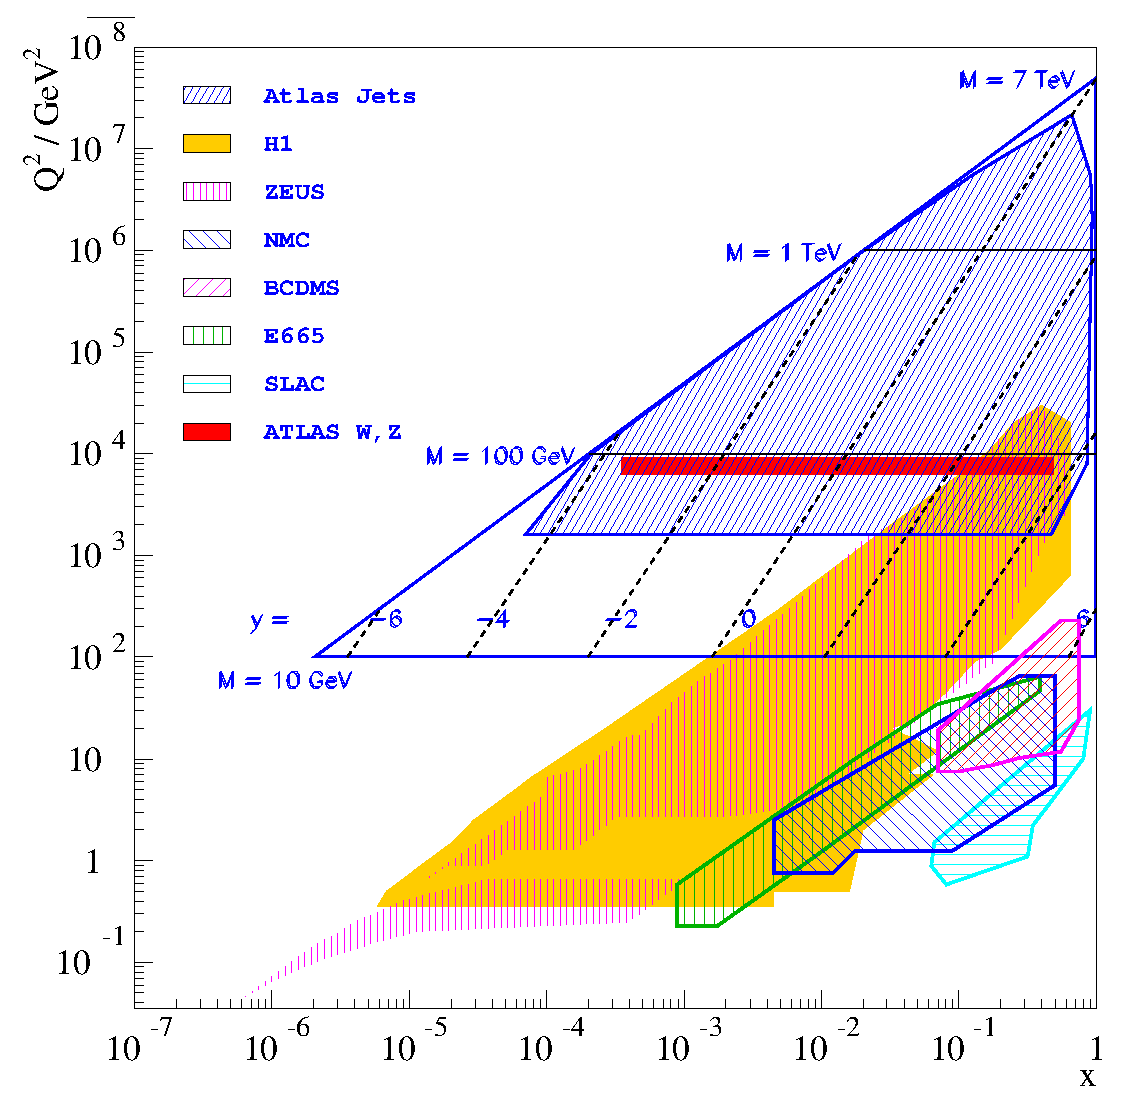
\includegraphics[width=0.65\textwidth]{figures/THEORY_PDF.eps}
\caption{The kinematic plane of various collider experiments in $Q^{2}$ and $x$. In red the range for Z and W production in ATLAS is shown.}
\label{fig:THEORY_PDF}}
\end{figure}

The PDF is a function that shows the probability of finding the given parton in the given hadron with a given momentum. They are constructed based on the experimental data from the $ep$, $pp$, $\antibar{p}$ scattering, and are only applicable for the certain range of $Q^{2}$ and $x$. The coverage of the kinematic plane in $Q^{2}$ and $x$ is shown in Fig.~\ref{fig:THEORY_PDF}. To scale PDFs the evolution equations most be used, such as DGLAP. To accurately predict the results of hadron scattering the set of 13 different PDFs is required, one for each of the 12 quarks ($\bar{t}$,$\bar{b}$,$\bar{c}$,$\bar{s}$,$\bar{u}$,$\bar{d}$,$d$,$u$,$s$,$c$,$b$,$t$) and one for the gluons. The color of the partons can't be determined, so the PDFs are integrated over that degree of freedom. The PDFs for $t$ and $\bar{t}$ are set to zero because of the high mass of the top quark. The PDFs for $b$, $\bar{b}$, $c$ and $\bar{c}$ are only non-zero for $Q^{2} \gg (m_{b})^{2}$.

Sets of PDFs are released by several groups, who mostly utilize the same fitting techniques and are based on the experimental data. Among recent releases can be notet these of the CTEQ-TEA collaboration~\cite{lib:MC_pdfct10}, the MSTW group~\cite{lib:MC_pdfmstw1, lib:MC_pdfmstw2}, the ABM group~\cite{lib:MC_pdfabm}. They provide the sets for LO, NLO, NNLO and also $\alpha_{S}(M_{Z})$ determinations. The HERAPDF group not only released the sets, but also opened their fitting framework for other experiments in order to produce a global fits~\cite{lib:MC_pdfhera}. The NNPDF group used a neural network approach to determine the PDFs with unbiased parameterization~\cite{lib:MC_nnpdf1,lib:MC_nnpdf2,lib:MC_nnpdf3}.

\section{$pp$ collisions and Z boson production}

The proton-proton collisions are the ones that take place in LHC. At low energy, the $pp$ collision looks like elastic scattering of two charged particles. But on the energies on which LHC operates, all collisions are deep inelastic, which means that the internal structure of the proton starts to play a role.

\begin{figure}
\center{
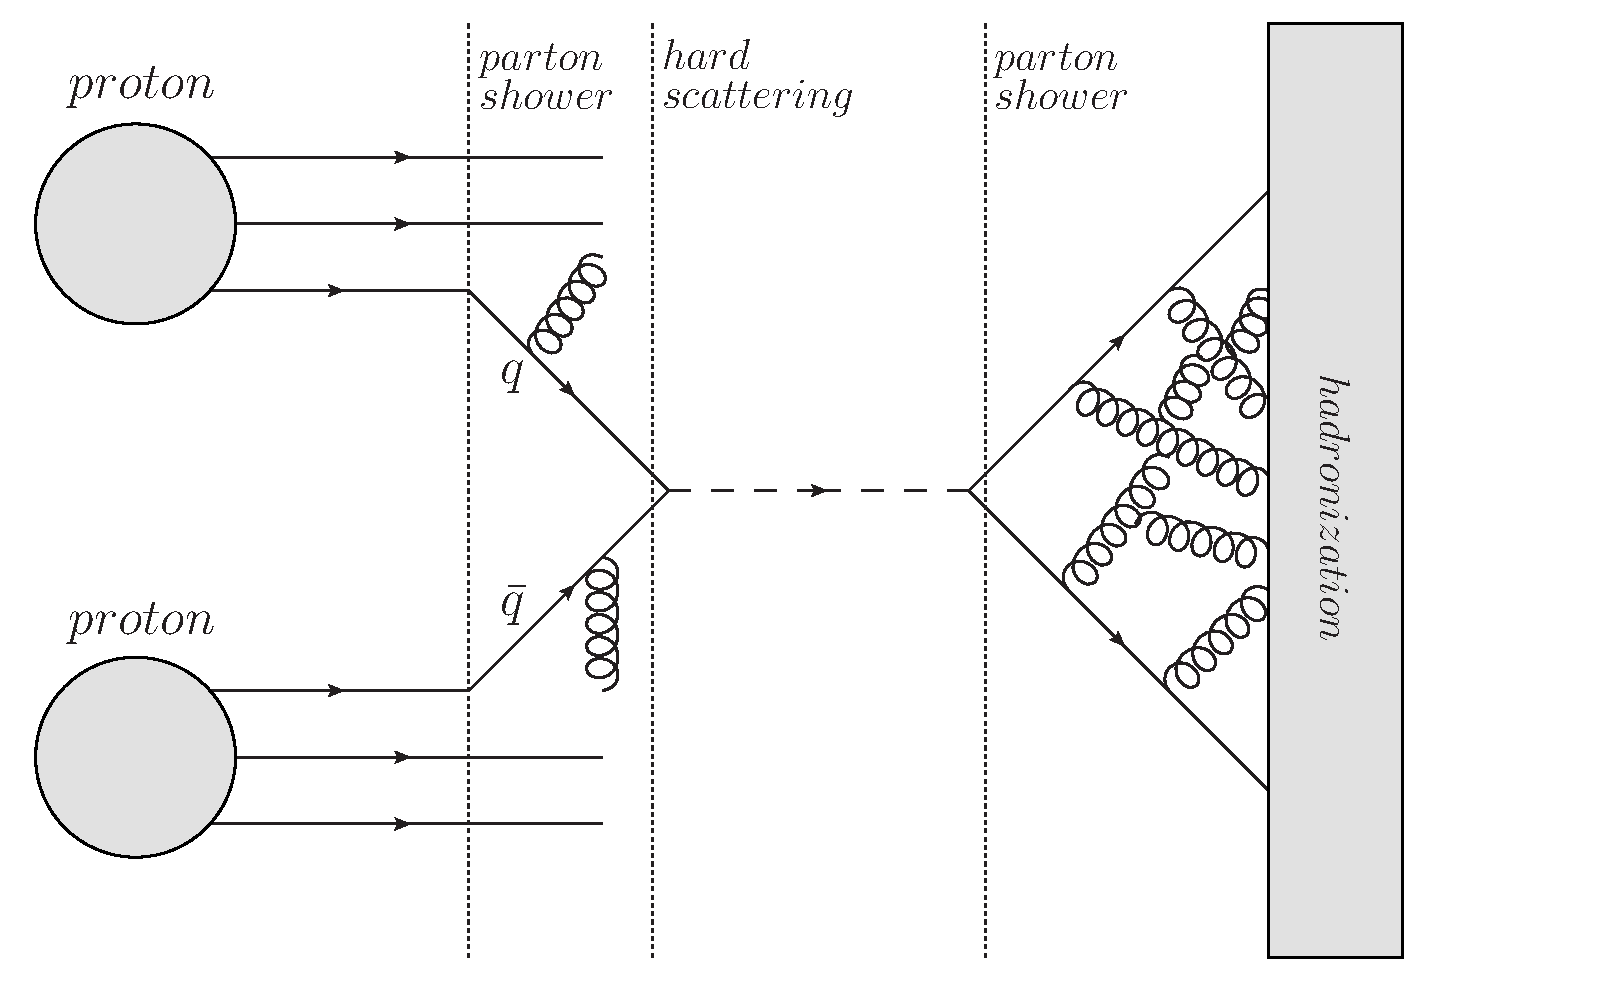
\includegraphics[width=0.8\textwidth]{figures/THEORY_qqbar.eps}
\caption{The deep inelastic scattering of two protons. The three main phases of the process are shown: intial radiation, the hard scattering itself, when the gauge boson is produced, and a final state radiation. If the gauge boson decayed into quarks, the hadronization process takes place in the end, when these quarks decay into color-neutral hadrons.}
\label{fig:THEORY_pp}}
\end{figure}

The process of the $pp$ collision is shown on Fig.~\ref{fig:THEORY_pp}. The three stages of the collision can be calculated by theory, with the use of the perturbative theory, but the difficulty of such calculations for the high orders of radiation processes makes it practically impossible. The three processes are calculated separately, with initial and final state radiations being calculated by the approach called the parton shower: the radiation process of each quark is calculated independently. The hard scattering itself can be calculated in leading order (LO, no radiative corrections), next to leading order (NLO, one radiative corrections), next to next to leading order (NNLO) and so on. Usually one radiative correction is used (NLO), which gives a result with an acceptable error, and is not difficult to calculate.

\begin{figure}
\center{
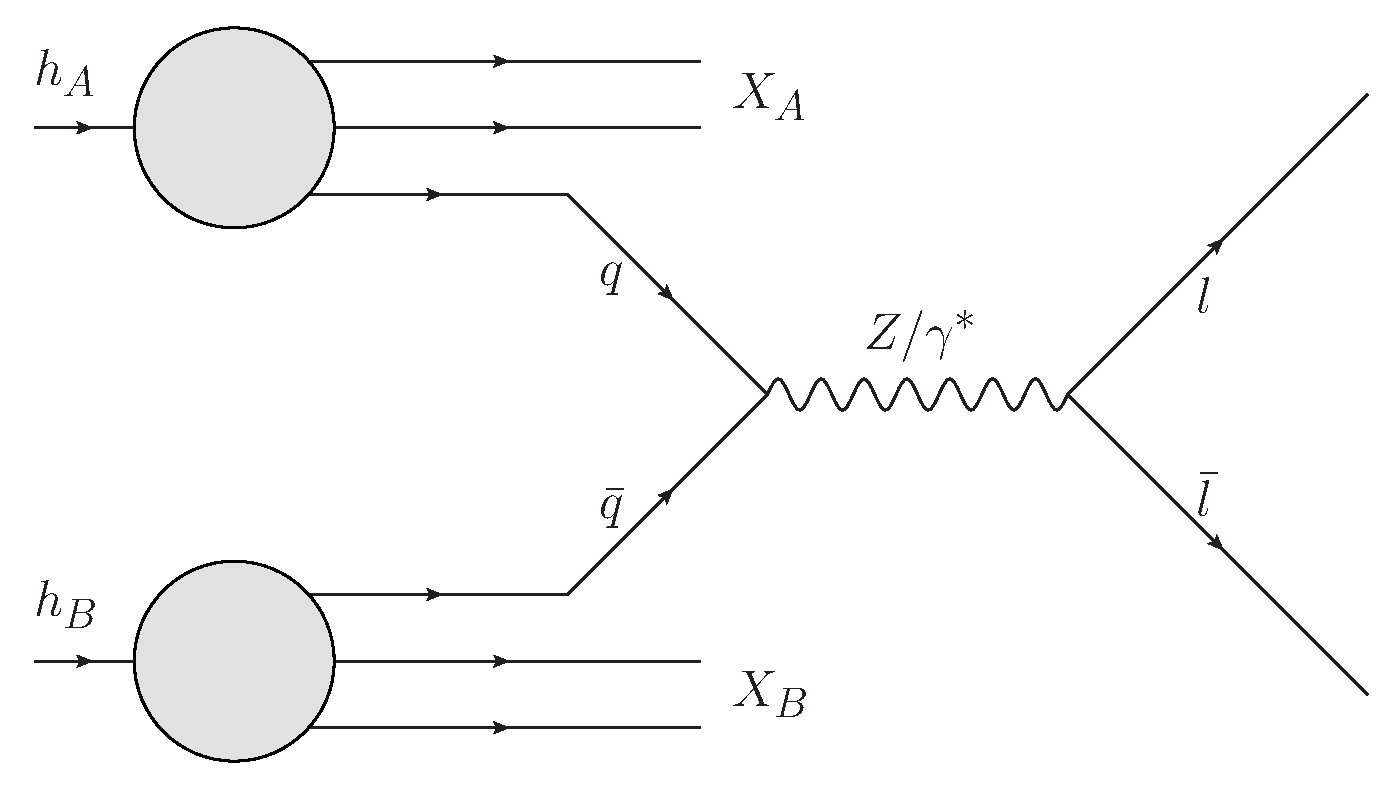
\includegraphics[width=0.8\textwidth]{figures/THEORY_DY.eps}
\caption{The Drell-Yan process in leading order. A quark from one hadron and an antiquark from another annihilate and produce a vector boson (photon or Z) which decays into lepton-antilepton pair. The remaining quarks of the initial hadrons do not interact between each other.}
\label{fig:THEORY_DY}}
\end{figure}

Z boson is produced during the Drell-Yan process, which is shown on Fig.~\ref{fig:THEORY_DY}. The process in leading order (also called the tree-level Drell-Yan) involves only a quark and an antiquark producing a boson which in turn decays into a lepton-antilepton pair.

To properly calculate a theoretical prediction for such a process, the PDFs must be applied to both interacting protons, which complicates the calculations and increases the resulting error. This is common problem of hadron colliders as opposed by lepton or $ep$ ones. But because of it's high rest mass, hadrons can be accelerated to the much higher energies, which makes hadron colliders still preferable for certain tasks despite this shortcoming.

\section{Theoretical predictions for the \Zee\ cross-section}

There are several processes where the events can be clearly filtered from the background. The \Wenu\ and \Zee\ decays are the examples of such processes. The reason for this is because their decays have resonance in LHC, which outstands on the mass-spectrum from the others, like $J/\Psi$, $Y$, and di-boson decays. The electrons and the muons are the particles that undergo reconstruction and identification with best efficiencies, and the aforementioned decays have no hadronization phase which would result in jets, which have poor resolution and scale errors. The cress-section of such processes can thus be measured with high precision, and are important in different aspects.

While the \Zee\ analysis can be used for several things, including the researches on $\alpha_{s}$ constant and forward-backward asymmetry, the main application for the cross-section itself would be the PDF fits. The theoretical prediction for the Drell-Yan \Zgee\ process in LO is as follows~\cite{lib:theory_Z-c-s}:

\begin{equation}
\frac{d^{2}\sigma}{dM_{ee}dy} = \frac{4\pi\alpha^{2}_{s}(M_{ee})}{9}2M_{ee}\cdot P(M_{ee})\cdot\Phi(x_{1},x_{2},M^{2}_{ee})\,.
\end{equation}

Here the $M_{ee}$ is the mass of the boson, the $y$ is the boson rapidity, the $P(M)$ is the propagator term and the $\Phi(x_{1},x_{2},M^{2})$ the parton distribution function that depends on the $x$ parameter of both quark and antiquark. This cross-section is a sum of contribution from both $Z$ and $\gamma^*$ process as well as interference thereof. For the photon process the propagator and the PDF are given as

\begin{equation}
P_{\gamma}(M_{ee}) = \frac{1}{M^{4}_{ee}}\,,\,\;\Phi_{\gamma} = \sum_{q} e^{2}_{q} F_{\qqbar} \,.
\end{equation}

It can be seen that the propagator term $P_{\gamma}$ suppresses the photon contribution for the high-mass ($M_{ee} \gg M_{Z}$) and the mass peak ($M_{ee} \approx M_{Z}$) analyses.

For the $Z/\gamma$ interference contribution the same terms can be given as

\begin{equation}
\begin{gathered}
P_{Z\gamma}(M_{ee}) = \frac{k_{Z} \cdot v_{e} \cdot (M_{ee}^{2} - M_{Z}^{2})}{M_{ee}^{2} \cdot ((M_{ee}^{2} - M_{Z}^{2})^{2} + (\Gamma_{Z}M_{Z})^{2})}\,,\,\;
\Phi_{Z\gamma} = \sum_{q} 2e_{q}v_{q} F_{\qqbar} \,,\\
k_{Z} = \frac{1}{4\sin^{2}\theta\cos^{2}\theta} \,, \,\; \cos\theta = \frac{M_{W}}{M_{Z}} \,,
\end{gathered}
\end{equation}

Where $\theta$ is a $\theta_{W}$ - a weak mixing angle. The contribution of this component is proportional to the vector coupling of the electron $v_{e}$, which is close to zero, so the contribution is also negligible.

And finally for the \Zee\ process itself the terms are as follows:

\begin{equation}
P_{Z}(M_{ee}) = \frac{k^{2}_{Z} \cdot (v^{2}_{e} + a^{2}_{e})}{(M^{2}_{ee} - M^{2}_{Z})^{2} + (\Gamma_{Z}M_{Z})^{2}}\,,\,\;
\Phi_{Z} = \sum_{q} (v^{2}_{q} + a^{2}_{q}) F_{\qqbar} \,.
\end{equation}

As it is seen from this, the PDFs are included in the cross-section formula as a direct factor, so the double-differential cross section can be directly used to conduct the PDF fits.

It is important to note, that only $\sim$3\% of the produced $Z$ bosons decay into electrons. About 70\% decay into gluons, which results in jets, and suffer from bad analysis efficiency. About 20\% go into neutrinos, and are not detected at all, and only $\sim$10\% are lepton decays, which are divided roughly equally between electrons, muons and taus. So both \Zee\ and \Zmm\ analyses are equally important, while \Ztau\ is impossible to conduct due to very short life of $\tau$ particles. We consider \Ztau\ events a background.

The electrons and muons are detected by the different parts of the ATLAS, and thus these particles are detected in different parts of the kinematic space (see Sec.~\ref{sec:ATLAS} for more details). The EM calorimeters that detect electrons have a coverage of $|\eta| < 5.2$, while muon chambers have $|\eta| < 2.4$. These differences in the kinematic coverage poses a problem when we want to cobine the results of the different analyses for the better statistics. In order to overcome this problem the cross-sections are calculated in (i.e. extrapolated to) the common fiducial volume (more on that in Sec.~\ref{sec:ZeeCrossSec}).

\chapter{The LHC (Large Hadron Collider)}
\label{sec:LHC}

The LHC is the largest circular collider in the world, which is designed to deliver $pp$ collisions with energies up to 14 TeV and instantaneous luminosity up to $10^{34} cm^{-2}s^{-1}$. The instantaneous luminosity is the parameter, representing the proportionality of the event rate and the cross-section for a given process: $N = \mathcal{L} \cdot \sigma$. The parameters is thus process-agnostic, and describes the collider itself in a way that it helps to estimate the amount of collisions happening in the detector. The derivative from this parameter is a pileup, which is the amount of collisions per detector readout. With the increasing of the luminosity, the pileup also increases, flooding the detector with the particles from different processes, making it hard to reconstruct the event. The techniques to overcome the pileup problem will be discussed in Sec.~\ref{sec:Reconstruction}.

The LHC complex includes several accelerators with different sizes of rings which gradually increase the energy of the particles. All of them are shown on the Fig.~\ref{fig:LHC}.

\begin{figure}
\center{
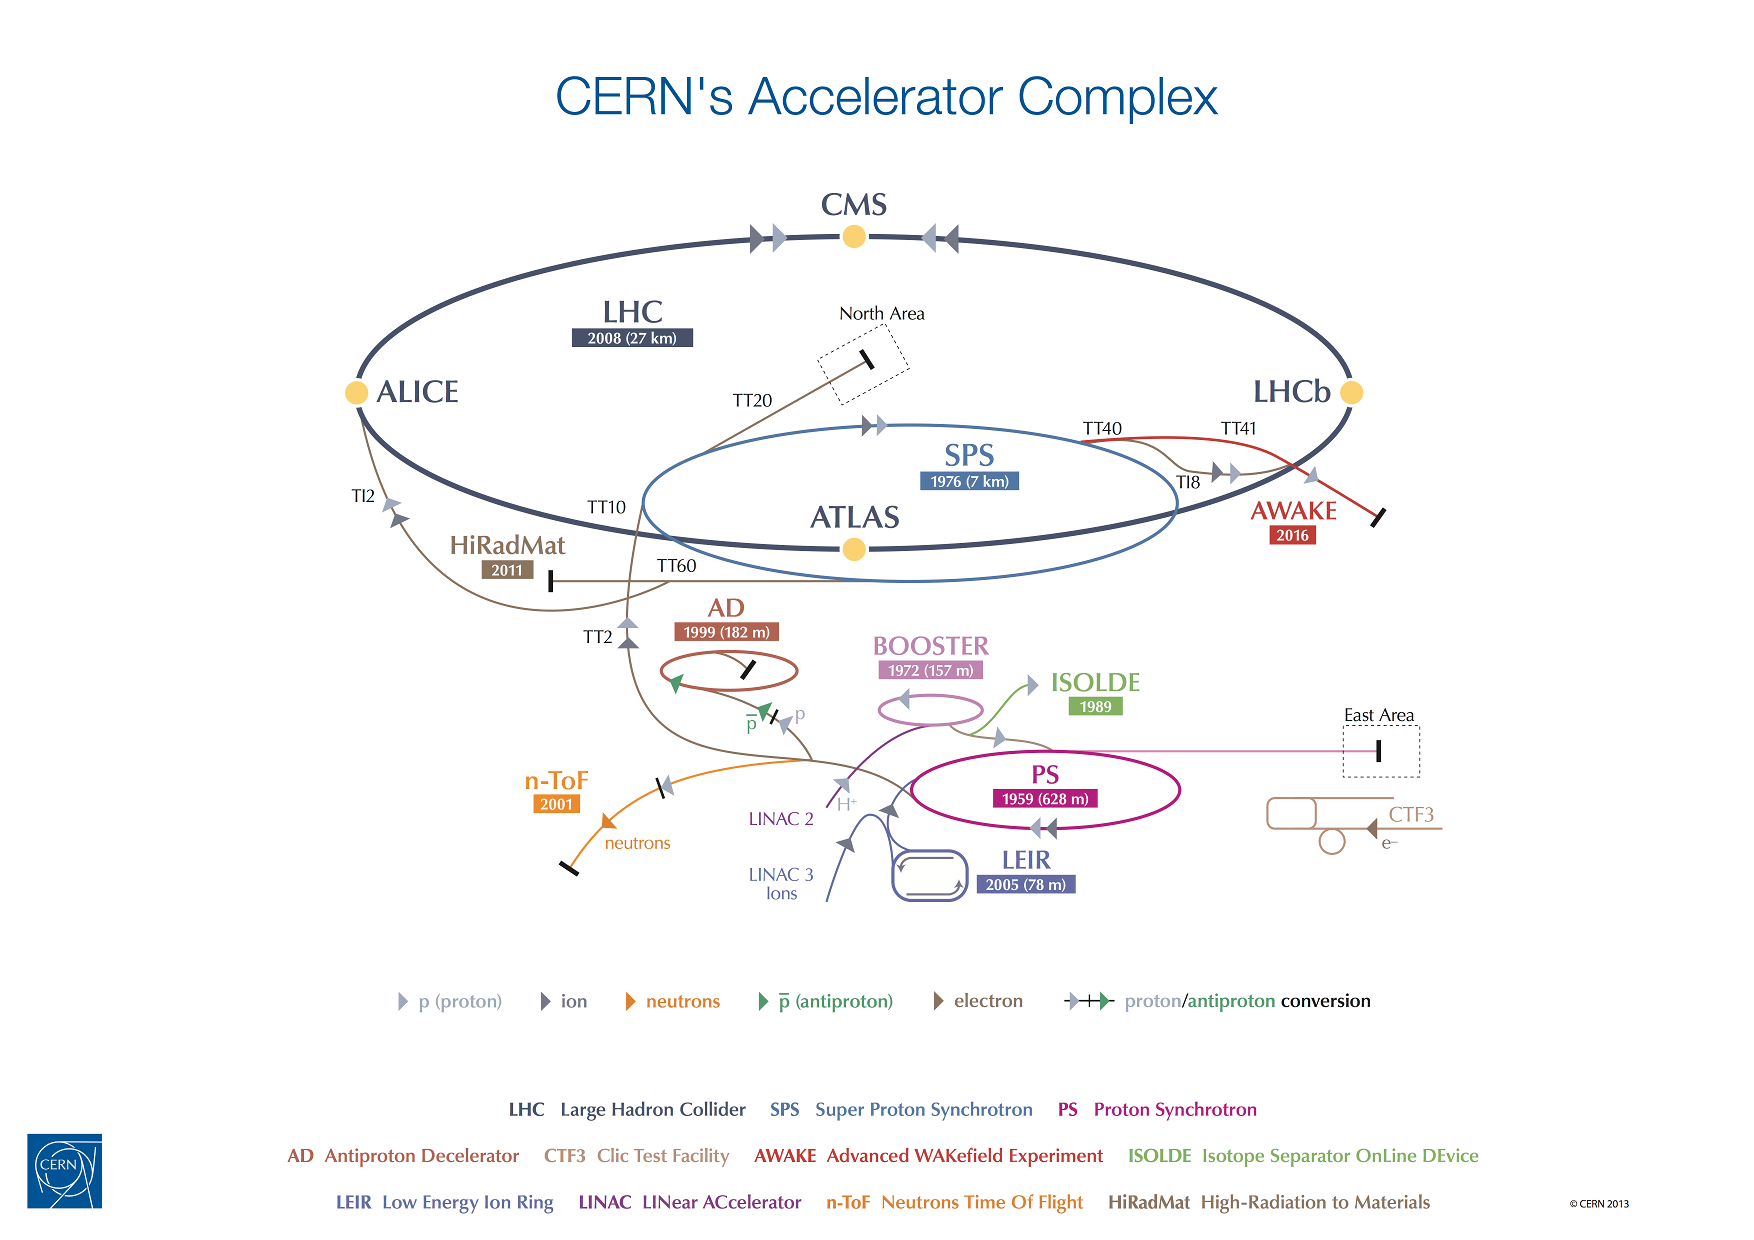
\includegraphics[width=1.0\textwidth]{figures/LHC.png}
\caption{The LHC accelerator complex. For each accelerator the year of completion is shown. For circular accelerators the length of the ring is also shown.}
\label{fig:LHC}}
\end{figure}

The full acceleration process of the protons looks like this:

\begin{enumerate}
\item The protons are injected into the Linear Accelerator 2 (Linac2). In case of lead ions Linac3 is used.
\item In case of protons, the bunches are then accelerated in the Proton Synchrotron Booster (Booster), while for heavy ions the Low Energy Ion Ring (LEIR) is used. Both of them pass the accelerated particles to Proton Synchrotron (PS) for storage until the needed amount of particles is pre-accelerated.
\item Next is the Proton Synchrotron - the first high-energy accelerator in this chain, its outputs is 25 GeV, and it was the largest CERN accelerator up until 1970s.
\item The next is the last preparatory accelerator in chain: the Super Proton Synchrotron (SPS). It also once was the most prominent CERN collider and, among other things, lead to the discovery of W and Z bosons during the experiments with \antibar{p} collisions. Its output energy is 450 GeV.
\end{enumerate}

After LHC is filled with the pre-accelerated particles, it starts its own acceleration process. It takes about 20 minutes to reach the energy of 3.5 TeV on which the collision took place during 2011. Next is preparatory stage during which the bunches are focused in order to increase luminosity. If all goes well, the LHC goes into the state of "stable beams": the collisions are started and the detectors can start recording the data. Eventually, the beams loose their focus, the data-taking then stops, and the beams are dumped. The data-taking period is usually several hours long (up to 20) and ideally it lasts as long as the beams circulate the ring, but sometimes other problems arise which prevent data-taking for a period of time during the circulation.

There are 6 detectors which record data from the collisions on LHC.
\begin{itemize}
\item {\bfseries ALICE (A Large Ion Collider Experiment)} This detector is designed to analyze heavy-ion collisions.
\item {\bfseries ATLAS (A Toroidal LHC ApparatuS) and CMS (Compact Muon Solenoid)} These are two general-purpose detectors which cover a wide range of HEP fields. They have differences in design though: ATLAS has less matter in the calorimeter and better muon detectors, while CMS is twice as heavy as ATLAS (has twice as much matter) and because of this has better EM calorimeter, but the detection of hadrons and muons is less precise.
\item {\bfseries LHCb (LHC-beauty)} This detector studies the b-quarks.
\item {\bfseries LHCf (LHC-forward)} This detector studies the forward particles, which behave similar to cosmic rays.
\item {\bfseries TOTEM (TOTal Electric and diffractive cross-section Measurement)} This detector measures the total $pp$ cross-section.
\end{itemize}

Each detector operates independently from one another to enable cross-checking between experiments and increase the trustworthiness of the results.

During 2011 the LHC operated with the same energy of 3.5 TeV per beam and with more or less same luminosity: the difference between the beginning of the data taking in april and the end in december is only about 4 times, as opposed to the ten thousand times, in which the luminosity increased during 2010 data taking. More on the data samples can be seen in Chapter~\ref{sec:DataSamples}.

\chapter{The ATLAS Experiment}
\label{sec:ATLAS}

The ATLAS detector is one of the two general purpose detectors on LHC, and is designed for probing for p-p and A-A collisions.
This detector represents the work of a large collaboration of several thousand physicists, engineers and technicians over a period of fifteen years of dedicated design, development, fabrication, and installation. There are several fields in which the resarches are currently going in ATLAS collaboration, including Z and W boson decay, search for Higgs boson,
supersymmetry, study on B-mesons, and others. This broad spectrum of researches makes high demands on the detector's complexity and the precision
of the different sub-systems.

\section{Physics requirements and detector overview}
\label{sec:ATLAS_overview}
The ATLAS detector has a cylindric shape, it is aligned along the beam line with the center situated at the interaction point.
The coordinate system that is used to describe the detector follows its natural geometry. the interaction point is taken as an origin,
while the $z$ axis is put along the beam pipe, making the $x$-$y$ plane transverse. The positive $x$-axis is defined to be pointing to the center
of the LHC ring, and positive $y$-axis is defined to be pointing upwards. The direction on the $z$-axis is picked such as to form a right-handed coordinate system.
The azimuthal angle $\varphi$ is measured as usual around the beam axis, and the polar angle $\theta$ is the angle from the beam axis. The rapidity $y$ and pseudorapidity $\eta$
are calculated using the standard definition:

\begin{align}
y &= \frac{1}{2} \log \left(\frac{E+p_z}{E-p_z}\right)\,, \\
\eta &= - \log (\tan (\frac{\theta}{2}))\,.
\end{align}

\begin{figure}
\center{
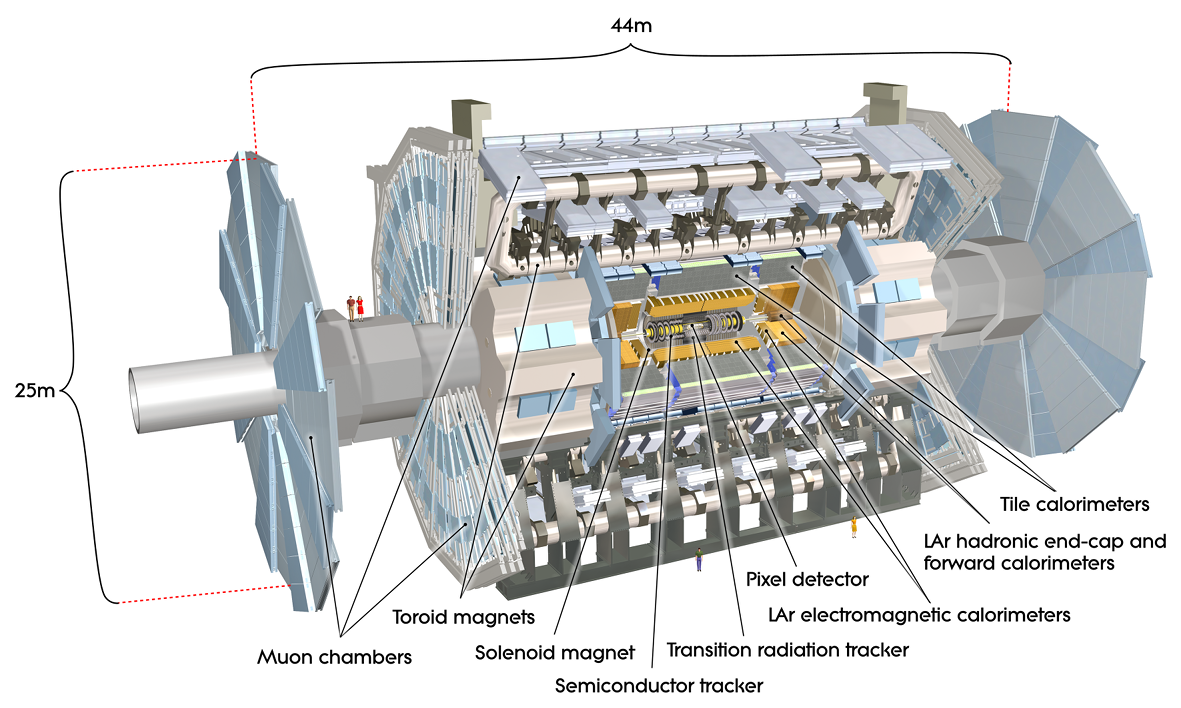
\includegraphics[width=1.0\textwidth]{figures/ATLAS_overview.eps}
\caption{Overview of the ATLAS detector, with all the major sub-systems and the human-sized scale figures~\cite{lib:ATLASdet}.}
\label{fig:ATLAS_overview}}
\end{figure}

The overview of the ATLAS detector is shown on the Fig.~\ref{fig:ATLAS_overview}. The main detector sub-systems can be seen there: the innermost is the tracker, then goes the EM calorimeters, then the hadronic calorimeters, and finally the muon spectrometers. There is also a magnet system, which is not a detector by itself, but is essential to the functioning of the whole system. All of the sub-detectors are briefly described below.

\begin{itemize}
\item The tracker (also called "the inner detector") records the tracks of the particles and is used to determine the charge and momentum.
\item The EM calorimeters identify and measure the energy of EM particles: electrons, positrons and photons.
\item The hadronic calorimeters measure the energy of hadrons.
\item The muon spectrometers identify and measure the energy, momentum and charge of the muons.
\end{itemize}

Based on their physical properties, different particles behave differently in these sub-detectors. The reconstruction of the particles rely heavily on the traces that particles leave or do not leave in different parts of the detector.

\begin{itemize}
\item {\bfseries Photons}, unless converted to the electrons, do not leave tracks in the tracker. Stop in the EM calorimeter and leave a cluster of the deposited energy in it.
\item {\bfseries Electrons} leave a track in the tracker, in the EM calorimeter behave similarly to photons: leave cluster with similar shape and properties.
\item {\bfseries Charged mesons and protons} leave a track in the tracker, leave a cluster deep in the EM calorimeter, which can be distinguished from the EM particles, stop in the hadronic calorimeter, leaving a cluster in it.
\item {\bfseries Neutral mesons and neutrons} do not leave a track, leave a cluster deep in the EM calorimeter, do not propagate to the hadronic calorimeter.
\item {\bfseries Muons} leave a track, leave a recognizable cluster in the calorimeters, which is associated with the so-called "minimum ionizing particles" (MIP), propagate further to the muon chambers and usually are not stopped by the detector.
\item {\bfseries Neutrinos} do not interact with the detector, and leave it without any traces. Are identified by the missing $E_{t}$.
\end{itemize}

\section{Tracking}
\label{sec:ATLAS_tracker}

Because of the very high number of the events per second, the density of the tracks inside the inner detector is also very high. We are getting approximately 1000 particles
from the collision point every 25 ns within the central eta region which we need to record. To achieve the needed momentum and vertex resolution, high-precision measurements must be made with fine detector granularity. The tracker of the ATLAS detector consists of pixel and silicon microstrip (SCT) trackers, and the Transition Radiation Tracker (TRT). Combined they provide these features.

\begin{figure}
\center{
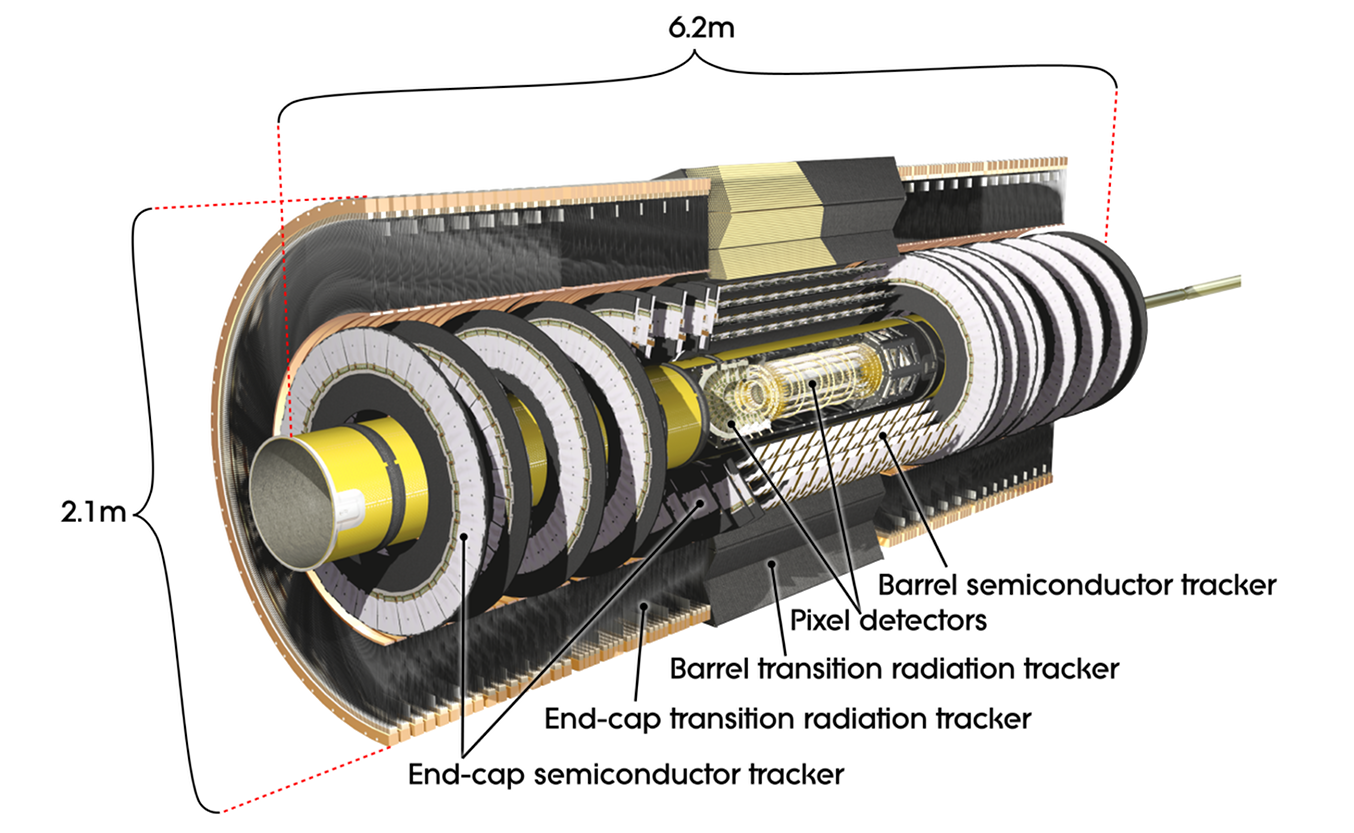
\includegraphics[width=1.0\textwidth]{figures/ATLAS_tracker.eps}
\caption{Overview of the ATLAS tracker. The SCT, TRT and pixel detectors are shown there~\cite{lib:ATLASdet}.}
\label{fig:ATLAS_tracker}}
\end{figure}

The layout of the tracker is illustrated in Fig.~\ref{fig:ATLAS_tracker}. Its
basic parameters are summarised in Tab.~\ref{tab:ATLAS_tracker}. The magnetic field with the intencity of $2T$ generated by the central solenoid covers most of the tracker: it extends over a length of $5.3 m$ with a diameter of $2.5 m$. The precision tracking detectors (pixels and SCT) cover the region
$|\eta|<2.5$. As can be seen on the picture, in the central area they are arrengad in concentric cylinders along the beam axis, while in the end-cap regions they are arranged in form of discs perpendicular to the beam. The highest granularity is achieved around the interaction point using silicon pixel detectors. The pixel layers are
segmented in $\varphi$ and $z$ with typically three pixel layers crossed by each track. All pixel sensors
are identical and have a minimum pixel size in $R-\varphi \times z-\varphi$ of $50 \times 400 \mu m^2$. The intrinsic accuracies
in the central region are $10 \mu m$ $(\varphi)$ and $115$ $\mu m$ $(z)$ and in the end-cap regions are $10 \mu m$ $(\varphi)$ and $115 \mu m$ $(R)$.
The pixel detector has approximately 80.4 million readout channels. For the SCT, eight strip layers
(four space points) are crossed by each track. In the central region, this detector uses small-angle
($40 mrad$) stereo strips to measure both coordinates, with one set of strips in each layer parallel to
the beam direction, measuring $R-\varphi$. They consist of two $6.4 cm$ long daisy-chained sensors with
a strip pitch of $80 \mu m$. In the end-cap region, the detectors have a set of strips running radially and
a set of stereo strips at an angle of $40 mrad$. The mean pitch of the strips is also approximately
$80 \mu m$. The intrinsic accuracies per module in the barrel are $17 \mu m$ $(\varphi)$ and $580 \mu m$ $(z)$ and in
the disks are $17 \mu m$ $(\varphi)$ and $580 \mu m$ $(R)$. The total number of readout channels in the SCT is
approximately 6.3 million.

\begin{table}
\centering
\begin{tabular}{ll | r@{$<$}c@{$<$}l | r@{$<$}c@{$<$}l} \hline\hline
\multicolumn{2}{l|}{\bf Item} & \multicolumn{3}{c|}{\bf Radial extension (mm)} & \multicolumn{3}{c}{\bf Length (mm)} \\\hline
\multicolumn{2}{l|}{\bf Overall tracker envelope} & $0$&$R$&$1150$ & $0$&$|z|$&$3512$ \\
\multicolumn{2}{l|}{\bf Beam-pipe} & $29$&$R$&$36$ & \multicolumn{3}{c}{}\\\hline
{\bf Pixel} & Overall envelope & $45.5$&$R$&$242$ & $0$&$|z|$&$3092$ \\
3 cylindrical layers & Sensitive barrel & $50.5$&$R$&$122.5$ & $0$&$|z|$&$400.5$ \\
$2*3$ disks & Sensitive end-cap & $88.8$&$R$&$149.6$ & $495$&$|z|$&$650$ \\
\multicolumn{2}{l|}{} & \multicolumn{3}{c|}{} & \multicolumn{3}{c}{}\\
{\bf SCT} & Barrel envelope & $255$&$R$&$549$ & $0$&$|z|$&$805$ \\
 & End-cap envelope & $251$&$R$&$610$ & $810$&$|z|$&$2797$ \\
4 cylindrical layers & Sensitive barrel & $299$&$R$&$514$ & $0$&$|z|$&$749$ \\
$2*9$ disks & Sensitive end-cap & $275$&$R$&$560$ & $839$&$|z|$&$2735$ \\
\multicolumn{2}{l|}{} & \multicolumn{3}{c|}{} & \multicolumn{3}{c}{}\\
{\bf TRT} & Barrel envelope & $554$&$R$&$1082$ & $0$&$|z|$&$780$ \\
 & End-cap envelope & $617$&$R$&$1106$ & $827$&$|z|$&$2744$ \\
73 straw panels & Sensitive barrel & $563$&$R$&$1066$ & $0$&$|z|$&$712$ \\
160 straw panels & Sensitive end-cap & $644$&$R$&$1004$ & $848$&$|z|$&$2710$ \\
\hline\hline
\end{tabular}
\caption{The description of the geomentry of the ATLAS tracker~\cite{lib:ATLASdet}.}
\label{tab:ATLAS_tracker}
\end{table}

A large number of hits (typically 36 per track) is provided by the 4 mm diameter straw tubes
of the TRT, which enables track-following up to $|\eta|=2.0$. The TRT only provides $R-\varphi$ information, for which it has an intrinsic accuracy of $130 \mu m$ per straw. In the central region, the straws are
parallel to the beam axis and are $144 cm$ long, with their wires divided into two halves, approximately at $\eta = 0$. In the end-cap region, the $37 cm$ long straws are arranged radially in wheels. The
total number of TRT readout channels is approximately 351 thousands.

The combination of precision trackers close to interaction point with the TRT at a larger radius gives very
robust pattern recognition and high precision in all $R$ $\varphi$ and $z$ coordinates. The straw hits at the
outer radius contribute significantly to the momentum measurement, since the lower precision per
point compared to the silicon is compensated by the large number of measurements and longer
measured track length.
The inner detector system provides tracking measurements in a range matched by the precision measurements of the electromagnetic calorimeter. The electron identification capabilities
are enhanced by the detection of transition-radiation photons in the xenon-based gas mixture of
the straw tubes. The semiconductor trackers also allow impact parameter measurements and vertexing for heavy-flavour and $\tau$-lepton tagging. The secondary vertex measurement performance is enhanced by the innermost layer of pixels, at a radius of about $5 cm$.


\section{EM calorimeters}
\label{sec:ATLAS_EM_calo}

\begin{figure}
\center{
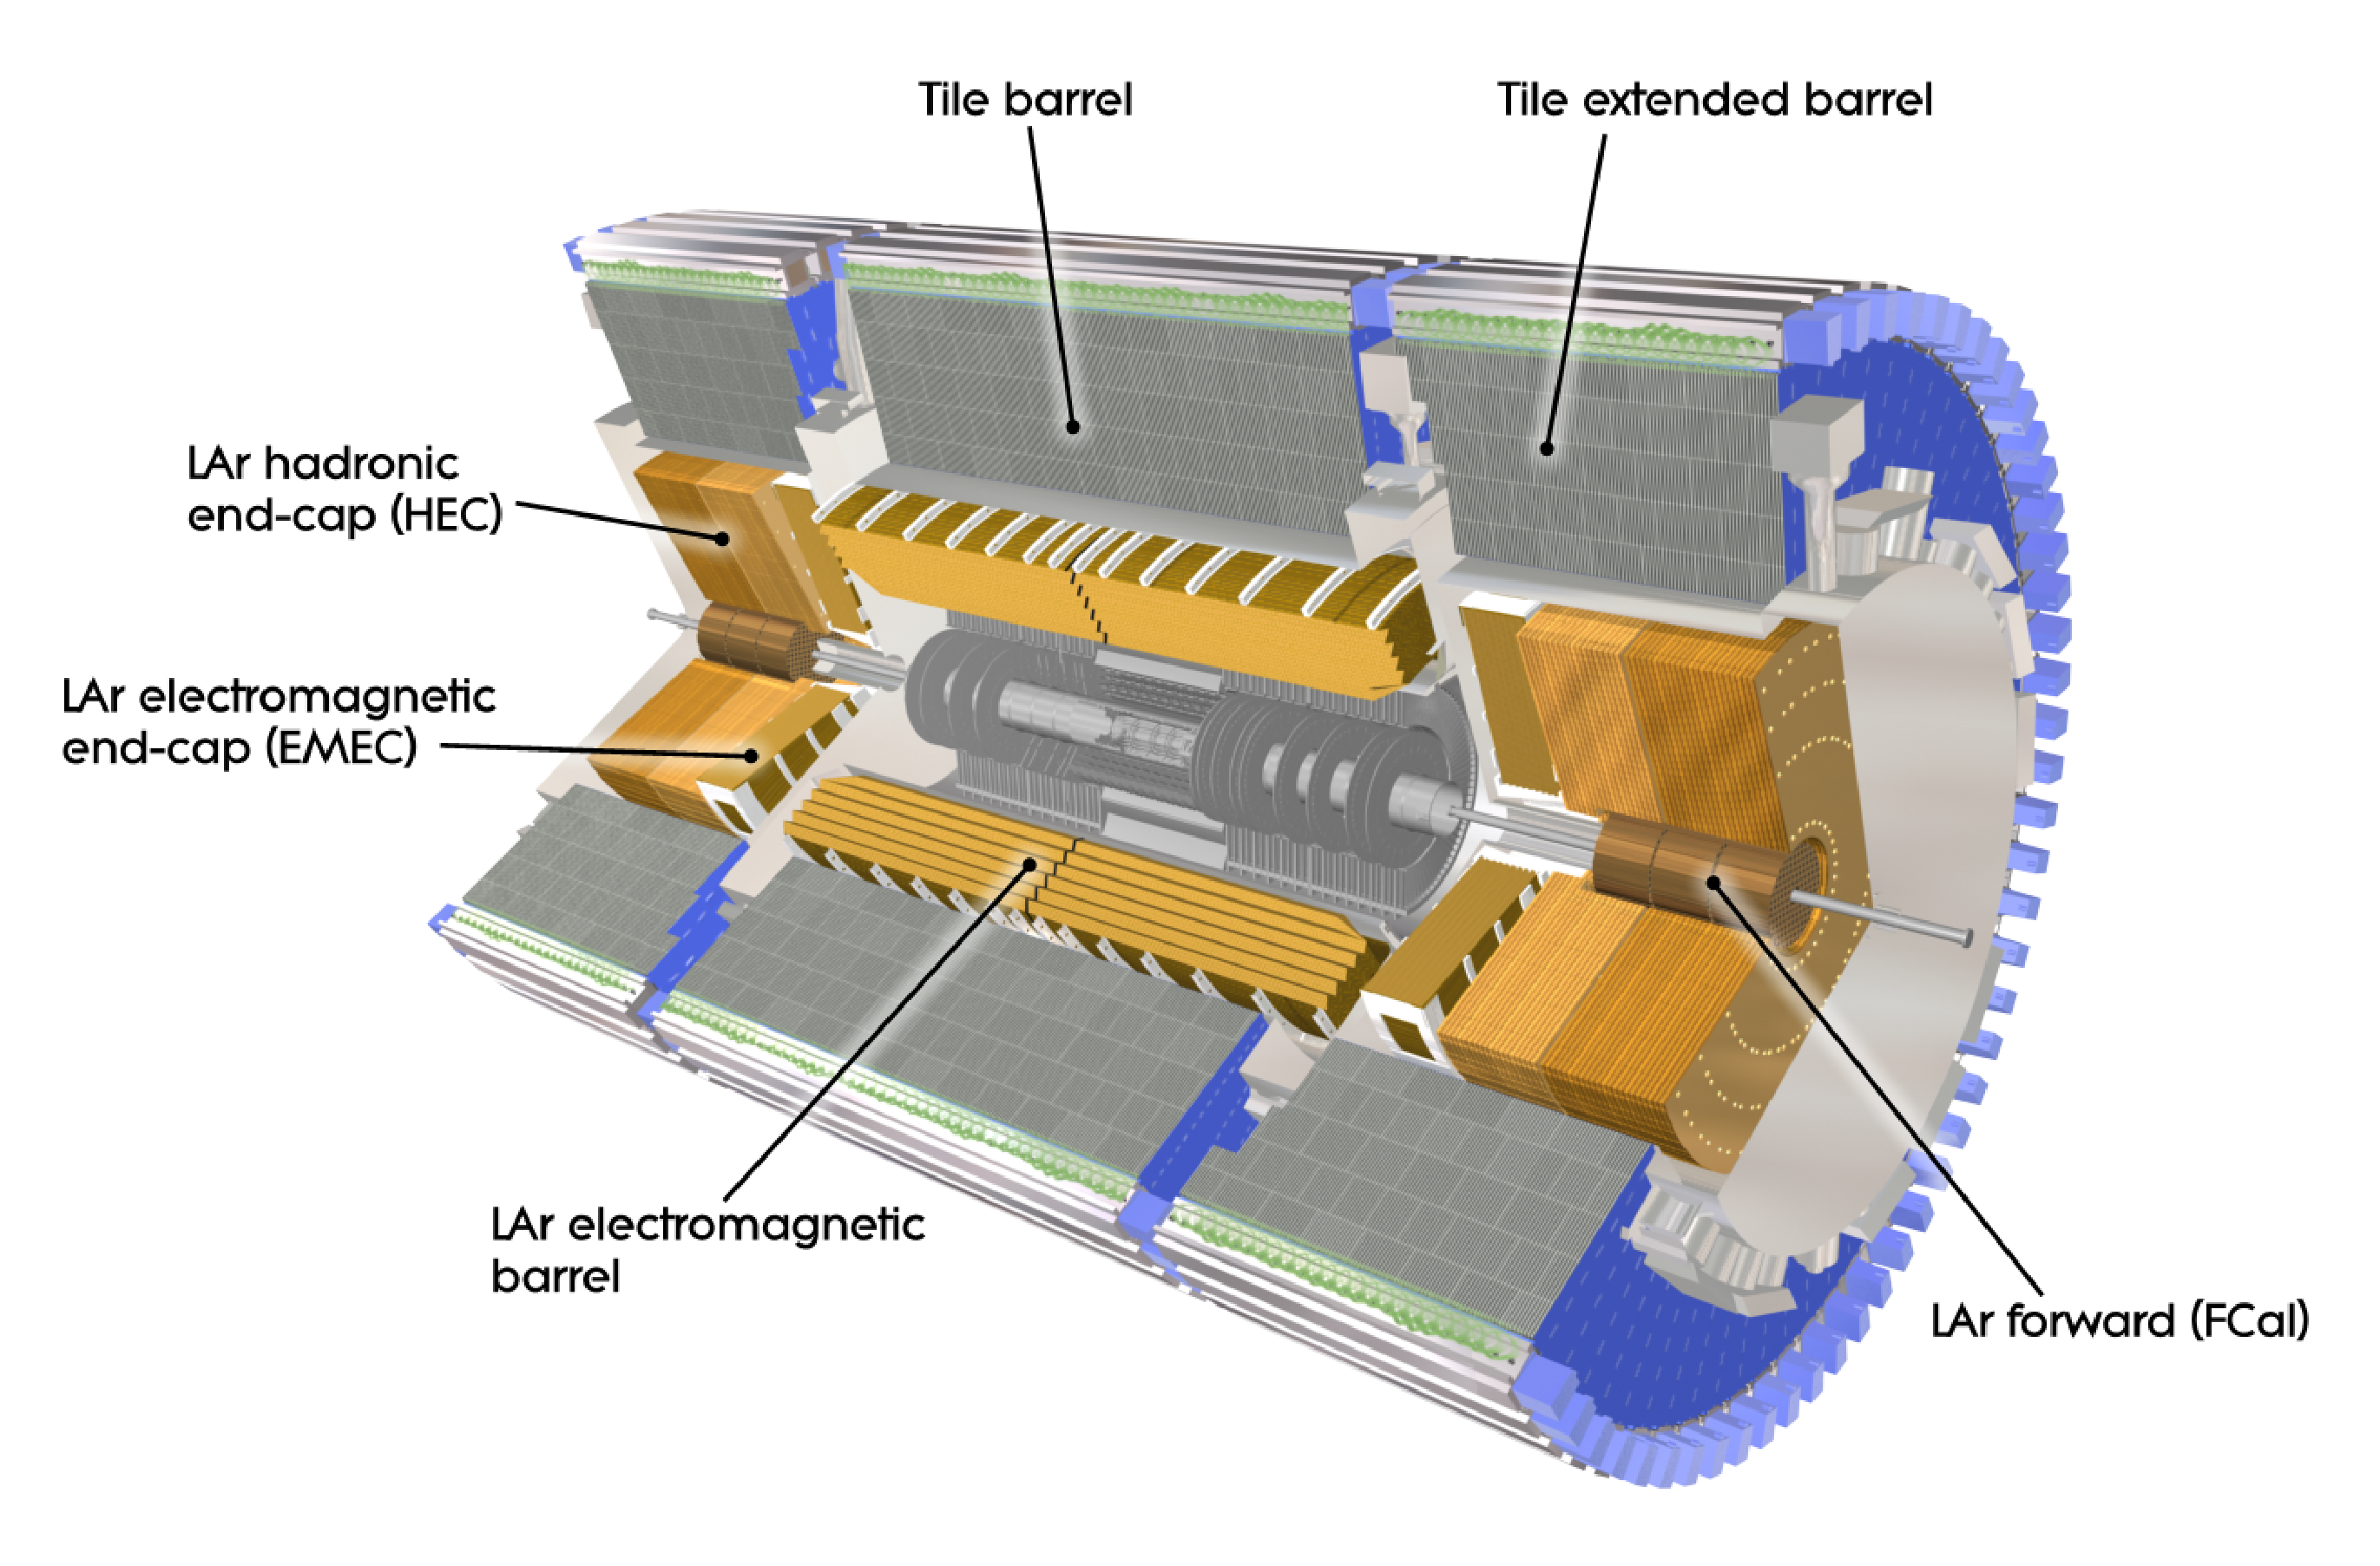
\includegraphics[width=1.0\textwidth]{figures/ATLAS_calo.eps}
\caption{Overview of the ATLAS EM and hadronic calorimeters.~\cite{lib:ATLASdet}.}
\label{fig:ATLAS_calorimeter}}
\end{figure}


The EM calorimeter is divided into a barrel (central) part ($|\eta| < 1.475$) and two end-cap components
($1.375 < |\eta| < 3.2$), each housed in their own cryostat. The position of the central solenoid in
front of the EM calorimeter demands optimisation of the material in order to achieve the desired calorimeter
performance. As a consequence, the central solenoid and the LAr calorimeter
share a common vacuum vessel, thereby eliminating two vacuum walls. The barrel calorimeter
consists of two identical half-barrels at positive and negative etas, separated by a small gap (4 mm) at z = 0. Each end-cap
calorimeter is mechanically divided into two coaxial wheels: an outer wheel covering the region
$1.375 < |\eta| < 2.5$, and an inner wheel covering the region $2.5 < |\eta| < 3.2$. The EM calorimeter is
a lead-LAr detector with accordion-shaped kapton electrodes and lead absorber plates over its full
coverage. The accordion geometry provides complete $\varphi$ symmetry without azimuthal cracks. The lead thickness in the absorber plates has been optimised as a function of $\eta$ in terms of EM calorimeter performance in energy resolution. Over the region devoted to central analysis ($|\eta| < 2.5$), the
EM calorimeter is segmented in three sections in depth. For the end-cap inner wheel, the calorimeter is segmented in two sections in depth and has a coarser lateral granularity than for the rest of the acceptance.

In the region of $|\eta| < 1.8$, a presampler detector is used to correct for the energy lost by
electrons and photons upstream of the calorimeter. The presampler consists of an active LAr layer
of thickness 1.1 cm in the barrel and 0.5 cm in the end-cap regions.


\section{Hadronic calorimeters}
\label{sec:ATLAS_H_calo}


The hadronic calorimeter consists of the tile calorimeter (the central part) and the hadronic end-cap calorimeter (HEC).

The tile calorimeter is placed directly outside the EM calorimeter envelope. Its
cantral barrel covers the region $|\eta| < 1.0$, and its two extended barrels cover the range $0.8 < |\eta| < 1.7$. It is a
sampling calorimeter using steel as an absorber and scintillating tiles as active material. Both
barrel and extended barrels are divided azimuthally into 64 modules. Radially, the tile calorimeter
extends from an inner radius of 2.28 m to an outer radius of 4.25 m. It is segmented in depth in three
layers, approximately 1.5, 4.1 and 1.8 interaction lengths ($\lambda$) thick for the barrel and 1.5, 2.6, and
3.3 $\lambda$ for the extended barrel. The total detector thickness at the outer edge of the tile-instrumented
region is 9.7 $\lambda$ at $\eta=0$. Two sides of the scintillating tiles are read out by wavelength shifting
fibres into two separate photomultiplier tubes. In $\eta$, the readout cells built by grouping fibres into
the photomultipliers are pseudo-projective towards the interaction region.

The Hadronic End-cap Calorimeter (HEC) consists of two
independent wheels per end-cap, located directly behind the end-cap electromagnetic calorimeter
and sharing the same LAr cryostats. To reduce the drop in material density at the transition between
the end-cap and the forward calorimeter (around $|\eta| = 3.1$), the HEC extends out to $|\eta| = 3.2$,
thereby overlapping with the forward calorimeter. Similarly, the HEC $\eta$ range also slightly overlaps
that of the tile calorimeter ($|\eta| < 1.7)$ by extending to $|\eta| = 1.5$. Each wheel is built from 32
identical wedge-shaped modules, assembled with fixtures at the periphery and at the central bore.
Each wheel is divided into two segments in depth, for a total of four layers per end-cap. The wheels
closest to the interaction point are built from 25 mm parallel copper plates, while those further away
use 50 mm copper plates (for all wheels the first plate is half-thickness). The outer radius of the
copper plates is 2.03 m, while the inner radius is 0.475 m (except in the overlap region with the
forward calorimeter where this radius becomes 0.372 m). The copper plates are interleaved with
8.5 mm LAr gaps, providing the active medium for this sampling calorimeter.

\section{Forward calorimeters}
\label{sec:ATLAS_FCAL}

The forward calorimeter (FCAL) covers the biggest eta range ($3.1 < |\eta| < 4.9$) and combines both EM and hadronic parts.

It is integrated into the end-cap cryostats, as this provides
clear benefits in terms of uniformity of the calorimetric coverage as well as
reduced radiation background levels in the muon spectrometer. In order to reduce the amount of
neutron albedo in the inner detector cavity, the front face of the FCAL is recessed by about 1.2 m
with respect to the EM calorimeter front face. This severely limits the depth of the calorimeter
and therefore calls for a high-density design. The FCAL is approximately 10 interaction lengths
deep, and consists of three modules in each end-cap: the first, made of copper, is optimised for
electromagnetic measurements, while the other two, made of tungsten, measure predominantly the
energy of hadronic interactions. Each module consists of a metal matrix, with regularly spaced
longitudinal channels filled with the electrode structure consisting of concentric rods and tubes
parallel to the beam axis. The LAr in the gap between the rod and the tube is the sensitive medium.
This geometry allows for excellent control of the gaps, which are as small as 0.25 mm in the first
section, in order to avoid problems due to ion buildup.

\section{Muon spectrometers}
\label{sec:ATLAS_muon_chambers}

\begin{figure}
\center{
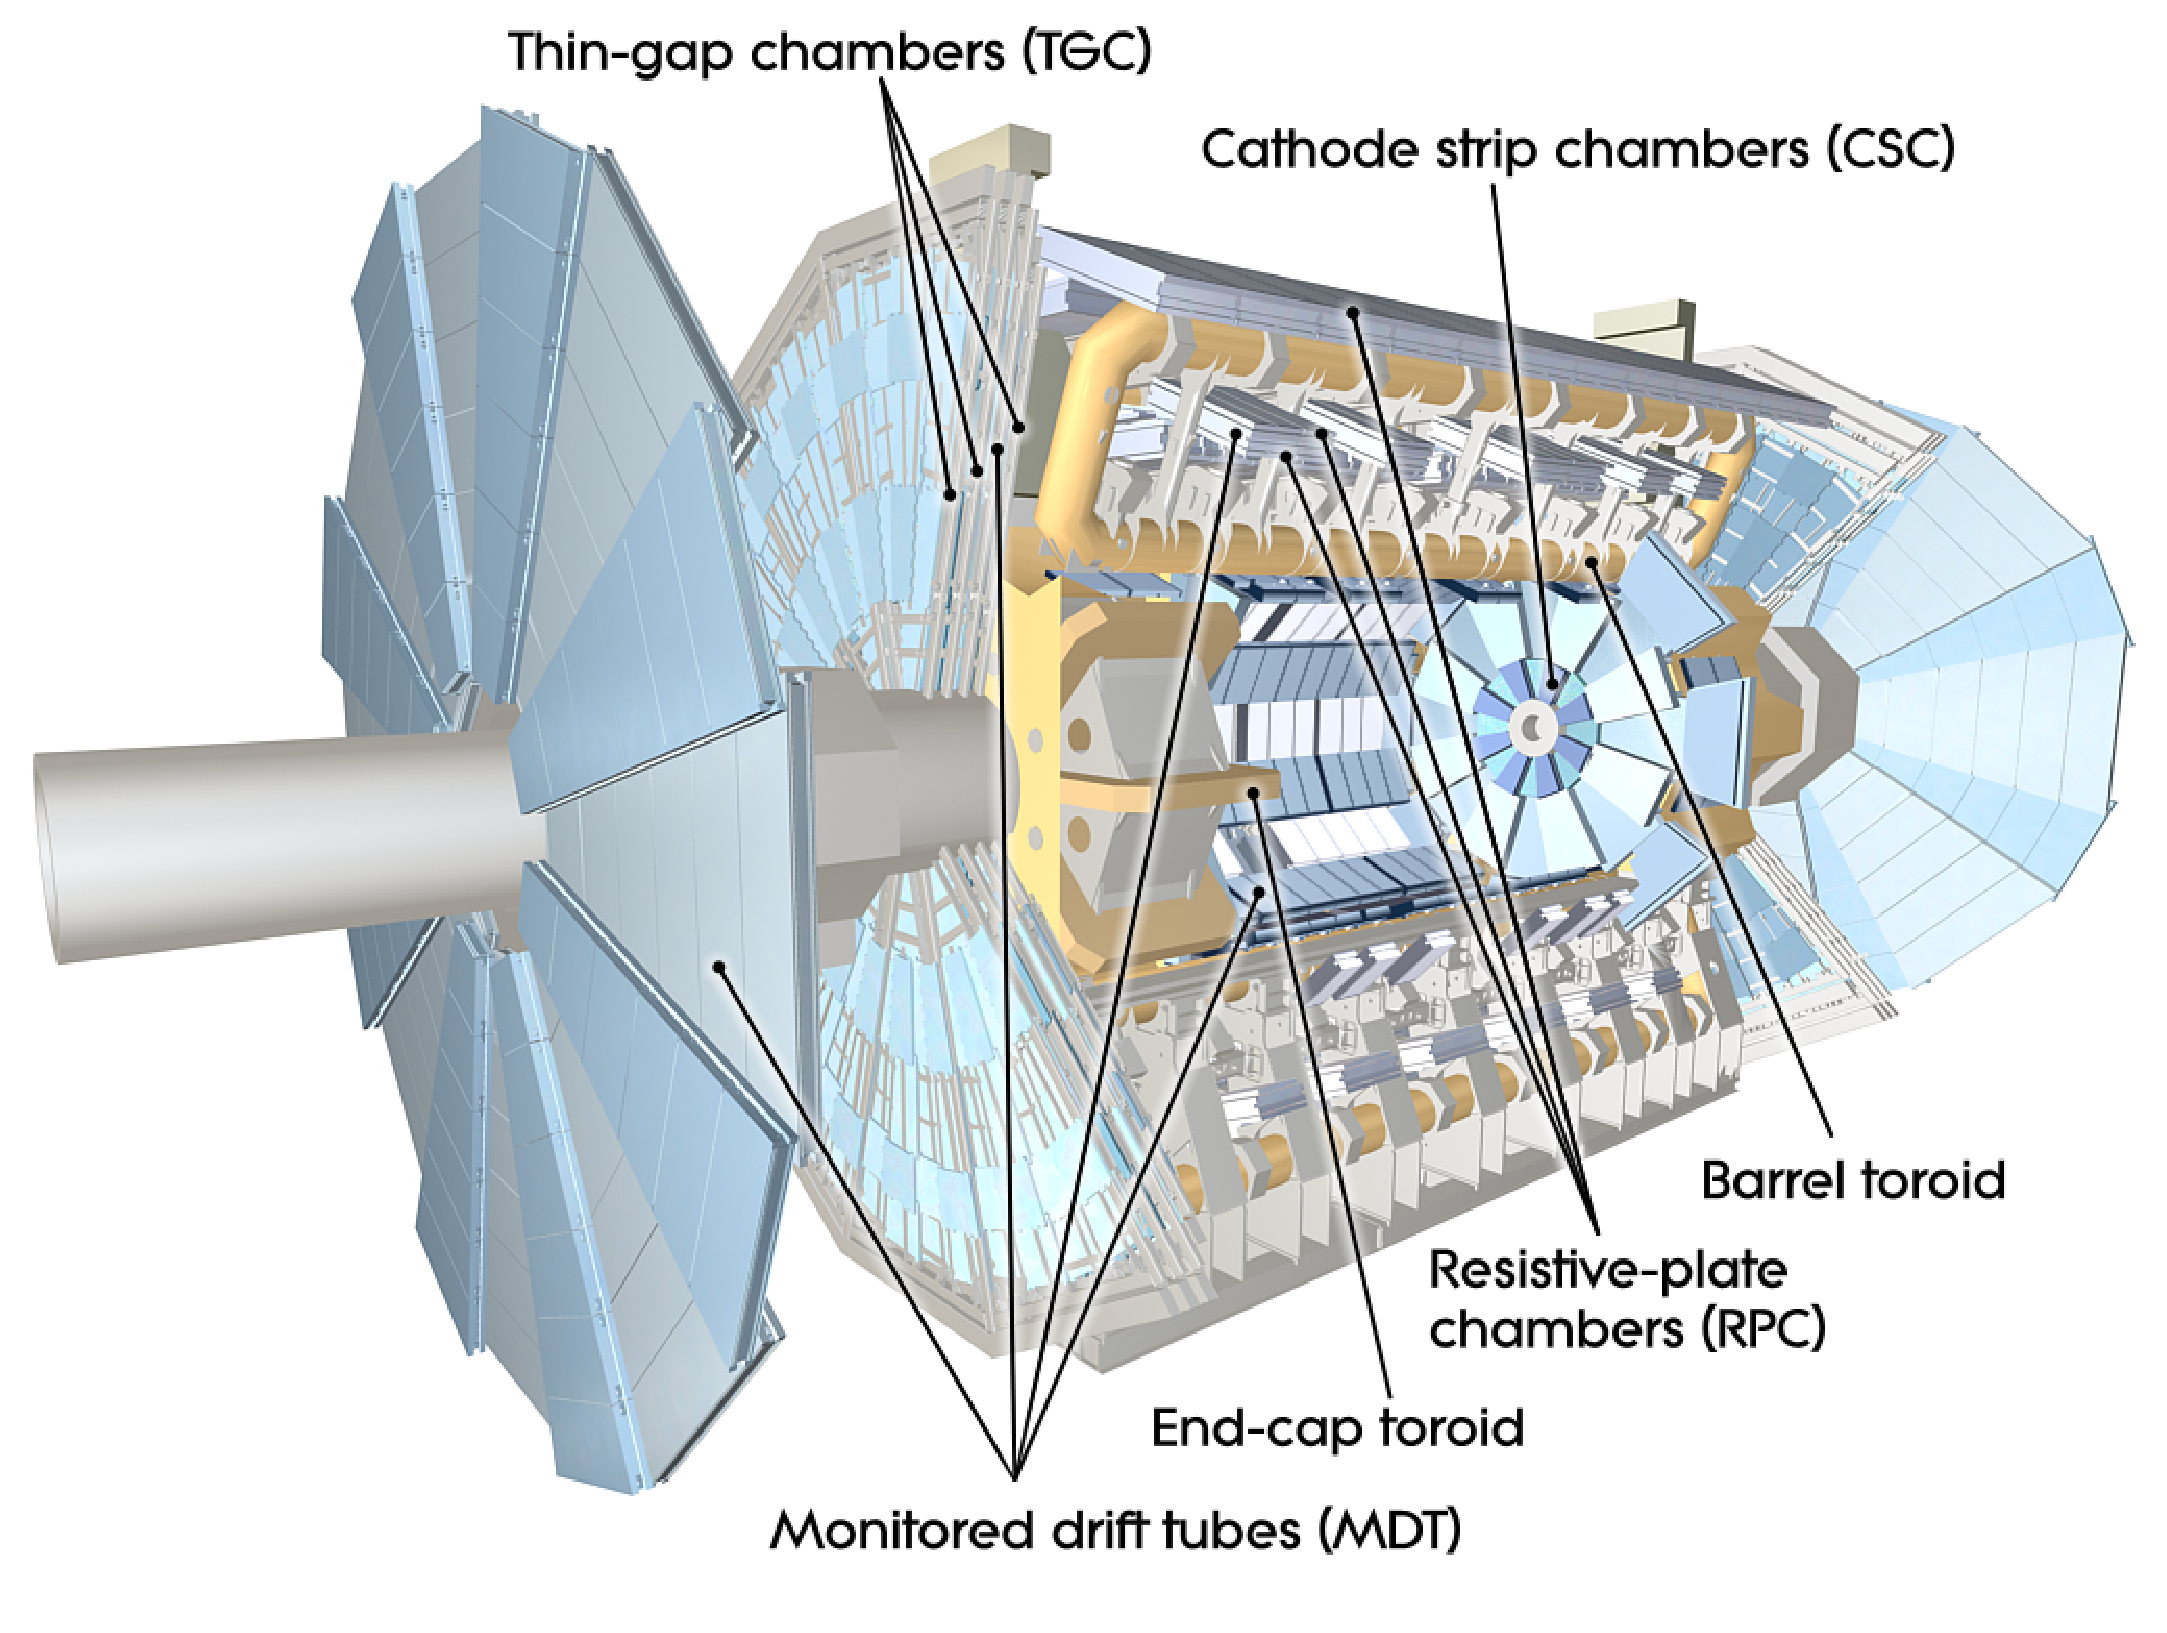
\includegraphics[width=1.0\textwidth]{figures/ATLAS_muon.eps}
\caption{Overview of the ATLAS muon chambers.~\cite{lib:ATLASdet}.}
\label{fig:ATLAS_muon_chambers}}
\end{figure}


The conceptual layout of the muon spectrometer is shown in Fig.~\ref{fig:ATLAS_muon_chambers}. This system is based on the magnetic
deflection of muon tracks in the large superconducting air-core toroid magnets, instrumented with
separate trigger and high-precision tracking chambers. Over the range $|\eta| < 1.4$, magnetic bending
is provided by the large barrel toroid. For $1.6 < |\eta| < 2.7$, muon tracks are bent by two smaller
end-cap magnets inserted into both ends of the barrel toroid. Over the middle region $1.4 < |\eta| < 1.6$, usually referred
to as the transition region, magnetic deflection is provided by a combination of barrel and end-cap
fields. This magnet configuration provides a field which is mostly orthogonal to the muon trajec-
tories, while minimising the degradation of resolution due to multiple scattering. The anticipated
high level of particle flux has had a major impact on the choice and design of the spectrometer instrumentation,
affecting performance parameters such as rate capability, granularity, ageing
properties, and radiation hardness.

In the barrel region, tracks are measured in chambers arranged in three cylindrical layers
around the beam axis; in the transition and end-cap regions, the chambers are installed in planes
perpendicular to the beam, also in three layers.


\section{Magnet system}
\label{sec:ATLAS_magnets}

\begin{figure}
\center{
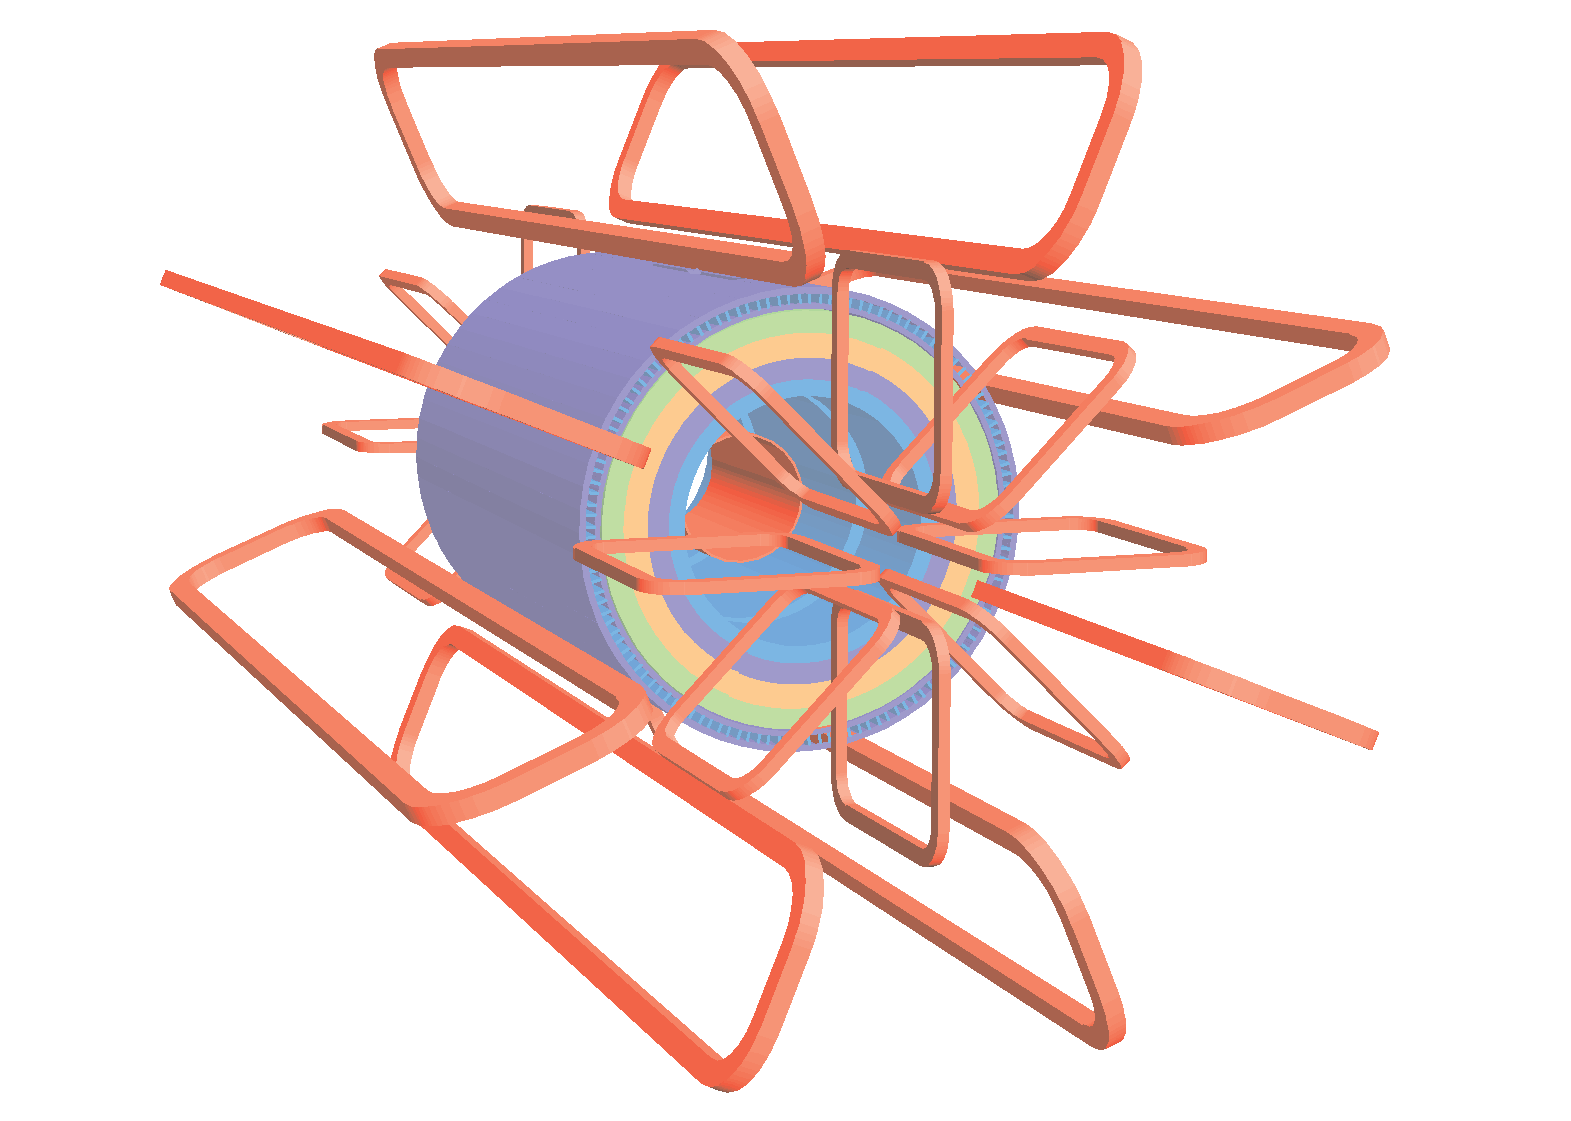
\includegraphics[width=1.0\textwidth]{figures/ATLAS_magnet.eps}
\caption{Overview of the ATLAS magnet system.~\cite{lib:ATLASdet}.}
\label{fig:ATLAS_magnets}}
\end{figure}


ATLAS features a unique hybrid system of four large superconducting magnets. This magnetic
system is 22 m in diameter and 26 m in length, with a stored energy of 1.6 GJ. This systems covers the volume approximately 12,000 m3 (defined as the region in which the field exceeds 50 mT), and engulfs all of the four main layers of detectors (as seen on Fig.~\ref{fig:ATLAS_overview}). The spatial arrangement of the coil windings is shown in Fig.~\ref{fig:ATLAS_magnets}. The ATLAS magnet system consists of:

\begin{itemize}
\item a solenoid, which is aligned on the beam axis and provides a 2 T axial magnetic field for the inner detector, while minimising the radiative thickness in front of the
barrel electromagnetic calorimeter;
\item a barrel toroid and two end-cap toroids, which produce a
toroidal magnetic field of approximately 0.5 T and 1 T for the muon detectors in the central
and end-cap regions, respectively.
\end{itemize}

\section{Online triggers and readout}
\label{sec:ATLAS_trigger}

\begin{figure}
\center{
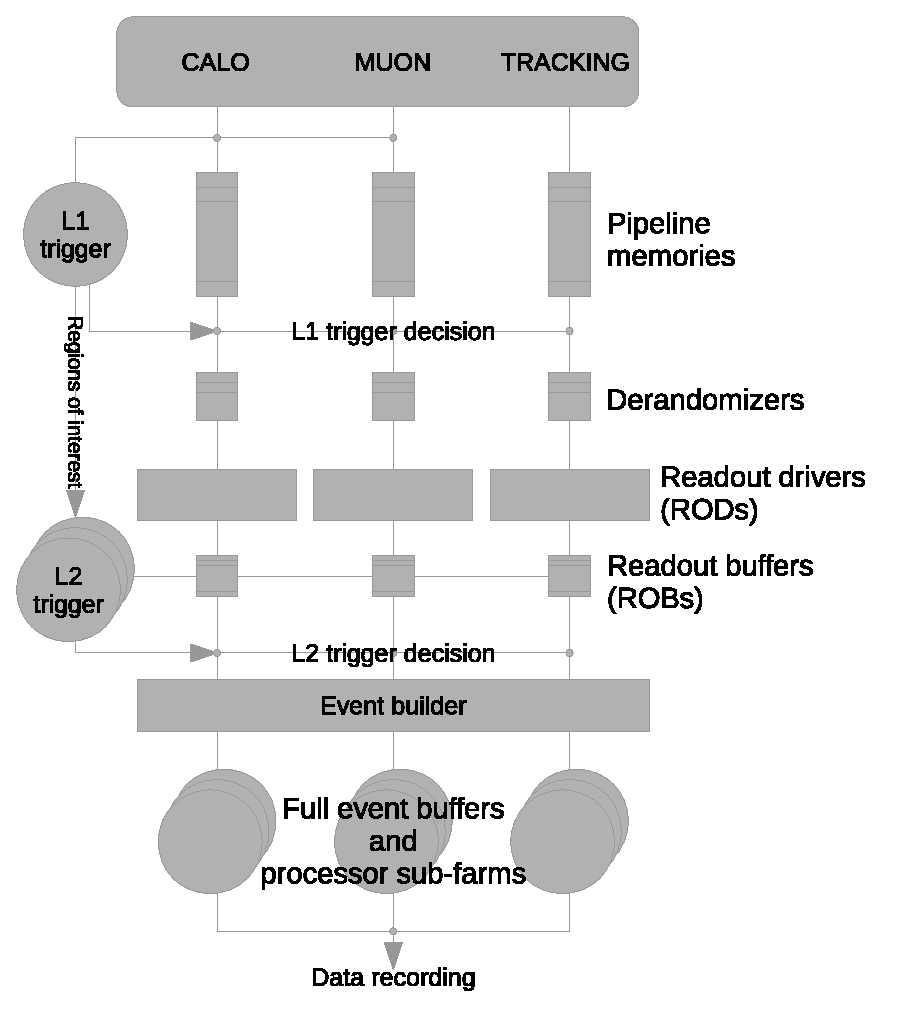
\includegraphics[width=0.7\textwidth]{figures/ATLAS_trigger.eps}
\caption{Diagram of the ATLAS trigger and readout system.}
\label{fig:ATLAS_trigger}}
\end{figure}

The readout system of the ATLAS detector is closely connected with the online trigger system, which consists of two trigger layers (the so-called L1 trigger and L2 trigger), and one event filter~\cite{lib:trigger}. The frequency at which LHC delivers bunch collisions is by design 40 MHz (every 25 ns), although throughout 2011 data taking it was 20 MHz (every 50 ns). It is physically impossible to reconstruct and record every of these 40 millions events per second. And what's more important, only a fraction of these events contain the actual $pp$ collision, so most of the events would be useless even if we managed to record them all. The gradual system of triggers makes an on-the-fly decision whether the event has an actual $pp$ collision or not. The L1 trigger works on the frequency of LHC bunches crossing. This trigger is fully hardware, so it takes a decision in a matter of nanoseconds during the time while the signal from the detectors travels the cables to the readout drivers (RODs). The L1 triggers makes only the rough assumptions about the event, which is it calculates the rough amount of energy deposited in the parts of the calorimeters and muon chambers, and finds so-called "regions of interest" (ROIs), which it passes to the next level trigger, to get a closer look at. The next level trigger is already software based, it is called the L2 trigger, it works on the frequency of 60 KHz and makes its decision while the event is stored in a read-out buffer (ROB). Its output event rate is 5 KHz. The final stage is an event filter which outputs the events at the average rate of 400 Hz. At this rate the events are saved to the output streams. The L2 trigger and the event filter are also collectively called the High Level Trigger (HLT), since they study the event much deeply then the L1 trigger, and work on reconstructed event, rather then the deposited energy, which is what the L1 trigger do. The precision of the L1 trigger is 1 GeV and it only measures the total amount of the deposited $E_{t}$ in the calorimeter towers. The L2 trigger attempts a partial reconstruction of the event in ROIs which are passed down from the L1 trigger as well as track reconstruction, and the event filter does the full event reconstruction in these regions.

The full reconstruction of the filtered event is then done by the large on-site computer farm, and then stored by the use of the data acquisition system (DAQ).

\chapter{Data Samples}
\label{sec:DataSamples}

\begin{table}[ht!]
\centering
\begin{tabular}{ c | cccl } \hline\hline
Period & Run Range & Lumi [$\rm pb^{-1}$] & Max Lumi $\rm [cm^{-2}s^{-1}]$ & Default SE trigger \\ \hline
D & 179710-180481 & & & EF\_e20\_medium \\
E & 180614-180776 & & & EF\_e20\_medium \\
F & 182013-182519 & & & EF\_e20\_medium \\
G & 182726-183462 & & & EF\_e20\_medium \\
H & 183544-184169 & & & EF\_e20\_medium \\
I & 185353-186493 & & & EF\_e20\_medium \\
J & 186516-186755 & & & EF\_e20\_medium \\
K & 186873-187815 & & & EF\_e22\_medium \\
L & 188902-190343 & & & EF\_e22vh\_medium1 \\
M & 190503-191933 & & & EF\_e22vh\_medium1 \\
\hline
\end{tabular}
\caption{The list of 2011 ATLAS data periods used in the Z analysis.}
\label{tab:data}
\end{table}

\chapter{Monte Carlo (MC) Samples}
\label{sec:MCSamples}

In order to analyze the data we use the computer-generated so-called pseudo-data samples using the software that simulates the physical processes that happen in the detector. This pseudo-data is also called "Monte Carlo" or MC and its purpose is to construct the data samples based on the theoretical predictions of our physical model. Ideally, the MC samples should be as close to the real data as possible, allowing us to inspect all the stages of the analysis with a great precision. MC is used for tuning of the reconstruction algorithms (see Sec.~\ref{sec:Reconstruction}), calibration of the calorimeter (see Sec.~\ref{sec:Calibration}), calculation of the efficiencies (see Sec.~\ref{sec:Efficiency}), estimation of the background (see Sec.~\ref{sec:Bkg}), and finally for the comparison of the data to the theoretical predictions (see Sec.~\ref{sec:Results}). Unfortunately, we are unable to recreate the data samples precisely, so some corrections are made by the means of reweightings (see Sec.~\ref{sec:MC_correction}).

The process of generating of the MC samples consists of several stages:
\begin{enumerate}
\item The simulation of the $pp$ collision, which involves the production and the decay of high-energy particles (done by the MC generators, see sec.~\ref{sec:MC_gen}).
\item The simulation of interactions between the high-energy particles and the substance of the detector (done by the Geant4 software~\cite{lib:geant4}, see sec.~\ref{sec:MC_sim_rec}).
\item The simulation of the detector response based on the amount of deposited energy in different parts of the detectors (done by the ATLAS software).
\item The reconstruction process runs the same way as for the genuine data samples, it is fully described in Chapter~\ref{sec:Reconstruction}.
\end{enumerate}
The simulation process takes lots of time, with the most time-consuming process being the simulation of the particles passing through the detector, or even more precise, through the EM-calorimeters, as the calorimeters consist of the very dense materials (e.g. lead and liquid argon) and hence the incoming high-energy particles produce the large showers with the tens of thousands of lower-energy particles. There are several technics used to speed up the process, but most of them produce the different result from the standard not-optimized simulation, which makes them unusable for many types of analysis (including \Zee). The only technology which gives the result close enough to the standard simulation to be enabled for all analysis samples by default is the Frozen Showers, which will be fully described in sec.~\ref{sec:MC_FS}.

\section{MC generators used in ATLAS experiment}
\label{sec:MC_gen}

The first stage of the MC production is the simulation of the $pp$ collision itself. The simulation of this process is based on the standard model, and tries to account for every significant aspect of it. The core of the simulation is the calculation of the matrix element (ME) of the $pp$ interaction, which can be done in different orders. The simplest case is the leading order (LO), which in case of the $\Zee$ is the bare Drell-Yan diagram, with no loops or extra legs. The simulations in the leading order are not precise, and generally the next to leading order (NLO) or next to next to leading order (NNLO) are used instead, with one or two extra loops/legs respectively. The calculation of the matrix element in higher orders is very complex, and in order to increase the precision of the simulation the additional particles are simulated outside of the ME. Additional QCD particles are generated using the "parton shower" (PS) technique, which is to simulate the QCD radiation on every parton independently, using the formulas not unlike the ME. The PS technique is widely adopted and used in every MC generator. Additional QED radiation is generated in a similar way by the independent package named "Photos"~\cite{lib:photos}, with the similar technique. This package can be used in conjunction with other MC generators.

Here is the list of the most noticeable MC generators used in ATLAS analyses:
\begin{itemize}
\item \Herwig~\cite{lib:MC_herwig} is a general-purpose event generator for high-energy processes, with particular emphasis on the detailed simulation of QCD parton showers. The program provides a full simulation of hard lepton-lepton, lepton-hadron and hadron-hadron scattering and soft hadron-hadron collisions in a single package, and has the following special features:
\begin{itemize}
\item Initial- and final-state QCD jet evolution with soft gluon in terference taken into account via angular ordering.
\item Color coherence of (initial and final) partons in all hard subprocesses, including the production and decay of heavy quarks and supersymmetric particles.
\item Azimuthal correlations within and between jets due to gluon interference and polarization.
\item A cluster model for jet hadronization based on non-perturbative gluon splitting, and a similar cluster model for soft and underlying hadronic events.
\item A space-time picture of event development, from parton showers to hadronic decays, with an optional color rearrangement model based on space-time structure.
\end{itemize}
In MC11c \Herwig\ is used to provide the parton showering for other generators.

\item \Pythia~\cite{lib:MC_pythia} is a generator with the objective to provide as accurate as possible a representation of event properties in a wide range of reactions, within and beyond the Standard Model, with emphasis on those where strong interactions play a role, directly or indirectly, and therefore multihadronic final states are produced. The physics is then not understood well enough to give an exact description, instead the program has to be based on a combination of analytical results and various QCD-based models.

\item \Powheg~\cite{lib:MC_powheg} is a hard event generator for heavy quark production in hadronic collisions. It is accurate at the next-to-leading order in QCD, and it can be interfaced to Shower Monte Carlo programs like \Herwig\ and \Pythia, in such a way that both the leading logarithmic accuracy of the shower and the NLO accuracy are maintained in the output. This generator is the main MC generator used in 2011 analyses.

\item \Mcatnlo~\cite{lib:MC_mcatnlo} is a practical implementation, based upon the Fortran \Herwig\ and \Herwigpp\ event generators, of the \Mcatnlo\ formalism, which allows one to incorporate NLO QCD matrix elements consistently into a parton shower framework.

\end{itemize}

\subsection{Signal MC}

The part of Monte Carlo simulation which represents \Zee\ events is called "signal MC". \tbu uses
As well as the standard model itself, the MC generators have parameters which can't be theoretically predicted, and should be found empirically. This process is called "MC tuning", and is done separately for every experiment, because the tune which will describe well one experiment won't fit for other. The tunes used in ATLAS are described in~\cite{lib:MC_tune1, lib:MC_tune2}.

The other important part of MC customization is the PDF set. PDF stands for "parton distribution function". It is a model that describes the energy distribution between quarks inside the proton. There are several PDF sets calculated based on the data from different experiments. The sets are distributed with the LHAPDF software~\cite{lib:lhapdf}, which represents the full compendium of PDF sets calculated and validated by this time. The biggest contributions to the PDF collection were done by the Tevatron and HERA experiments. The PDF sets used in the current analyses are dicribed in~\cite{lib:MC_pdfct10, lib:MC_pdfcteq6l1}.

\subsection{Background MC}

The part of Monte Carlo simulation which represents different EM processes which can be misinterpreted as \Zee\ is called "background MC". We use seven different types of backgrond MCs.
\begin{itemize}
\item \Wenu, the decay of $W$ boson into electron and neutrino. Can be misinterpreted as $Z$ decay if another electron is reconstructed in the same event, most notably, when a jet is misinterpreted as an electron (a "fake electron").
\item \Wtau, the decay of $W$ boson into tau and neutrino. Can be misinterpreted if tau decays into electron, and another unrelated electron is reconstructed as in the previous case.
\item \Ztau, the decay of $Z$ boson into two taus. Can be misinterpreted if at least one tau decays into electron, and another electron is reconstructed. The case of both tau decaying into electrons and $Z$ boson constructed from them is is also possible, since the mass window is wide enough for that.
\item \ttbar\ events, which have lots of decay modes, and thus can be misinterpreted as almost anything, including \Zee. The most common case is \ttbar\ decaying into $W^{+}W^{-}\antibar{b}$, and thus falling into the $WW$ category.
\item $WW$, can be misinterpreted if both bosons decay into $e\nu$.
\item $WZ$, and $ZZ$ events. In our analysis we filter such events, and thus misinterpretation of e.g. $WZ$ event as \Zee\ event is a background event for us.
\end{itemize}

\section{MC production chain}
\label{sec:MC_sim_rec}

The output of the MC generators consists of the set of the final-state particles, which in turn are passed to the ATLAS MC production chain. This chain consist of three main stages, namely: the simulation, digitization and the reconstruction (see Fig.~\ref{fig:MC_gen}).

Although the whole process of the production of the MC samples can be considered as "simulation", in this context "the simulation process" refers to the particular stage of the whole production chain: the simulation of the propagation of the high-energy particles through the matter of the detector. It is done using the Geant4 software and the highly-accurate 3D model of the detector. The simulation in Geant4 is done as a discrete step-by-step process, with the length of the step being calculated dynamically for each particle, based on particle energy and the physical processes that happen to that particle. Because of that the simulation of the particles in vacuum takes much less time than in heavy matter. That is the reason why the majority of the simulation time is spent in calorimeters: they are built of the densest material there is in explicit purpose to stop as many particles as possible.

The output of the simulation stage is "hits", the 4D vertexes of energy deposits in sensitive areas of the detectors. The next stage is to simulate the work of the detector itself, or to convert the energy deposits into detector response, which are usually voltages on the read-out channels. This process is called "digitization", because its output is "digits" which the read-out channels provide. During this stage all features of the detector logic are simulated (e.g. electric noises or channel-dependent variations). This is done by the internal ATLAS digitization software, and because it requires an intimate knowledge of every particular sub-detector, parts of it are maintained by separate groups related to the respective sub-detectors.

The last step in the production chain is the same for both MC and genuine data samples, as the digitization process aims to provide the same data as we get from the detector during production runs. During this step the responses from the detector are reconstructed into physical objects, which is done in two steps. First step is more on the technical side, during which the response from the trackers is reconstructed into tracks and the response from the calorimeters is reconstructed into clusters. The second stage is physical and depends on the analysis. During this stage the tracks and clusters are combined into the physical particles. The flavors of this stage of reconstruction include e/gamma, jet/EtMiss/tau, b tagging and muon. $\Zee$ analysis uses the first: e/gamma flavored reconstruction. This process is done using the internal ATLAS reconstruction software. More on the reconstruction process with respect to the real data from the detector is in Sec.~\ref{sec:Reconstruction}.

The result of the reconstruction is the data stored in the special format called AOD (Analysis Data Object), which is also developed internally by ATLAS. AODs can be read by the ATLAS analysis framework, which gives easy access to all reconstructed objects.

\begin{figure}
\center{
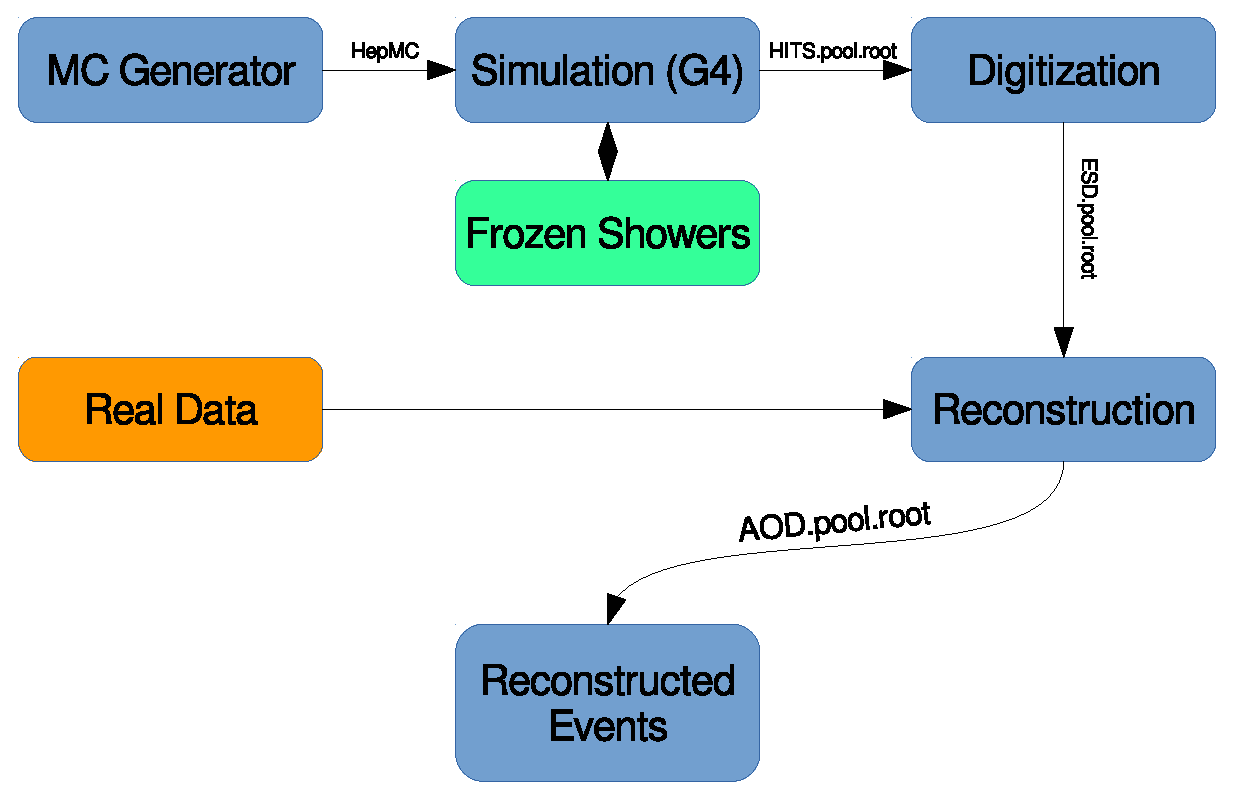
\includegraphics[width=0.7\textwidth]{figures/MC_production_chain.eps}
\caption{Diagram of the ATLAS MC production chain}
\label{fig:MC_gen}}
\end{figure}

\subsection{Frozen Showers}
\label{sec:MC_FS}
The frozen showers system (FS) is a system that is designed to speed up the geant4 simulation process inside the EM calorimeters. The main principle of FS is to substitute the low-energy particles with the EM-showers, which are pre-simulated and stored in the libraries (see Fig.~\ref{fig:MC_FS_method}). These libraries must be generated in advance for each calorimeter and for each type of particles which is needed to be fast-simulated during the production simulation. The generation process consists mostly of the simulating of the low-energy particles and saving the information about every energy deposition this particle made. The array of these deposits or "hits" passes through several post-processing procedures in order to reduce its size, and becomes a "shower".

\begin{figure}
\center{
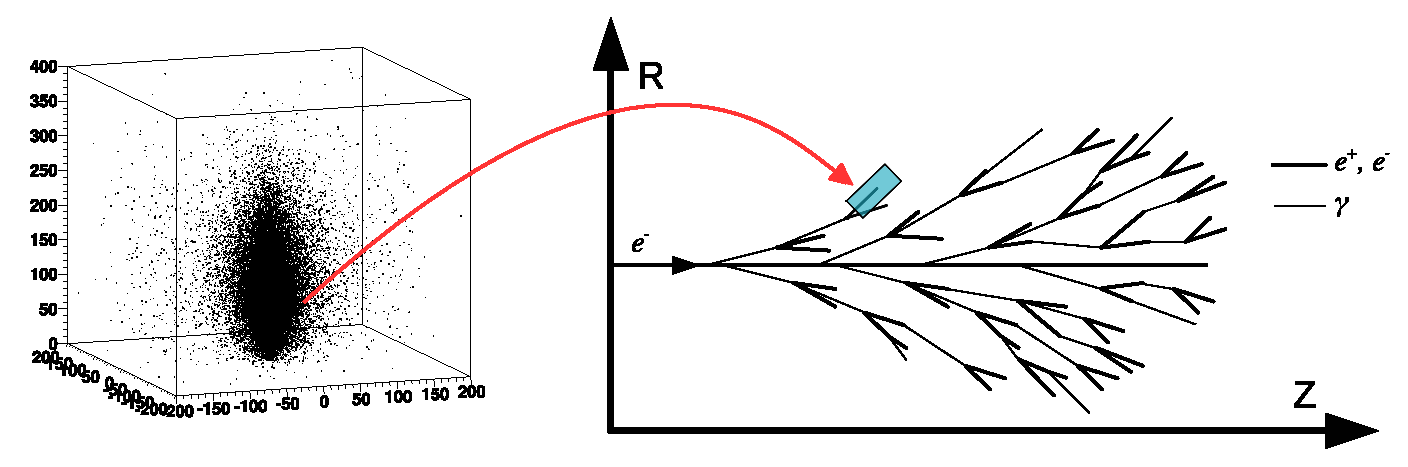
\includegraphics[width=1.0\textwidth]{figures/MC_FS_method.eps}
\caption{Diagram showing the shower substitution of the low-energy particle, during the high-energy particle simulation.}
\label{fig:MC_FS_method}}
\end{figure}

The generation of the shower library is thus a preparatory procedure, which needs to be done every time when something is changed in the geant4 simulation process. The examples are the change of the geant4 version used, or the change in the detector geometry. Usually these changes applied between the MC campaigns, which means that the new set of libraries needs to be generated for each campaign. In order to improve results of FS-enabled simulation the libraries are then tuned: the shape and the energy response of the stored showers are slightly changed to provide the needed changes in the resulting simulation.

The processes of the library generation (and tuning) and the production use FS system would be described separately in the two following sections.

\subsubsection{FS library generation}
\label{sec:MC_FS_gen}

The library is the set of the showers simulated from the low-energy particles of the same (needed) type. The library should be able to provide the shower for any particle of this type within the determent energy bounds and inside the corresponding sub-detector. Thus, the showers populating the library should also be generated with all the possible energies and in all of the sub-detectors volume. To do this we need to generate the low-energy particles (as during the generation stage described in sec.~\ref{sec:MC_gen}) with different energies and different vertexes that covers continuously both volume and energy range.

The easiest way to do it is to use a particles gun: a tool that can create a particle with arbitrary type, momentum and vertex. This way we will get a library uniformly populated by libraries in every part of its kinematic space. This approach has two major disadvantages. First, it reduces the quality of the simulation. As we can't match all of the particle parameters while searching for the suitable shower within the library (it will take too much time time and require the libraries of enormous sizes), we disregard some of them and introduce large bins on some others. Because of that the matched shower can have substantially different properties then the required particle. The second problem is the oversized library. During the production simulations the libraries from some part of the kinematic space (e.g. with the lowest energy of $0-10 MeV$ as opposed to $500-1000 MeV$) are requested more often than others. This makes some showers overused and some other underused, worsening the results of the simulation and introducing the redundant memory footprint.

The better way to handle this is to generate the library using the process similar to the usual MC production chain. It is called a two-staged library generation. The first stage is to conduct the normal simulation of the MC samples, but on much lesser scale, only hundreds are required. During the simulation, every time when the low-energy particle is requested to be fast-simulated using FS, the parameters of this low-energy particle are saved as a starting point for the shower. As the starting points tend to be clustered very tightly around the track of the initial high-energy particle, only the fracture of the initial starting points is used for library generation in order to rarify them and get a more even coverage of the detector's volume. The sample coverage of the all EM calorimeters in ATLAS detector can be seen in fig.~\ref{fig:MC_FS_stpoints}. The second stage is the simulation itself. During this stage the starting points are taken one-by-one and simulated using the standard simulation infrastructure, producing the showers, which in turn go to the final library. The density distribution of the simulated hits within the shower can be seen in fig.~\ref{fig:MC_FS_shower}

\begin{figure}
\center{
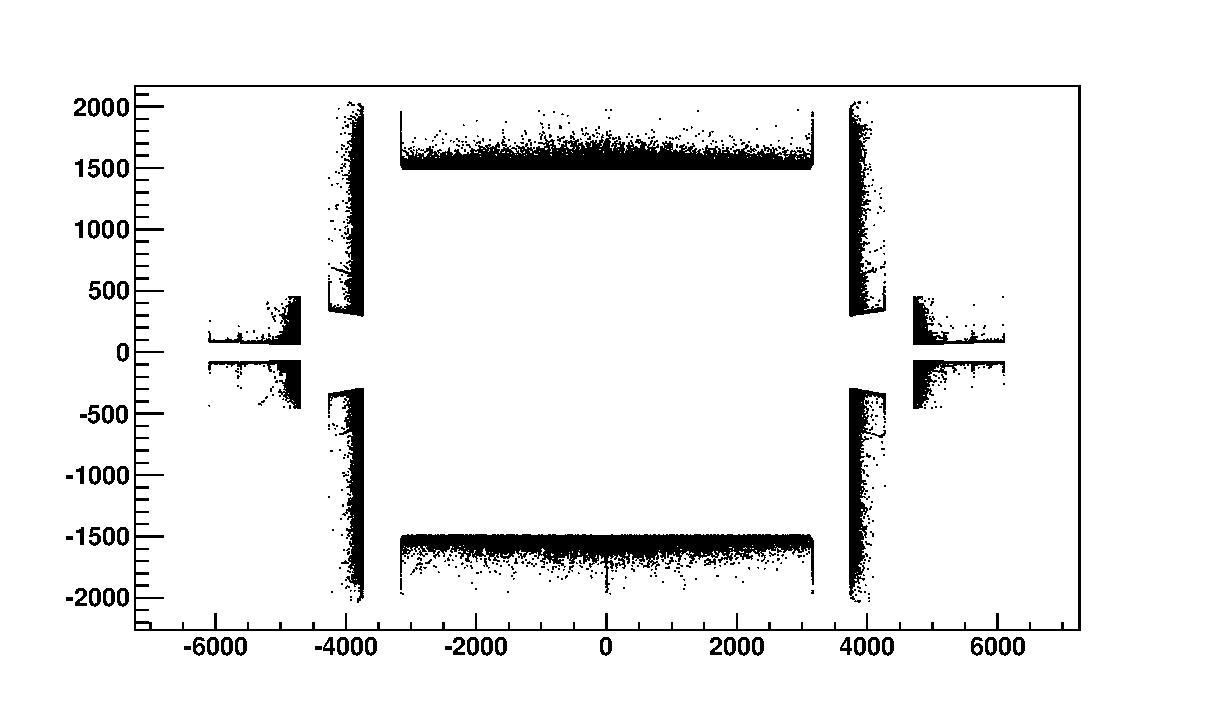
\includegraphics[width=1.0\textwidth]{figures/MC_FS_stpoints.eps}
\caption{The first stage of the 2-staged library production: FS starting point generation}
\label{fig:MC_FS_stpoints}}
\end{figure}

\begin{figure}
\center{
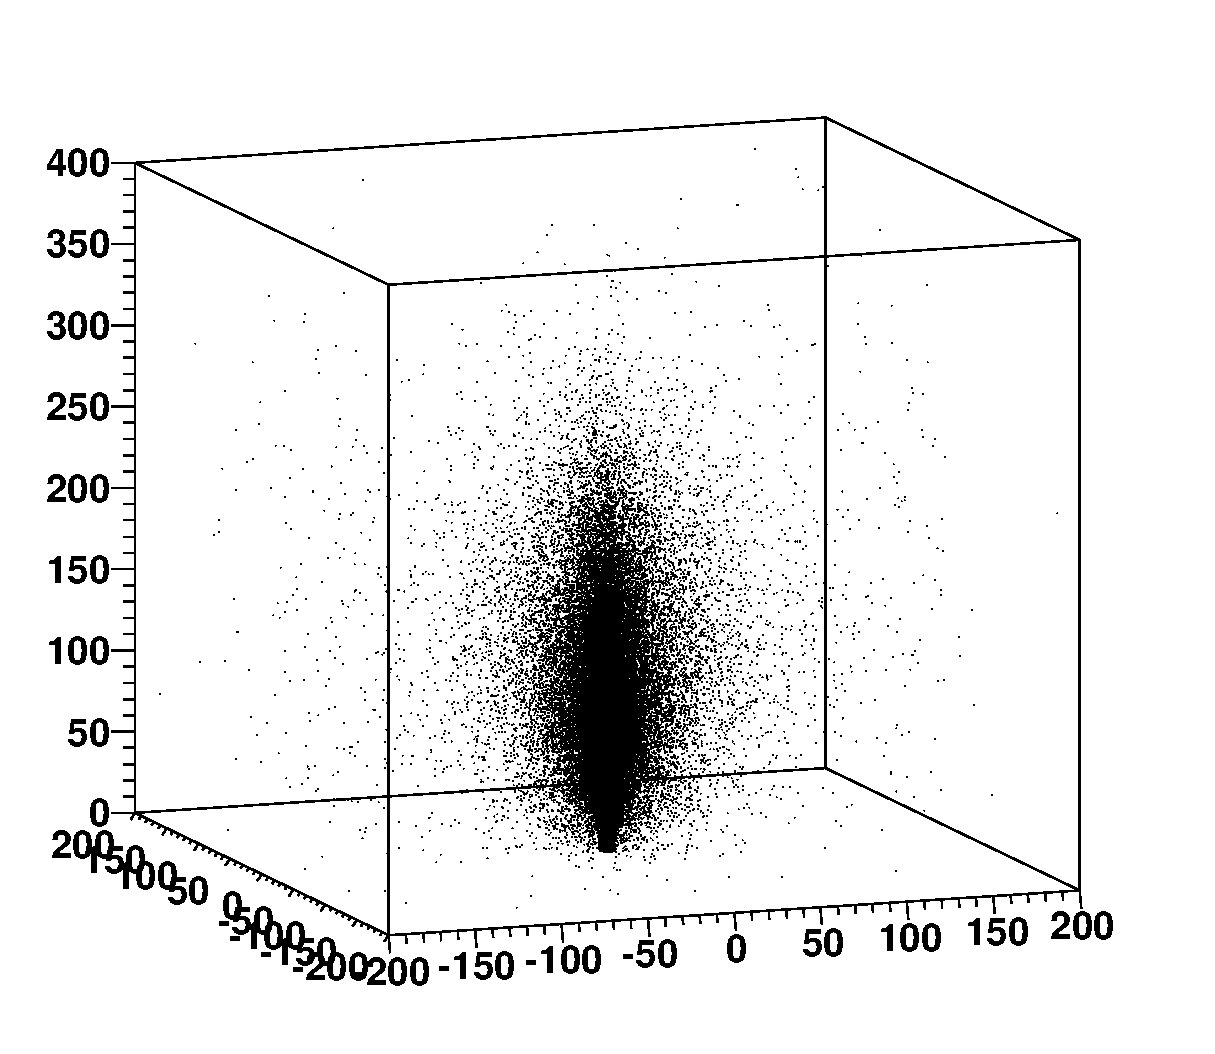
\includegraphics[width=0.75\textwidth]{figures/MC_FS_shower.eps}
\caption{The second stage of the 2-staged library production: the simulation of the shower}
\label{fig:MC_FS_shower}}
\end{figure}

This way of library generation solves all the problems mentioned above. The bin population problem does not occur because we produce the showers based on the physical MC samples, and the resulting size of each kinematic bin is in direct dependence of the number of times this bin is used. This allows to reduce the size of the library and yet make a bigger diversity.

The post-processing stage consists of merging of the adjacent hits and of removing the far-standing hits that won't contribute to the reconstructed cluster anyway. Also, during this stage the size of the shower is calculated. It is used for containment check during the production (which is when we check if the shower we are about to substitute the particle with is fully contained within the target detector).

The tuning of the library can then be applied manually in order to make the results the FS simulation closer to the standard simulation (also called "full simulation") or the data. As this is a process that can't be (as of yet) done automatically, it requires lots of time and effort.

\subsubsection{FS production use}
\label{sec:MC_FS_prod}

During the production run the simulation software checks constantly if any particle agree with the fast-simulation criteria, which is the energy range (should be low enough) and the sub-detector containment (the particle should be far enough from the edges of the sub-detector volume for shower to fit within). The containment check is energy-dependent, because the sizes of the showers grow with energy, and the more energetic particles should be further from the edges in order for shower to fit.

When the particle with the proper parameters is found, it is then removed from the simulation and replaced with the shower. Before the deposition, the shower is scaled to fully correspond to the particle in energy.

\begin{figure}
\center{
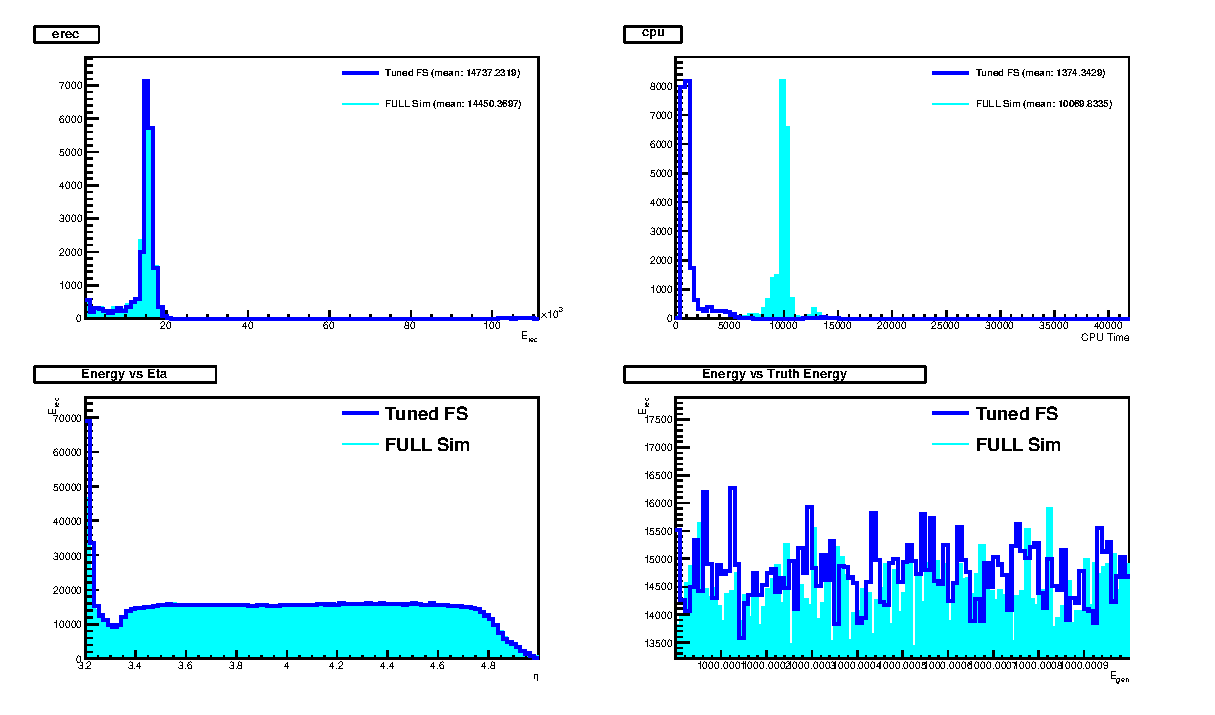
\includegraphics[width=1.0\textwidth]{figures/MC_FS_speedup.eps}
\caption{The simulation result for single electrons with energy 1000~GeV. CPU speed-up can be seen in top right. \tbu A BETTER PLOT}
\label{fig:MC_FS_speedup}}
\end{figure}

For the MC11c and MC11d campaigns, the data from which is used in this analysis, frozen showers system was enabled by default in FCAL. Several studies showed that the differences introduced by the FS is negligible compared to the differences between MC and data, while the simulation speedup was about 25\%. The smallness of the errors introduced by the FS compared to other fast simulation methods (most notably - FastCaloSim) leaded to the misunderstanding, when the simulation with the FS system enabled was called "full simulation" as opposed to other, less precise but faster methods, which were called "fast simulation". In this terminology, all of the MC samples used in this analysis are full simulations.

The sample comparison of the default, non-accelerated MC samples with the samples with enabled frozen showers can be seen in Fig.~\ref{fig:MC_FS_speedup}. It can be seen that the speed-up is significant, while the results remain the same.

\section{MC samples used in analysis}
\label{sec:MC_periods}

During this analysis the MC samples from both MC11c and MC11d campaigns were used. The "d" is chronologically the fourth sample produced for the 2011 data, and the "c" is the third. The decision to make new samples is usually made when some errors in GEANT software or in ATLAS geometry are discovered. The latest "d" sample fixes all such known errors, which affected the electron performance in various cases. The "d" is thus used in cases where the electron performance is important. The main generator used for both signal and background was \Powheg\ with the parton showering provided by \Pythia. The cross-check was done by the same \Powheg\ with the PS done by \Herwig\, and by \Mcatnlo\ also with the \Herwig-provided showers. For the
\Mcatnlo\ and \Powheg\ matrix element calculations the \pdfCteq\ PDF set is used, while showering was performed with \pdfCteql PDF. The list of MC signal periods that was used can be found in Tab.~\ref{tab:MC_periods}, the periods for MC background events are in Tab.~\ref{tab:MC_bg}.

\begin{table}
  \begin{center}
    \begin{tabular}{@{ } l @{ }| r @ { } | @{ } r @{ } | @{ }r@{}}
      \hline
      \hline
      Data set & Generator& $\sigma{\cdot}\text{BR}{\cdot}\epsilon_{filter}$ [nb] & $N_{evt}\,[10^6]$\\
      \hline

      108303$^{\mathrm{d}}$ &   \Powheg\Pythia & 1.006 (5\%) & 20\\

      126006 &   \Powheg \Herwig & 1.006 (5\%) & 10\\

      106087 \&~129913 & \Mcatnlo & 0.990 (5\%) & 5+5\\

      147770 & \Sherpa & 1.070 (5%) & 10 \\

      \hline
    \end{tabular}
    \caption{Signal Monte Carlo samples. The sample marked with $^{\mathrm{d}}$ was taken from the MC11d campaign, the others are from the MC11c.}
    \label{tab:MC_periods}
  \end{center}
\end{table}

\begin{table}
  \begin{center}
    \begin{tabular}{@{} l @ { }|@{ } l @{ }| r @ { } | @{ } r @{ } | @{ }r@{}}
      \hline
      \hline
      Process & Data set & Generator & $\sigma{\cdot}\text{BR}{\cdot}\epsilon_{filter}$ [nb] & $N_{evt}\,[10^6]$\\
      \hline

      \Wplusenu       & 108297$^{\mathrm{d}}$  &  \Powheg\Pythia  &
      6.160 (5\%) & 23 \\
      \Wminusenu & 108300$^{\mathrm{d}}$  &  \Powheg\Pythia &
      4.300 (5\%) & 17 \\
      \Wplusenu       & 113186 &  \Powheg\Herwig  &
      6.160 (5\%) & 16 \\
      \Wminusenu & 113184 &  \Powheg\Herwig &
      4.300 (5\%) & 12 \\
      \Wplusenu       & 106080 & \Mcatnlo &
      6.160 (5\%) & 16 \\
      \Wminusenu & 106081 & \Mcatnlo &
      4.300 (5\%) & 12 \\

      \hline

      \Wtau\ Np0   &  107700 &  \Alpgen\Herwig\ & 8.285 (5\%) & 3.4 \\
      \Wtau\ Np1   &  107701 &  \Alpgen\Herwig\ & 1.560 (5\%) & 2.5 \\
      \Wtau\ Np2   &  107702 &  \Alpgen\Herwig\ & 0.452 (5\%) & 3.8 \\
      \Wtau\ Np3   &  107703 &  \Alpgen\Herwig\ & 0.122 (5\%) & 1 \\
      \Wtau\ Np4   &  107704 &  \Alpgen\Herwig\ & 0.0307 (5\%) & 0.25 \\
      \Wtau\ Np5   &  107705 &  \Alpgen\Herwig\ & 0.00835 (5\%) & 0.07 \\
      \Wtau        &  107054 &  \Pythia\        & 10.460 (5\%) & 1 \\
      \Wplusenu & 147412$^{\mathrm{d}}$  &  \Powheg\Pythiaeight  &
      6.160 $\cdot$ 0.1510 (5\%) & 15 \\
      \Wminusenu & 147415$^{\mathrm{d}}$  &  \Powheg\Pythiaeight  &
      4.300 $\cdot$ 0.1404 (5\%) & 10 \\
      \hline

      \Ztau\ Np0  &  107670 &  \Alpgen\Herwig\  & 0.834 (5\%) & 6.6 \\
      \Ztau\ Np1  &  107671 &  \Alpgen\Herwig\  & 0.168 (5\%) & 1.3 \\
      \Ztau\ Np2  &  107672 &  \Alpgen\Herwig\  & 0.0508 (5\%) & 0.81 \\
      \Ztau\ Np3  &  107673 &  \Alpgen\Herwig\  & 0.0140 (5\%) & 0.22 \\
      \Ztau\ Np4  &  107674 &  \Alpgen\Herwig\  & 0.00355 (5\%) & 0.06 \\
      \Ztau\ Np5  &  107675 &  \Alpgen\Herwig\  & 0.00093 (5\%) & 0.02 \\
      \Ztau\      &  106052 &  \Pythia\         & 0.990 (5\%) & 3\\
      \Ztau & 147418$^{\mathrm{d}}$ &   \Powheg\Pythiaeight   &
      0.990 $\cdot$ 0.263 (5\%) & 6\\
      \hline

      \ggee & 129652 & \Pythiaeight & $2.41\cdot 10^{-3} \cdot 0.7$ (40\%) & 0.5\\

      \hline

      \ttbar  & 105200$^{\mathrm{d}}$ & \Mcatnlo & $0.1773\, (6.2\%) \cdot \, 0.555$ & 1.5\\

      \hline

      $WW$ & 105985$^{\mathrm{d}}$ & \Herwig & 44.9 $\cdot$ 0.389 $\cdot 10^{-3}$ (7\%) & 1.5 \\
      $WZ$ & 105987$^{\mathrm{d}}$ & \Herwig & 18.5 $\cdot$ 0.310 $\cdot 10^{-3}$ (7\%) & 1 \\
      $ZZ$ & 105986$^{\mathrm{d}}$ & \Herwig & 6.02 $\cdot$ 0.212 $\cdot 10^{-3}$ (7\%) &
      0.25 \\

      \hline
    \end{tabular}
    \caption{ Background Monte Carlo samples. The samples marked with $^{\mathrm{d}}$ were taken from the MC11d campaign, the others are from the MC11c. }
    \label{tab:MC_bg}
  \end{center}
\end{table}

\section{Reweightings}
\label{sec:MC_correction}

The MC samples have a number of known shortcomings, and some data distributions are not described well. To fix this we apply reweightings based on MC/data comparisons at the reconstruction levels, different MCs comparisons on the generation (truth) level, or using the other ATLAS analyses. The weights are applied based on the truth information and are validated using the closure tests. The list of corrections is this:

\begin{itemize}
\item \textbf{Pileup Reweighting} is based on the $\mu$ variable and aims to equalize the amount of pileup in MC and data. This is done using the \textit{PileupReweighting} tool~\cite{lib:pileuptool, lib:pileupscale}.
\item \textbf{Vertex Spread in $z$ Reweighting} is based on the $z$ component of the vertex and aims to decrease the spread of the beam spot in $z$-direction of MC, which is significantly smaller in data (for data $\sigma_z \approx 56$mm, while for narrow beam spot MC sample $\sigma_z = 75$mm and for wide beam spot $\sigma_z = 90$mm). The \texttt{VertexPositionReweightTool} is used for that. The effect of this correction can be seen in Fig.~\ref{fig:MC_zvtx}.
\item \textbf{$Z$ Boson $p_T$ Reweighting} is applied to the $p_T$ distribution of the $Z$ bosons, which doesn't describe the data well in the MC signal generators used for this analysis. The results from ATLAS $Z$ $\phi^*$ and $\pt$ analyses~\cite{lib:Zphistar} were used for it, and it was done using the \texttt{BosonPtReweightingTool}.
\item \textbf{$Z$ Boson Line Shape Reweighting} is the reweightings aimed to fix the fundamental shortcomings of the MC generators caused by the electroweak order not being high enough. This reweighting is done using the \texttt{LineShapeTool}. See~\cite{lib:lineshape} for details.
\end{itemize}

\begin{figure}
\center{
\subfigure[$z_{vtx}$ weights] {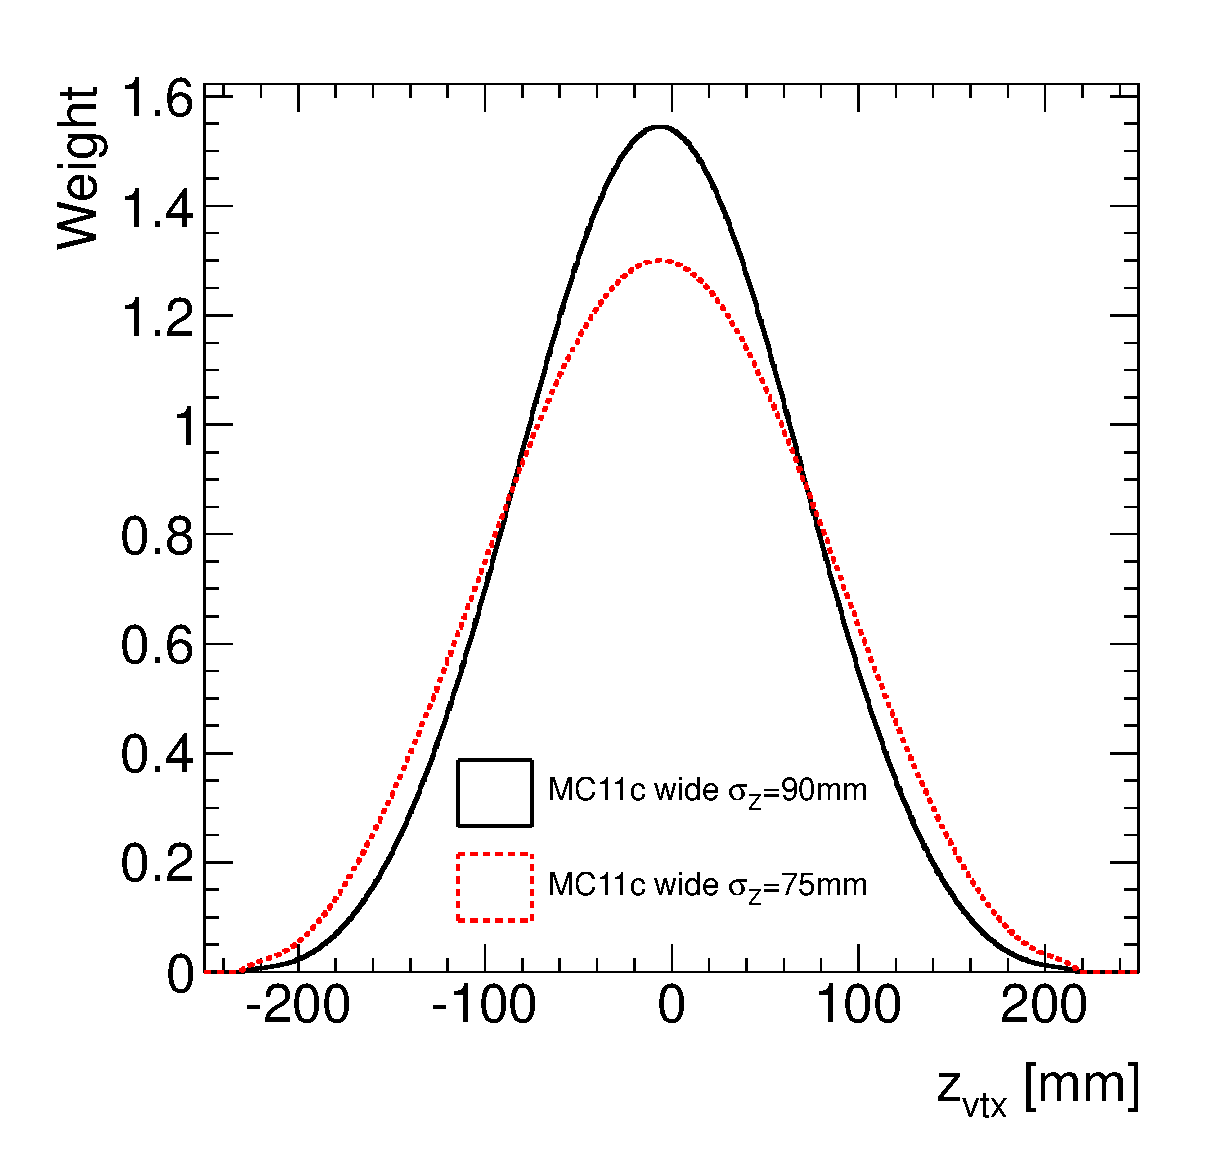
\includegraphics[width=0.32\textwidth]{figures/MCrew_zvtx_weights.eps}}
\subfigure[Before $z_{vtx}$ reweight] {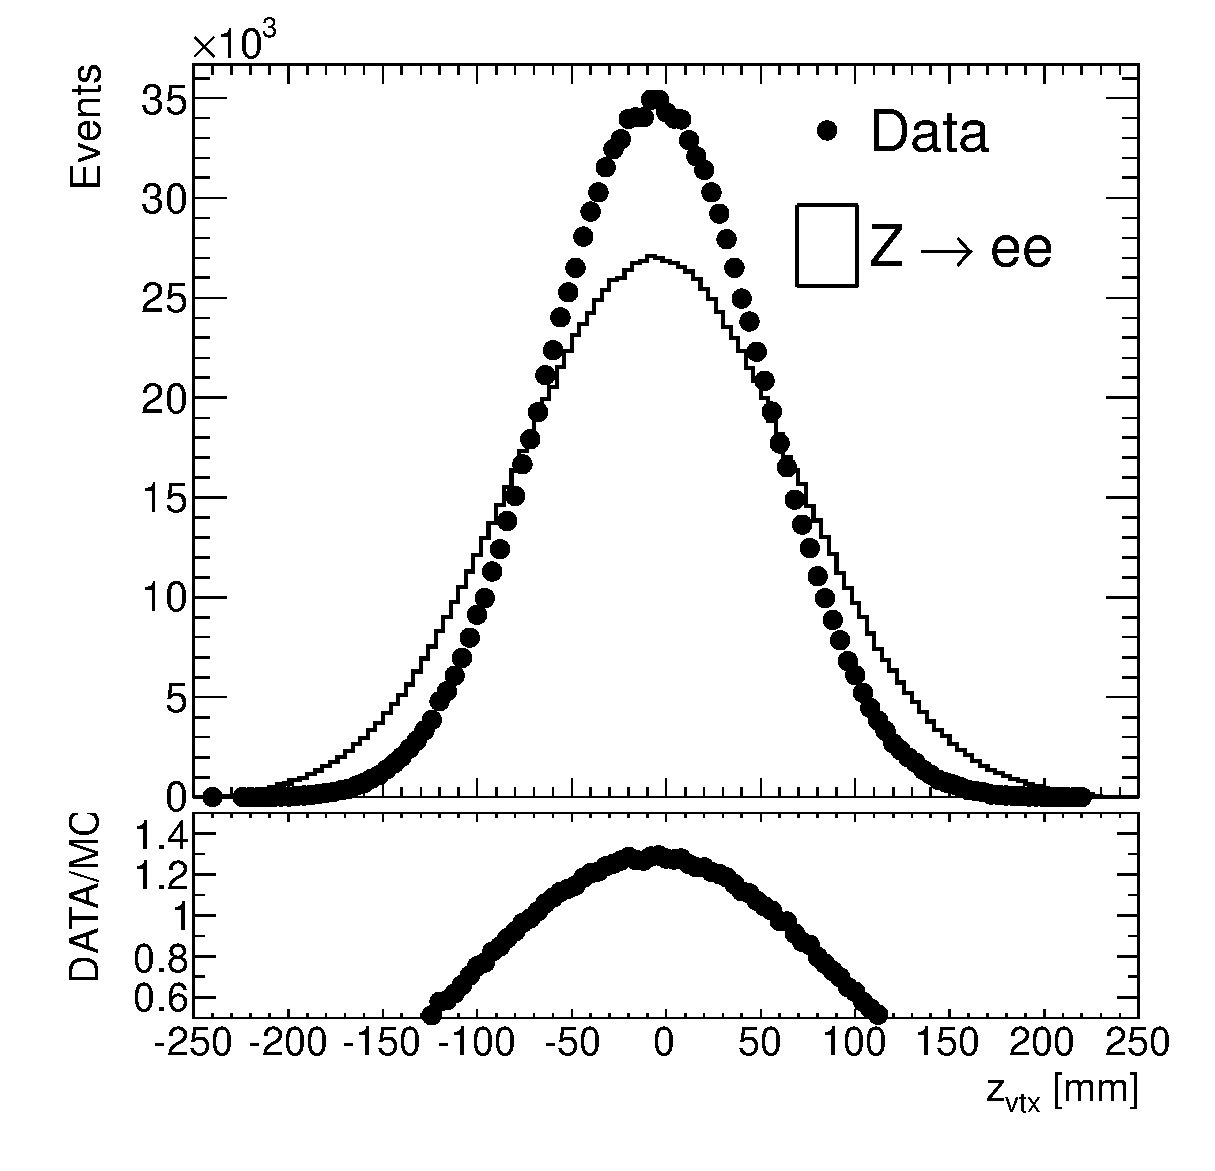
\includegraphics[width=0.32\textwidth]{figures/MCrew_zvtx_before.eps}}
\subfigure[After $z_{vtx}$ reweight] {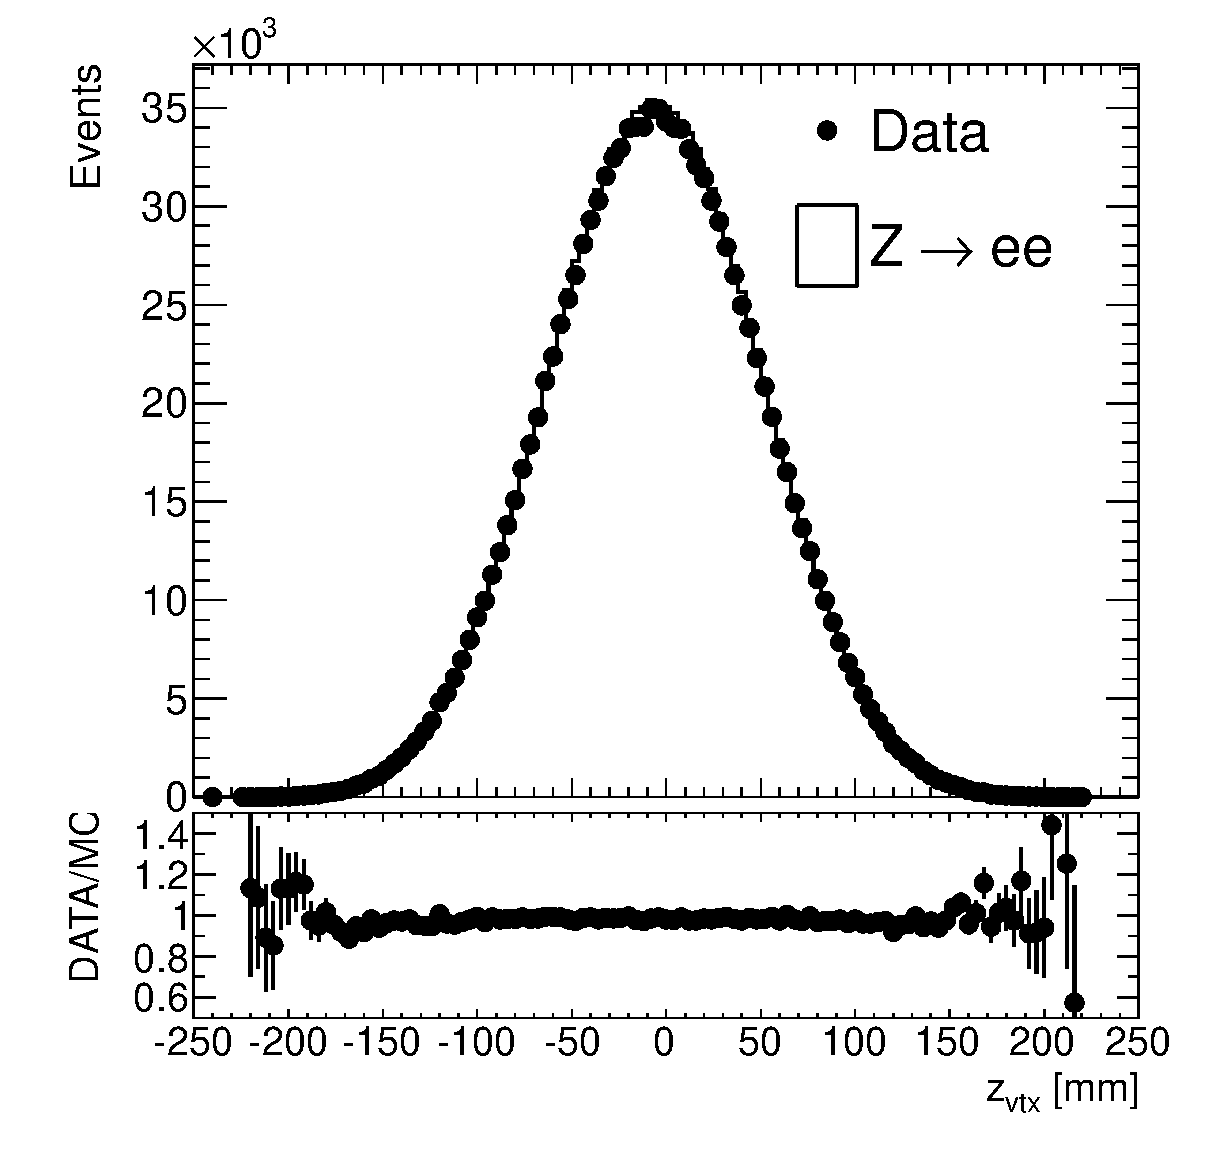
\includegraphics[width=0.32\textwidth]{figures/MCrew_zvtx_after.eps}}
\caption{The effect of the vertex spread correction applied to MC11c samples. The corrections for MC11d remained the same.}
\label{fig:MC_zvtx}}
\end{figure}

\chapter{Calibration of the EM calorimeter}
\label{sec:Calibration}

The amount of energy that the EM calorimeter registers differs very much from the total energy that the particle deposits in that calorimiter. There are several reasons for that: some energy is deposited in the presampler (i.e. outside the calorimeter), some energy is deposited away from the main cluster and is not caught by the clustering algorithms, but most importantly, there is the energy that is deposited in the so-called dead material. Both the accordion-shaped central calorimeter and the tube structured forward calorimeter have most of it's mass composed of the non-sensitive materials. Because of this design, the calorimeters must be calibrated in order to reconstruct the  true energy of the particles. Here the process of the calibration of the EM calorimeters will be described. The process consists of the $\chi^{2}$ minimization of the theoretically predicted, reconstructed energy and the truth (initial) energy of the MC sample. The MC sample is simulated using Geant4, the deposited energy is calculated based on the precise geometry model of the detector, the energy of the initial particles is then reconstructed using the theoretical model with several free parameters, and the parameters are then locked with the use of the approximation method.

\section{Theoretical overview}

The theoretically predicted formula for reconstruction of the energy is as follows

\begin{equation}
\label{eq:calib_theory}
\begin{gathered}
E_{e/\gamma} = \underbrace{a(E^{acc}_{tot}, |\eta|) + b (E^{acc}_{tot}, |\eta|) \cdot E^{clLAr}_{ps} + c (E^{acc}_{tot}, |\eta|) \cdot (E^{clLAr}_{ps})^{2}}_\text{energy in front} \\
+ \underbrace{\frac{s^{Acc}_{cl}(X,\eta)}{f_{out}(X,|\eta|)} \cdot \left( \sum\limits_{i=1,3} E^{clLAr}_{i} \right)}_\text{energy in accordion}
 \cdot \underbrace{(1+f_{leak}(X,|\eta|)) \vphantom{\left( \sum\limits_{i=1,3} E^{clLAr}_{i} \right)}}_\text{longitudal leakage}
 \cdot F(|\eta|,\varphi) \,,
\end{gathered}
\end{equation}
where

\begin{itemize}
\item $a(E^{acc}_{tot}, |\eta|)$, $b (E^{acc}_{tot}, |\eta|)$ and $c (E^{acc}_{tot}, |\eta|)$ are the parameters that are used to correct the reconstructed energy based on the total energy deposited in the accordion structure ($E^{acc}_{tot}$) and $\eta$. The first two parameters are commonly called offset and slope. The third parameter was assumed to be negligible ($c=0$).
\item $X$ is the longitudinal barycenter of the EM shower, thus representing shower depth. It is calculated as
\begin{equation}
\label{eq:calib_barycenter}
X = \frac{\sum\limits^{3}_{i=0}E^{clLAr}_{i} \cdot X_{i}}{\sum\limits^{3}_{i=0}E^{clLAr}_{i}} \,,
\end{equation}
where $E^{clLAr}_{i}$ is the amount of energy deposited in the vsrious compartments of the calorimeter: presampler in case $i=0$ and strip, middle and back for the subsequent $i$ values respectively, and $X_{i}$ is the depth, expressed in radiation length, of the longitudinal center of each compartment computed from the center of the ATLAS detector. The parameters $E^{clLAr}_{i}$ are also used in eq.~\ref{eq:calib_theory} directly.
\item $E^{clLAr}_{ps}$ is the part of the cluster energy measured in the presampler and corrected for the energy deposited in the passive materials.
\item $s^{Acc}_{cl}(X,\eta)$ is a correction factor to the Accordion sampling fraction in the cluster.
\item $f_{out}(X,|\eta|)$ is the correction for the lateral leakage of the shower, i.e. the energy deposited in the calorimeter outside the cluster.
\item $f_{leak}(X,|\eta|)$ is the correction for the longitudal leakage of the shower.
\item $F(|\eta|,\varphi)$ is the correction for the expected performance of the ATLAS detector, as described in~\cite{lib:ATLAS_perf}.
\end{itemize}

As there is no presampler in the region of the outer wheel of the EMEC, as well as the forward region of the detector (can be effectively summarized as $|\eta|>1.8$), the $E^{clLAr}_{ps}$ parameter is parameterized there as the function of the barycenter (see eq.~\ref{eq:calib_barycenter}) and the fractions of the energy deposited in every compartment of the calorimeter.

The coefficients of this equation were optimized with several MC samples with different fixed energies ranged from 5 GeV to 1 TeV.

The reconstruction of the converted and unconverted photons is done using the same technique as for the electrons, with the coefficients approximation being done separately.

\section{Calibration procedures}

\begin{figure}
\center{
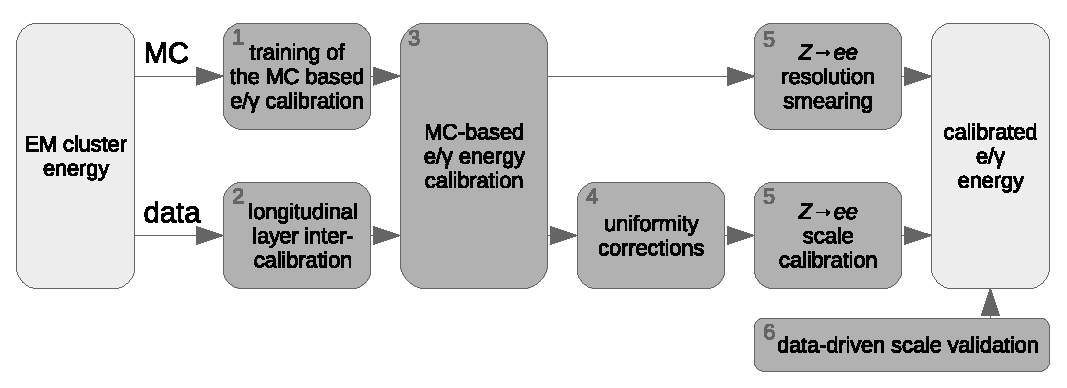
\includegraphics[width=1.0\textwidth]{figures/CALIB_main.eps}
\caption{Schematic overview of the stages of the calibration procedures for the electrons and photons in ATLAS.}
\label{fig:calib}}
\end{figure}

In order to reconstruct the energy of the EM-particles, several procedures are conducted, the overview of which can be seen in Figure~\ref{fig:calib}. The steps are as follows:

\begin{enumerate}
\item The EM cluster properties, including its longitudinal development, and additional information from the ATLAS inner tracking system, are calibrated to the original electron and photon energy in simulated MC samples. The calibration constants are determined using a multivariate algorithm (MVA), with its optimization being performed separately for electrons and converted and unconverted photons. For this calibration to work properly, the geometry of the detector must be described as precise as possible, so that the interactions of the particles with the detector material were accurate. The material distribution is measured in data using the ratio of the energy in the first-layer to the energy in the second-layer in the longitudinally segmented EM calorimeter. Measuring this ratio in data with different samples (electrons and unconverted photons) allows for a precise determination of the amount of material in front of the calorimeter and provides some sensitivity to its radial distribution.
\item Since the EM calorimeter is longitudinally segmented, the step is taken to equalize the scales of the different longitudinal layers in data with respect to simulation, prior to the determination of the overall energy scale, in order to ensure the correct extrapolation of the response in the full \pt\ range used in the various analyses.
\item The $e/\gamma$ response calibration based on MC simulation is applied to the cluster energies recorded both from collision data and MC samples.
\item A set of corrections are implemented to account for response variations not included in the simulation in specific detector regions, e.g. non-optimal high-voltage regions, geometric effects such as the intermodule widening or biases associated with the LAr calorimeter electronic calibration.
\item The overall electron response in data is calibrated so that it agrees with the expectation from simulation, using a large sample of \Zee\ events. Per-electron scale factors are extracted and applied to electron and photon candidates in data. The studies of the \Zee\ samples showed that the resolution in data is slightly worse than
that in simulation, and appropriate corrections are derived and applied to simulation to match the data.
\item The calibrated electron energy scale is validated with electron candidates from $J/\psi \to ee$ events in data. The resulting scale is dependent on $\eta$ and \pt. The scale factors extracted from \Zee\ events are assumed to be valid also for photons, with the photon-specific systematic uncertainties, which is validated with photon candidates from $Z \to ll\gamma$ events from the collision data.
\end{enumerate}

The detailed description of the calibration process can be found in~\cite{lib:calib}.

\section{Fast simulation impact}

Since both the MC11c and MC11d samples used in this analysis incorporate the results of the frozen showers fast simulation, the studies of the scaling of the calibration results were conducted. The measurements were done on the central-forward \Zee\ events in the peak mass window. The results of the comparison between samples with enabled and disabled frozen showers fast simulation system showed a difference in $\sim 1$\%~\cite{lib:calib_support}, which was then stored as a calibration correction for future use in the analysis.

\chapter{Event Reconstruction}
\label{sec:Reconstruction}

The reconstruction is the last stage of the data preparation and is the same for both genuine detector data and MC samples. The reconstruction process aims to interpret the output of the detector and to guess which particle could cause such response. Different analyses requires different focus on different types of particles, and because of that there are many reconstruction algorithms which make emphasis on different aspects of particles behavior. There are also several groups in ATLAS each of them is working on the algorithms for certain group of particles. For \Zee\ analysis the electrons are used, and the group studying the details of the electron and photon reconstruction is called "e/gamma". The group suggested several algorithms for the reconstruction of the both electrons and photons. The photons are not very important for \Zee\ analysis (although the study of the photons can improve the background estimation for the \Zee\ process, for this analysis it was not done), whereas the algorithms for electrons will be highlighted in this chapter. In section~\ref{sec:Rec_elec} the reconstruction algorithms itself will be described, while in sections~\ref{sec:Rec_elecID} and~\ref{sec:Rec_eleciso} there will be descriptions of methods to increase the quality of the reconstruction.

\section{Electron reconstruction}
\label{sec:Rec_elec}

There are several algorithms that are used to reconstruct the EM-particles (electrons and photons), each of them reconstructs its own set of particles for every event. To distinguish which particle was reconstructed by what algorithm, the "author" field was introduced. The field consists of 5 bits each of them can be 1 or 0 depending on whether the corresponding algorithm reconstructed that particular particle (one particle can be reconstructed by more than one algorithm). The field is then interpreted as decimal integer. The list of algorithms is as follows:
\begin{itemize}
\item {\bfseries AuthorElectron} Electron reconstructed by standard cluster-based algorithm. It requires both EM cluster and a matching track.
\item {\bfseries AuthorSofte} Electron reconstructed by the track-based algorithm. This algorithm doesn't require EM cluster, only the track. This author can overlap with the previous.
\item {\bfseries AuthorPhoton} Photon reconstructed by standard cluster-based algorithm. Same as the first, only for photons.
\item {\bfseries AuthorFrwd} Electron reconstructed by the Forward cluster-based algorithm. As the inner detector doesn't provide tracks for $\eta > 2.5$, the algorithm for forward particles uses only the cluster, and is tuned to be used in the forward detectors.
\item {\bfseries AuthorRConv} Photon that is duplicated with electron. Is used to mark the special cases when both electron and photon reconstruction algorithms return positive for the same particle.
\item {\bfseries AuthorTrigElectron} and {\bfseries AuthorTrigPhoton} Mark the trigger particles. The triggers were discussed in Sec.~\ref{sec:ATLAS_trigger}.
\end{itemize}

Because of the much difference between the algorithms for central and forward electrons, the reconstruction process for both will be discussed separately.

\subsection{Central}

The central electron is the electron with $\eta < 2.5$. In this area of the detector both EM calorimeter and tracker are present, so the reconstruction algorithms can make use of both. In the central region there are two  EM calorimeters: EMB and the outer ring of the EMEC, and the standard cluster-based algorithm behave slightly different in them. In current analysis only the central electrons reconstructed by the standard algorithm were used, so only it will be described. It consists of three main stages~\cite{lib:elec_reco}: the initial search for a EM-cluster, the track matching and the final reconstruction of the electron candidate. For the initial search the sliding-window algorithm is used with the size of $3 \times 5$ cells in units of $0.025 \eta \times 0.025 \varphi$ each. The seeding energy threshold for the algorithm is 2.5 GeV, and from the MC calculation of W and Z decays, the efficiency is expected to be about 97\% at $E_{t} = 7$ GeV and almost 100\% at $E_{t} > 20$ GeV. During the second stage every cluster is matched with a track reconstructed from the tracker. The reconstruction of the track is pretty straightforward: it is seeded by the hit in the innermost layer of the tracker, and then propagated outside by connecting the closest hit of the adjacent layer~\cite{lib:track_reco}. The matching algorithm tries to find the track with the impact point within of $|\Delta\eta| < 0.05$ and $|\Delta\varphi| < 0.1$. The size of $\Delta\varphi$ is taken bigger to account for the possible bremsstrahlung losses during the pass of the solenoidal magnetic field. If there are several such tracks, the closest one is chosen, with the priority given to the tracks with the hits in pixel detector or SCT (as opposed to the TRT, see section~\ref{sec:ATLAS_tracker}). If no track can be found, the candidate is classified as a photon, and the photon-reconstruction algorithm is used for it. The final stage is the calculation of the cluster energy and other cluster variables. It is during this stage, when the differences between EMB and EMEC come into play. The size of the window differs for these two detectors: it is $3 \times 7$ cells in EMB and $5 \times 5$ in EMEC in the same units of $0.025 \eta \times 0.025 \varphi$. The $\eta$ and $\varphi$ spatial coordinates of the electron are taken from the matched track at the interaction vertex, the energy is calculated from the cluster. Still, all the variables from both cluster and matched track are saved and available separately for the needs of the analysis.

\subsection{Forward}

The forward region of the calorimeter starts from $\eta = 2.5$ and includes two detectors: the inner wheel of the EMEC and FCAL. There is no tracker in this region, so the reconstruction algorithm deals only with clusters. Because of this the reconstruction algorithm can't make a difference between electrons and photons, and electrons and positrons. For this region another cluster-construction algorithm is used which is called "topological clustering"~\cite{lib:elec_reco_fwd}. This algorithm is very effective at noise suppression, which is very important for forward region. The algorithm is seeded by a single cell with an energy significance which is above a high signal to noise ratio threshold. Then the cluster is expanded by adding the neighbor cells with the said ratio being above the medium threshold, and then finalized by taking in all the cells above low threshold. The standard configuration for this algorithm for EM calorimeters is called "EM~633", with the thresholds being 6, 3 and 3 respectively. If the process of cluster expanding proceeds to the hadron calorimeter, the configuration "Had~420" is used. The spatial coordinates of the reconstructed electron is then calculated as a barycenter of the cluster. This algorithm produces the variable-sized cluster, as opposed to the sliding-window algorithm, which produces a cluster with a fixed size. Because of the three-dimensional nature of the cluster expanding used in the algorithm, it is very effective in suppressing the pileup. The effectiveness in terms of electron reconstruction is predicted (via MC simulation) to be above 99\% for the electrons with $E_{t} > 20$ GeV. To be reconstructed, the electron candidate must have $E_{t} > 5$ GeV, and have no significant energy deposits in the hadron calorimeter.

\section{Electron identification}
\label{sec:Rec_elecID}

The electron identification is the next step of the data preparation, and is aimed to reduce the number of false-positive cases of the reconstruction algorithms such as background hadrons from semileptonic decays or photon conversions. The identification is implemented using several cuts on cluster, track, and combined cluster-track variables. For use in the analysis, three sets of cuts were introduced, with every consecutive being a superset of the predecessor. These sets are named loose, medium and tight. Each one of them is more effective in background suppression than the previous, but is less effective in terms of identification efficiency, which is they increase the amount of false-negative cases.

The description of these identification criteria is described below.
\begin{itemize}
\item {\bfseries Loose}: This is the least demanding criteria, that performs only a basic cuts on the reconstructed electron candidate. It takes into account the shower shape variables from the EM calorimeters and the hadronic leakage information. The most important shape variables can be seen in Fig.~\ref{fig:REC_shower_shapes}, and they usually show the fracture of the energy deposited in some parts of the cluster (in the beginning, and the end, in the center etc), relative to the whole energy of the cluster. The distributions usually have peaks, where the "good" electrons are located, and tails, with "bad" electrons. The thresholds for each variable is picked experimentally. The criteria also increases the requirements on the quality of the track and of the track-cluster matching. It improves the rejection of the hadronic background by a factor of $\sim 5$ in the range $30 < E_{t} < 40$ compared to the bare reconstruction algorithms, while not affecting the identification efficiency.
\item {\bfseries Medium}: This is an overall a more demanding version of the "loose" criteria, with a more demanding requirements on the same variables. It also introduces several new requirements, mostly on the track, the most important one being the requirement of the hit in the innermost layer of the tracker, which aims to suppress the photon conversion background. It is $\sim 10$ times more efficient in background rejection than "loose", but has a drawback of having a worse identification efficiency.
\item {\bfseries Tight}: This one makes a full use of all the identification tools available. In addition of more strict requirements for every variable used in "medium", it also makes new: on the track extension in the TRT and on the ratio between track momentum and cluster energy. It also takes into account the list of reconstructed photon conversions associated with the same vertex. Overall, it increases the the background rejection by the factor of two with respect to "medium".
\item {\bfseries Forward Id}: For the forward region of the calorimeter, the identification criteria follow the similar pattern as for the central region, because of lack of the tracking information, only the shower parameters are taken into account. The shower shape, the longitudal, transverse and normalized lateral momenta are all used for the identification process. In 2011, the pileup increased drastically for the forward region, so the criteria became more strict, and are derived from the previous data. The thresholds come in four bins based on the number of primary vertexes reconstructed in the event ($N_{PV} = 1-3$, $4-6$, $7-10$, $>10$). All the three criteria use the same set of variables, but progressively increase the thresholds, with the {\itshape fwdTight} rejection factor being 2 to 3 times bigger than the {\itshape fwdLoose} one.
\end{itemize}

The criteria for the forward electrons are different, since the forward region lacks the tracker, and has a significantly higher pileup. The cuts are applied to the cluster itself, and take into account such parameters as longitudinal second momentum, transverse second momentum, normalized lateral momentum and so on. The fact that the reconstruction algorithm for forward region produces a three-dimensionally shaped cluster helps greatly. The loose, medium and tight criteria are also defined for the forward region, but work on the same variables, only with consecutively stricter requirements.

For 2011 the new set was introduced which was attuned more attuned to the data and was more effective at background-suppression. The new set was called "IsEM++" criteria (the previous was called just "IsEM"), and consist respectively of loose++, medium++ and tight++. The difference between the sets is mostly the tunes to the variables thresholds.

\begin{figure}
\center{
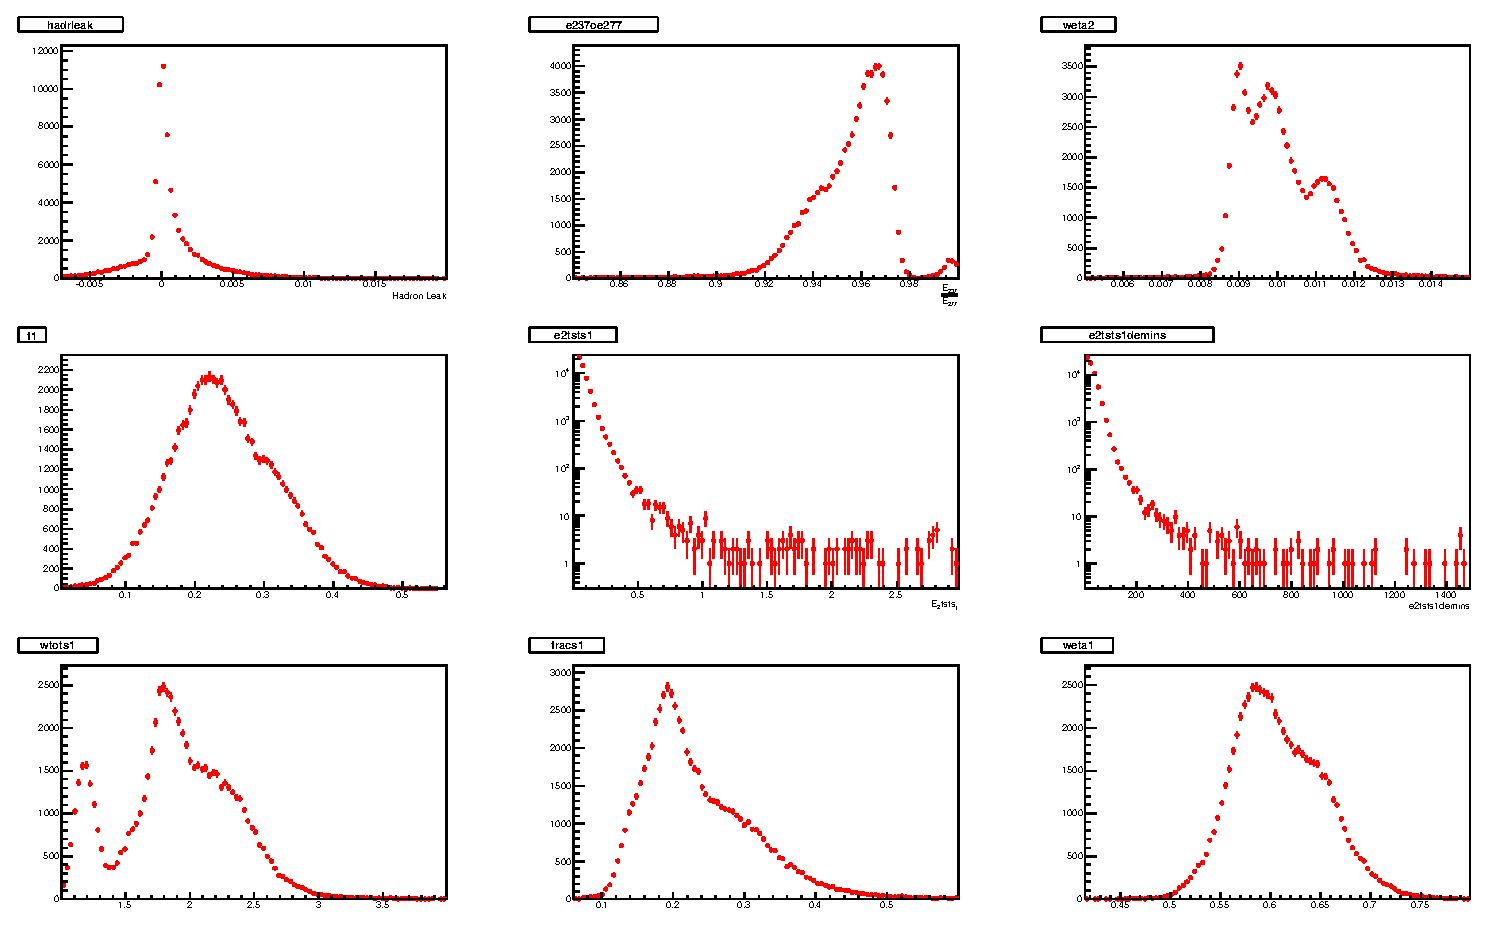
\includegraphics[width=1.0\textwidth]{figures/REC_shower_shapes.eps}
\caption{Some of the shower shapes variables shown for MC-simulated electrons. All of these variables are used for the electron identification in the central region.\tbu A BETTER PLOT}
\label{fig:REC_shower_shapes}}
\end{figure}

\section{Electron isolation}
\label{sec:Rec_eleciso}

To further suppress fake electron background, the isolation check is also used. The isolation check relies on Etcone variable, which is the sum of the energy in a cylinder surrounding the cluster, excluding the cluster itself. Although we use the cylinder, in a sense that it is a round shape with a constant $\Delta R$ where $\Delta R = \sqrt{\Delta\eta^{2} + \Delta\varphi^{2}}$, in real geometry it looks like a cone, that's why all the names of the isolation variables contain "cone".  The radius of the cylinder that was used is written in the name of the variable, so there are several of them, e.g. Etcone20, Etcone40, etc, where 20 or 40 means $\Delta R = 0.20 , 0.40$~\cite{lib:reco_iso}. The Etcone variable can use cluster $E_{t}$ as well as track $E_{t}$, and different isolation criteria use one or another or both. The said criteria is just the cut on the ratio of the Etcone energy to the cluster energy. If the ratio is low, we are dealing with the high-isolation electron. This is the best-case scenario. The higher values of the ratio means low-isolation electron, the high error in energy reconstruction is expected for this kind of electrons. The high value of the ratio means that the electron is most likely a fake: a misidentified muon or hadron jet with a mismatched track.

For \Zee\ central-forward analysis, the isolation cuts named Iso98 for Etcone20 and Iso97 for Ptcone40 were used for the central electron. It allowed to reduce the background to the factor of 2, while still retaining the electron efficiency of 97-98\%.

\chapter{Analysis Software (ZeeD)}
\label{sec:ZeeD}
ZeeD (\Zee\ DESY) is a softvare solution, developed internally by the DESY ATLAS standard model group under the supervision of Dr. A. Glazov. It is based on the \Athena\ framework that is largely used in ATLAS, but uses it mostly for the input data reading, which is in the AOD format which is also standard for ATLAS. For performance reasons, the first step in the analysis is the conversion of the data in the ZeeD internal format called TTrees (which is actually the name of the class in the ROOT framework which is used in this format, but in this work any mention of TTrees means this data format). This conversion allows the substantial speedup of the analysis, as well as considerably reduce the space needed for the data storage. The later stages of the analysis include the selection (application of cuts), reweighting (in case of MC) and plotting. ZeeD also allows to apply the systematic shifts as well as use ToyMC for uncertainties propagation studies. All these stages and subsystems of ZeeD will be described in this section.

\section{TTrees}
\label{sec:ZeeD_TTrees}

The data from the ATLAS detector comes in the form of the AOD files, which a special format based on the ROOT data file format and developed internally by the ATLAS. The format allows the seamless reading and writing of the various data objects (e.g. tracks, EM clusters, reconstructed particles, etc) within the \Athena\ framework. In AOD files all the information reconstructed from the collision is stored. In case of simulated events (i.e. MC) there is also the information about the generated particles, the so-called "truth particles", which can be used to determine the efficiency of the reconstruction algorithms and the analysis software.

Most of the information stored in the AODs is unneeded for the \Zee\ analysis, which only needs reconstructed electrons. And not even all the information available for the electrons is needed, as we only need enough to apply cuts and construct various differential cross-sections. During the analysis workflow, ZeeD uses about $0.1\%$ of all the information stored in the AODs, but because of the framework structure, all the content of it should be read from the store and preloaded into the memory, which consumed most of the time needed for the analysis iteration. Also, because of the nature of the ATLAS data storages and the GRID farms used for the analysis, it was prone to errors, and it would require several attempts and consume much time to finish even one iteration.

The solution for this problem is to extract the needed information from the AOD files and store it in the simplified structure in ROOT ntuples. Similar solution was later used for the AOD successor - xAOD format. But whereas xAOD allows all this to be done automatically, for the 2011 the custom tool for manual conversion had to be developed. The software chain for the TTree writing is no different from the analysis chain. The data is read from the AODs, the preselection cuts are applied to reduce the amount of data, and the output information is written out, which in this case is the raw events.

Because of this similarity, the same software - ZeeD - was used for the TTrees production as well. It is capable of reading the data from AODs, it has all the cuts applicable for preselection, and it is capable of outputting any kind of data from the selected events. With the corresponding setup, the ZeeD workflow will be suitable for this production.

\section{Boson Finder}

The main target of all the analyses that are conducted using the ZeeD software are the Z bosons, so finding all the possible Z boson candidates in every event is always the first task. The ZeeD component that does that job is the boson finder class. On the basic level it just creates a boson candidate for every possible pair of electrons, but further in the analysys it keeps track of all the bosons and records all the intermediate results for each one. Ultimately, we won't accept more than one boson from any event, so every boson candidate is assigned a special "score" of how well it passes the various cuts. When there are several boson candidates that pass all the required cuts, the candidate with the highest score is picked for the final results. In case of the final \Zee\ analysis this situation is impossible, though, a we require not more than two suitable electrons. This mechanism is used for various tests and cross-checks.

\section{Cuts}

The analysis implications of different cuts will be discussed in the Sec.~\ref{sec:Sel_cuts}. Here we'll discuss the technical aspects of the event selection.

From the technical point of view, every cut is a restriction on one or several variables of the reconstructed event. Every event can pass or fail every cut, and the infrastructure should be able not only to provide information whether some event passed all the cuts or not (which is the only thing that is important for the analysis itself), but also to show the results of all the cuts separately. This is called a "cut-flow" and it is used for debugging purposes and cross-checking. In the situation when different groups using different software come to different results for the same ananlysis, the ability to find out on which cut every particular event was filtered out is very helpful. With it we can find out which cut gives different results across different analysis groups.

The other functionality which is needed from the cuts facility is the cut reversal which is used for the background estimation. The background estimation methods (discussed later in Sec.~\ref{sec:Bkg}) requires to select the events where electron pass some specific cuts, but fail some other specific cuts. To achieve that, the cuts framework construct the bit-mask for every event, where every bit corrseponds to some cut, and displays whether that event passed or failed that cut. After the bit mask is composed, we can compare it to the desired bit-mask, and include or exclude the event from the analysis.

\section{Reweighting}

The reweighting of the MC events is used for the fine-tune of the simulation with relation to the real data. The weights are calculated based on the well defined distributions of the data (such as the trigger efficiencies) and are to bring the corresponding MC distributions in accordance with the data. The calculation of the weights is done using some well-measured process. For instance, \Zee\ decay is good for calculating the trigger efficiency, since it has a low background in the peak region, and has two electrons which allow the use of the tag and probe method. The calculation of the weights is thus done by conducting the same analysis on MC and real data without any corrections whatsoever, and then comparing the distributions, for which we want to introduce reweighting. Weights are usually applied in bins, so the result of the weight calculation would be a histogram, sometimes two-dimensional, which would cover the kinematic plane for the variable being reweighted. Apart from the weight itself, the statistical and systematical uncertainties for every bin are also calculated, and stored in the similar histograms.

After the weights are calculated, they are used during the analysis. The weights are picked for every event based on its properties, and then the final weight of the event is calculated by multiplying all the weights from different corrections. This weight is later used during the histograms plotting. Since every weight comes with the statistical and systematical uncertainties, they also contribute to the calculation of the final error for the analysis. The process of calculation of the impact of different uncertainties to the final combined error would be discussed in the sec.~\ref{sec:ZeeD_toymc}.

\section{Histogram managers}

The results of the analysis are the histograms, showing the various distributions of the physical quantities. The facilities responcible for that are the histogram managers. Each manager represents some aspect of the analysis, and creates and fills one or several histograms, which are thus grouped by their role in it. Each of the managers can be attached or detached during the launch setup, which allows to conduct various analyses with the same software, as long as this analysis deals with electrons, muons, and missing $E_{t}$ (the only kind of data that ZeeD extracts from the egamma data stream).

For the \Zee\ analysis the important managers would be an electron manager (plots the various distributions of the electrons properties, such as energy, $E_{t}$, geometrical variables, etc), a ZCF manager (plots the properties of the central-forward Z-bosons), and (in case of MC) the truth managers (plots the truth information for the given event).

There is also one special histogram manager, which actually doesn't plot any histograms, but uses the same interfaces. It is the ZeeD TTree writer, which dumps out the content of the event in the ROOT tuples. This histogram manager is used to produce the TTrees that were previously discussed in sec.~\ref{sec:ZeeD_TTrees}.

\section{Systematics and ToyMC}
\label{sec:ZeeD_toymc}

One of the most important aspects of the analysis is the error estimation. The calculation of the statistical error can be done analytically, since it is subjected to the law of the large numbers. Estimation of the systematical errors can't be done that way, because the propagation of the error through the analysis procedures is complex, and can't be described analytically. Same applies to the error propagation from the underlying parameters, such as efficiencies and corrections.

To propagate the errors, there was introduced the system of systematic shifts. The quantity, the effect of error of which is to be measured, is shifted up or down to the amount of it's combined error, and the resulting shift in the final distributions is measured as a contribution of this quantity's error to the final combined error. This system is easy, but it's inefficient in the situations of the relatively large statistical errors, because it treats them as systematical.

To properly propagate the statistical error, the system of ToyMC was introduced. The ToyMC system conducts many (usually several hundreds) of analyses, with the respectable quantities shifted within its combined error according to the Gauss distribution. In the output, we are getting the similar distribution of the final values, which can be used to properly estimate the final combined error. The evolution of the ToyMC method was the Combined ToyMC, which could be used to propagate both systematical and statistical errors simultaneously, thus instantly getting the combined error as an output.

\chapter{Event Selection}
\label{sec:Selection}

The event selection is one of the main phases of the analysis, which is focused on suppressing of as much as possible background events while keeping the signal events. The process of selecting the suitable events goes in three stages. The first stage is the online triggers, which, as name suggests, occurs during the data taking, even before the data is written on the storage. The specifies of the trigger work was described in the corresponding section (see Section~\ref{sec:ATLAS_trigger}). The other two stages are the pre-selection and analysis selection (or just selection), and they are specific to our analysis software ZeeD (described later in Section~\ref{sec:ZeeD}), although the division of the selection in such a way is a common practice because of the large amount of data. These two stages would be described in the following sections.

\section{Analysis preselection}
\label{sec:Sel_pre-sel}

The goal of the preselection stage is to reduce the amount of data (by removing "non-interesting" events) while not biasing the samples in regards of the \Zee\ analysis. There are two flavors of preselection: the two-electron preselection and the one-electron. The cut for the two-electron stream requires $\pt > 14$ GeV for both electrons and the cut is $\pt > 20$ GeV for one-electron. For the central-forward \Zee\ analysis the single-electron stream is mostly used, but the di-electron is also used in some cases, for instance for the trigger efficiency scale factors calculation (tag\&probe method). Such cuts do not affect any possible distribution within the \Zee\ analysis, be it the signal or the background studies. During the preselection stage we also extract all the data that is relevant to the analysis, while disregarding all the rest of the data stream (e.g. muons, jets and so on). This allows us to reduce the physical amount of data from terabytes to just mere gigabytes, and to speed-up the analysis by the factor of hundreds. The resulting pre-selected data is very similar to the D3PD from the programming point of view (which is a commonly used data format that was developed after AOD, and was later incorporated in AOD successor - xAOD), but is designed specifically for the needs of \Zee\ analysis (see Section~\ref{sec:ZeeD_TTrees} for details).

\section{Analysis cuts}
\label{sec:Sel_cuts}

The application of cuts is one of the most important parts of the analysis. During this stage we try to suppress the background while keeping the signal intact. The cuts can be divided in three categories: the technical cuts, the kinematic cuts and the electron "goodness" cuts. The technical cuts are applied on a per-event basis. Here we check that no problems were encountered during the event taking. This includes a so-called good run list, which excludes the events taken during the runs with observed problems in the detector, and the OQ-map (object quality map) which is a list of a regions of the calorimeter which are known to be faulty, and so the cut excludes all the events with at least one electron depositing energy in one of those regions.

The kinematic cuts deal with the kinematic properties of the electrons: we require only two electrons, with one being inside the central region and one inside the forward region, both are reconstructed with the proper reconstruction algorithm and both meeting the selection requirements for the kinematic properties.

Finally there are cuts on the quality of the electrons, which involve passing certain IsEM criteria and a certain isolation criteria.

Every group of cuts will be described in details.

\subsection{Data quality cuts}
\label{sec:Sel_GRL_OQ}

\begin{itemize}
\item {\bfseries Good Run List}: This cut drops every event that was taken during the non-successful runs of the LHC. The list of the good runs is compiled by the Data Quality group and is the same for all analyses.
\item {\bfseries Object Quality Maps}: This cut drops every electron that was reconstructed inside one of the faulty regions of the calorimeter. The events with such electrons can still be used in the analysis, if they have another two good electrons.
\item {\bfseries LAr Veto}: This cut drops every event that was taken while the LAr calorimeter was malfunctioning, as indicated by the \texttt{LArErrorState} property.
\end{itemize}

\subsection{Kinematic cuts}
\label{sec:Sel_kinematic}

\begin{itemize}
\item {\bfseries Two good electrons per event}: This cut drops all events that have the number of good electrons other than two. The Drell-Yan process produces exactly two electrons, so everything else is a background for our analysis. In case of central-forward analysis, the cut can be renamed as {\bfseries 1+1 good electrons per event}, as we require exactly one good electron in the central region, and one in the forward region.
\item {\bfseries Minimum electron \pt}: This cut drops all electrons with the $\pt < 20$~GeV. We do not have adequate efficiency corrections for the electrons with low \pt.
\item {\bfseries Electron $|\eta|$}: This cut drops all electrons which have a cluster that is reconstructed outside the required $\eta$ regions: $|\eta| < 2.47$ for the central electron and $|\eta| > 2.52$ for the forward electron.
\item {\bfseries Electrons are outside the crack regions}: This cut drops all electrons reconstructed inside the crack regions of the calorimeters. For the central electrons the cracks are $1.47 < |\eta| < 1.52$ and $|\eta| > 2.47$, for the forward electrons it is $3.16 < |\eta| < 3.35$
\item {\bfseries Z boson mass}: This cut drops all events with the di-electron mass outside the mass window range ($66 < |M_{ee}| < 116$~GeV for peak mass and $116 < |M_{ee}| < 150$~GeV for high mass regions).
\item {\bfseries Number of tracks at primary vertex}: This cut drops all events that do not have a vertex with at least three tracks.
\end{itemize}

\subsection{Electron quality cuts}
\label{sec:Sel_isem_iso}

\begin{itemize}
\item {\bfseries A track for the central electron}: This cut drops all events with the central electron having no track. The "author" cut which requires the specific author for every electron supersedes this cut, but it is kept for compatibility purposes.
\item {\bfseries Central electron IsEM}: This cut requires the central electron to satisfy the IsEM criteria (described in Section~\ref{sec:Rec_elecID}).
\item {\bfseries Forward electron IsEM}: This cut requires the forward electron to satisfy the IsEM criteria.
\item {\bfseries Central electron isolation}: This cut requires the central electron to satisfy the isolation criteria (described in Section~\ref{sec:Rec_eleciso}).
\item {\bfseries Electron author}: This cut requires the proper author (described in Section~\ref{sec:Rec_elec}) for both central and forward electron.
\end{itemize}

The cutflows, i.e. the tables that shows how many events pass any given cut, can be seen in Tab.~\ref{tab:sel_cutflow_data} for data and in Tab.~\ref{tab:sel_cutflow_MC} for the signal MC sample. The relative efficiency shows how many events pass the cut relative to the previous cut, while the absolute efficiency shows the number of events relative to the total number of events.

\begin{table}
\centering
\begin{tabular}{@{}lrrr@{}} \hline \hline
 Cut & events & $\epsilon_{rel}$ [\%] & $\epsilon_{abs}$ [\%] \\\hline
 All events (after pre-selection)  &    234255443 & &   100.00000 \\
 primary vertex w. $>2$ tracks &    234127638 &     99.9454 &    99.94544 \\
 veto LAr noise bursts & 233365291 &     99.6744 &    99.62001 \\
$|\eta_{cnt}| < 2.47$, $2.5<|\eta_{fwd}|<4.9$ &    138946695 &     59.5404 &    59.31418 \\
excl. $1.47 < |\eta| < 1.52$ &    127877309 &     92.0334 &    54.58883 \\
excl. $3.16 < |\eta| < 3.35$ &    124775277 &     97.5742 &    53.26462 \\
$pt_{e}^{cent.} > 25$\,GeV &    74478333 &     59.6900 &    31.79364 \\
$pt_{e}^{fwd.} > 20$\,GeV &      8404968 &     11.2851 &     3.58795 \\
Author &     8404244 &     99.9914 &     3.58764 \\
good object quality &     8338286 &     99.2152 &     3.55948 \\
 Tight++ &      1537446 &     18.4384 &     0.65631 \\
 FwdTight &       370376 &     24.0903 &     0.15811 \\
 Iso98Etcone20 &       355029 &     95.8564 &     0.15156 \\
 Iso97Ptcone40 &       340852 &     96.0068 &     0.14550 \\
 single-lepton trigger &       339235 &     99.5256 &     0.14481 \\
 MaxTwoGoodElectrons &       339235 &    100.0000 &     0.14481 \\\hline
 $66 < m_{ee} < 116$~GeV &       321575 &     94.7942 &     0.13728 \\
 $116 < m_{ee} < 150$~GeV &         7740 &        2.28 &     0.0033 \\ \hline \hline
\end{tabular}
\caption{The cutflow for the \Zee\ CF data selection both for peak and high mass windows.}
\label{tab:sel_cutflow_data}
\end{table}

\begin{table}
\centering
\begin{tabular}{@{}lrrr@{}} \hline \hline
 Cut & events (weighted)  & $\epsilon_{rel}$ [\%] & $\epsilon_{abs}$ [\%] \\\hline
 All events (after pre-selection) &     19783527.83 &             &   100.00000 \\
 primary vertex w. $>2$ tracks &     19659928.15 &     99.3752 &    99.37524 \\
 veto LAr noise bursts &     19659928.15 &    100.0000 &    99.37524 \\
$|\eta_{cnt}| < 2.47$, $2.5<|\eta_{fwd}|<4.9$ &     12425328.01 &     63.2013 &    62.80643 \\
excl. $1.47 < |\eta| < 1.52$ &     11837779.90 &     95.2714 &    59.83655 \\
excl. $3.16 < |\eta| < 3.35$ &     11431076.75 &     96.5644 &    57.78078 \\
$pt_{e}^{cent.} > 25$\,GeV &      7959710.26 &     69.6322 &    40.23403 \\
$pt_{e}^{fwd.} > 20$\,GeV &      3207445.87 &     40.2960 &    16.21271 \\
Author &      3206917.09 &     99.9835 &    16.21004 \\
good object quality &      3186720.53 &     99.3702 &    16.10795 \\
 Tight++ &      2228171.55 &     69.9205 &    11.26276 \\
 FwdTight &      1684155.81 &     75.5847 &     8.51292 \\
 Iso98Etcone20 &      1661813.91 &     98.6734 &     8.39999 \\
 Iso97Ptcone40 &      1629799.05 &     98.0735 &     8.23816 \\
 single-lepton trigger &      1584699.06 &     97.2328 &     8.01019 \\
 MaxTwoGoodElectrons &      1584699.06 &    100.0000 &     8.01019 \\ \hline
 $66 < m_{ee} < 116$~GeV &      1542376.88 &     97.3293 &     7.79627 \\
 $116 < m_{ee} < 150$~GeV &        42206.05 &        2.66 &     0.21 \\ \hline \hline
\end{tabular}
\caption{The cutflow for the \Zee\ CF MC selection both for peak and high mass windows. The number of events is corrected for weights.}
\label{tab:sel_cutflow_MC}
\end{table}

\chapter{\Zee\ cross section measurement}
\label{sec:ZeeCrossSec}

The measurement of the \Zee\ production cross-section is the main purpose of this work, and the details of the methodology of the measurement are discussed in this chapter.

The ATLAS detector, like every other physical device, has its limitations, and the signal obtained from the detector is thus distorted. The process of estimating the results that would have been achieved with an ideal detector based on the results using the real detector is called the unfolding process (also called "deconvolution" or "unsmearing" in mathematical literature), and is the one of the most important stages of the measurement of the cross-section. The main idea of the unfolding is that if $f_\mathrm{meas}(x)$ is the spectrum of a value measured using the real detector and $f_\mathrm{ideal}(x)$ is the the spectrum that would have been measured with an ideal detector, then
\begin{equation}
f_\mathrm{meas}(x) = \int R(x|y) \, f_\mathrm{ideal}(y)dy
\end{equation}
where $R(x|y)$ is the detector response function. In case of binned distribution this equation can be written as
\begin{equation}
v^\mathrm{meas}_i = \sum_j R_{ij} \, v^\mathrm{ideal}_j \:\:\:\:\: i,j = 1, ... ,N
\end{equation}
where $v^\mathrm{meas}_i$ and $v^\mathrm{ideal}_i$ are the measured and ideal values accordingly. Generally speaking, the number of bins in $v^\mathrm{meas}$ and $v^\mathrm{ideal}$ spectra can be different, and the matrix $R_{ij}$ would be rectangular, but in this analysis the same binning is used for both. The main task of unfolding is to determine the response matrix, and then to calculate the unfolding matrix based on it. The easiest solution would be to just invert the response matrix:
\begin{equation}
v^\mathrm{ideal}_i = \sum_j R^{-1}_{ij} \, v^\mathrm{meas}_j \:\:\:\:\: i,j = 1, ... ,N
\end{equation}
which is not always the best choice, because it produces very large distortions in case of limited statistics. The task of propagating the systematic uncertainties through the unfolding process also must be solved.

There are two methods of unfolding that are usually employed by ATLAS analysis groups: the bin-by-bin correction, and the Bayesian unfolding~\cite{lib:zcs_unfolding}. There are several advantages and disadvantages in both methods, but the main criteria of the preference of the Bayesian or bin-by-bin unfolding lies in two important factors: purity and stability. These two factors are calculated as follows:
\begin{equation}
P^{i} = \frac{N^{i}_{\text{rec\&gen}} }{ N^{i}_{\text{rec}} }\,, \; \;
S^{i} = \frac{N^{i}_{\text{rec\&gen}} }{ N^{i}_{\text{gen}} }\,,
\end{equation}
where:
\begin{itemize}
\item {\bfseries $N^i_{\text{rec\&gen}}$} is the sum of event weights which were generated and reconstructed in bin $i$.
\item {\bfseries $N^i_{\text{rec}}$} is the sum of event weights reconstructed in bin $i$.
\item {\bfseries $N^i_{\text{gen}}$} is the sum of event weights generated in bin $i$.
\end{itemize}

The purity is thus a measure of in-migration, which shows the amount of foreign events reconstructed in the given bin, while the stability is a measure of the out-migration, which shows the amount of events that were reconstructed in other bins for every given bin. In terms of response matrix, the distribution with high purity and stability will have a mostly diagonal matrix. This will warrant for a use of a bin-by-bin unfolding. This method, dealing with every bin independently, will produce a diagonal matrix. But if the migrations between bins are substantial, ignoring it will highly increase the distortions in the unfolded results, in which case the Bayesian unfolding becomes preferable. The results of the purity and stability studies for the \Zee\ central-forward analysis suggested that the Bayesian unfolding would be more effective (see Figure~\ref{fig:ZeeCS_purity_stability} for the exact values of the purity and stability of the 2011 \Zee\ central-forward analyses). In the following sections the methodology for both bin-by-bin and Bayesian unfoldings are shown. Also, the methodology of the result combination is explained, which mathematically is very close to unfolding, as it is the same inverse problem.

\begin{figure}
  \centering
  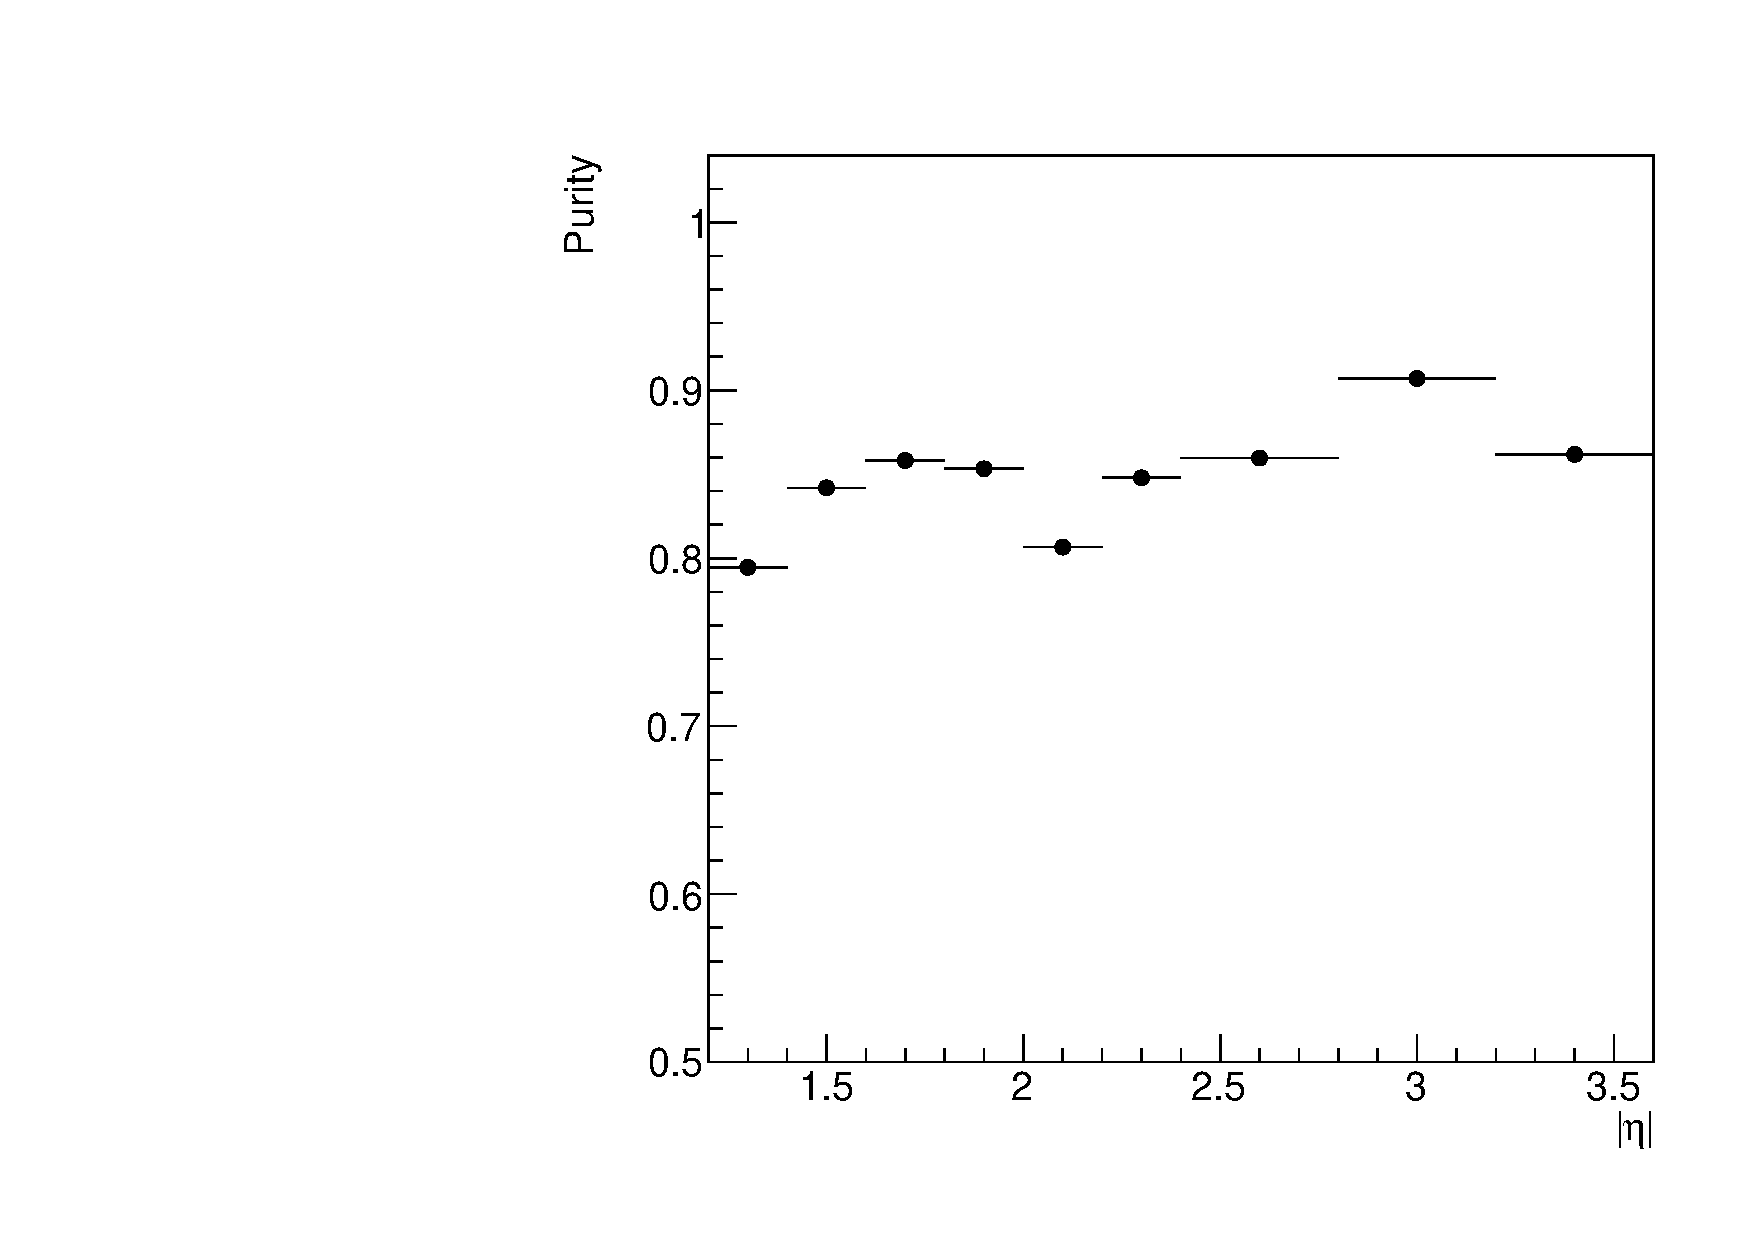
\includegraphics[width=0.45\textwidth]{figures/ZCF_purity_peak}
  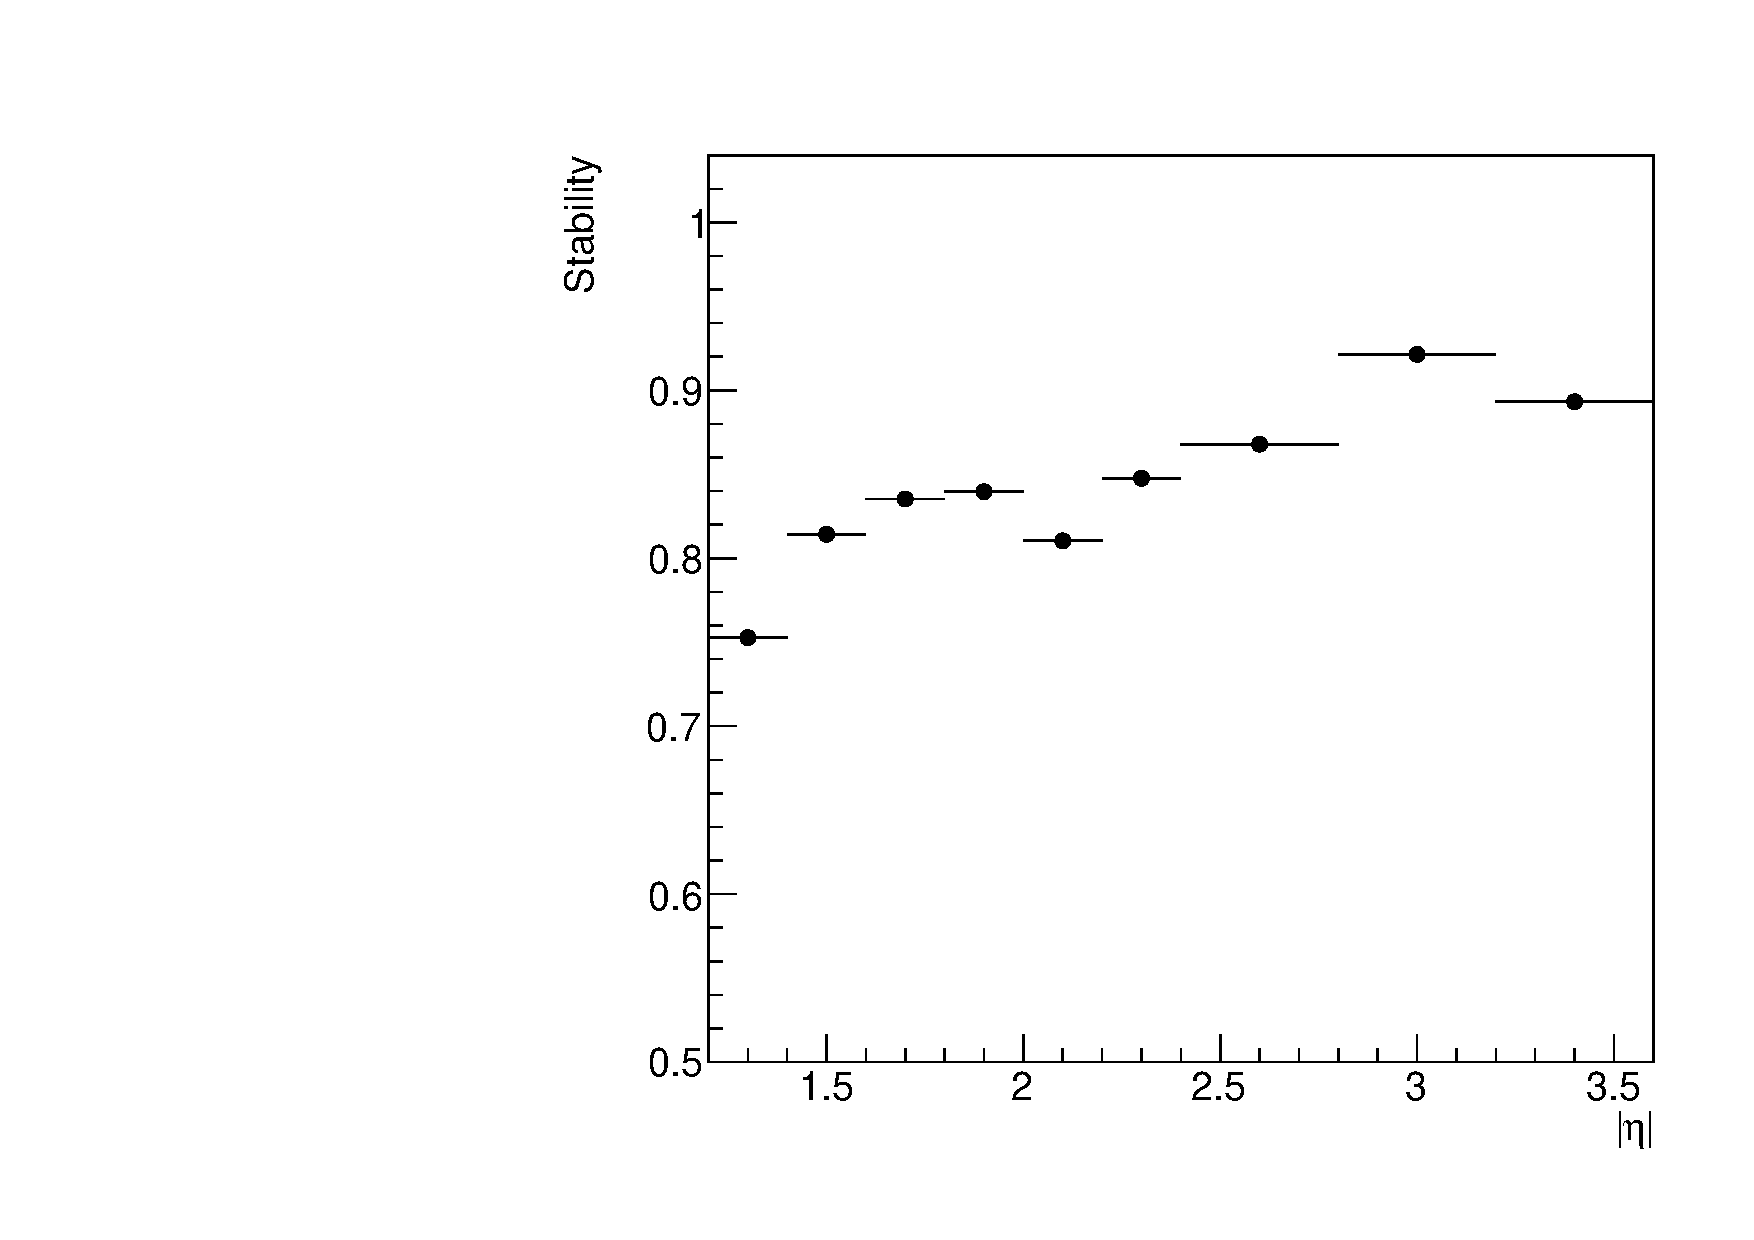
\includegraphics[width=0.45\textwidth]{figures/ZCF_stability_peak} \\
  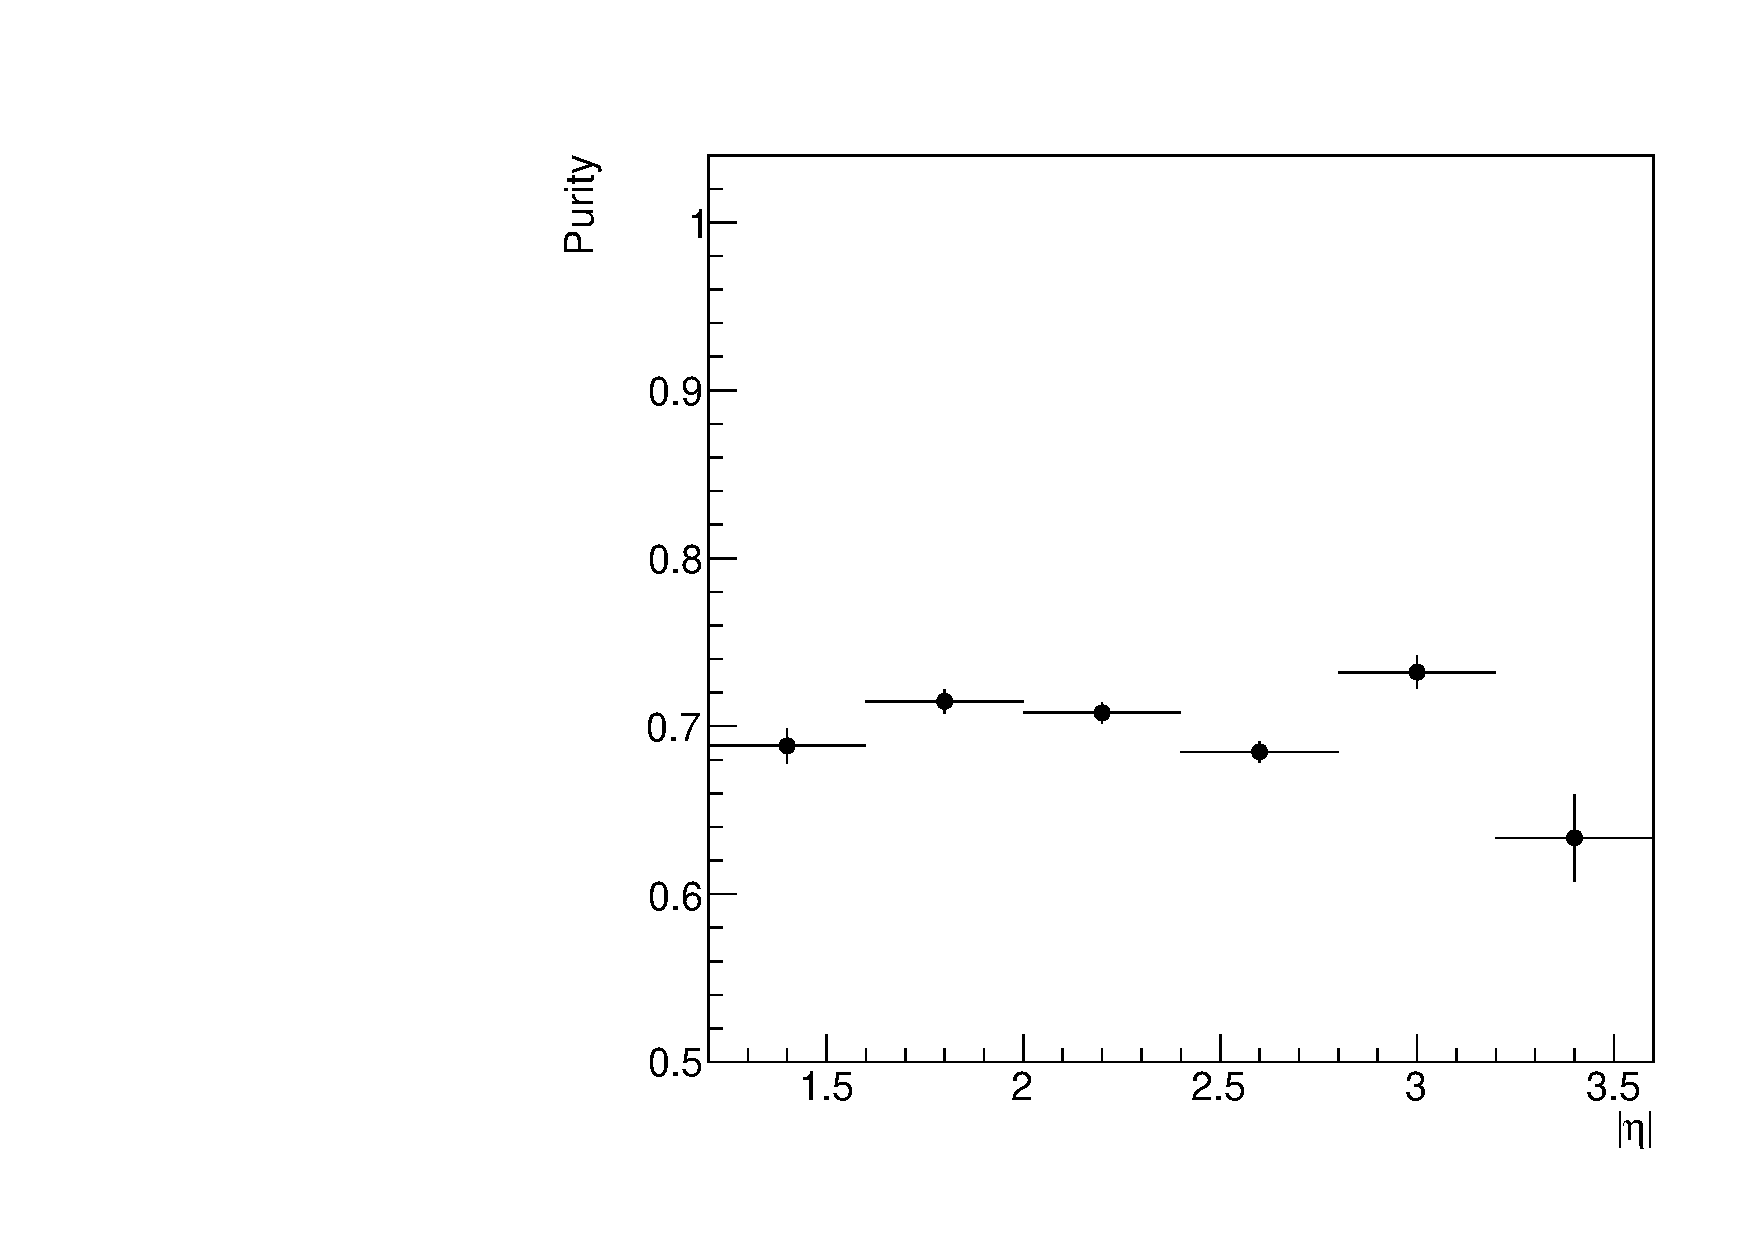
\includegraphics[width=0.45\textwidth]{figures/ZCF_purity_high}
  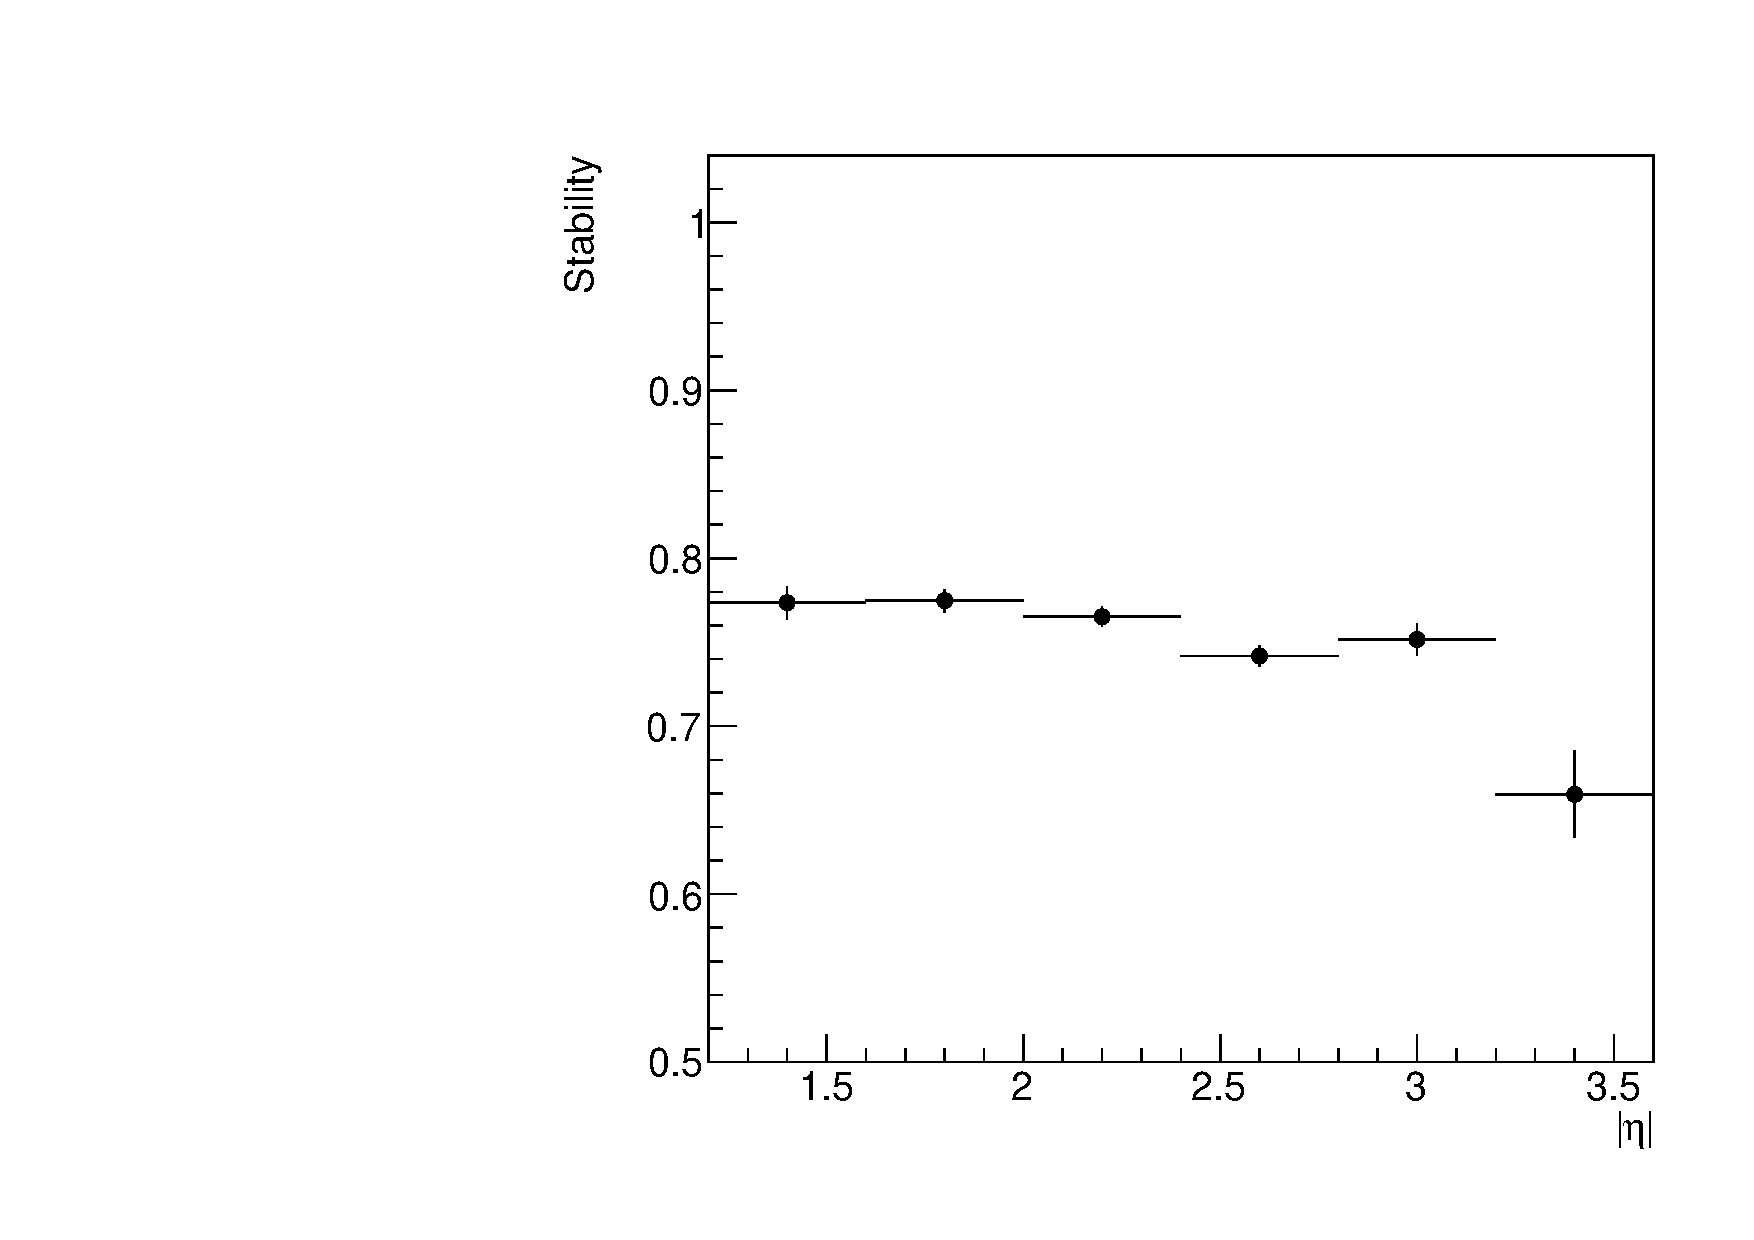
\includegraphics[width=0.45\textwidth]{figures/ZCF_stability_high} \\
  \caption{Purity (left) and stability (right) for the Z central-forward peak mass (top) and high mass (bottom) analyses.}
  \label{fig:ZeeCS_purity_stability}
\end{figure}

The differential cross-section measurement was done in absolute rapidity binning.
The binning is the same for CC and CF analyses in the region that is covered with both of them, which allows for the easy combination of the results. The binning is shown in Tabs.~\ref{tab:ZeeCS_bins_peak} and~\ref{tab:ZeeCS_bins_high}. The mass binning for the double-differential CF analysis had only two bins: the peak-mass window $66 < m_{ee} < 116$~GeV and the high-mass window $116 < m_{ee} < 150$~GeV.

\begin{table}
\centering
\begin{tabular}{c}
\hline\hline
Boundaries\\\hline
$1.20 < |y_{Z}| <1.40$\\
$1.40 < |y_{Z}| <1.60$\\
$1.60 < |y_{Z}| <1.80$\\
$1.80 < |y_{Z}| <2.00$\\
$2.00 < |y_{Z}| <2.20$\\
$2.20 < |y_{Z}| <2.40$\\
$2.40 < |y_{Z}| <2.80$\\
$2.80 < |y_{Z}| <3.20$\\
$3.20 < |y_{Z}| <3.60$\\
\hline\hline
\end{tabular}
\caption{Bins in $|y_{Z}|$ which are used for the \Zee\ CF analysis for peak mass window ($66 < m_{ee} < 116$~GeV).}
\label{tab:ZeeCS_bins_peak}
\end{table}

\begin{table}
\centering
\begin{tabular}{c}
\hline\hline
Boundaries\\\hline
$1.20 < |y_{Z}| <1.60$\\
$1.60 < |y_{Z}| <2.00$\\
$2.00 < |y_{Z}| <2.40$\\
$2.40 < |y_{Z}| <2.80$\\
$2.80 < |y_{Z}| <3.20$\\
$3.20 < |y_{Z}| <3.60$\\
\hline\hline
\end{tabular}
\caption{Bins in $|y_{Z}|$ which are used for the \Zee\ CF analysis for high mass window ($116 < m_{ee} < 150$~GeV).}
\label{tab:ZeeCS_bins_high}
\end{table}

\section{Bin-by-bin unfolding}
\label{sec:ZCS_bbb_unf}

The bin-by-bin unfolding doesn't take into account the migrations between bins, and works with every bin separately. The unfolded value can be then translated into the cross-section value, and the formulae for both integrated and differential cross-sections are:
\begin{equation}
\sigma_{tot} = \sigma_{Z} \times BR(\Zee) = \frac{N - B}{C \cdot E \cdot A \cdot L_{int}  \cdot \Gamma}\,,
\end{equation}
where:
\begin{itemize}
\item {\bfseries $N$} is the number of candidate events measured in data.
\item {\bfseries $B$} is the number of background events (see Section~\ref{sec:Bkg} for further information on the background estimation).
\item {\bfseries $L_{int}$} is the integrated luminosity corresponding to the dataset.
\item {\bfseries $\Gamma$} is the bin width for differential measurements. Measurements in rapidity quantities $\eta$ and $y$ are done in absolute binning as final value, therefore $\Gamma$ for them is doubled.
\item $C$, $E$, and $A$ are efficiency-acceptance corrections calculated from (binned) sum of weights of MC events generated or reconstructed with analysis cuts applied. They take the uncorrected event yield in steps to different levels:
\begin{itemize}
\item The coefficient for a \textit{genuinely experimental fiducial volume in each channel} as defined by the individual cuts is reached after dividing by
\begin{equation}
  C = \frac{N_\mathrm{MC, rec}}{N_\mathrm{MC, gen, cutexp}}\,.
\end{equation}
$C$ is corrected for any discrepancy in the electron efficiencies between data and MC as described in Section~\ref{sec:Efficiency}. Here the sum of weights of MC events generated after experimental fiducial acceptance cuts ($N_\mathrm{MC, gen, cutexp}$) and the sum of weights of MC events after simulation, reconstruction and experimental selection ($N_\mathrm{MC, rec}$) enter.
\item The coefficient for a \textit{common fiducial volume} is a theoretical extrapolation designed to unify the fiducial volumes of different flavors of \Zll\ analyses. Since the electrons and muons are detected by the different parts of the ATLAS detector, these particles are detected in different parts of the kinematic space. The EM calorimeters that detect electrons have a coverage of $|\eta| < 5.2$, while muon chambers have $|\eta| < 2.4$. These differences in the kinematic coverage makes combination of the results of corresponding analyses a big challenge. Therefore the common fiducial volume covering both kinematic spaces is introduced.
\begin{equation}
  E = \frac{N_\mathrm{MC, gen, cutexp}}{N_\mathrm{MC, gen, cutfid}}\,.
\end{equation}
Here the sum of weights of MC events generated after common fiducial acceptance cuts ($N_\mathrm{MC, gen, cutfid}$) enters.
\item The coefficient for a \textit{total cross sections} is calculated by a larger theoretical extrapolation
\begin{equation}
  A = \frac{N_\mathrm{MC, gen, cutfid}}{N_\mathrm{MC, gen, all}}\,.
\end{equation}
Here the total sum of weights of MC events generated before any acceptance cuts except $m_{ee}$ ($N_\mathrm{MC, gen, all}$) enters.
\end{itemize}
\end{itemize}


While calculating the $C$, $E$ and $A$ correction factors, the QED final state radiation (FSR) must be taken into account. The results of the MC generation are so-called {\itshape born level} leptons, which are the leptons before the FSR. To simulate FSR there are two tools in use in the MC production chain: \Photos\, which is the default tool used, and \Sherpa\ which uses another FSR algorithm and is used for systematic uncertainties evaluation. After the FSR simulation, the resulting final state leptons are called {\itshape bare leptons}. The bare leptons represent the result of the actual collision much closer than the born leptons, but because of the work of the clustering algorithms during reconstruction, bare leptons are impossible to reconstruct. To overcome this problem, another level of FSR was introduced, which is {\itshape dressed leptons}. The dressed leptons are bare leptons with the inclusion of all FSR photons within the $\Delta R < 0.1$. The dressed leptons are the leptons that most closely represent the particles that are actually reconstructed by the reconstruction algorithms.

The calculation of the correction factors is always done on the born level, because the simulation on the born level is the best from the theoretical point of view (the FSR simulation is very approximate). The $C$, $E$ and $A$ then look like this:
\begin{equation}
C = \frac{N_\mathrm{MC, rec}}{N_\mathrm{MC, genBorn, cutexp}}\,, \;
E = \frac{N_\mathrm{MC, genBorn, cutexp}}{N_\mathrm{MC, genBorn, cutfid}}\,, \;
A = \frac{N_\mathrm{MC, genBorn, cutfid}}{N_\mathrm{MC, genBorn, all}}\,.
\end{equation}
And for the bare and dressed levels the cross-sections are calculated with good approximation by using the $\delta^\mathrm{bare}$ and $\delta^\mathrm{dressed}$ which are defined as:
\begin{equation}
\begin{split}
  \delta^\mathrm{bare} = \frac{N_\mathrm{MC, genBare, fidcut}}{N_\mathrm{MC, genBorn, fidcut}}\:\:\:&\mbox{and}\:\:\:
  \delta^\mathrm{dressed} = \frac{N_\mathrm{MC, genDressed, fidcut}}{N_\mathrm{MC, genBorn, fidcut}}\\
  \sigma_{fid}^\mathrm{Born} \cdot \delta^\mathrm{bare} =
  \sigma_{fid}^\mathrm{bare} \:\:\:\:\:\:&\mbox{and}\:\:\:\:\:\:
  \sigma_{fid}^\mathrm{Born} \cdot \delta^\mathrm{dressed} =
  \sigma_{fid}^\mathrm{dressed} \,.
\end{split}
\end{equation}

In terms of unfolding matrix, the values $C$ calculated in each bin and corrected to the dressed level go into the diagonal positions of the $R^{-1}_{ij}$. The results unfolded with this matrix is called the {\itshape true experimental fiducial cross-section}. The additional extrapolation using the matrix constructed from the values $E$ will produce the {\itshape extrapolated fiducial cross-section}, and finally with the values $A$ we will get the {\itshape common fiducial cross-section} which can be used for the combination. The results for all of these cross-sections can be seen in Section~\ref{sec:Results}

\section{Bayesian (D'Agostini's) iterative unfolding}
\label{sec:ZCS_bay_unf}

The so-called Bayesian unfolding differs from the bin-to-bin unfolding in that it scales all the bins in a single pass, so the correlations between the different bins, as well as migrations, is better described. It is named after the Bayesian theorem for the conditional probability, which in case of cross-section unfolding can be presented as
\begin{equation}
P(C_i|E) = \frac{P(E|C_i) \, P(C_i)}{\sum\limits_l P(E|C_l) \, P(C_l)}
\end{equation}
where $C_i$ and $E$ are the {\itshape cause} and {\itshape effect}, where the effect would be an observed event reconstructed within certain bin, and the causes are the true events that happen in the certain bin. $P(C_i)$ is then the initial probability of the event to happen within the certain bin, and $P(E|C_i)$ is the conditional probability of said event to produce the effect (reconstructed particles). The formula may appear useless, as the initial probabilities $P(C_i)$ that participate in it are actually the very thing we are trying to calculate. But in reality, the values can be derived with the increasing number of observations, provided no assumptions were made on the values a priori. This iterative method of unfolding was developed by G. D'Agonini in 1995 and was since widely used by many experiments~\cite{lib:zcs_bayes}. The conditional probabilities $P(E|C_i)$ can be derived from MC simulations, and are constant throughout the observations (iterations). The different types of MC generators, though, can provide different values for those probabilities, and hence must be used to determine the boundaries of systematic uncertainties.

To describe the unfolding method, lets assume $n(E)$ the number of observed events with the effect $E$, and
\begin{equation}
\hat{n}(C_i) = n(E) \, P(C_i|E)
\end{equation}
is the true number of events with the cause $C_i$ that caused this effect. Since every cause $C_i$ can have several effects $E_j$, and the Bayesian formula holds for each of them, the probability $P(C_i|E_j)$ can be calculated as
\begin{equation}
P(C_i|E_j) = \frac{P(E_j|C_i) \, P_0(C_i)}{\sum\limits_l P(E_j|C_l) \, P_0(C_l)} \,.
\label{eq:zcf_p_ci_ej}
\end{equation}
Here the initial probability $P(C_i)$ was replaced with $P_0(C_i)$ to emphasize on the iterative nature of the method, which will be discussed later. Also it can be noted that $\sum_i P_0(C_i) = 1$ by definition, and $\sum_i P(C_i|E_j) = 1$ meaning that each effect must be produced by some cause. On the other hand, $\sum_j P(E_j|C_i)$ can be less than one, because a cause may produce no effect whatsoever, and hence this sum shows the efficiency of detecting the cause $C_i$ in any possible effect
\begin{equation}
\epsilon_i = \sum\limits_j P(E_j|C_i) \,.
\end{equation}
With this, the true number of events can be estimated as
\begin{equation}
\hat{n}(C_i) = \frac{1}{\epsilon_i} \, \sum\limits_j n(E_j) \, P(C_i|E_j)\;\;\; \epsilon_i \neq 0\,, \;\;\;
\hat{N}_\mathrm{true} = \sum\limits_i \hat{n}(C_i)
\end{equation}
where $P(C_i|E_j)$ is calculated from Eq.~(\ref{eq:zcf_p_ci_ej}). From here, the values for the unfolding matrix can be calculated as
\begin{equation}
P(C_i) = \frac{\hat{n}(C_i)}{\hat{N}_\mathrm{true}}\,.
\end{equation}
The iterative unfolding procedure then goes as follows:
\begin{enumerate}
\item Pick an initial unbiased $P(C_i)$ distribution from the best knowledge of the unfolded process so that $n(C_i) = P(C_i)\,N_\mathrm{obs}$. The uniform distribution can also work.
\item Calculate the next iteration of $\hat{n}(C_i)$ and $P(C_i)$ based on the previous distribution.
\item Make a $\chi^2$ comparison between $\hat{n}(C_i)$ distributions before and after the iteration.
\item If $\chi^2$ is not satisfactory, repeat from step 2.
\end{enumerate}
The optimal number of the iterations depends on the statistical errors of the initial data. With infinite statistics, the number of iteration is not restricted by anything, and sufficiently big number of iteration will produce the true distribution with any precision. But for finite number of events, the number of iteration should be relatively small, as in the extreme case of infinite iterations, the resulting unfolding matrix equals to the inverted detector response matrix, which defies the whole purpose of the Bayesian method. But because of the quick convergence, even the first iteration results in the distribution which is close to the true. Usually, two to three iterations are chosen for the data unfolding.

For the uncertainty propagation the ToyMC method is used (see Section~\ref{sec:ZeeD_toymc}).

\section{Combination of the several cross-sections}
\label{sec:ZeeCS_comb}

When calculating the cross-section for \Zll\ decay, there are several independent channels from which the data is acquired. And the results produced from different sources overlap in some parts of the kinematic space. In theory, the calculated cross-section should be the same for all channels, but since the results come with uncertainties, it's not always the case. Let's assume that some value was measured as $\mu$ with the uncertainty of $\Delta$. Assuming that the uncertainty is gaussianely shaped, the probability distribution for the true value $m$ can be written as
\begin{equation}
P(m) = \frac{1}{\sqrt{2\pi\Delta}}\exp\left(-\frac{(m-\mu)^2}{2\Delta^2}\right) \,,
\end{equation}
and the corresponding $\chi^2$ function would be
\begin{equation}
\chi^2(m) = \frac{(m-\mu)^2}{\Delta^2} \,.
\end{equation}
When there are several measurements of the same true value $(\mu_1, \Delta_1)$, $(\mu_2, \Delta_2)$ and so on, the combined probability function will be
\begin{equation}
P_\mathrm{comb}(m) \sim \exp\left(-\frac{(m-\mu_1)^2}{2\Delta_1^2}\right) \cdot \exp\left(-\frac{(m-\mu_2)^2}{2\Delta_2^2}\right) \cdot ...
\end{equation}
with the combined $\chi^2$ being the sum if the individual ones $\chi^2_\mathrm{sum} = \chi^2_1 + \chi^2_2 + ...$. So if we are to replace the multitude of measurements with a single average one, we are to rewrite the combined $\chi^2$ in the form of
\begin{equation}
\chi^2_\mathrm{comb}(m) = \frac{(m-\mu_\mathrm{ave})^2}{\Delta_\mathrm{ave}^2} + \chi^2_0\,,
\end{equation}
where $\mu_\mathrm{ave}$, $\Delta_\mathrm{ave}$ and $\chi^2_0$ can be found from
\begin{equation}
\mu_\mathrm{ave} = \argmin_m \chi^2_\mathrm{sum}(m) \:,\:\: \chi^2_0 = \chi^2_\mathrm{sum}(\mu_\mathrm{ave}) \:,\:\:\Delta_\mathrm{ave}: \chi^2_\mathrm{sum}(\mu_\mathrm{ave}\pm\Delta_\mathrm{ave})=\chi^2_0+1 \,.
\end{equation}
The $\chi^2_0$ shows the consistency of measurements, and for measurements to be consistent the relation $\chi^2_0 / N_\mathrm{DoF} \approx 1$ must hold true.

The same technique applies in case of measurements made in several bins, but only if the bins are fully independent, i.e. the uncertainties are fully uncorrelated. In case of the uncertainties correlated between bins, the calculation of the combined values becomes more complex. The systematic uncertainties also can be regarded as a results of experiments, and as such have a true and measured values and an uncertainty of its own with a similar relation $\chi^2_\mathrm{syst}=(\alpha - \alpha_0)^2/\Delta^2_\alpha$. While we usually are unable to calculate $\alpha$ and $\Delta_\alpha$, it is not needed, since the covariance matrix decomposition which we do during the systematic uncertainty unfolding provide us with the nuisance parameters $b_s = (\alpha_s - \alpha_{0,s})/\Delta_{\alpha,s}$. With this in mind, the equation for $\chi^2$ would look like
\begin{equation}
\chi^2(m,\vec{b}) = \sum\limits_i \frac{\left(m-\mu_i - \sum\limits_s \Gamma^s_i b_s\right)^2}{\Delta^2_i}+\sum\limits_s b^2_s \,,
\end{equation}
where $i$ runs over all the combined measurements and $s$ runs over all the sources of the correlated systematic uncertainties, $\vec{b}$ is composed of the nuisance parameters $b_s$, $\Delta_i$ is an uncorrelated and $\Gamma_{s,i}$ is correlated uncertainties.

For the combination of the several measurements with the same binning the combined $\chi^2$ is not equal to direct sum of the individual ones, since all the measurements usually share some sources of the systematic uncertainties, so the instead of a direct sum, the $\chi^2_\mathrm{sum}$ would look as such
\begin{equation}\label{eq:chi2_sum_multi}
\chi^2_\mathrm{sum}(\vec{\vphantom b\smash{m}},\vec{b}) = \sum\limits_k\sum\limits_i \frac{\left(m_k-\mu_{k,i} - \sum\limits_s \Gamma^s_{k,i} b_s\right)^2}{\Delta^2_{k,i}} W_{k,i}+\sum\limits_s b^2_s \,,
\end{equation}
where $k$ runs over all bins, $s$ runs over all sources of the systematic uncertainties for all measurements, and $m_k$ substitute $\vec{m}$. $W_{k,i}$ is equal to $1$ if the measurement $i$ contributes to the bin $k$, and $0$ otherwise. If the source $k$ is insensitive to the source $s$ of the systematic uncertainty, then $\Gamma^s_k$ is equal to $0$. The multibinned version of the combined $\chi^2_\mathrm{comb}$ is constructed the same way as before
\begin{equation}
\begin{gathered}
\chi^2_\mathrm{comb}(\vec{\vphantom b\smash{m}},\vec{b}) = \sum\limits_k\frac{\left(m_k-\mu_{k,\mathrm{ave}}-\sum\limits_s \Gamma^s_{k,\mathrm{ave}}(b_s - b_{s,\mathrm{ave}})\right)^2}{\Delta_{k,\mathrm{ave}}^2} \\
+ \sum\limits_{k_1} \sum\limits_{k_2} (b_{k_1} - b_{s,\mathrm{ave}})(b_{k_2} - b_{s,\mathrm{ave}})(A'_S)_{k_{1}k_{2}} + \chi^2_0\,.
\end{gathered}
\end{equation}
The values $\vec{\vphantom b\smash{\mu}}_\mathrm{ave}$, $\vec{b}_\mathrm{ave}$ and the matrix $A'_S$ can be found from the minimization of the Eq.~(\ref{eq:chi2_sum_multi}) with respect to the variables $m_k$ and $b_s$, which can be expressed in the form of partial derivatives $\partial\chi^2_\mathrm{sum}/\partial m_k = 0$, $\partial\chi^2_\mathrm{sum}/\partial b_s = 0$ or in the matrix form
\begin{equation}
\left( \begin{array}{cc} \vphantom{\vec{b}}  A_M & A_{SM} \\ \vphantom{\vec{b}}(A_{SM})^T & A_S \end{array} \right)
\left( \begin{array}{c}  \vphantom{\vec{b}}\vec{\mu}_\mathrm{ave} \\ \vec{b}_\mathrm{ave} \end{array} \right)
=
\left( \begin{array}{c} \vphantom{\vec{b}}\vec{c}_M \\ \vphantom{\vec{b}}\vec{c}_S \end{array} \right) \,,
\end{equation}
where
\begin{itemize}
\item $A_M = \underset{k}{\mathrm{diag}}\left(\sum\limits_i\frac{W_{k,i}}{\Delta^2_{k,i}}\right)$
\item $A^{ks}_{SM} = - \sum\limits_i\frac{\Gamma^s_{k,i}}{\Delta^2_{k,i}}W_{k,i}$
\item $A^{s_{1}s_{2}}_{S} = \delta_{s_{1}s_{2}} + \sum\limits_k \sum\limits_i \frac{\Gamma^{s_1}_{k,i}\Gamma^{s_2}_{k,i}}{\Delta^2_{k,i}} W_{k,i}$
\item $c^k_M = \sum\limits_i \frac{\mu_{k,i}}{\Delta^2_{k,i}}W_{k,i}$
\item $c^s_S = - \sum\limits_k \sum\limits_i \frac{\mu_{k,i}\Gamma^s_{k,i}}{\Delta^2_{k,i}} W_{k,i}$
\end{itemize}
In all of the above $i$ runs over all measurements, $k$ runs over all bins and $s$ runs over all the systematic uncertainty sources. The final values for the combined results can thus be found as
\begin{equation}
\begin{aligned}
A'_S &= A_S - (A_{SM})^T A^{-1}_M A_SM \\
\vec{b}_\mathrm{ave} &= (A'_S)^{-1}\left(\vphantom{\vec{b}}\vec{c}_S - (A_{SM})^T A^{-1}_M \vec{c}_M\right) \\
\vec{\mu}_\mathrm{ave} &= A^{-1}_M \left(\vec{c}_M - A_{SM}\vec{b}_\mathrm{ave}\right) \,.
\end{aligned}
\end{equation}
The values for the statistical and uncorrelated systematical uncertainty can be found as
\begin{equation}
\Delta_{k,\mathrm{ave}}^2 = \frac{1}{A^{kk}_M} = \frac{1}{\sum\limits_i\frac{W_{k,i}}{\Delta^2_{k,i}}} \,.
\end{equation}

\chapter{Efficiency calculations}
\label{sec:Efficiency}

The reconstruction steps described in the Section~\ref{sec:Reconstruction} are not absolutely effective. The algorithms occasionally misinterpret particles and thus introduce the errors in the results. This margin of error is called the efficiency, and it is present for reconstructing both collision and MC samples. But to be able to compare collision data to theoretical predictions, the efficiency in both cases should be the same, which is not the case. To remedy this, the so-called "efficiency correction factors" were introduces for every step of the reconstruction chain: for trigger efficiency ($\varepsilon_\mathrm{TG}$), reconstruction efficiency ($\varepsilon_\mathrm{Reco}$), identification efficiency ($\varepsilon_\mathrm{ID}$), and isolation efficiency ($\varepsilon_\mathrm{ISO}$). The correction factor for every efficiency is defined as a ratio $\varepsilon^\mathrm{data}/\varepsilon^\mathrm{MC}$.

All efficiencies are measured using the tag-and-probe method, which require two electrons, one of which should pass the tight identification and would be called "tag", and the other should pass the weak identification and would be called "probe". If the "probe" also passes the tight identification, it is called "passing probe", and it is called "failing probe". The efficiency is then calculated as a ratio of the passing probes to the whole amount of tags, and is usually calculated in 2D binning of $|\eta|$ and \pt.

In the following sections all the efficiencies would be discussed separately.

\section{Trigger efficiency}

The efficiency of the electron triggers was determined with the help of the \Zee\ data which gives a clear selection of electrons with wide range in both \pt\ and $\eta$. For the central-forward analysis one uses a single-electron trigger, but since we need two electrons for the tag-and-probe method, the trigger efficiency was calculated using the central-central \Zee\ data. To get that data, the usual \Zee\ CC cut chain was applied, but with identification (ID) and isolation (ISO) cuts being changed to that, required from the central electrons from the \Zee\ CF and \Wenu\ analyses. After that every electron was consecutively used as a "tag" and as a "probe", with the "tag" always being required to be matched to the single-electron trigger, and the efficiency of a successful match of the "probe" to the same trigger being evaluated.

The scale factors were calculated in three different mass windows of $70 \le m_{ee} \le 110$~GeV, $80 \le m_{ee} \le 100$~GeV, and $85 \le m_{ee} \le 95$~GeV, to vary the background level. The results from the middle mass window were used to define the central value of the scale factors, while the other two were used to derive a source of uncertainty. To evaluate the uncertainty further, a background subtraction via OS-SS pairs (opposite sign minus same sign) was performed. The central value was taken from the OS pairs and the full difference to the OS-SS sample was taken as another source of uncertainty.

The whole MC sample was divided into four periods, corresponding to data periods B-H, I-J, K and L-M. Each of these MC periods is distinguishable by its unique LAr calorimeter and trigger setups, and should be used separately in order to calculate the scale factors which are valid only for that particular period. After propagation to the final cross section measurement using the combined ToyMC method (see Section~\ref{sec:ZeeD_toymc}), the resulting uncertainty is typically $0.1\%$ only.

The calculated trigger efficiencies as function of $\pt$ and $\eta$ for the default single-electron triggers used in the analysis are presented in Figure~\ref{fig:eff_trig}.

\begin{figure}
\center{
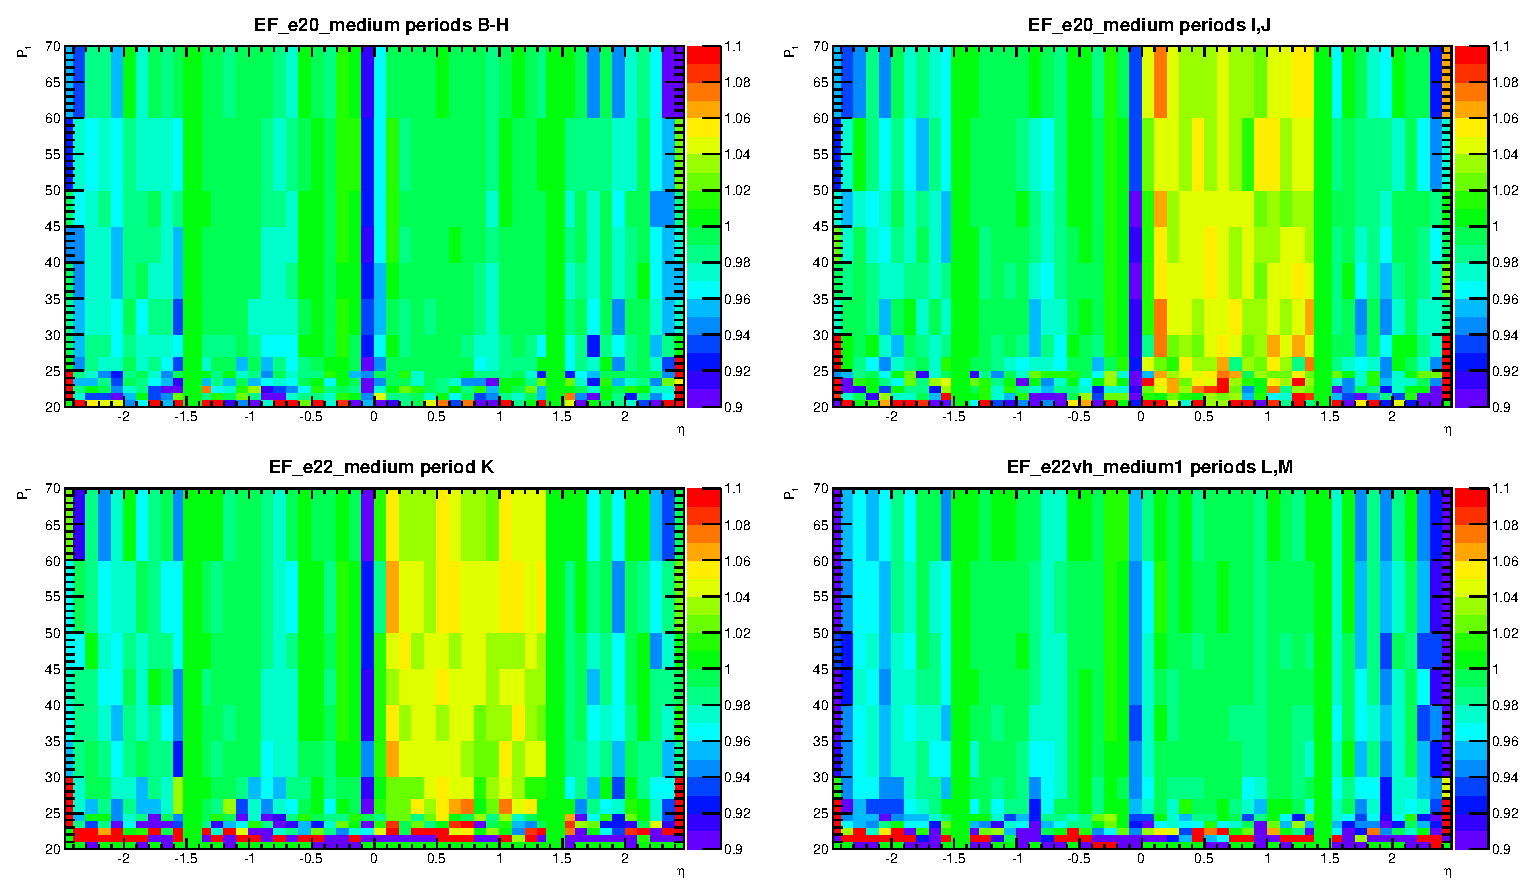
\includegraphics[width=1.0\textwidth]{figures/SingElTrigSFs2D.eps}
\caption{Scale factors for the default single-electron triggers used in the 2011 data. The plots were made using the \Zee\ MC samples with standard CC analysis cuts with the additional requirements on electron ID and ISO from the CF analysis.}
\label{fig:eff_trig}}
\end{figure}

\section{Reconstruction and identification efficiency}

There are three separate efficiencies that contribute to the electron identification: the efficiency of the cluster reconstruction algorithm, the efficiency of the electron reconstruction algorithm, and the efficiency of the electron identification algorithm. Every subsequent algorithm only works if its predecessors succeeded, so all the three efficiencies are tied together, and may be explored together.

\subsection{Central electron identification efficiencies}

For the central electrons, the samples from the \Zee, \Wenu, and $J/\psi \to ee$ were taken in the kinematic intervals of $7 < \et < 50$~GeV and $|\eta| < 2.47$~\cite{lib:elec_reco}. The efficiencies and uncertainties were calculated separately for each channel, and then combined for the calculation of the scale factors to reduce the uncertainties. For all three channels the selection for the tag electron required it to be reconstructed inside the $|\eta| < 2.47$ range with at least six hits in the SCT and at least one hit in the pixel detector. Tight selection criteria are applied to the tag object, which is an electron in case of \Zee\ and $J/\psi \to ee$ events, and is a $\et^{miss}$ in case of \Wenu. To further decrease the amount of background, additional cuts were applied to each channel separately.

For the \Wenu\ channel the selection was tighten for the lower-mass events, i.e. the ones with the transverse energy $40 < \et < 50$~GeV and missing transverse energy $25 < \et^{miss} < 40$~GeV. For the tighter selection, the probe electron was required a $\pt > 15$~GeV, and the event was discarded if more then one electron candidate satisfied the medium ID criteria. To reduce the amount of hadrons misidentified as electrons, two additional isolation criteria were added: the probe electron should be separated from any jet with $\pt > 25$~GeV with a cone of at least $\Delta R > 0.4$, and similarly the $\et^{miss}$ vector should be separated from any jet with the same energy by the angular distance of at least $\Delta \varphi > 0.7$.

For the \Zee\ channel the additional criteria included the $\et > 20$~GeV cut for the tag electron, as well as exclusion of the transition region $1.37 < |\eta| < 1.52$, and similar to isolation requirement for the probe electron from the \Wenu channel: no jets with $\pt > 25$~GeV within the $\Delta R < 0.4$ cone. The OS cut was required for the selection, but the SS events were also counted for the OS-SS background substraction the same way as in the trigger efficiencies calculation. The mass window was tighten to $80 < m_{ee} < 100$~GeV to further suppress the background.

For the $J/\psi \to ee$ channel the additional filtering was very high due to more difficult reconstruction of the low \et\ events. There are two types of events in this channel: prompt and non-prompt. The event is called prompt when it happens in the vicinity of the primary vertex, while the non-prompt $J/\psi$ particles are displaced from the main vertex due to the relatively long lifetime of its parent $b$-hadron. The non-prompt events are usually surrounded by the hadronic activity which complicates the task of proper identification even further. To remedy this the events are split in two parts based on the lifetime of the $J/\psi$ parent particle derived from the transverse shift of the event vertex from the primary vertex, with events with longer lifetime being non-prompt. The additional restriction are also put on the tag electron, which requires additional TRT hits and large isolation cones.

For the evaluation of the remaining amount of background, the discriminating variables are used for each of the channels. For \Wenu\ the discriminating variable is the isolation: the sum of all energies from both electromagnetic and hadronic calorimeters is calculated for the cone around the probe electron, excluding the energy from the electron itself. The resulting quantity is then referred as $\et^{cone}(X)/\et$ where $X$ is $\Delta R$ of the cone, usually $0.3$. The background template is constructed by reversing the two criteria of the electron id: TRT high-threshold fraction from the tight ID, and the total shower width from the loose ID. The discriminating variable is used to determine which bins are more signal-dominated, and which are background-dominated (located below and above the threshold respectively), and then the template is fitted to data for the background-dominated bins, and scaled respectively for the signal-dominated ones. For the \Zee\ events there are two discriminating variables, and thus two background templates available. The first one is the $m_{ee}$ mass window, where the template is constructed from the events failing at least two loose ID cuts and with a significant amount of energy in a cone around the probe. The template is fitted to data in the high-energy mass window $m_{ee} > 120$~GeV. The second template is the same as for the \Wenu\ events. For the $J/\psi \to ee$ channel the same mass window is used as for \Zee\ channel. The template is constructed mainly from the same sign events with some additions made with Chebyshev polynomials.

\begin{figure}
\center{
\subfigure[\Wenu]{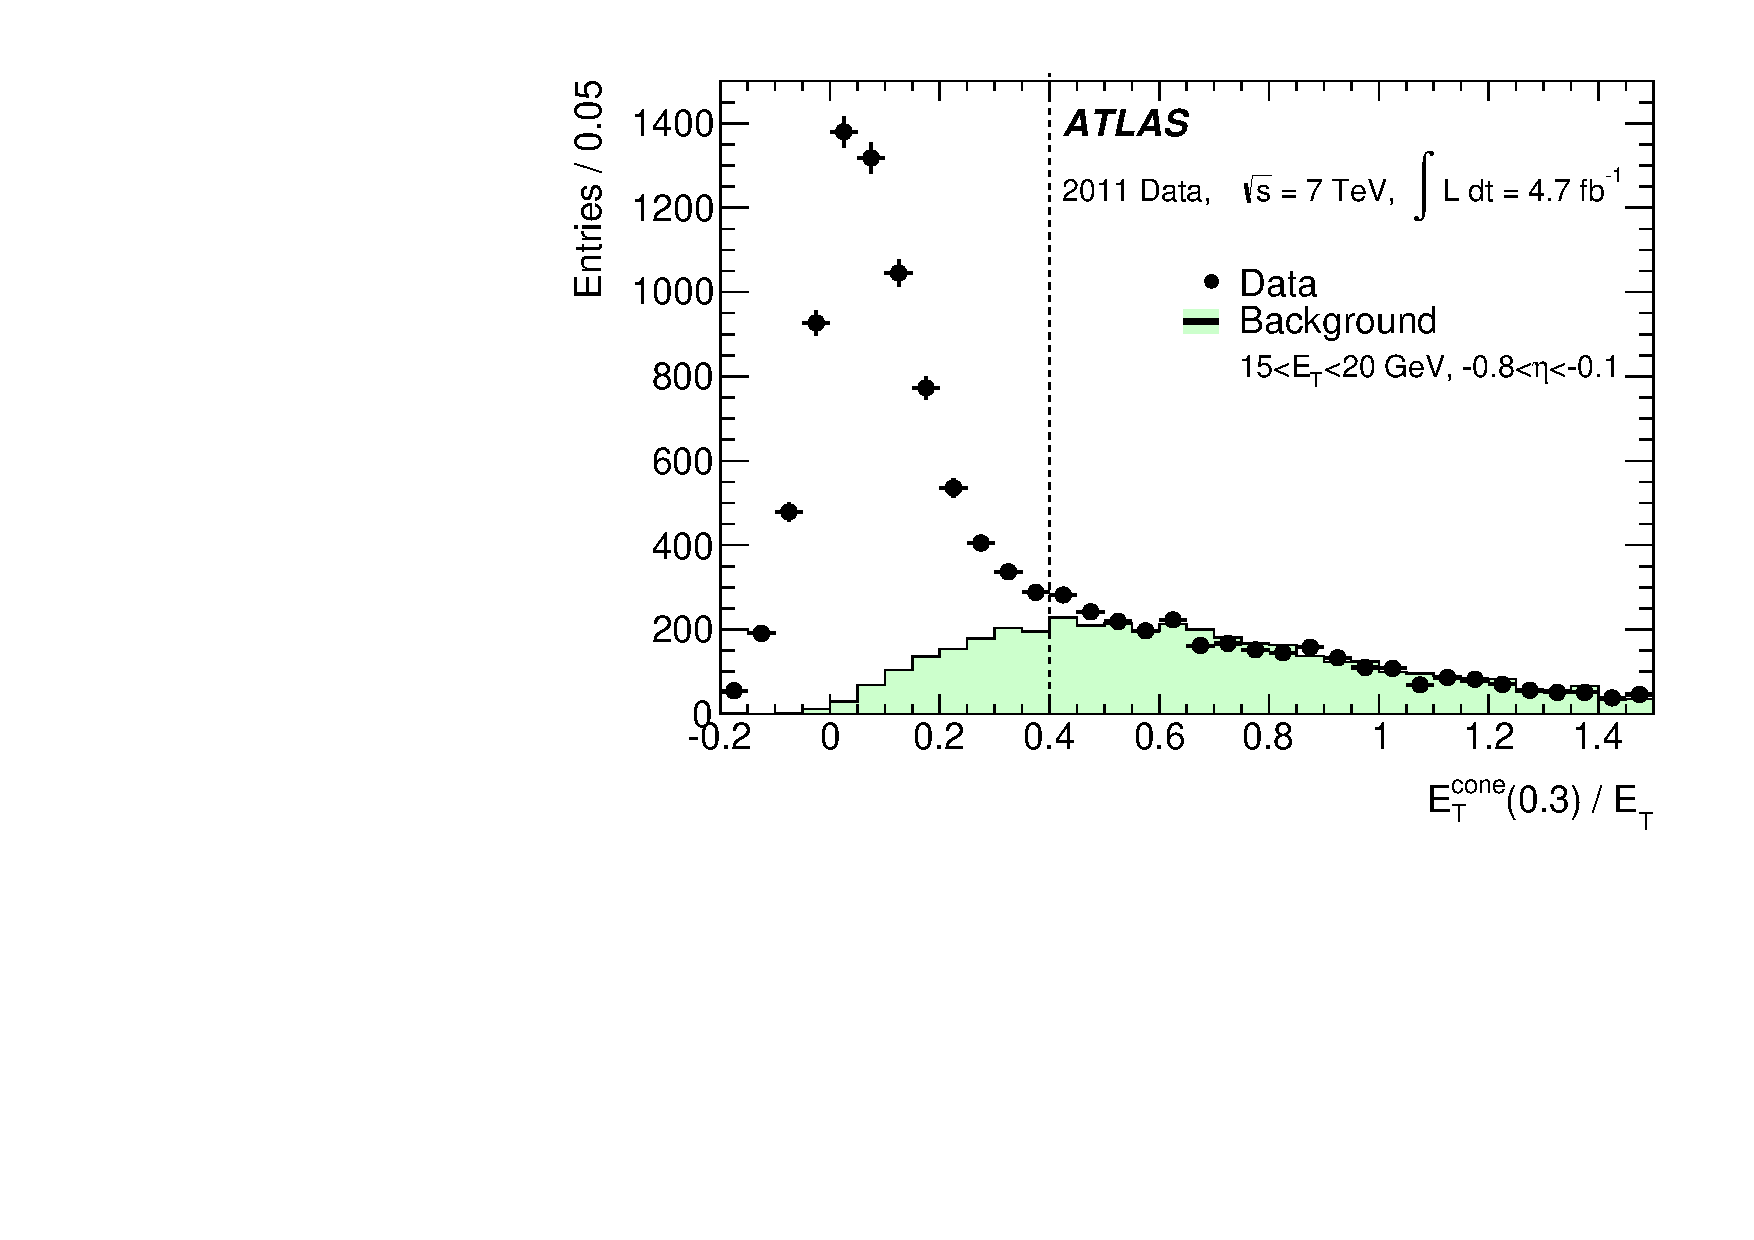
\includegraphics[width=0.45\textwidth]{figures/eff_rec_id_bg_a.pdf}}
\subfigure[\Zee]{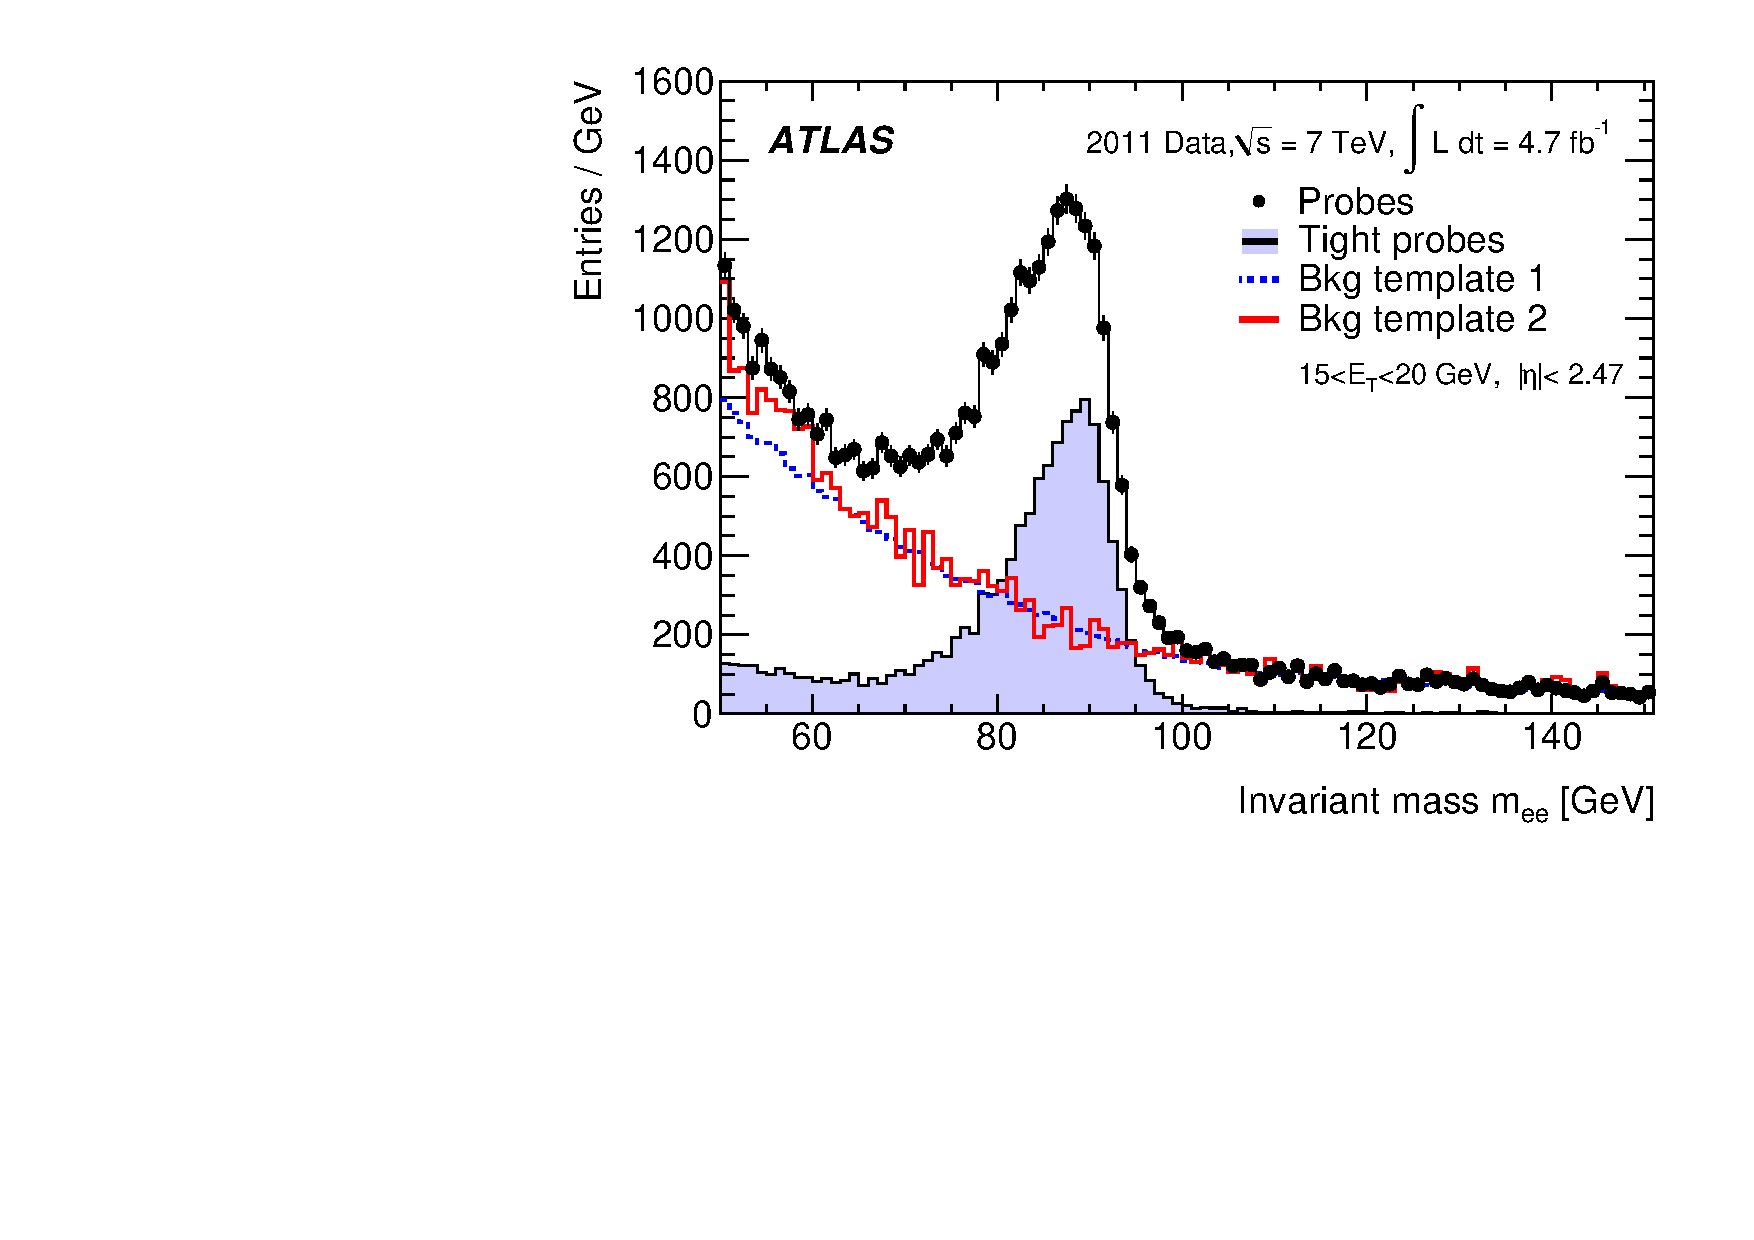
\includegraphics[width=0.45\textwidth]{figures/eff_rec_id_bg_b.pdf}}
\subfigure[$J/\psi \to ee$ prompt]{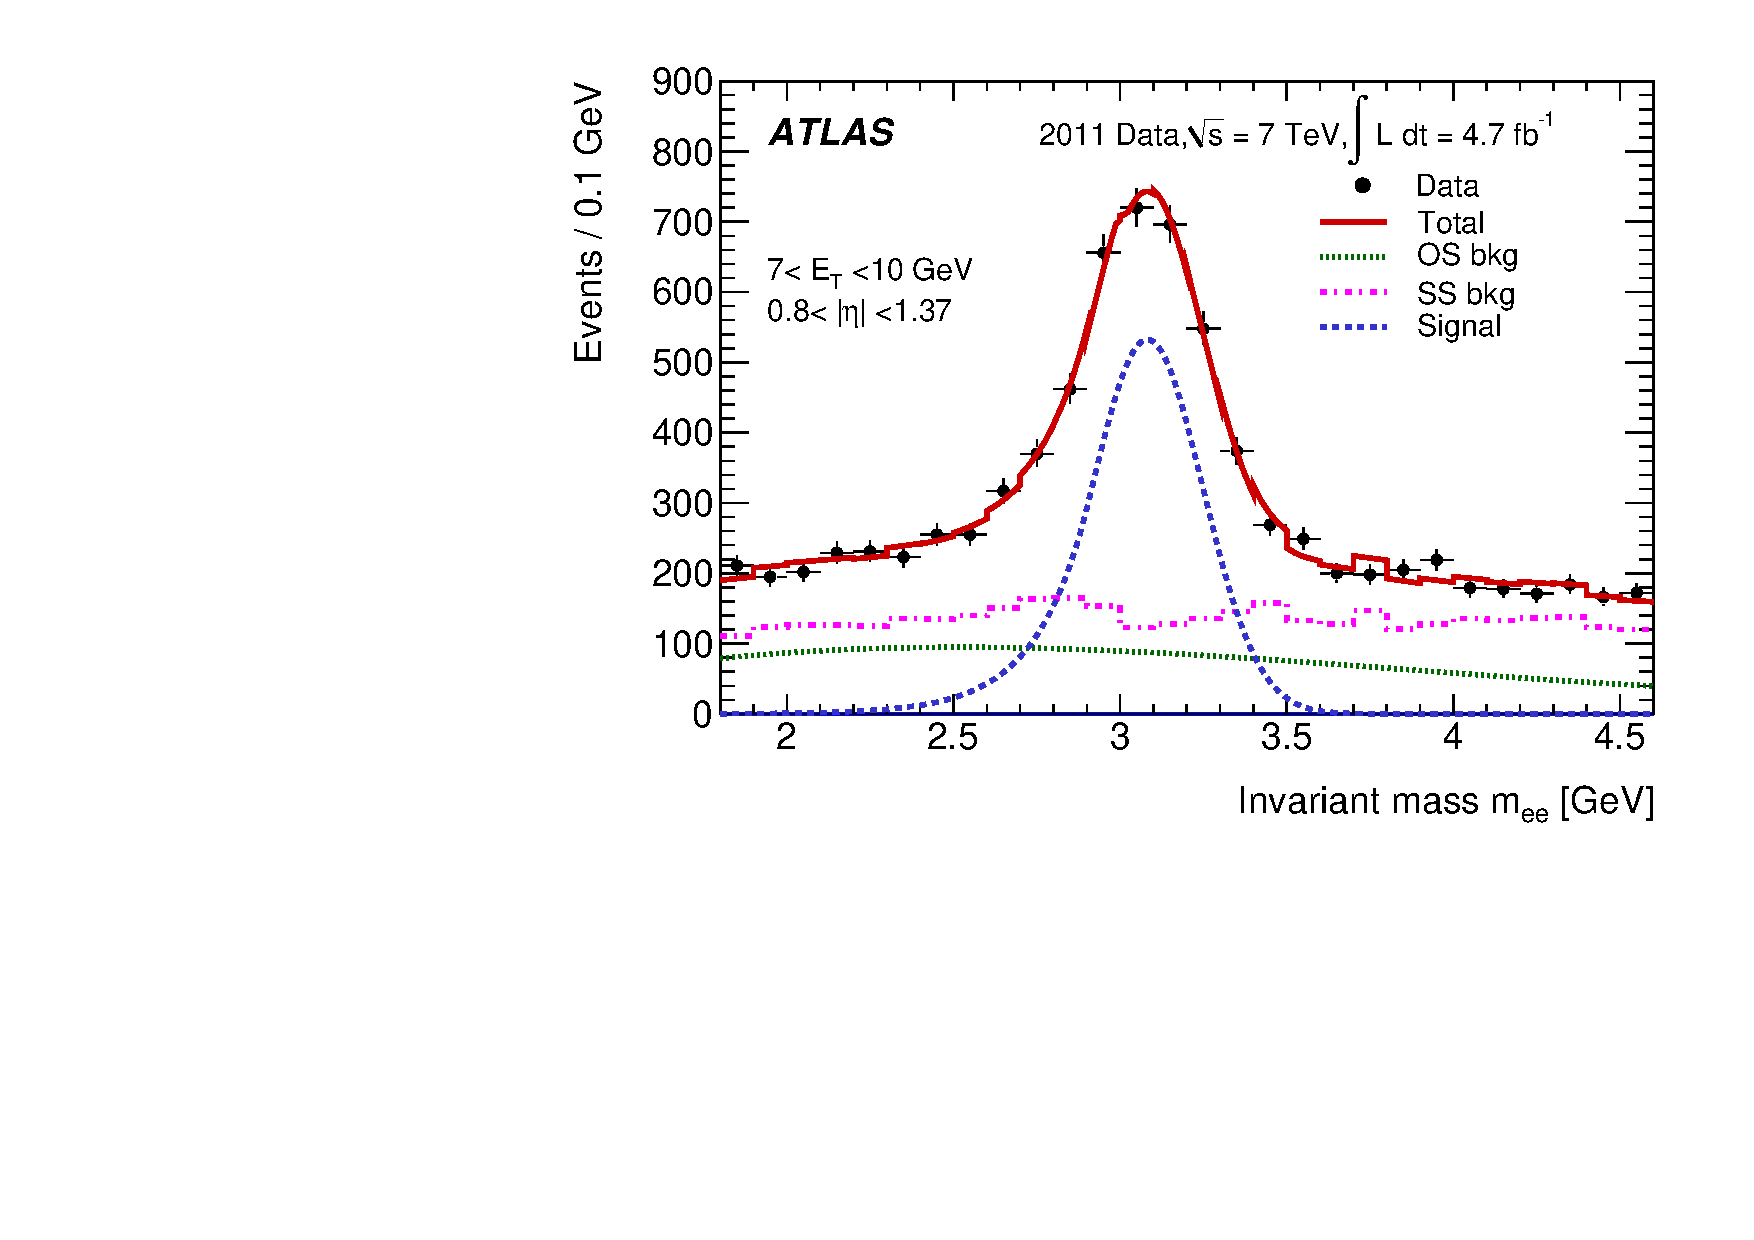
\includegraphics[width=0.45\textwidth]{figures/eff_rec_id_bg_c.pdf}}
\subfigure[$J/\psi \to ee$ non-prompt]{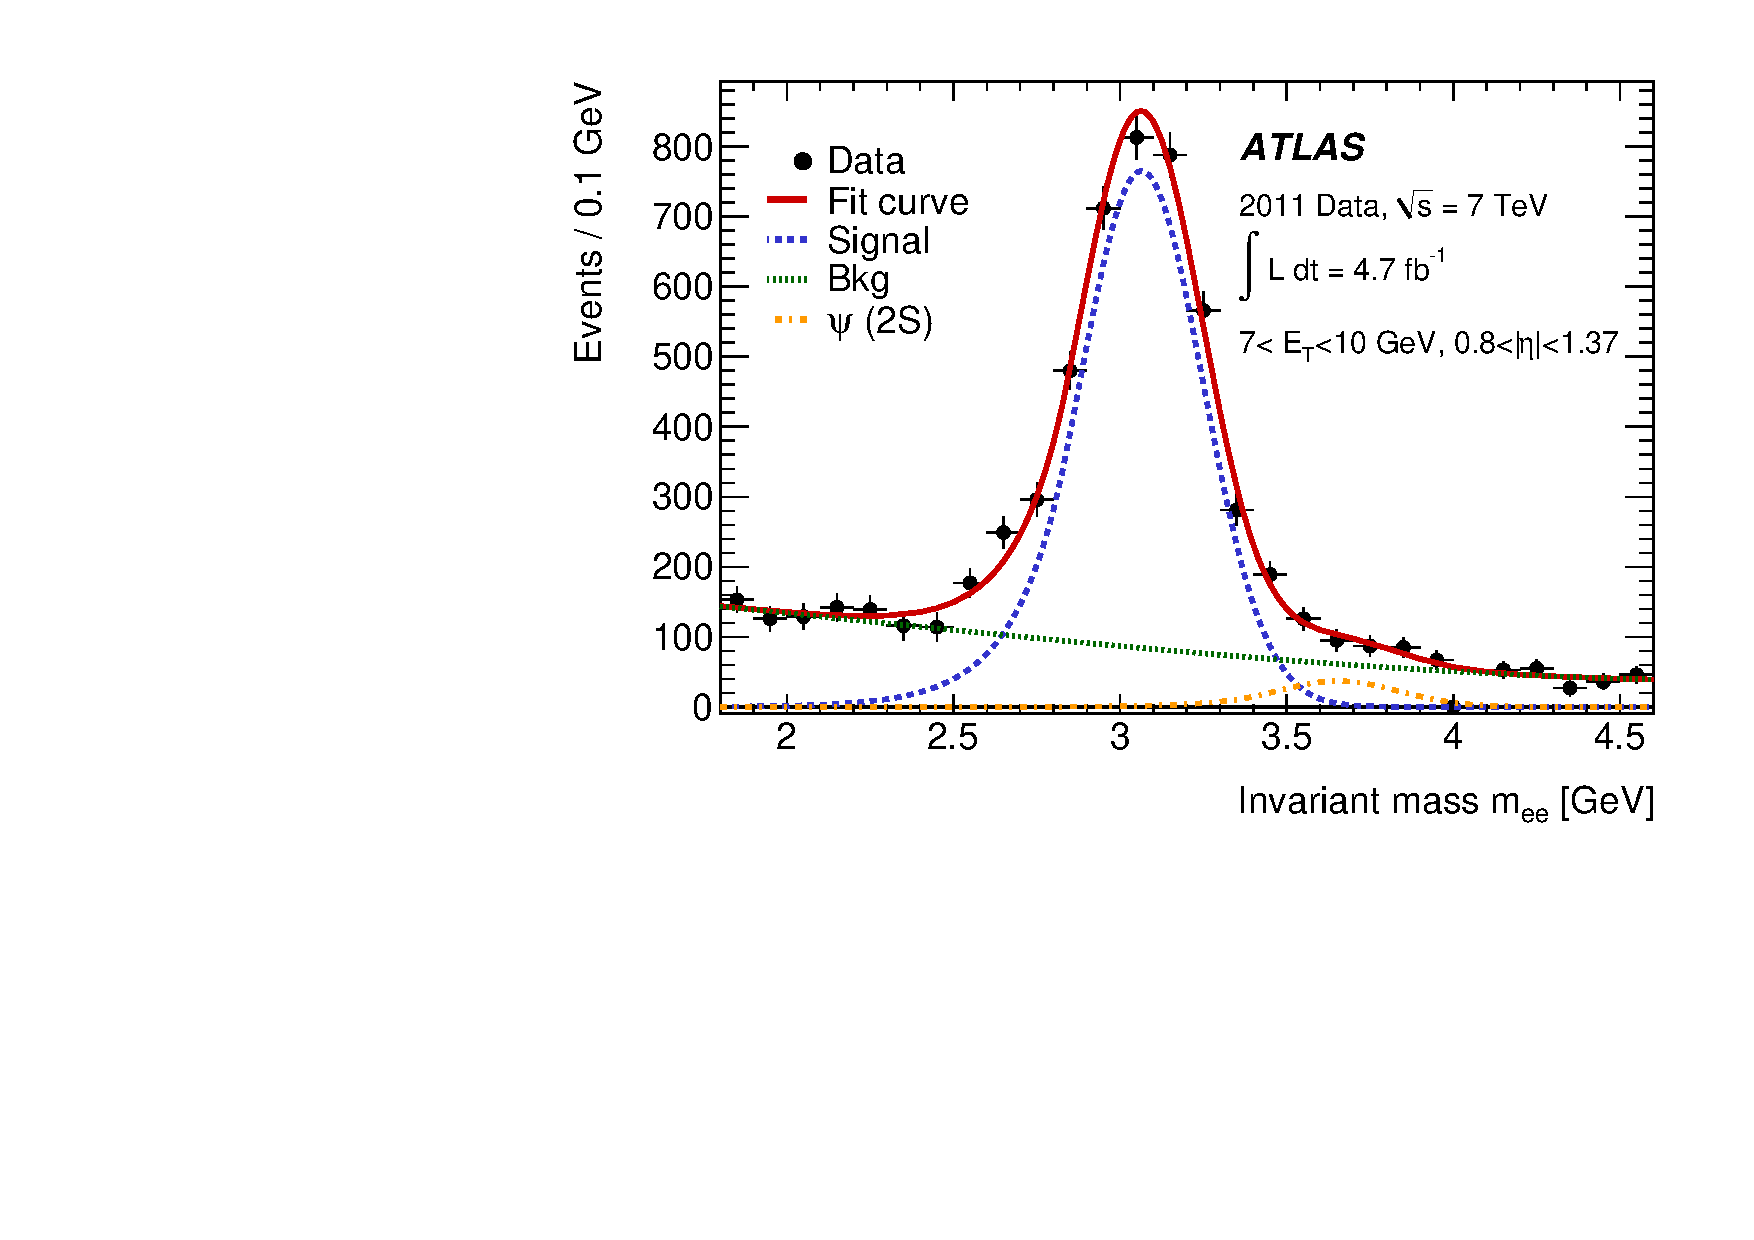
\includegraphics[width=0.45\textwidth]{figures/eff_rec_id_bg_d.pdf}}

\caption[Background estimation for different channels. (a) shows the $\et^{cone}(0.3)/\et$ variable of \Wenu\ events for probes (black dots) and normalized background template. The black dashed line shows the threshold. (b) shows two normalized background templates for \Zee, see text for details. (c) and (d) show backgrounds for short-lifetime (prompt) and long-lifetime (non-prompt) $J/\psi \to ee$ events respectively, being decomposed to various components.]{Background estimation for different channels. (a) shows the $\et^{cone}(0.3)/\et$ variable of \Wenu\ events for probes (black dots) and normalized background template. The black dashed line shows the threshold. (b) shows two normalized background templates for \Zee, see text for details. (c) and (d) show backgrounds for short-lifetime (prompt) and long-lifetime (non-prompt) $J/\psi \to ee$ events respectively, being decomposed to various components.~\cite{lib:elec_reco}}
\label{fig:eff_rec_id_bg}}
\end{figure}

For the uncertainties calculation, the shifting of various parameters is applied to all channels and the resulting shift in the efficiencies is observed. For the \Wenu\ events the thresholds for the $\et^{miss}$ and $m_{t}$ cuts are shifted, and the width of the cone for the discriminating variable is alternated to $0.4$. For the resulting $\sim$80 samples the backgrounds are then evaluated using the same method, and the resulting spread of the efficiencies is calculated. For the samples used the signal/background ratio distribution in the signal region exhibits an RMS (Root Mean Square) of 30\% at low \et\ (15-20~GeV) and 25\% at high \et\ (35-40~GeV). For the \Zee\ events the different mass-windows is used along with some alternative criteria for the tag electron. Both background templates are used, and in case of the isolation template the radius of the cone is also shifted, which gives in total about 120 samples. The S/B ratio distribution exhibits an RMS around 10\%. For the $J/\psi \to ee$ channel the isolation criteria was shifted for the tag electron as well as the high TRT requirement. The varying mass window and the same sign cut are also used to produce a total of 76 and 52 samples for prompt and non-prompt events respectively, with RMS around 30\%.

Since the events are statistically independent, their combination is used to produce the final results. Since it is data-to-MC ratio (which are scale factors, SFs) we are interested in, we can disregard the effects of the resolution or bin migration, since it will affect both data and MC similarly, and won't change the ratio. A global $\chi^{2}$ minimization was used to calculate the SF for every particular bin, in 2D \pt-$\eta$ binning. The formula for each bin is as follows:
\begin{equation}
\chi^{2} = \sum_{i,k} \frac{\left[ \mu^{i,k} - \mathrm{SF}^{i} - \sum_{j} \gamma_{j}^{i,k}\mathrm{SF}^{i}b_{j} \right]}
  {\left( \delta^{i,k}_{\mathrm{sta}} \right)^{2} \mu^{i,k}\mathrm{SF}^{i} \left( 1 - \sum_{j} \gamma_{j}^{i,k}b_{j} \right) + \left(\delta^{i,k}_{\mathrm{unc}} \mathrm{SF}^{i} \right)^{2}}
  + \sum_{j} b_{j}^{2} \,,
\end{equation}
where $i$, $k$, and $j$ run  over  the  $(\et, \eta)$ bins, the three channels, and the correlated systematics, respectively. The variables $\delta^{i,k}_{\mathrm{sta}}$, $delta^{i,k}_{\mathrm{unc}}$, and $\gamma_{j}^{i,k}$ represent the relative statistical, uncorrelated, and correlated systematic uncertainties respectively. The nuisance parameters $b_{j}$ are  related  to  correlated  uncertainties,  which are  dominated  by  the  background subtraction uncertainties. The combined scale factors are given by $\mathrm{SF}^{i}$. The resulting scale factors for some bins are shown in Figure~\ref{fig:eff_rec_id_SFs}.

\begin{figure}
\center{
\subfigure[$15 < \et < 20$]{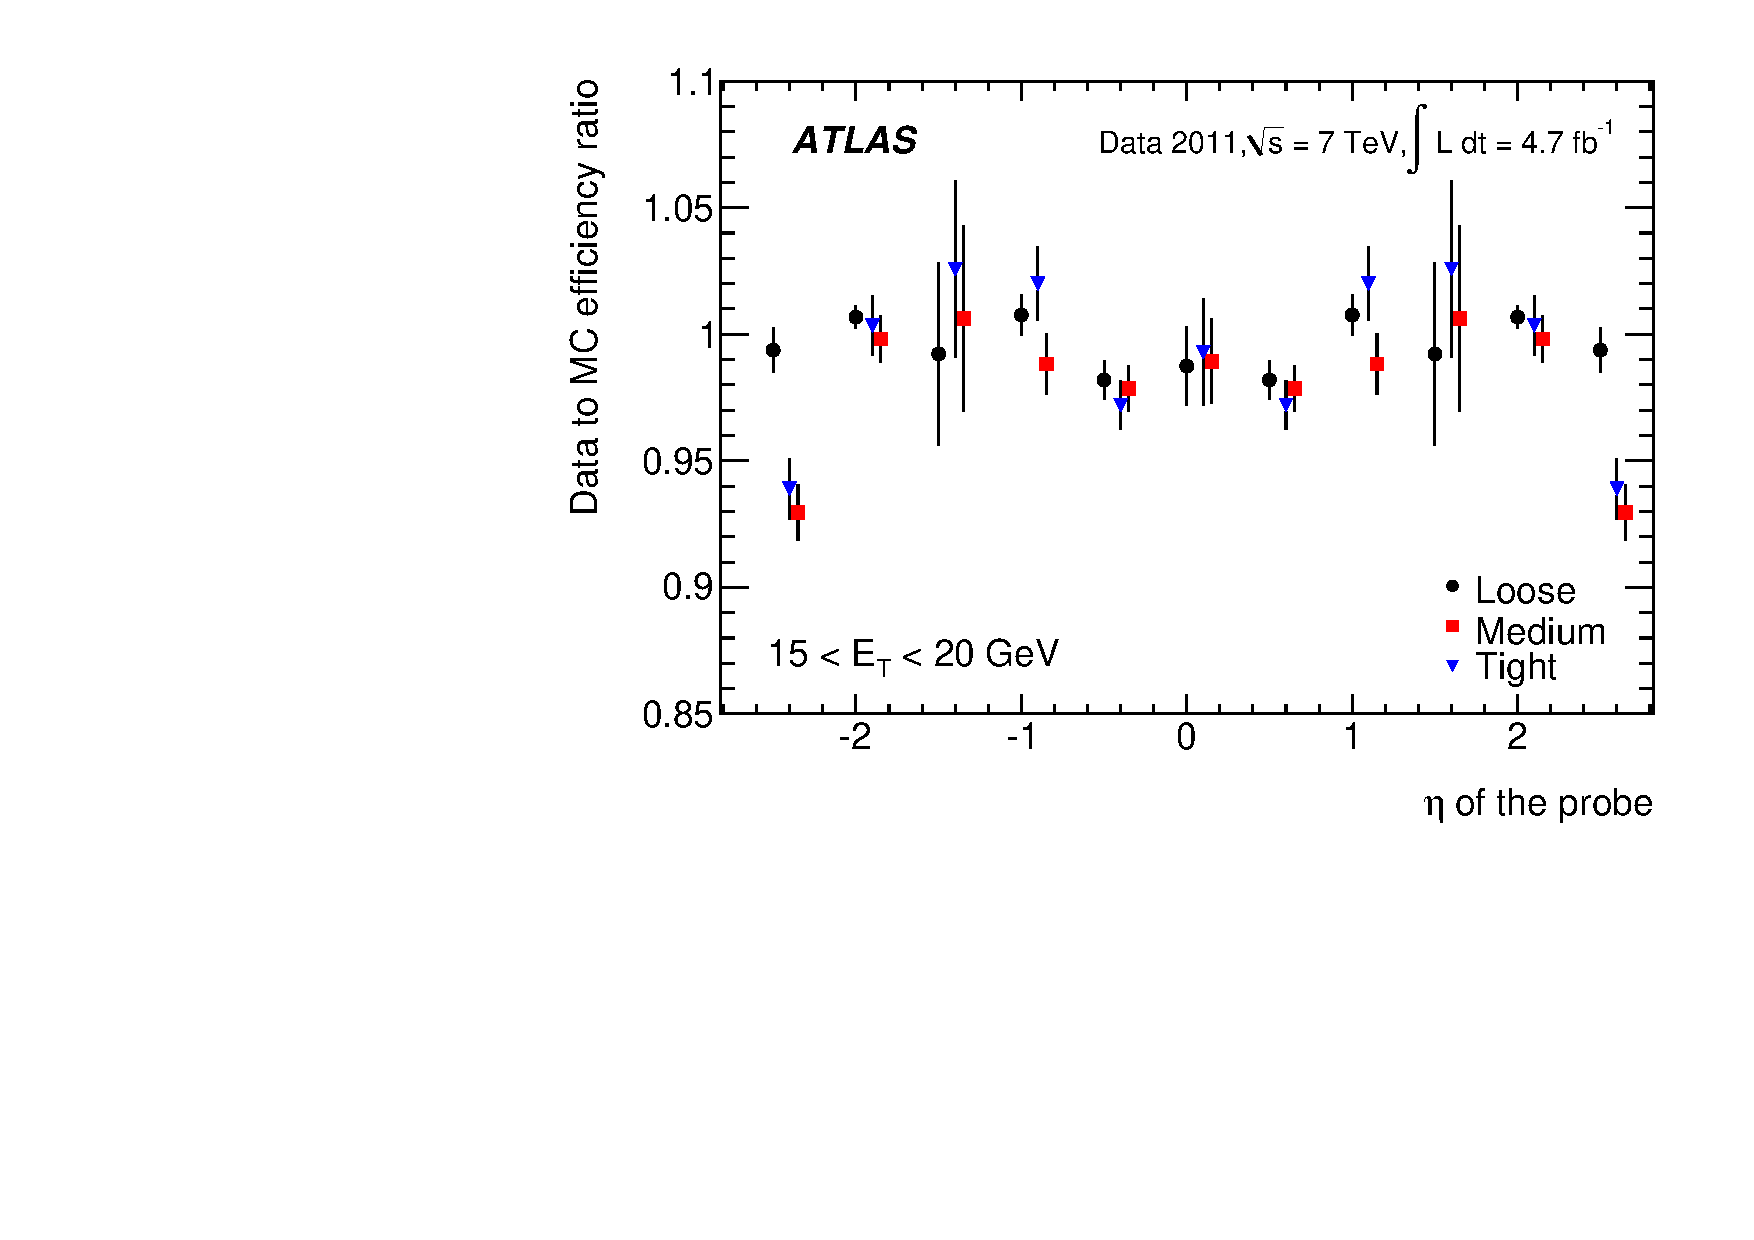
\includegraphics[width=0.45\textwidth]{figures/eff_rec_id_SFs_a.pdf}}
\subfigure[$35 < \et < 40$]{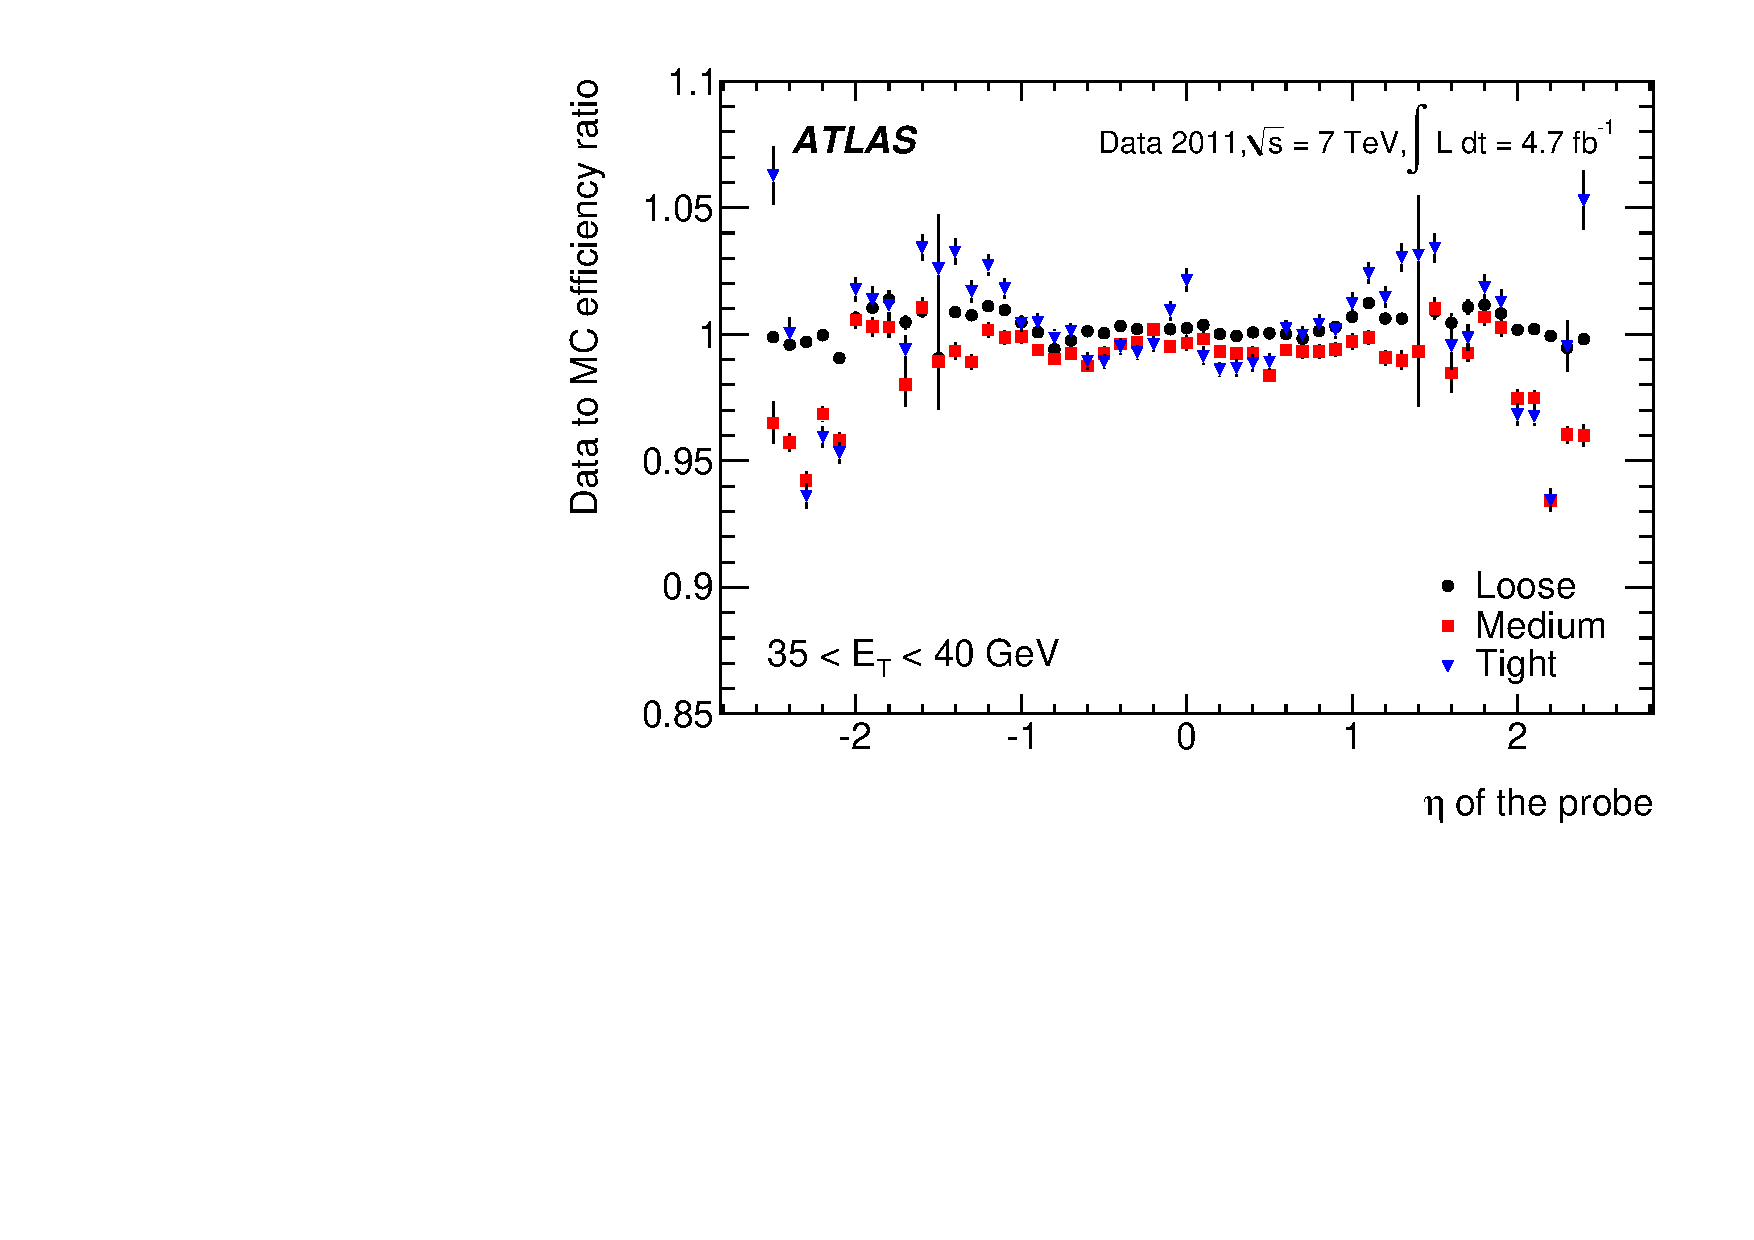
\includegraphics[width=0.45\textwidth]{figures/eff_rec_id_SFs_b.pdf}}

\caption[Examples of combined scale factors for the three identification criteria (loose, medium, tight) as a function of the pseudorapidity of the probe-electron $\eta$. Results are shown for different ranges of the probe electron energy. The error bars indicate the total uncertainties.]{Examples of combined scale factors for the three identification criteria (loose, medium, tight) as a function of the pseudorapidity of the probe-electron $\eta$. Results are shown for different ranges of the probe electron energy. The error bars indicate the total uncertainties.~\cite{lib:elec_reco}}
\label{fig:eff_rec_id_SFs}}
\end{figure}

\subsection{Forward electron identification efficiencies}

In the forward region of the calorimeters, the electron identification efficiency is measured with a \Zee\ central-forward sample  where  a  well-isolated $\et > 25$~GeV tag  electron satisfying the tight requirement is identified in the central region of the calorimeter and the probe cluster with $\et > 20$~GeV is found in the forward region. As an additional cut the low $\et^{miss}$ is required for the event candidates to suppress the contributions from \Wenu\ events.
The invariant mass $m_{ee}$ is fitted by the Crystal Ball function convoluted with a non-relativistic Breit-Wigner function with fixed $Z$ width to model the signal, and a Landau function to model the background in a mass window of $55 < m_{ee} < 130$~GeV. The S/B ratio is $\sim$7 for the outer EMEC and $\sim$5 for the FCAL. The various shifts to the tag requirements and to the fit parameters were performed to determine the amount of the systematical uncertainties, the resulting scale factors for selected bins can be seen in Figure~\ref{fig:eff_rec_id_forward_SFs}.

\begin{figure}
\center{
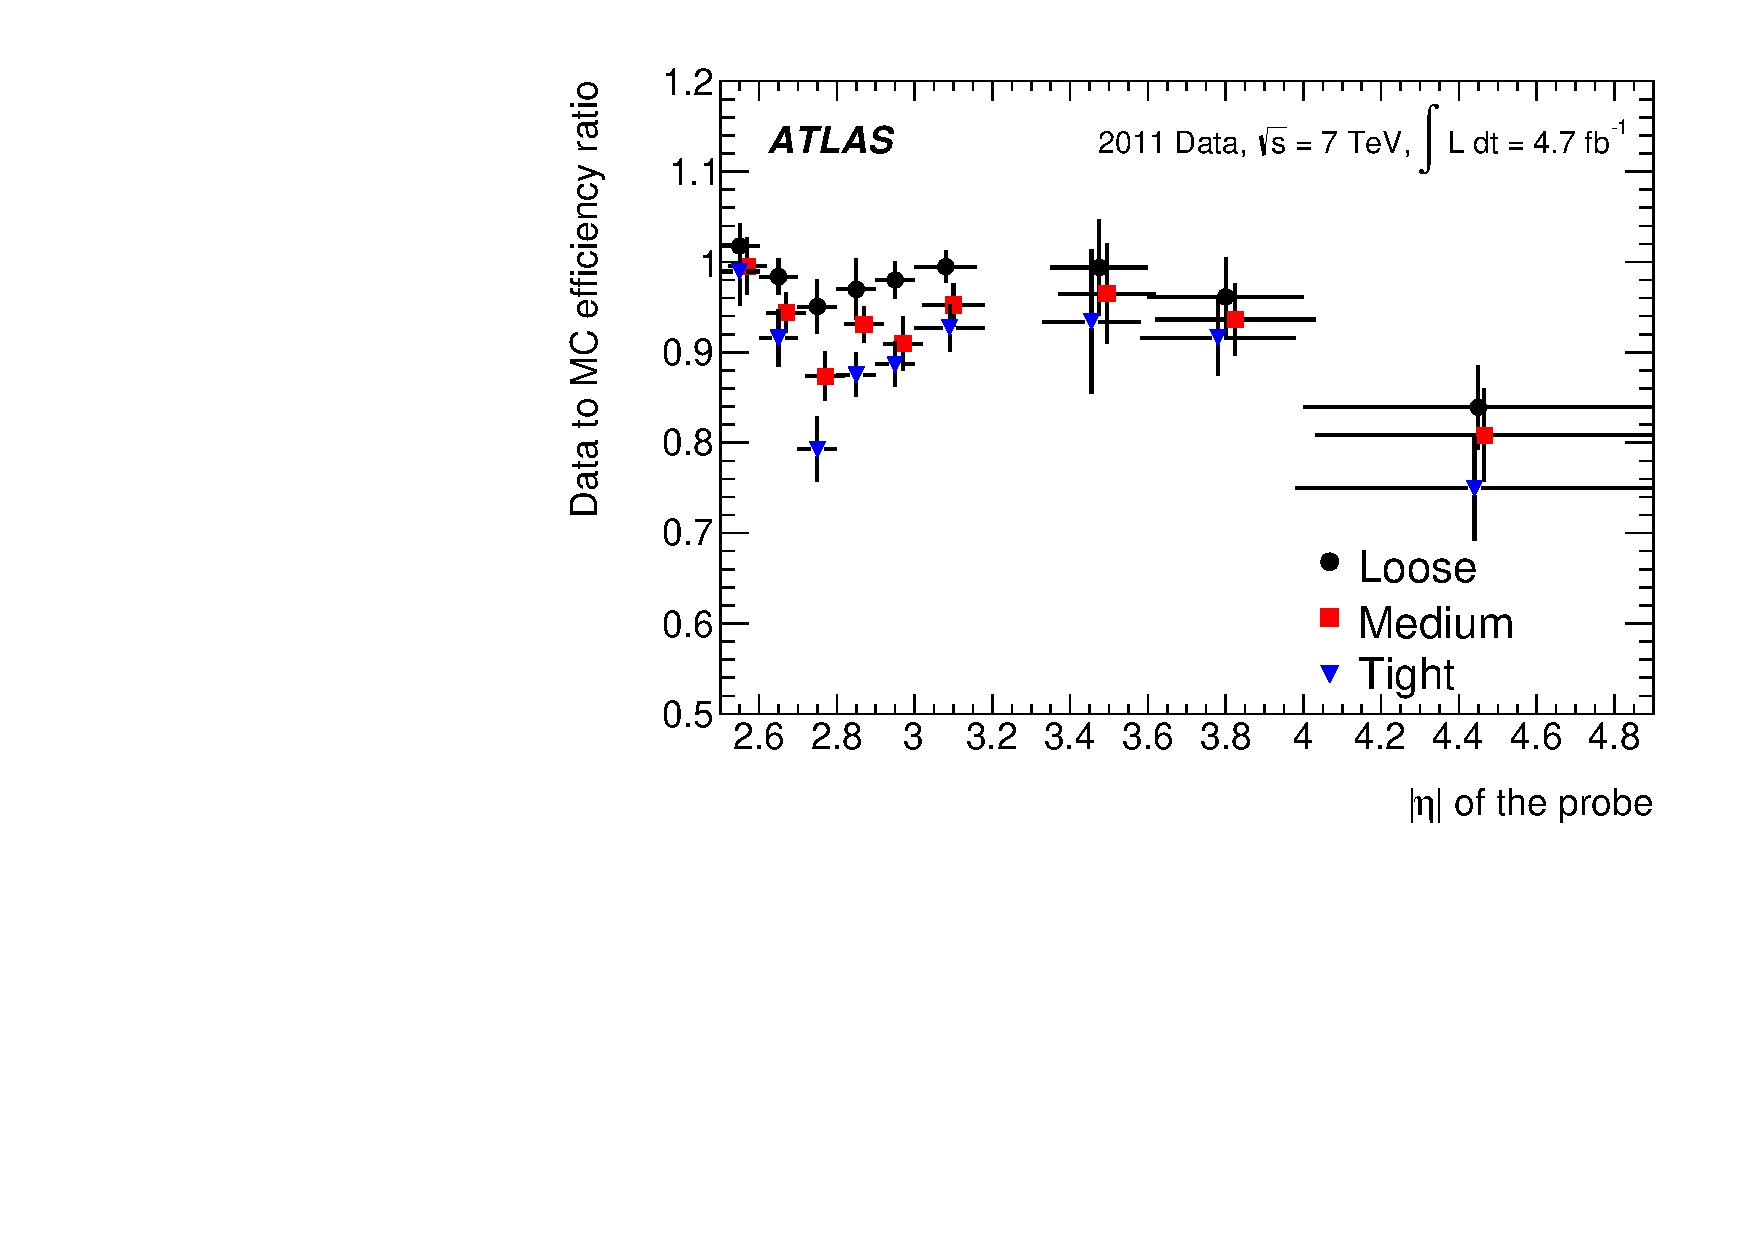
\includegraphics[width=0.5\textwidth]{figures/eff_rec_id_forward_SFs.pdf}
\caption[The scale factors for the forward electrons with $\et > 20$~GeV. The error bars correspond to the total uncertainties.]{The scale factors for the forward electrons with $\et > 20$~GeV. The error bars correspond to the total uncertainties.~\cite{lib:elec_reco}}
\label{fig:eff_rec_id_forward_SFs}}
\end{figure}


\subsection{Reconstruction efficiencies}

For reconstruction efficiency measurements the events from the \Zee\ channel are used for both central and forward electrons. As discussed in Section~\ref{sec:Rec_elec} the algorithm for the forward electrons is much more complex and gives an efficiency of about 97\% at 7~GeV and $\sim$99\% at 15~GeV. For the higher energies the efficiency of it is matched by that of the track reconstruction and cluster-track matching algorithms.

Efficiency values were measured for three samples:

\begin{itemize}
\item All reconstructed electron candidates in \Zee\ channel;
\item All the same electron candidates, but with additional requirement of the quality of the matching track, to match with the $J/\psi \to ee$ conditions described above;
\item All reconstructed electron candidates with additional requirements on hadronic leakage and the track quality to match with the \Wenu\ conditions described above.
\end{itemize}

The conditions for these measures follows that of the identification closely, except for the corrections for the photon conversions: the photons are included in the denominator when calculating the efficiency, provided they satisfy all the requirements. Naturally, that also means that the opposite sign requirement also doesn't apply.

For the background evaluation the same technique is applied: the background template is constructed using the inversion of several ID cuts (at least two from the loose ID not counting the ones dealing with the track) and failing the isolation requirement, and then normalized to the data in the high-mass region ($110 < m_{ee} < 250$~GeV).

The three samples together with the variations obtained from the variations of the background thresholds are used to find the systematic uncertainties with the same method as used in the identification efficiency calculation.

The resulting efficiencies can be seen in Figure~\ref{fig:eff_rec}. It can be seen that the systematical error increases greatly at $\et < 20$~GeV.

\begin{figure}
\center{
\subfigure[Reconstruction efficiencies]{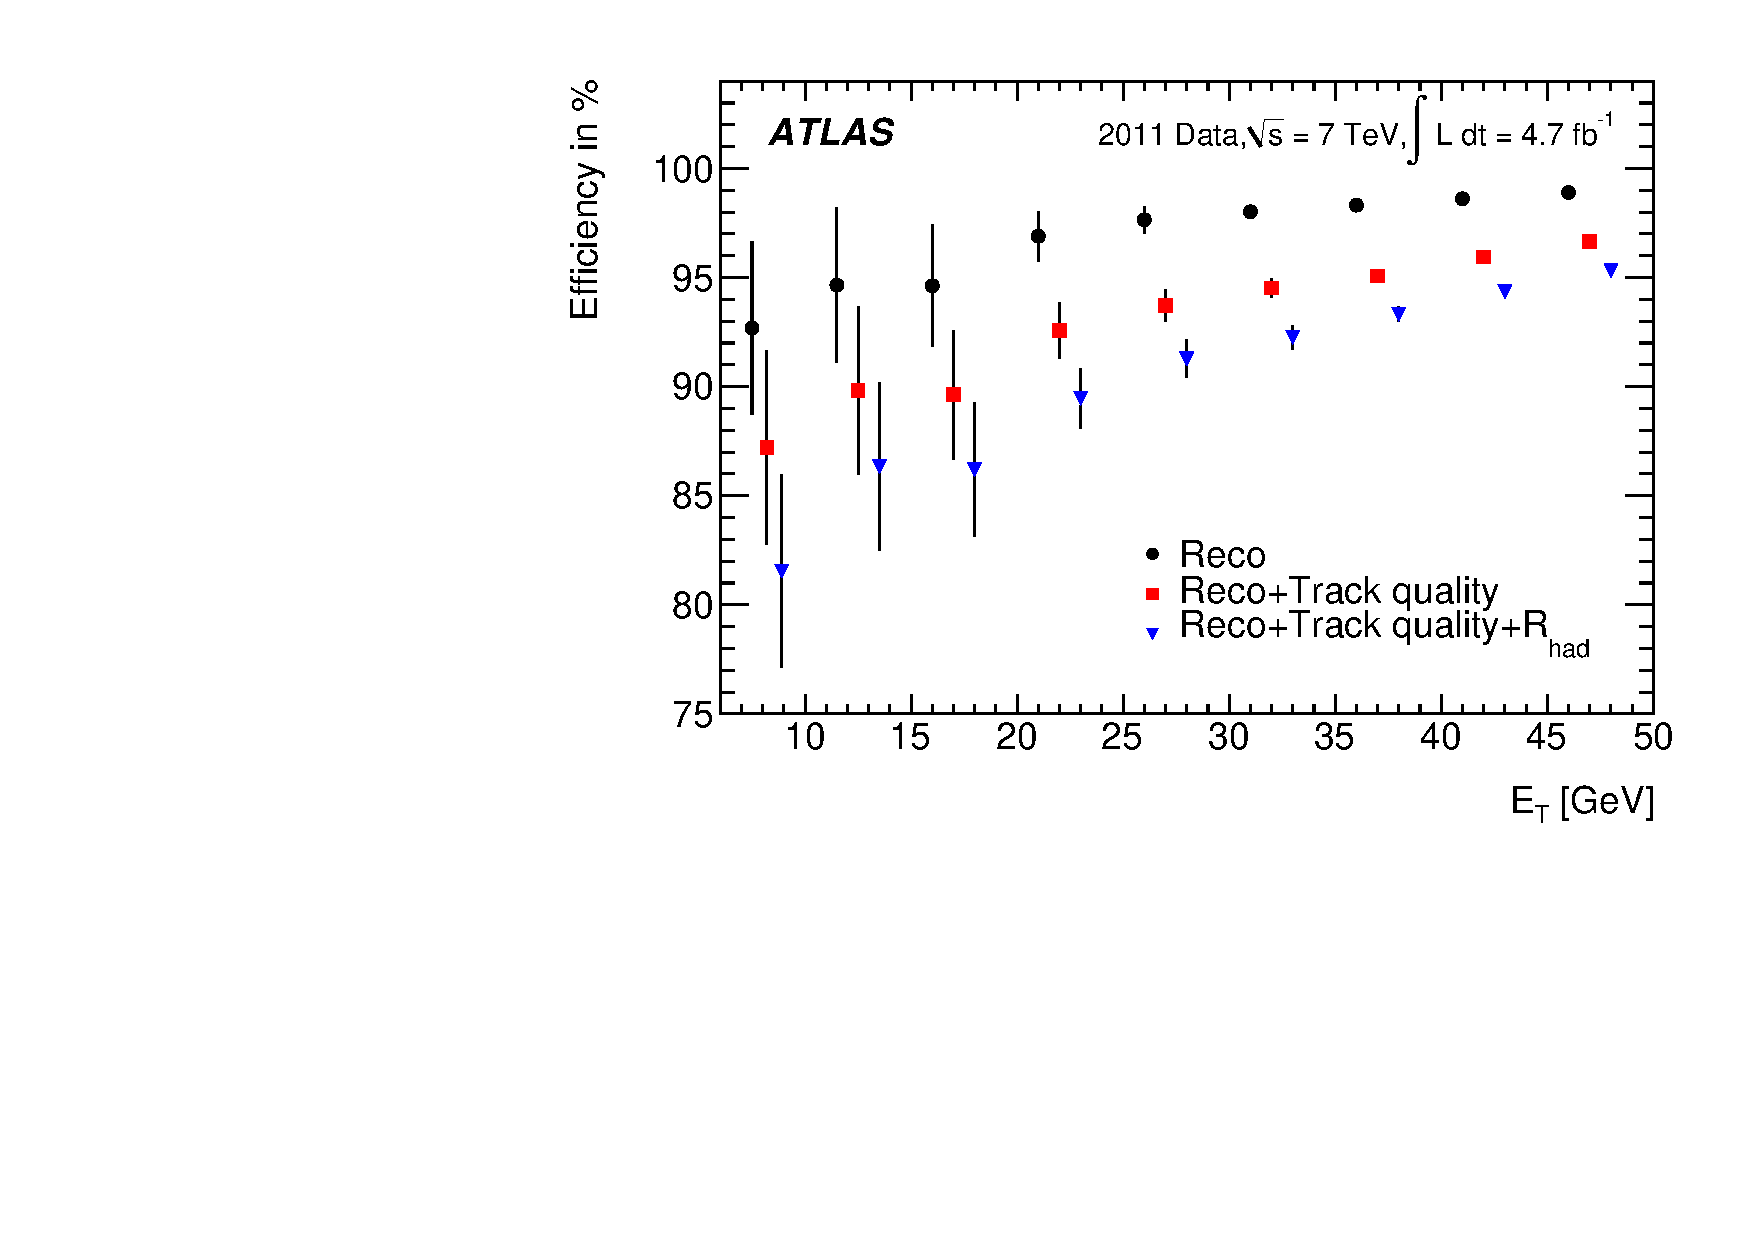
\includegraphics[width=0.45\textwidth]{figures/eff_rec_a.pdf}}
\subfigure[Systematical and statistical uncertainties]{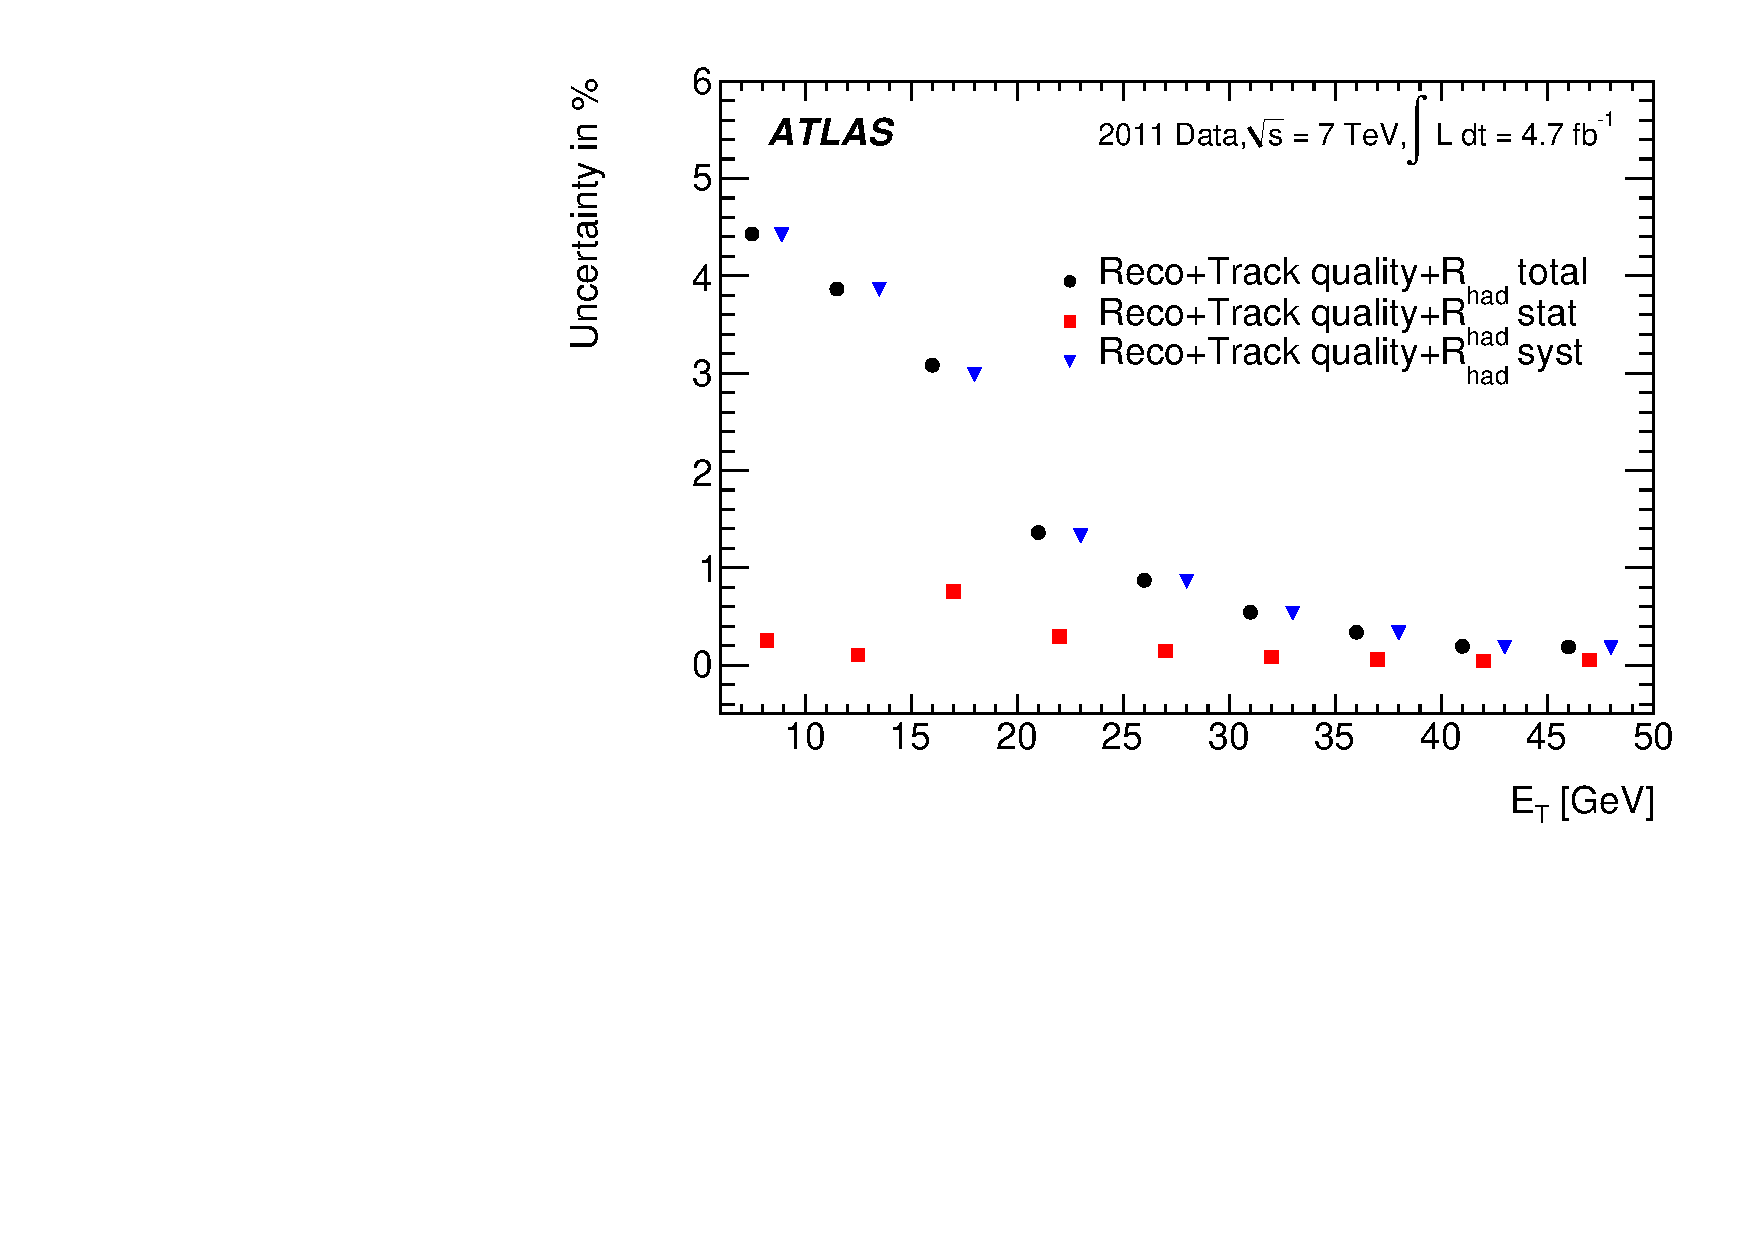
\includegraphics[width=0.45\textwidth]{figures/eff_rec_b.pdf}}

\caption[Reconstruction efficiencies for the central electrons, the error bars represent the total uncertainty, which can be seen fully in (b).]{Reconstruction efficiencies for the central electrons, the error bars represent the total uncertainty, which can be seen fully in (b).~\cite{lib:elec_reco}}
\label{fig:eff_rec}}
\end{figure}

\section{Isolation efficiency}

In the central-forward event selection of \Zee\ analysis the two additional isolation cuts are used in order to reduce the amount of the background: Iso98\et$^{\mathrm{cone20}}$ and Iso97\pt$^{\mathrm{cone40}}$ one being for the track and the other for the cluster. The efficiency of the isolation is thus the fraction of the electrons that pass this additional cut:
\begin{equation}
\varepsilon_\mathrm{Iso} = \frac{N_\text{probe with Iso} }{ N_\text{all probe} }, \;\;\;\;
\delta \varepsilon_\mathrm{Iso} = \frac{\sqrt{(1-2\varepsilon) \delta N_\text{probe with Iso}^2 + \varepsilon^2 \delta N_\text{all probe}^2}}
                                {N_\text{all probe}},
\end{equation}
where $\varepsilon_\mathrm{Iso}$ is the efficiency, and $\delta \varepsilon_\mathrm{Iso}$ is the corresponding statistical error.

The measurement was done with the \Zee\ sample with the same setup, with the \pt\ cut of the probe electron being lowered to 15~GeV and mass window reduced to $80 < m_{ee} < 100$~GeV to remedy the increased background. The remaining background is negligible (less than $0.1$\%).

The systematical error evaluation was done by shifting the mass window in the same way as the calculation of the trigger efficiencies, and by increasing the \pt\ cut for the tag electron to 24~GeV. The resulting efficiencies can be seen in Figure~\ref{fig:eff_iso_SFs}.

\begin{figure}
\center{
\subfigure[Isolation scale factors]{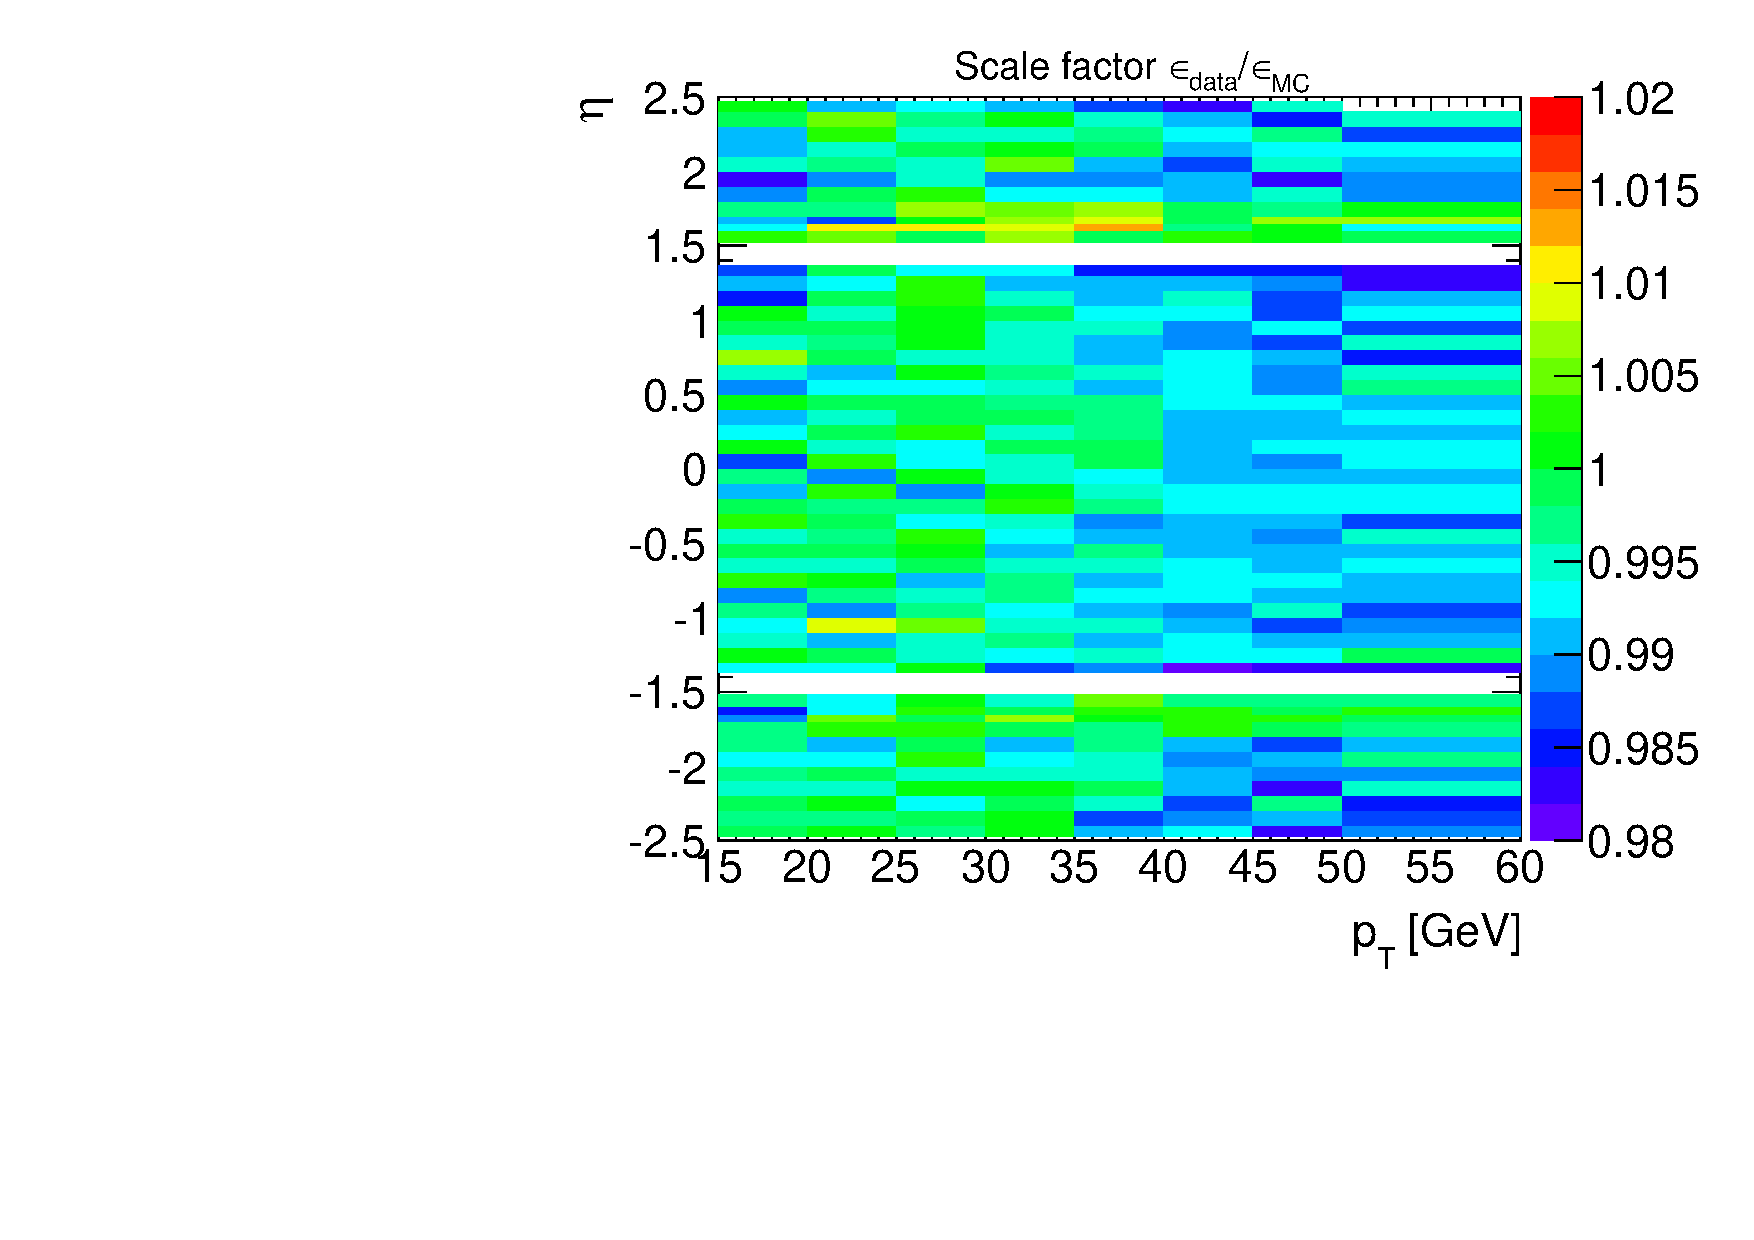
\includegraphics[width=0.45\textwidth]{figures/eff_iso_SFs.pdf}}
\subfigure[Statistical uncertainties]{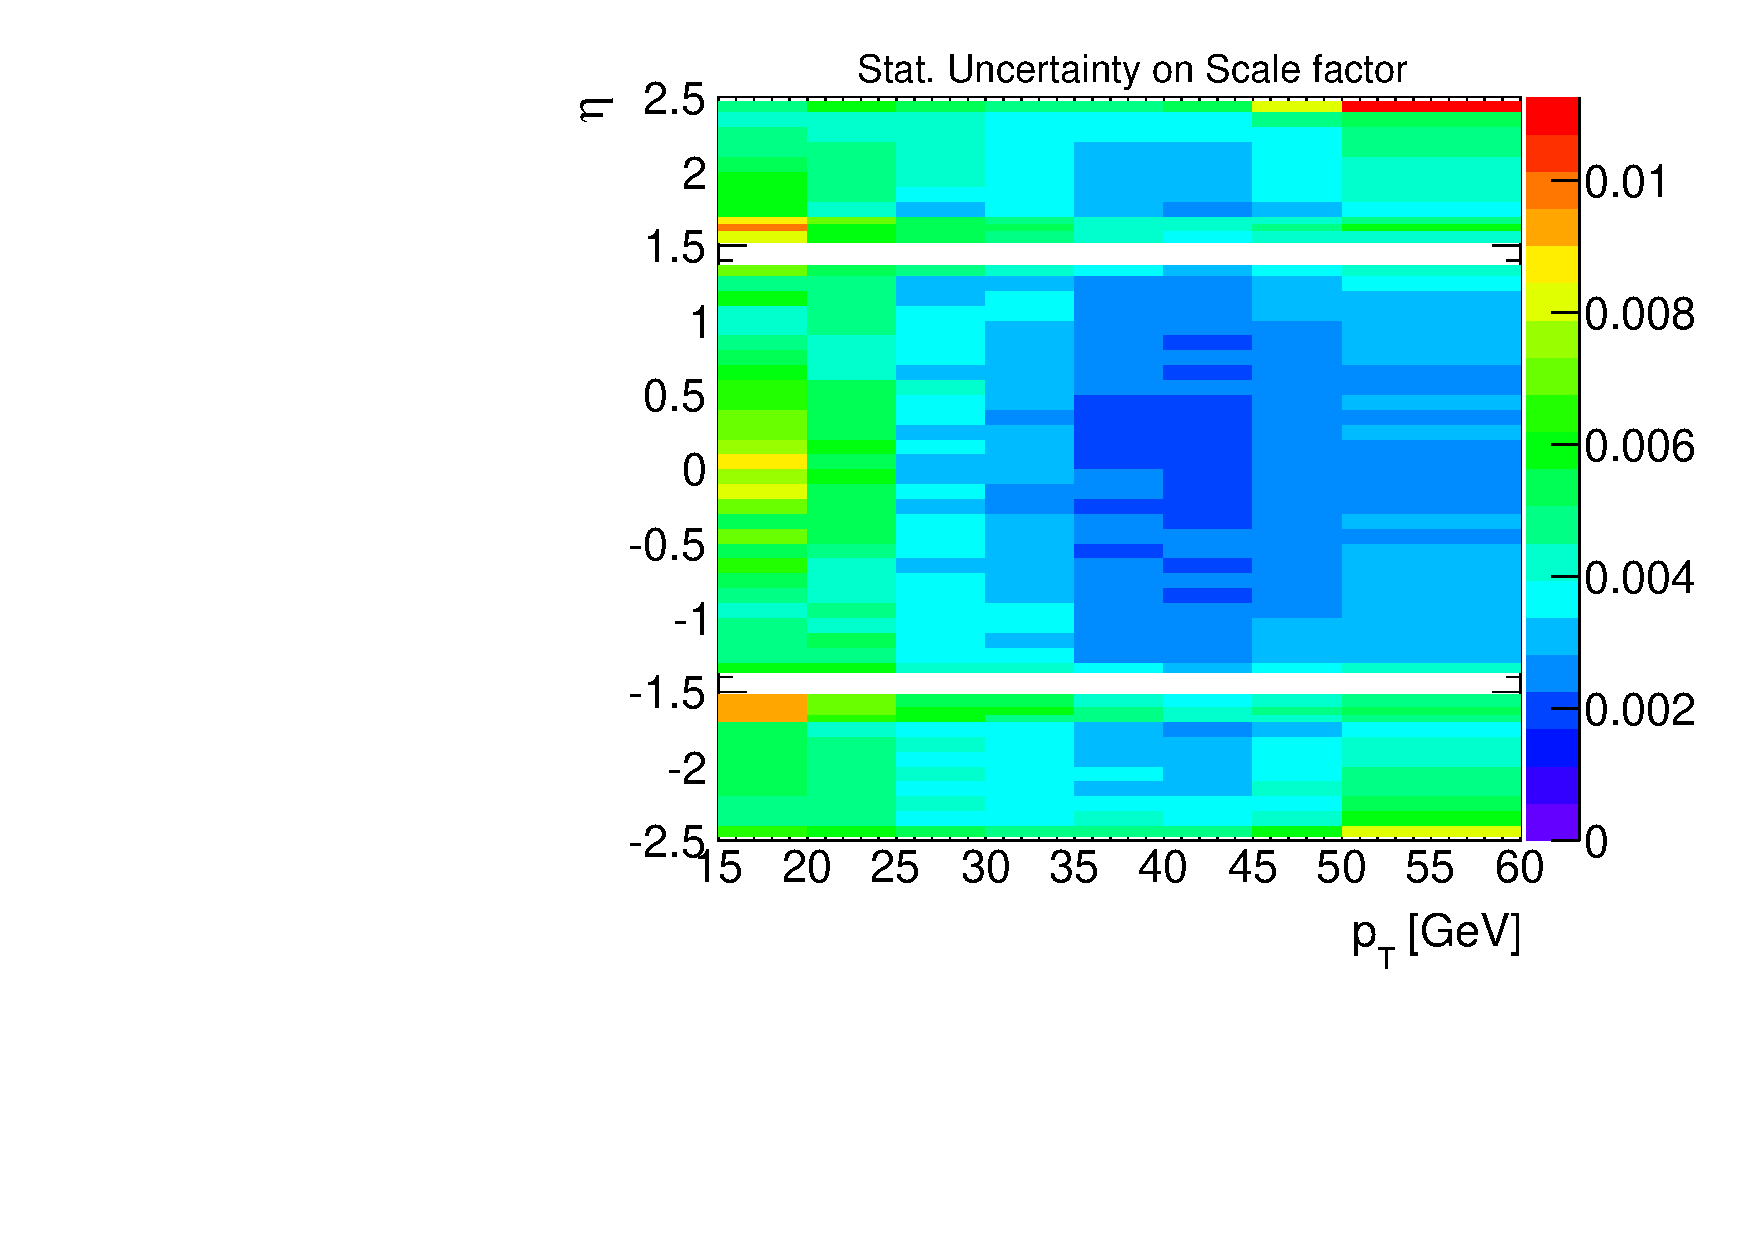
\includegraphics[width=0.45\textwidth]{figures/eff_iso_unc.pdf}}

\caption{Scale factors for the isolation efficiencies for the 2011 data together with statistical uncertainties in 2D binning by \pt\ and $\eta$. The plots were made using the \Zee\ MC samples with standard CC analysis cuts with the additional requirements on electron ID from the CF analysis.}
\label{fig:eff_iso_SFs}}
\end{figure}

\chapter{Background estimation}
\label{sec:Bkg}

As was described in Sec.~\ref{sec:Selection}, the selection phase is designed to suppress the background events (i.e. not \Zee\ events) while keeping the signal events. But even with all the cuts applied, some of the background events still pass all of them. In order to get the correct results, we need to estimate the number of the background events in our selection.

The background events come in two flavours: the electroweak (EW) background and the QCD background. The difference from the analysis point of view is in that we can directly predict the amount of the EW background based on the MC simulation (except for two components which will be discussed later), while the QCD background we have to estimate, using so-called fits based on the indirect data. Both of these methods will be descrabed here.

\section{Electroweak background}

The sources of the electroweak background are the events that came from various electroweak decays but were misinterpreted as \Zee. The list of the processes that contribute to the EW background was given in Tab.~\ref{tab:MC_bg}. There are eight of them, including three single-boson decays, three di-boson decays, \ttbar, and photon induced background. All the processes except the last one have a cross-section comparable with \Zee\ which can be reliably predicted by the theory, and also use the same effiviency coefficients as signal, and therefore can be simulated using MC. For the photon-induced background the situation is more complicated. We can't reliably evaluate the amount of this background, and the relative uncertainty for it is usually 30-50\%. This background is added after the unfolding.

The electroweak background is largely dominated by the \Wenu\ events, where the electron goes to the central part of the calorimeter, and the fake forward electron is produced by the W+jet activity. Since the jet behaviour in the forward region is modelled poorly, this background is normalized to data, instead of theoretical-driven luminocity normalization used for other backgrounds.

For the \Wenu\ evaluation three selections were used, all of them in two mass windows around mass peak: $66 < m_{ee} < 80$~GeV and $100 < m_{ee} < 150$~GeV, but two of them also have an additional cuts:
\begin{itemize}
\item $E_{t}^{miss} > 25$~GeV;
\item $E_{t}^{miss} > 25$~GeV, $M_{t} > 50$~GeV.
\end{itemize}
These three selections were used to normalize the \Wenu\ background in high bins of $E_{t}^{miss} > 70$~GeV. Since both this and QCD backgrounds use the same method of fitting to data, they interfere with each-other. But since the fitting is done in different parts of the phase space, they correlate very little with each-other, and so only one additional iteration is required to obtain valid results. The fitted background can be seen in Fig.~\ref{fig:bkg_wenu}.

\begin{figure}
\center{
\subfigure[Mass window] {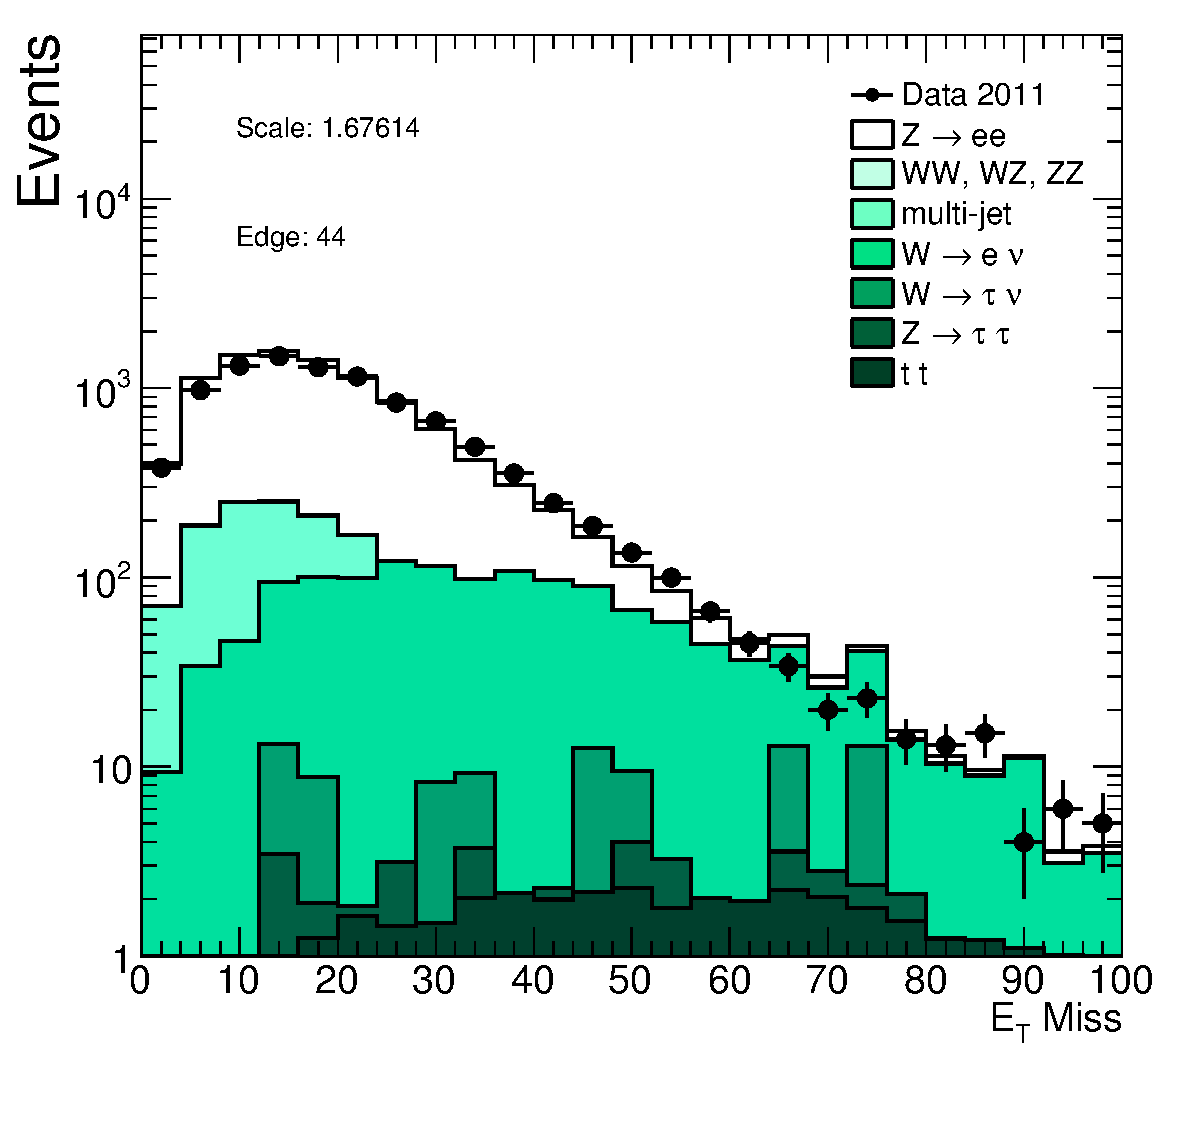
\includegraphics[width=0.32\textwidth]{figures/bkg_wenu_1.pdf}}
\subfigure[Mass window, $E_{t}^{miss}$]  {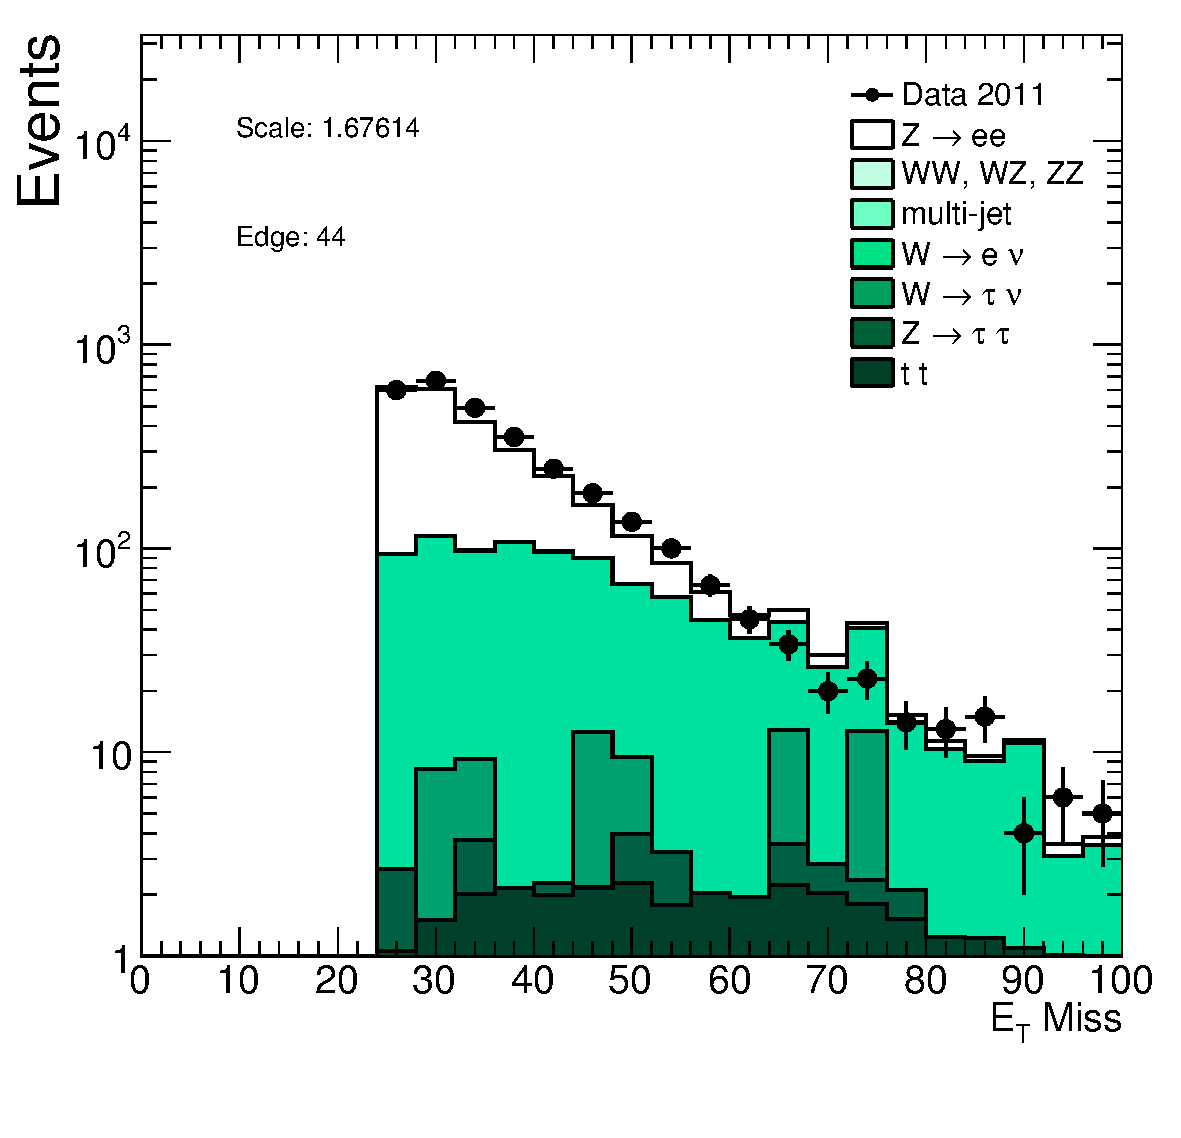
\includegraphics[width=0.32\textwidth]{figures/bkg_wenu_2.pdf}}
\subfigure[Mass window, $E_{t}^{miss}$, $M_{t}$] {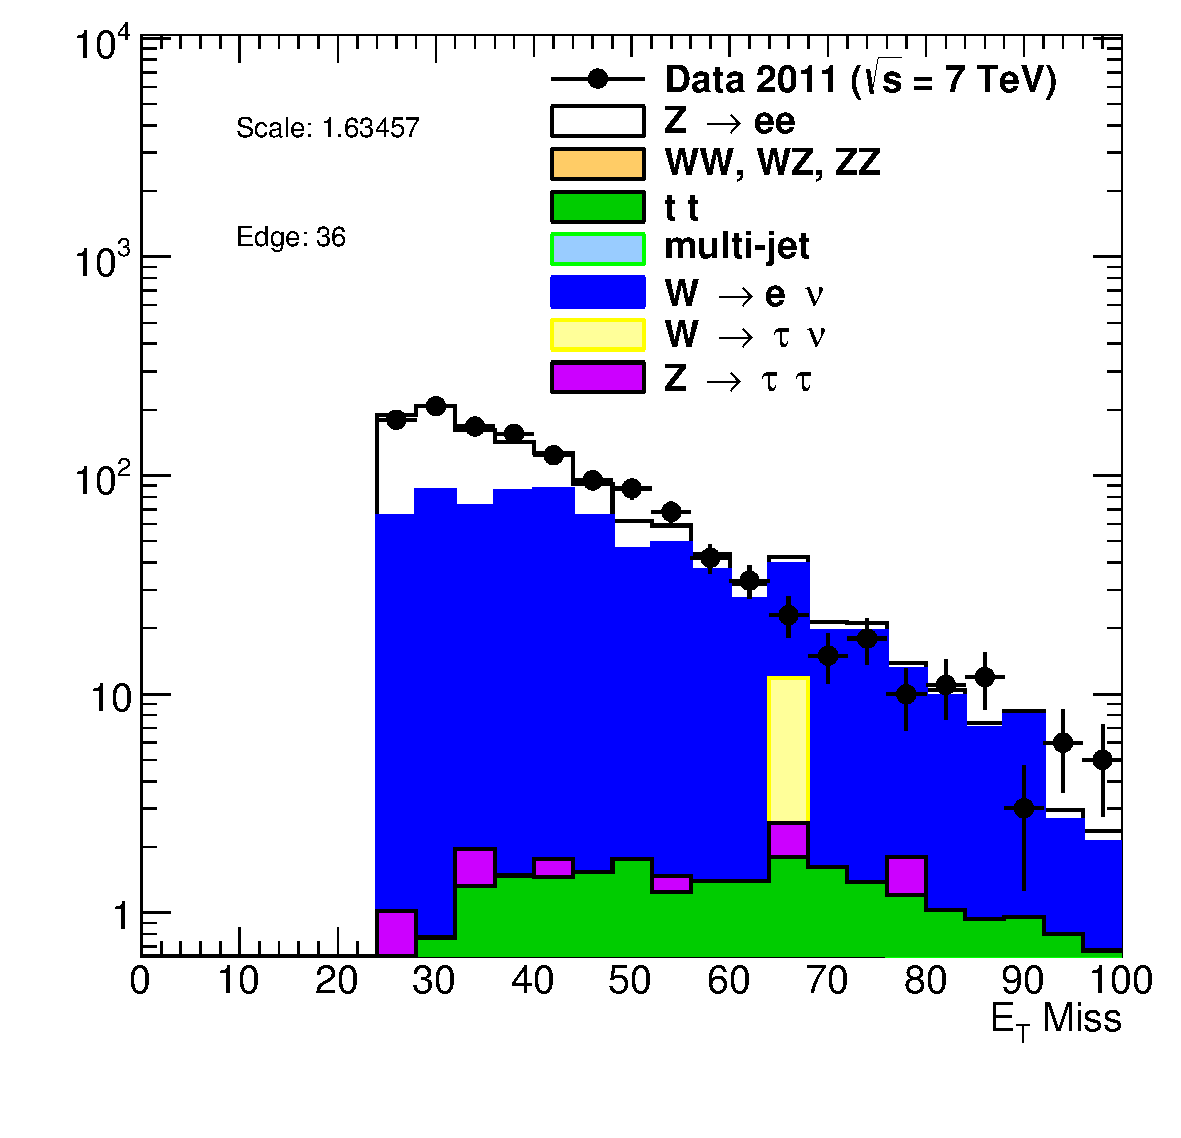
\includegraphics[width=0.32\textwidth]{figures/bkg_wenu_3.pdf}}

\caption{The data-fitting of the \Wenu\ background with various selections. (a) Mass window selection, (b) Mass window and $E_{t}^{miss} > 25$~GeV, (c) Mass window, $E_{t}^{miss} > 25$~GeV and $M_{t} > 50$~GeV.}
\label{fig:bkg_wenu}}
\end{figure}

All other electroweak backgrounds are simply scaled to the theoretically predicted luminocity-derived values. The resulting values for the electroweak background can be seen in Tab.~\ref{tab:bkg_ew_peak} for the peak mass, and in Tab.~\ref{tab:bkg_ew_high} for the high mass.

\begin{table}
\centering
\begin{tabular}{ c cccccccc } \hline \hline
 $y_Z$ bin & $t\bar t$ & $W \to e\nu$ & $W \to \tau\nu$ &  $WW$ & $WZ$ & $ZZ$ & $Z \to \tau\tau$  & $\gamma\gamma \to ee$\\  \hline
 1.2 -  1.4 &   0.18 &   1.90 &   0.00 &   0.04 &   0.08 &   0.04 &   0.01 &   0.10 \\
 1.4 -  1.6 &   0.11 &   1.61 &   0.38 &   0.03 &   0.07 &   0.03 &   0.06 &   0.09 \\
 1.6 -  1.8 &   0.08 &   1.10 &   0.10 &   0.03 &   0.05 &   0.03 &   0.09 &   0.08 \\
 1.8 -  2.0 &   0.06 &   1.03 &   0.00 &   0.02 &   0.04 &   0.02 &   0.06 &   0.07 \\
 2.0 -  2.2 &   0.04 &   0.87 &   0.03 &   0.02 &   0.04 &   0.02 &   0.08 &   0.05 \\
 2.2 -  2.4 &   0.03 &   0.75 &   0.10 &   0.02 &   0.04 &   0.02 &   0.10 &   0.05 \\
 2.4 -  2.8 &   0.01 &   0.65 &   0.13 &   0.02 &   0.04 &   0.02 &   0.11 &   0.05 \\
 2.8 -  3.2 &   0.00 &   0.35 &   0.08 &   0.01 &   0.02 &   0.01 &   0.08 &   0.04 \\
 3.2 -  3.6 &   0.00 &   0.05 &   0.00 &   0.00 &   0.01 &   0.01 &   0.01 &   0.03 \\
\hline \hline
\end{tabular}
\caption{Components of the electroweak background  in \% of selected data for $66 < m_{ee} < 116$~GeV.}
\label{tab:bkg_ew_peak}
\end{table}

\begin{table}
\centering
\begin{tabular}{ c cccccccc } \hline \hline
 $y_Z$ bin & $t\bar t$ & $W \to e\nu$ & $W \to \tau\nu$ &  $WW$ & $WZ$ & $ZZ$ & $Z \to \tau\tau$  & $\gamma\gamma \to ee$\\  \hline
 1.2 -  1.6 &   2.17 &  22.40 &   0.00 &   0.64 &   0.30 &   0.04 &   0.61 &   0.98 \\
 1.6 -  2.0 &   1.22 &  17.06 &   1.70 &   0.64 &   0.22 &   0.04 &   0.52 &   0.98 \\
 2.0 -  2.4 &   0.62 &   9.98 &   1.30 &   0.39 &   0.15 &   0.03 &   0.19 &   0.67 \\
 2.4 -  2.8 &   0.21 &   8.12 &   0.00 &   0.24 &   0.10 &   0.03 &   0.25 &   0.52 \\
 2.8 -  3.2 &   0.07 &   3.14 &   0.00 &   0.14 &   0.07 &   0.01 &   0.00 &   0.53 \\
 3.2 -  3.6 &   0.00 &   0.00 &   0.00 &   0.00 &   0.03 &   0.00 &   0.00 &   0.29 \\
\hline \hline
\end{tabular}
\caption{Components of the electroweak background in \% of selected data for $116 < m_{ee} < 150$~GeV.}
\label{tab:bkg_ew_high}
\end{table}

\section{QCD background}

The QCD background is the name for the multi-jet hadronic background. Since it's nearly impossible to simulate all the multitude of the hadronic processes with even remote accuracy. There are two methods to evaluate the amount of the multi-jet background. The first one is by using the theoretical functions to evaluate the form of the background. Usually the convolution of the Crystal Ball and the Breit-Wigner functions is used with the use of the RooFit framework~\cite{lib:bkg_roofit}. The second method is more precise and is usually used when the data samples are large enough to provide the adequate statistical error, and consist of constructing the background template (i.e. the form) from the data itself, by using the cut inversion: several cuts in the selection chain (usually the most basic ones) are inverted to provide the sample of the background events with the most "signal-like" signature. The amount of such events is usually very limited, but the total amount of the 2011 data allows us to use this method, which is otherwise better than the theoretical predictions of the RooFit method.

In both cases, after the template is constructed, it is normalized to the data, which is done by using the discriminatory variable. This variable shows how much background there is in any particular bin, to distinguish background-dominated bins from the signal-dominated bins. For the \Zee\ CF analysis the discriminatory variable was the isolation of the central electrone cluster $E_{t}^{\mathrm{cone30}}$. This variable showed the best results among the other tested, but since it is used in the default analysis selection, it can't be used direclty, and the background was normalized to the selection without the isolation cuts, and then scaled accordingly.

The background template is constructed based on the three selections: the one with the default cuts, with the default cuts and relaxed track and cluster isolation, and with the default cuts and relaxed cluster isolation only. For all selection the cut inversion included some of the electron tight ID criteria. See Tab.~\ref{tab:bkg_qcd_samples}. To calculate the systematic uncertainties for the background additional selections must be constructed. These selections must take into account the way the background is scaled: it is matched to the data in high-$E_{t}^{\mathrm{cone30}}$ bin, and the isolation cuts are not applied. See Tab.~\ref{tab:bkg_qcd_unc_samples} for the list.

\begin{table}
\centering
\begin{tabular}{ llll } \hline \hline
    & Cut inversion  &   Base selection    & expected bkg  \\ \hline
default & FwdTight, Tight++ & Default  & isolated \\
$S_1$   & FwdTight, Tight++ & Default w/o calo and track iso & all \\
$S_2$   & FwdTight, Tight++ & Default w/o calo iso       & $P_{t}^{\mathrm{cone}}$ isolated\\
\hline \hline
\end{tabular}
\caption{Event selections for QCD background estimation.}
\label{tab:bkg_qcd_samples}
\end{table}
\begin{table}
\centering
\begin{tabular}{ lll@{ w/o }ll } \hline \hline
    & Cut inversion  &  \multicolumn{2}{l}{Base selection}    & expected bkg \\ \hline
default\_1 & Tight++     & Default & FwdTight  & isolated \\
$S_2$\_1     & Tight++     & $S_1$ & FwdTight      & all \\
default\_2 & FwdMedium++ & Default & Tight++   & isolated \\
$S_2$\_2     & FwdMedium++ & $S_1$ & Tight++       & all \\
\hline \hline
\end{tabular}
\caption{Event selections for QCD background systematic uncertainties calculation.}
\label{tab:bkg_qcd_unc_samples}
\end{table}

The normalization procedure was made in several iterations, during which the background template and the signal MCs were scaled together to fit the data best, until the MC signal scalefactor is stabilized. Step by step explanation of the procedure is this:
\begin{itemize}
\item template is scaled to data based on the isolation tail bins: $s_{\mathrm{temp}} = \frac{N_{\mathrm{data}}^{\mathrm{tail}} - (s_{\mathrm{sig}} \cdot N_{\mathrm{sig.MC}}^{\mathrm{tail}}+N_{\mathrm{EWbkg}}^{\mathrm{tail}})}{N_{\mathrm{temp}}^{\mathrm{tail}}}$, where
\begin{itemize}
\item $s_{\mathrm{temp}}$ is the scalefactor for the QCD template;
\item $s_{\mathrm{sig}}$ is the scalefactor for the signal MC, which is $1.0$ at the first step;
\item $N_{\mathrm{data}}^{\mathrm{tail}}$ is the data events integrated over the isolation tail bins;
\item $N_{\mathrm{sig.MC}}^{\mathrm{tail}}$ is the signal MC events integrated over the isolation tail bins;
\item $N_{\mathrm{EWbkg}}^{\mathrm{tail}}$ is the electroweak background MC events integrated over the isolation tail bins;
\item $N_{\mathrm{temp}}^{\mathrm{tail}}$ is the template events integrated over the isolation tail bins;
\end{itemize}
\item the scaled template (i.e. the QCD background) is substracted from the data togethe with the electroweak background, and the remaining events are compared to signal MC to determine the new scalefactor for the MC: $s_{\mathrm{sig}} = \frac{N_{\mathrm{data}} - (s_{\mathrm{temp}} \cdot N_{\mathrm{temp}} + N_{\mathrm{EWbkg}})}{N_{\mathrm{sig.MC}}}$, where all the variables are the same, only integrated over all bins, not only the tail bins;
\item if the new MC scalefactor differs from the previous by less then $0.1$\%, the template scalefactor is considered to be final, otherwise, the new iteration is made.
\end{itemize}

For the systematic uncertainties, several values were used as the threshold of the tail region. For the central values, the template $S_{1}$ with $E_{t}^{\mathrm{cone30}}$ was chosen, as the one with the clearer separation of the background-dominated bins, and the most stable fit. The resulting QCD background estimations can be seen in Figs.~\ref{fig:bkg_qcd} and in Tabs.~\ref{tab:bkg_qcd_peak_percents} and~\ref{tab:bkg_qcd_high_percents}.

\begin{figure}
\center{
\subfigure[$66 < m_{ee} < 116$~GeV] {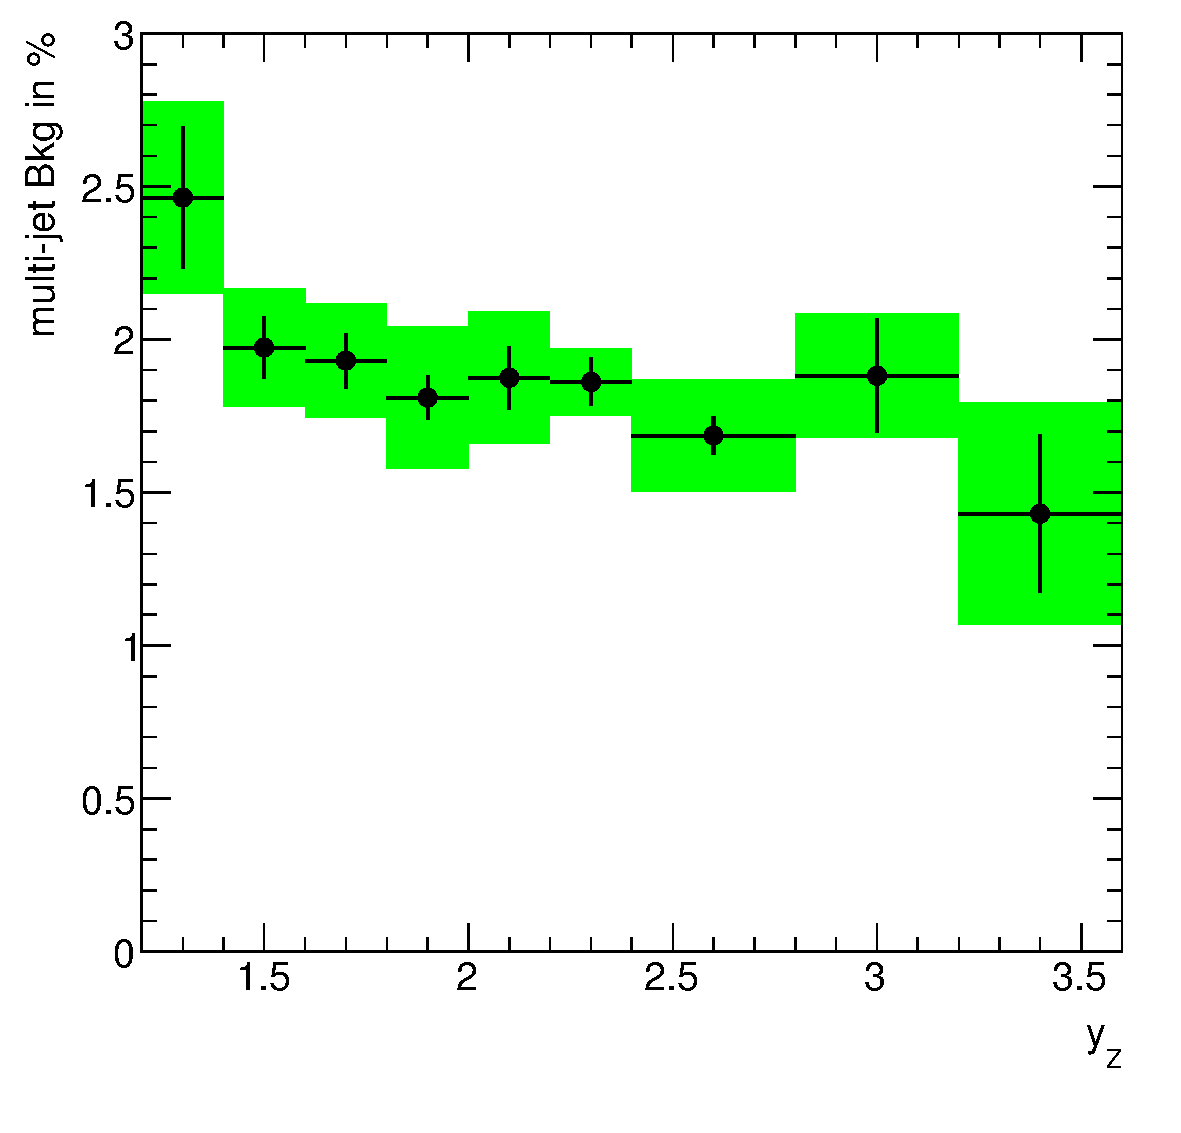
\includegraphics[width=0.45\textwidth]{figures/bkg_qcd_peak.pdf}}
\subfigure[$116 < m_{ee} < 150$~GeV]  {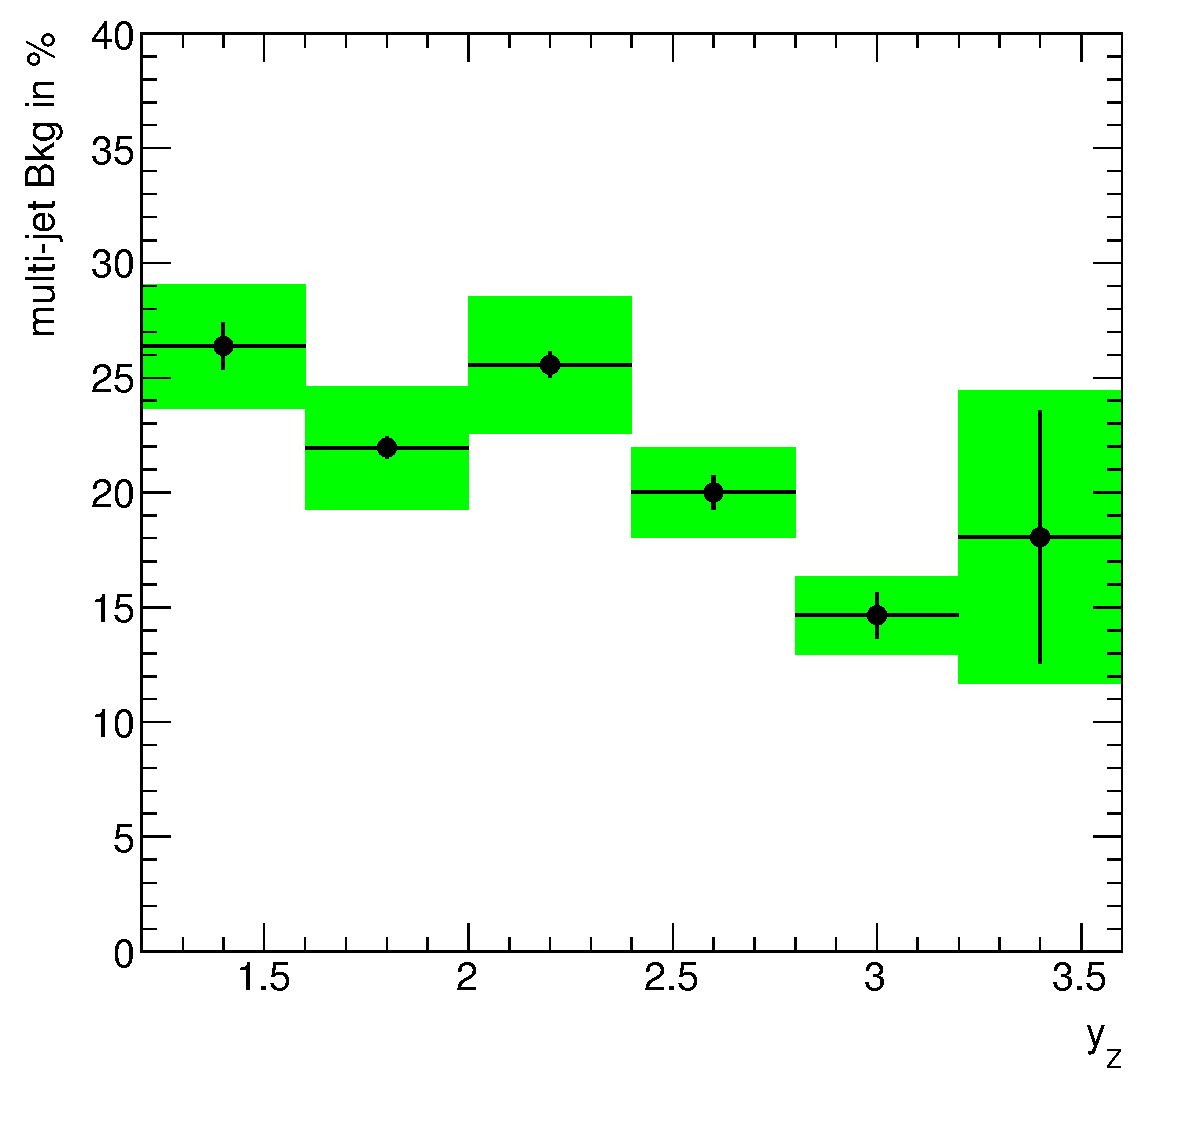
\includegraphics[width=0.45\textwidth]{figures/bkg_qcd_high.pdf}}
\caption{The QCD background estimation for the \Zee\ central-forward analysis, (a) for peak mass and (b) for high mass.}
\label{fig:bkg_qcd}}
\end{figure}

\begin{table}
\centering
\begin{tabular}{ cccc } \hline \hline
 $y_Z$ bin & QCD bkg & Stat & Syst \\  \hline
 1.2 -  1.4 &   2.46 &   0.23  &   0.21 \\
 1.4 -  1.6 &   1.97 &   0.10  &   0.16 \\
 1.6 -  1.8 &   1.93 &   0.09  &   0.16 \\
 1.8 -  2.0 &   1.81 &   0.07  &   0.22 \\
 2.0 -  2.2 &   1.87 &   0.10  &   0.19 \\
 2.2 -  2.4 &   1.86 &   0.08  &   0.07 \\
 2.4 -  2.8 &   1.69 &   0.06  &   0.17 \\
 2.8 -  3.2 &   1.88 &   0.19  &   0.08 \\
 3.2 -  3.6 &   1.43 &   0.26  &   0.25 \\
\hline \hline
\end{tabular}
\caption{The bin-by-bin QCD background astimation for the \Zee\ CF $66 < m_{ee} < 116$~GeV analysis in percents.}
\label{tab:bkg_qcd_peak_percents}
\end{table}

\begin{table}
\centering
\begin{tabular}{ cccc } \hline \hline
 $y_Z$ bin & QCD bkg & Stat & Syst \\  \hline
 1.2 -  1.6 &  26.37 &   1.04  &   2.50 \\
 1.6 -  2.0 &  21.96 &   0.47  &   2.63 \\
 2.0 -  2.4 &  25.57 &   0.57  &   2.95 \\
 2.4 -  2.8 &  20.00 &   0.72  &   1.84 \\
 2.8 -  3.2 &  14.64 &   1.01  &   1.36 \\
 3.2 -  3.6 &  18.07 &   5.53  &   3.17 \\
\hline \hline
\end{tabular}
\caption{The bin-by-bin QCD background astimation for the \Zee\ CF $116 < m_{ee} < 150$~GeV analysis in percents.}
\label{tab:bkg_qcd_high_percents}
\end{table}

The correctness of the background estimation can be seen by the means of the control plots, in which we can compare the amount of the data events that pass all the selection cuts with the luminosity-weighted amount of signal MC together with all sources of the background combined. In Fig.~\ref{fig:Sel_control_Z} the control plot for \Zee\ mass-distribution can be seen. Both peak and high mass regions are presented there. In Figs.~\ref{fig:Sel_control_elecC} and~\ref{fig:Sel_control_elecF} are the control plots for electron $p_T$ distributions for central and forward electrons respectively. In both cases the left plot represents the peak mass region, while the right plot represents the high mass region.

\begin{figure}
\center{
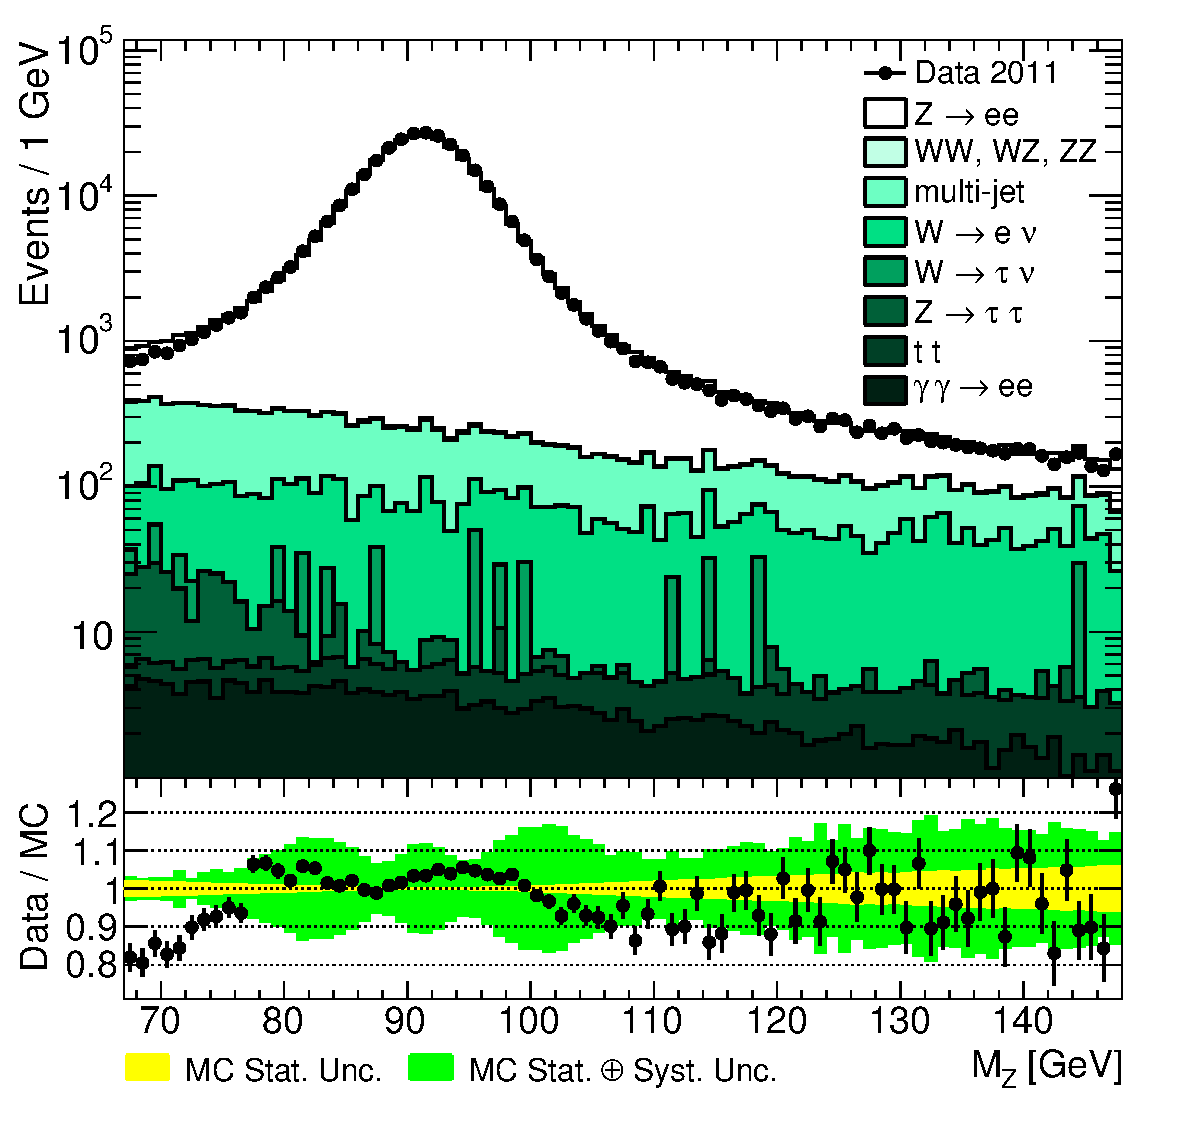
\includegraphics[width=0.6\textwidth]{figures/ZCF_control_BosMass.pdf}
\caption{The comparison between data and MC for \Zee\ mass-distribution for both peak mass and high mass regions.}
\label{fig:Sel_control_Z}}
\end{figure}

\begin{figure}
\center{
  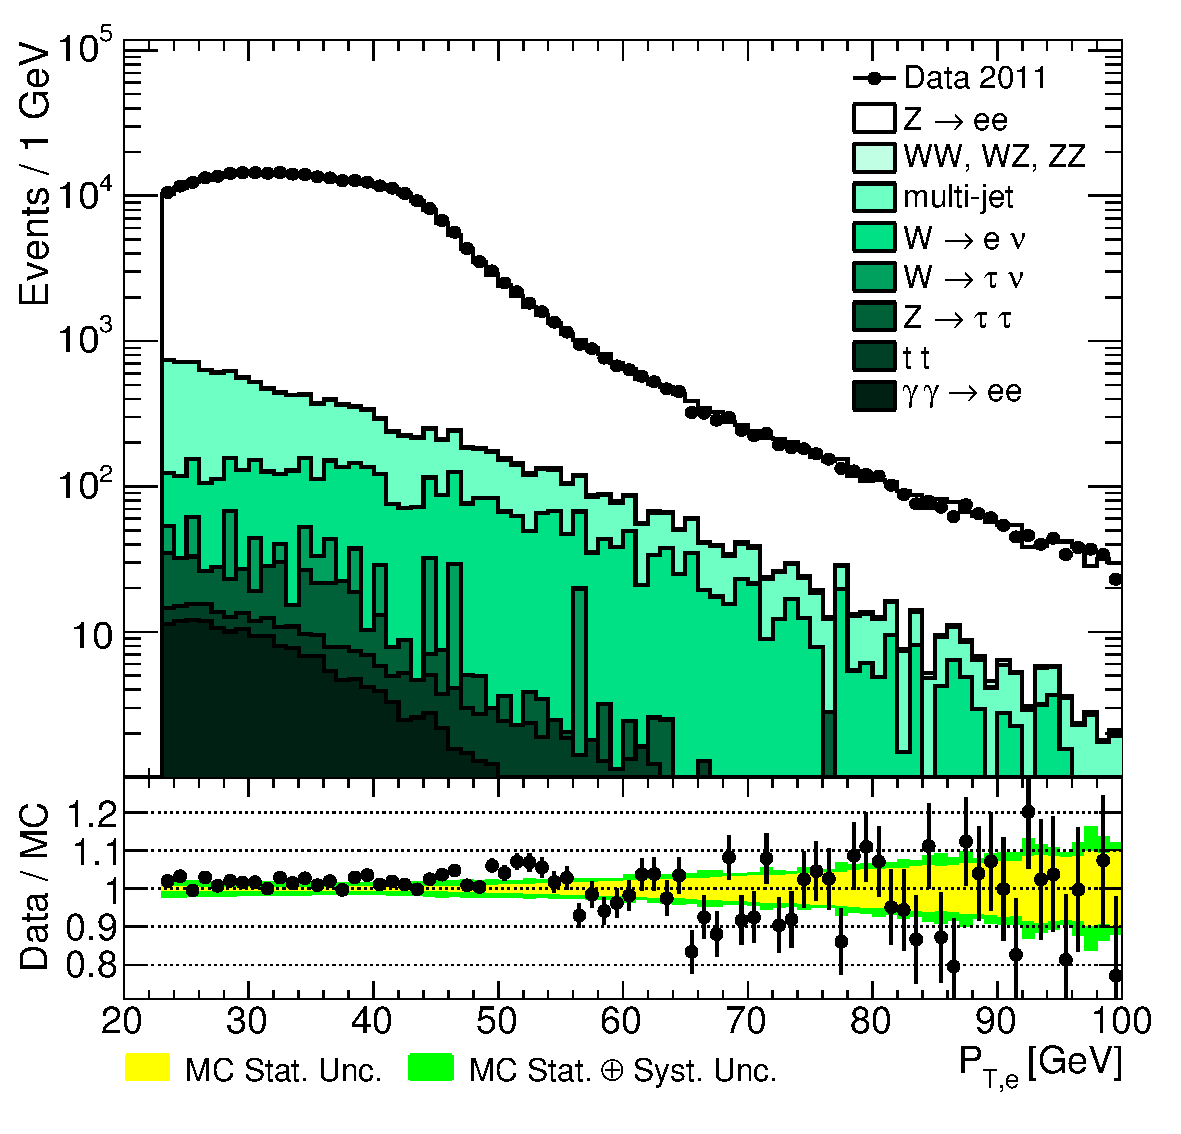
\includegraphics[width=0.45\textwidth]{figures/ZCF_control_ElecPtC_peak.pdf}
  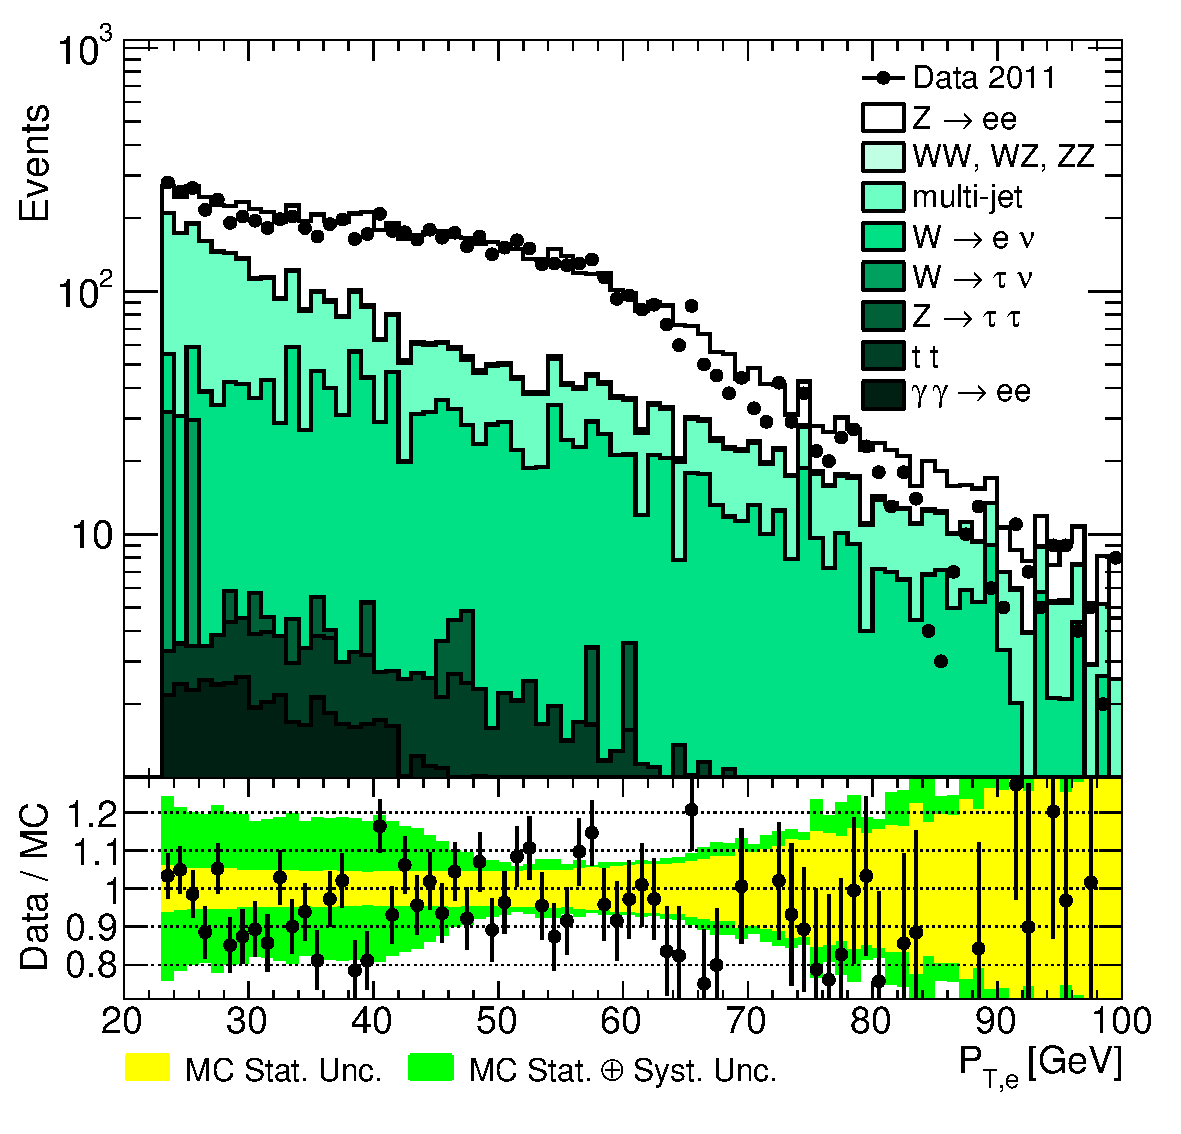
\includegraphics[width=0.45\textwidth]{figures/ZCF_control_ElecPtC_high.pdf}
  \caption{The comparison between data and MC for central electron $p_T$ distribution for peak mass (left) and high mass (right) regions.}
\label{fig:Sel_control_elecC}}
\end{figure}

\begin{figure}
\center{
  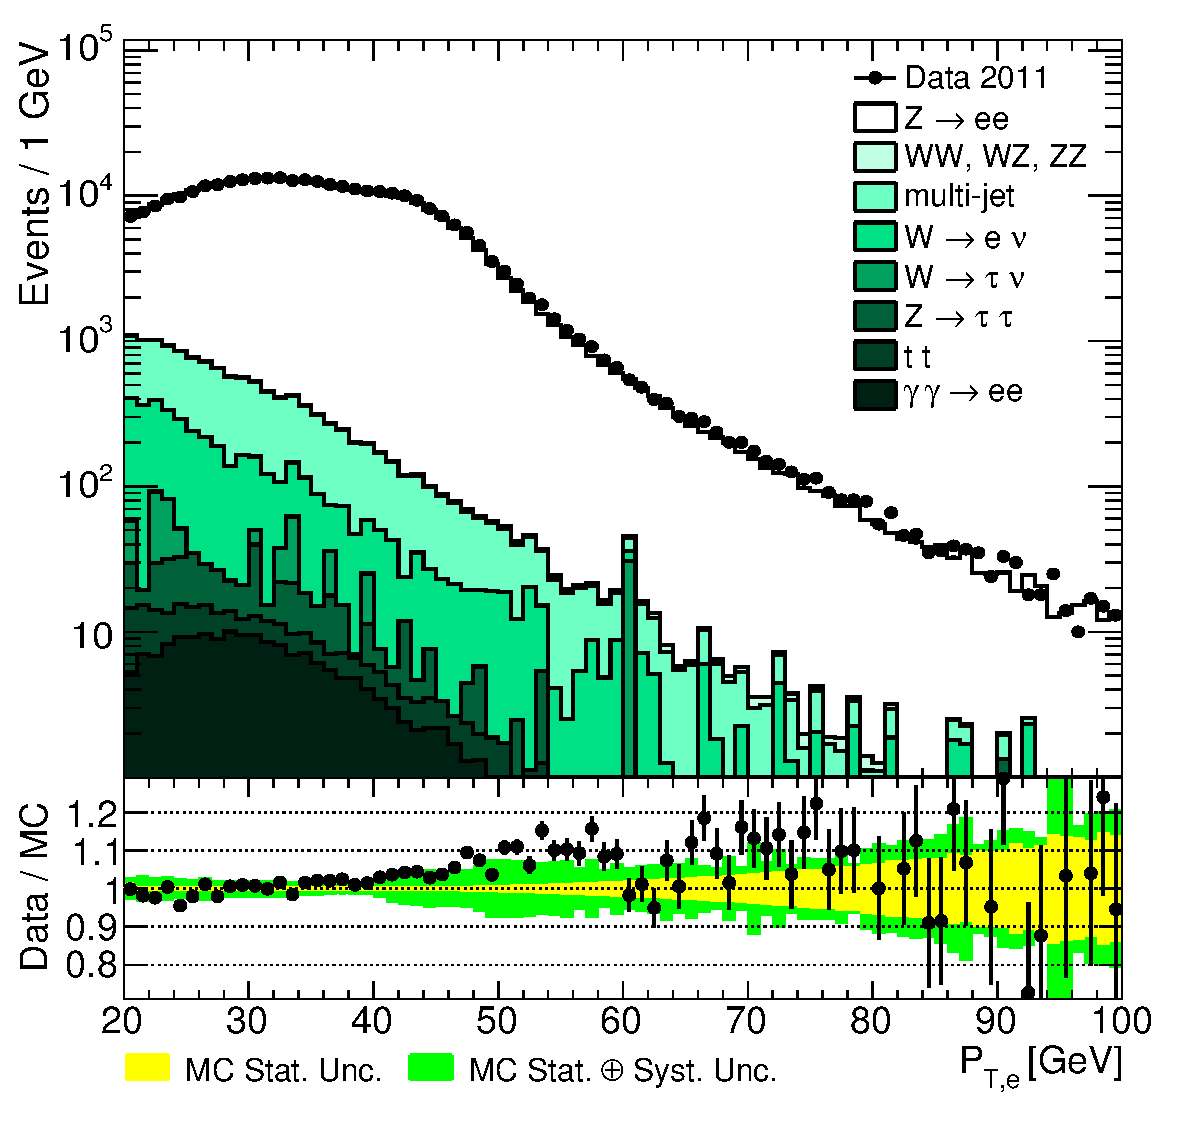
\includegraphics[width=0.45\textwidth]{figures/ZCF_control_ElecPtF_peak.pdf}
  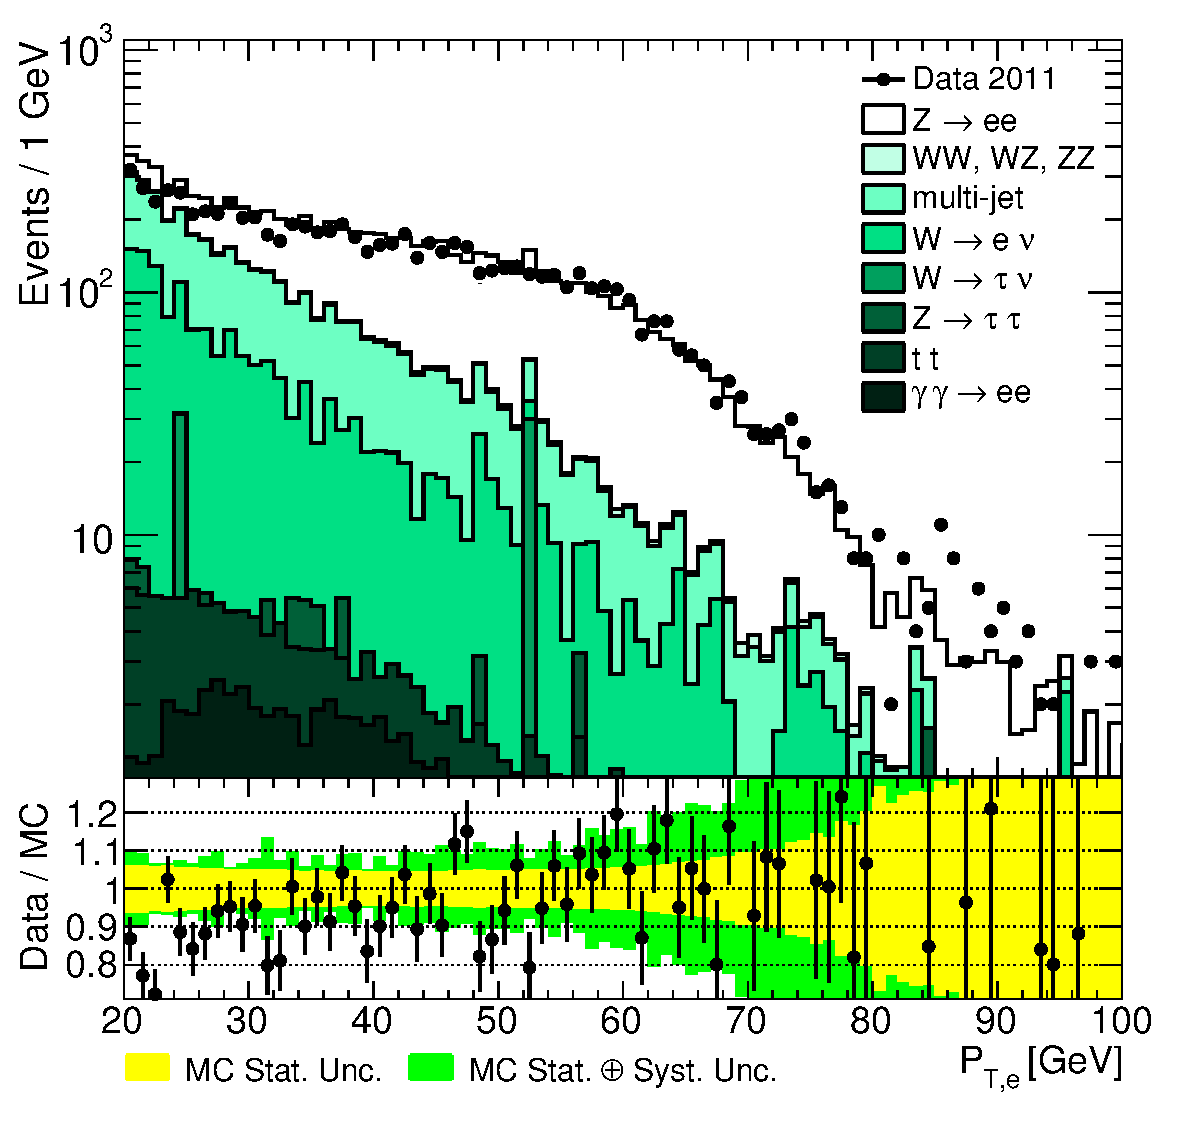
\includegraphics[width=0.45\textwidth]{figures/ZCF_control_ElecPtF_high.pdf}
  \caption{The comparison between data and MC for forward electron $p_T$ distribution for peak mass (left) and high mass (right) regions.}
\label{fig:Sel_control_elecC}}
\end{figure}

\chapter{Results}
\label{sec:Results}

In this section the results of the cross-section calculations are presented. The results of the integral and differential cross-sections (as defined in Sec.~\ref{sec:ZeeCrossSec}) are shown together with uncertainties and theoretical predictions. There are two main types of the uncertainties: statistical and systematical, and whereas the statistical uncertainties are trivial to calculate, and depend only on the amount of the data in any given bin, the sources for the systematical uncertainties are much more numerous. The sources for the different systematical uncertainties are described throughout this thesis, but for the convenience the complete list of them that contributed to the final result is presented in Tab.~\ref{tab:Zee_unc_list_peak} for peak mass region and in Tab.~\ref{tab:Zee_unc_list_high} for high mass region. The systematic uncertainties are also shown at Fig.~\ref{fig:Zee_unc}. Note, that on the image the different uncertainties are just stacked one on top of another, so the total amount of uncertainty shown on the plot in every given bin won't be the same as the resulting uncertainty for that bin, which would require the quadratic sum. From the plots it can be easily seen, that for the peak mass region the uncertainties are largely dominated by the identification efficiency for the forward electron, while in the high mass region the main contributors is the forward electron resolution.

\begin{table}
\centering
\begin{tabular}{l p{0.6cm}p{0.6cm}p{0.6cm}p{0.6cm}p{0.6cm}p{0.6cm}p{0.6cm}p{0.6cm}l}
\hline \hline
   & 1.20, & 1.40, & 1.60, & 1.80, & 2.00, & 2.20, & 2.40, & 2.80, & 3.20, \\
   & 1.40 & 1.60 & 1.80 & 2.00 & 2.20 & 2.40 & 2.80 & 3.20 & 3.60  \\
\hline
Trigger efficiency            & 0.159 & 0.072 & 0.067 & 0.064 & 0.070 & 0.068 & 0.089 & 0.115 & 0.220 \\
Recon. efficiency             & 0.499 & 0.370 & 0.340 & 0.251 & 0.180 & 0.122 & 0.093 & 0.149 & 0.307 \\
Id. efficiency                & 0.258 & 0.223 & 0.210 & 0.166 & 0.157 & 0.133 & 0.164 & 0.216 & 0.436 \\
Id.Fwd efficiency             & 3.215 & 2.898 & 2.641 & 2.450 & 2.070 & 1.840 & 1.634 & 5.443 & 6.991 \\
Iso. efficiency               & 0.090 & 0.082 & 0.078 & 0.091 & 0.064 & 0.077 & 0.067 & 0.067 & 0.179 \\
Electron resolution           & 0.073 & 0.029 & 0.046 & 0.008 & 0.051 & 0.072 & 0.023 & 0.010 & 0.117 \\
Fwd Electron resolution       & 0.984 & 0.696 & 0.513 & 1.727 & 2.632 & 1.883 & 3.002 & 0.451 & 0.353 \\
Electron scale                & 0.438 & 0.277 & 0.186 & 0.212 & 0.255 & 0.154 & 0.114 & 0.097 & 0.247 \\
Fwd Electron scale            & 0.410 & 0.243 & 0.124 & 0.042 & 0.161 & 0.096 & 0.156 & 0.432 & 2.114 \\
Matrix element                & 0.138 & 0.138 & 0.138 & 0.138 & 0.138 & 0.138 & 0.138 & 0.138 & 0.138 \\
PS and hadronization          & 0.522 & 0.522 & 0.522 & 0.522 & 0.522 & 0.521 & 0.521 & 0.521 & 0.521 \\
PDF                           & 0.124 & 0.057 & 0.031 & 0.015 & 0.015 & 0.010 & 0.007 & 0.021 & 0.057 \\
EW Bkg                        & 0.386 & 0.325 & 0.197 & 0.163 & 0.156 & 0.132 & 0.120 & 0.064 & 0.029 \\
QCD Bkg                       & 0.228 & 0.174 & 0.177 & 0.248 & 0.220 & 0.083 & 0.187 & 0.093 & 0.289 \\
\hline
Stat. Uncertainty (MC)        & 0.635 & 0.353 & 0.207 & 0.206 & 0.186 & 0.175 & 0.126 & 0.199 & 0.453 \\
Stat. Uncertainty             & 1.763 & 1.019 & 0.730 & 0.595 & 0.580 & 0.499 & 0.339 & 0.494 & 1.227 \\
\hline
Tot. Syst. Uncertainty        & 3.540 & 3.107 & 2.797 & 3.084 & 3.426 & 2.707 & 3.480 & 5.515 & 7.368 \\
\hline \hline
\end{tabular}
\caption{The list of the uncertainties in percent for peak mass region.}
\label{tab:Zee_unc_list_peak}
\end{table}

\begin{table}
\centering
\begin{tabular}{l r r r r r r}
\hline \hline
   & \multicolumn{1}{l}{1.20,} & \multicolumn{1}{l}{1.60,} & \multicolumn{1}{l}{2.00,}
   & \multicolumn{1}{l}{2.40,} & \multicolumn{1}{l}{2.80,} & \multicolumn{1}{l}{3.20,}  \\
   & 1.60  & 2.00  & 2.40  & 2.80  & 3.20  & 3.60  \\
\hline
Trigger efficiency            & 0.067 & 0.037 & 0.058 & 0.109 & 0.139 & 0.191  \\
Recon. efficiency             & 0.195 & 0.158 & 0.147 & 0.142 & 0.137 & 0.135  \\
Id. efficiency                & 0.132 & 0.113 & 0.170 & 0.246 & 0.256 & 0.243  \\
Id.Fwd efficiency             & 2.463 & 1.919 & 1.517 & 1.955 & 5.330 & 7.069  \\
Iso. efficiency               & 0.046 & 0.053 & 0.080 & 0.096 & 0.078 & 0.079  \\
Electron resolution           & 0.459 & 0.714 & 0.672 & 1.254 & 1.102 & 0.753  \\
Fwd Electron resolution       & 2.357 & 5.231 & 12.303 & 20.601 & 14.154 & 1.554  \\
Electron scale                & 0.302 & 0.354 & 0.717 & 0.592 & 0.609 & 1.607  \\
Fwd Electron scale            & 1.470 & 1.884 & 2.252 & 2.086 & 2.497 & 2.566  \\
Matrix element                & 0.606 & 0.568 & 0.429 & 0.494 & 0.488 & 0.565  \\
PS and hadronization          & 1.480 & 1.385 & 1.048 & 1.208 & 1.195 & 1.397  \\
PDF                           & 0.162 & 0.081 & 0.110 & 0.074 & 0.099 & 0.471  \\
EW Bkg                        & 8.332 & 6.544 & 2.880 & 2.144 & 1.184 & 0.000  \\
QCD Bkg                       & 5.904 & 5.575 & 5.417 & 3.043 & 1.828 & 10.225  \\
\hline
Stat. Uncertainty (MC)        & 1.619 & 1.156 & 0.981 & 0.930 & 1.716 & 3.892  \\
Stat. Uncertainty             & 6.845 & 5.213 & 4.023 & 3.886 & 5.291 & 14.533  \\
\hline
Tot. Syst. Uncertainty        & 11.044 & 10.576 & 14.109 & 21.221 & 15.594 & 13.012 \\
\hline \hline
\end{tabular}
\caption{The list of the uncertainties in percent for high mass region.}
\label{tab:Zee_unc_list_high}
\end{table}

\begin{figure}
\center{
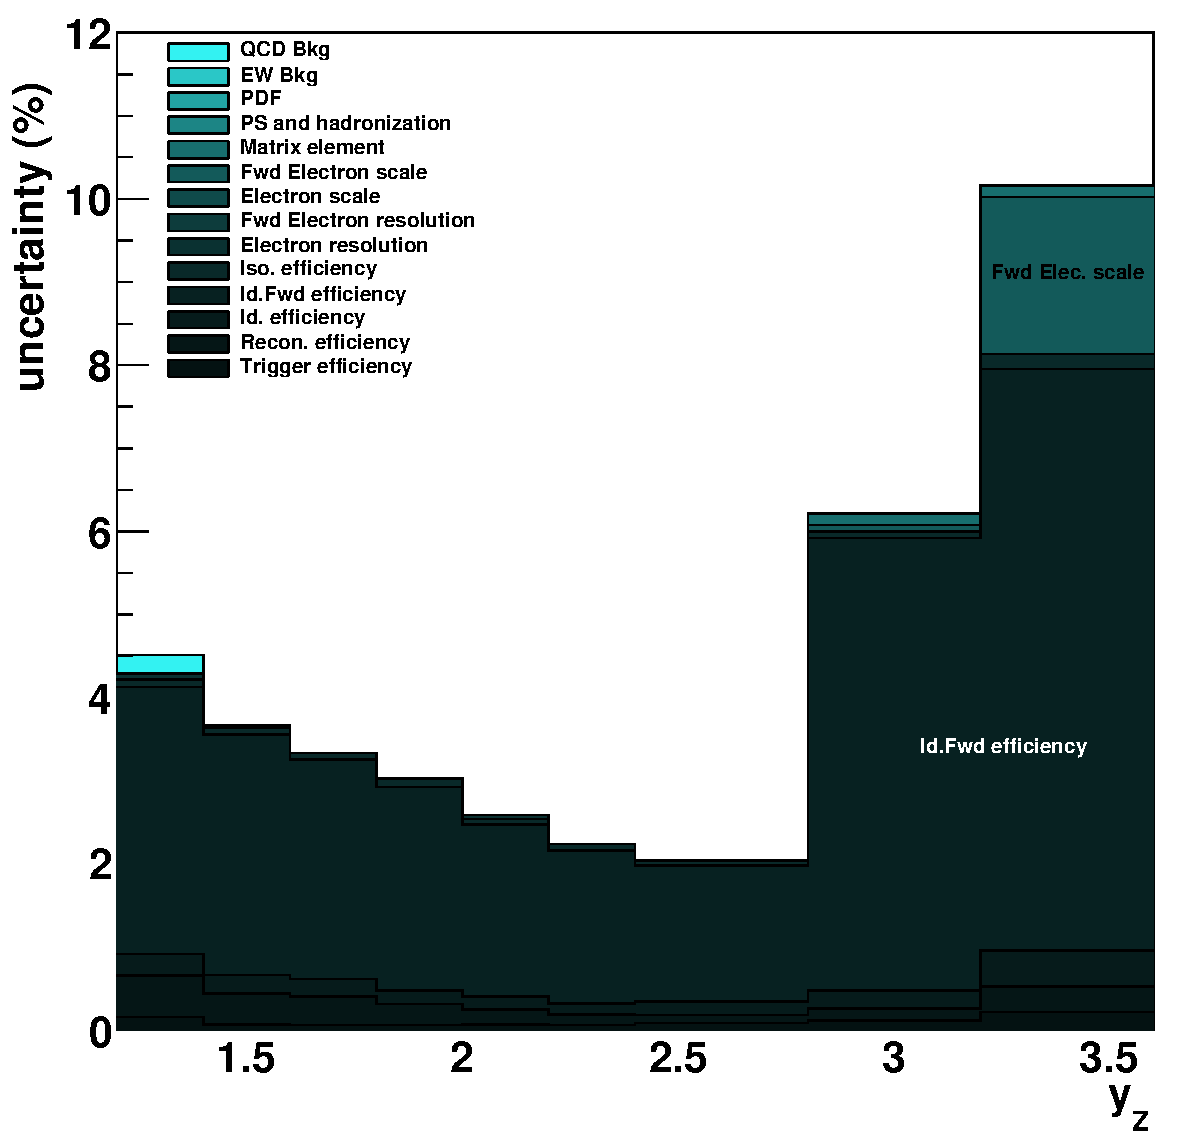
\includegraphics[width=0.45\textwidth]{figures/ZCF_unc_66_116.pdf}
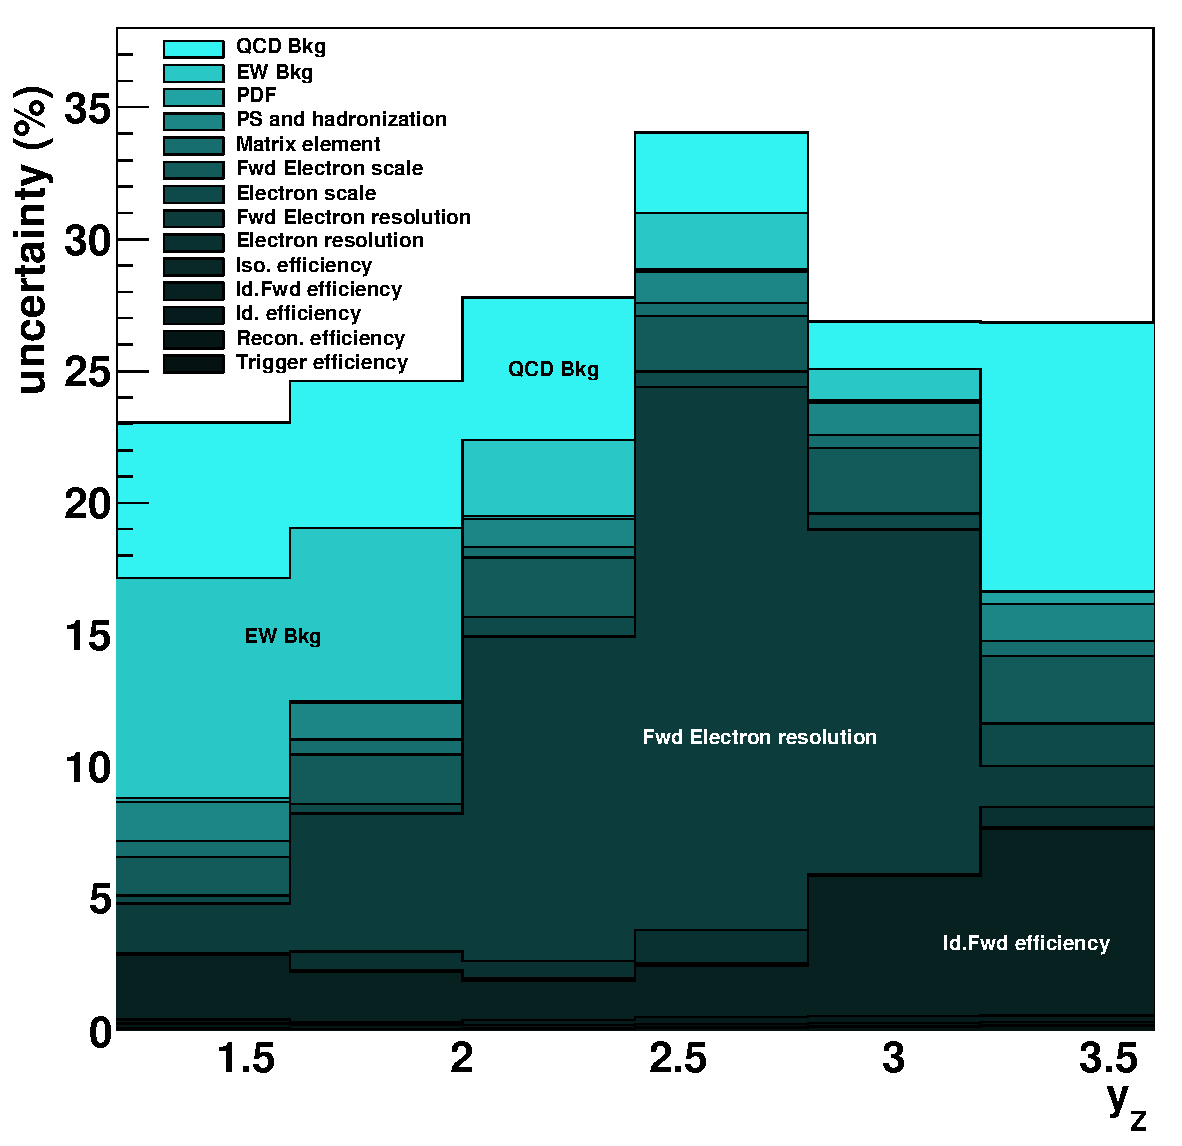
\includegraphics[width=0.45\textwidth]{figures/ZCF_unc_116_150.pdf}
\caption{The list of the systematic uncertainties for the \Zee\ CF analysis for peak mass (left) and high mass (right) regions. The largest sources are explicitly labeled. Each following uncertainty is placed on top of the previous.}
\label{fig:Zee_unc}}
\end{figure}

As the work that was done as part of this thesis contributed to the W,Z inclusive paper~\cite{lib:wz2011} the combined \Zee\ and \Zll\ results were taken from there. The theory comparison that was done for the combined \Zll\ results was outside of the scope of this thesis.

The double-differential analyses were done in the rapidity and mass binning with three mass windows. The \Zee\ central-forward analysis contributed only to two of them: the peak mass ($66 < M_{ee} < 116$~GeV) and the high mass ($116 < M_{ee} < 150$~GeV) windows. Unlike the central-central analysis, the peak mass windows was not divided into additional bins. The analyses results were first calculated in the true experimental fiducial volume, which equals to the experimental phase space and is described in Tab.~\ref{tab:res_phase_space}. Fig.~\ref{fig:res_zee_fid} shows the double-differential cross-section with statistical and systematical uncertainties, and Fig.~\ref{fig:res_zee_fid_mc} shows the comparison with the different MC simulations. The \Powheg\Pythia\ MC simulation was the one used as signal MC, while the others were used as sources for systematical uncertainties.

\begin{table}
\centering
\begin{tabular}{l l}
\hline \hline
Central electron & $p_T > 23$~GeV, \\
\rule{0pt}{4ex}  & $|\eta| < 2.47$ \\
                 & {\bf excluding} \\
                 & $1.37 < |\eta| < 1.52$ \& $1.6 < |\eta| < 1.7$ \\
\hline
Forward electron & $p_T > 20$~GeV, \\
\rule{0pt}{4ex}  & $2.5 < |\eta| < 4.9$ \\
                 & {\bf excluding} \\
                 & $3.16 < |\eta| < 3.35$ \\
\hline
Mass windows     & $66 < m_{ee} < 116$ \& $116 < m_{ee} < 150$ \\
\hline \hline
\end{tabular}
\caption{The conditions of the experimental phase space.}
\label{tab:res_phase_space}
\end{table}


\begin{figure}
\center{
  \includegraphics[width=0.45\textwidth]{figures/ZeeCF_Mass_66_116.pdf}
  \includegraphics[width=0.45\textwidth]{figures/ZeeCF_Mass_116_150.pdf}
  \caption{\Zee\ CF true experimental fiducial differential cross-section, as a function of absolute boson rapidity for peak mass (left) and high mass (right) regions together with statistical and systematic uncertainties.}
\label{fig:res_zee_fid}}
\end{figure}

\begin{figure}
\center{
\includegraphics[width=0.45\textwidth]{figures/ZeeCF_Mass_66_116_MC.pdf}
\includegraphics[width=0.45\textwidth]{figures/ZeeCF_Mass_116_150_MC.pdf}
\caption{\Zee\ CF true experimental fiducial differential cross-section, as a function of absolute boson rapidity for peak mass (left) and high mass (right) regions compared to various MC simulations.}
\label{fig:res_zee_fid_mc}}
\end{figure}

The same results in tabular form can be seen in Tabs.~\ref{tab:Zee_NBC_peak} and~\ref{tab:Zee_NBC_high}, where $N$ is the number of events in the bin, $B$ is the estimated number of the background events included in $N$, and $C$ is the true experimental fiducial extrapolation factor, which represents the fraction of all the $Z$ boson that $N$ amounts to.

\begin{table}
\centering
\begin{tabular}{lccc}
\hline \hline
    &   $N$   & $B \pm \delta B$  &  $C \pm \delta C$ \\
\hline
$1.20 < |y| <1.40$          & 4178       & 193.7      $\pm$ 19.7 & 0.381      $\pm$ 0.014 \\
$1.40 < |y| <1.60$          & 12404      & 517.7      $\pm$ 47.4 & 0.436      $\pm$ 0.013 \\
$1.60 < |y| <1.80$          & 24210      & 812.1      $\pm$ 72.7 & 0.453      $\pm$ 0.012 \\
$1.80 < |y| <2.00$          & 33978      & 1021.2     $\pm$ 110.9 & 0.459      $\pm$ 0.014 \\
$2.00 < |y| <2.20$          & 38023      & 1141.2     $\pm$ 123.9 & 0.449      $\pm$ 0.015 \\
$2.20 < |y| <2.40$          & 51372      & 1454.4     $\pm$ 77.6 & 0.429      $\pm$ 0.011 \\
$2.40 < |y| <2.80$          & 101004     & 2613.2     $\pm$ 267.5 & 0.440      $\pm$ 0.015 \\
$2.80 < |y| <3.20$          & 47304      & 1104.4     $\pm$ 52.3 & 0.384      $\pm$ 0.021 \\
$3.20 < |y| <3.60$          & 8453       & 126.6      $\pm$ 29.5 & 0.276      $\pm$ 0.020 \\
\hline \hline
\end{tabular}
\caption{Main components of the differential \Zee\ CF cross-section for peak mass region.}
\label{tab:Zee_NBC_peak}
\end{table}

\begin{table}
\centering
\begin{tabular}{lccc}
\hline \hline
    &   $N$   & $B \pm \delta B$  &  $C \pm \delta C$ \\
\hline
$1.20 < |y| <1.60$          & 1136       & 592.4      $\pm$ 54.8 & 0.552      $\pm$ 0.024 \\
$1.60 < |y| <2.00$          & 1676       & 754.6      $\pm$ 79.2 & 0.565      $\pm$ 0.035 \\
$2.00 < |y| <2.40$          & 2006       & 737.4      $\pm$ 80.2 & 0.531      $\pm$ 0.067 \\
$2.40 < |y| <2.80$          & 1754       & 506.2      $\pm$ 48.6 & 0.515      $\pm$ 0.107 \\
$2.80 < |y| <3.20$          & 659        & 120.7      $\pm$ 12.8 & 0.439      $\pm$ 0.068 \\
$3.20 < |y| <3.60$          & 84         & 15.2       $\pm$ 8.3 & 0.348      $\pm$ 0.031 \\
\hline \hline
\end{tabular}
\caption{Main components of the differential \Zee\ CF cross-section for high mass region.}
\label{tab:Zee_NBC_high}
\end{table}

In Tabs.~\ref{tab:Zee_peak} and~\ref{tab:Zee_high} the results of the cross-section as measured in the true experimental fiducial volume can be found along with statistical, systematical and luminosity uncertainties.

\begin{table}
\centering
\begin{tabular}{lc}
\hline \hline
$1.20 < |y| <1.40$          & 5.715 $\pm$ 0.101 (stat) $\pm$ 0.207 (syst) $\pm$ 0.103 (lum) [pb]  \\
$1.40 < |y| <1.60$          & 14.864 $\pm$ 0.151 (stat) $\pm$ 0.465 (syst) $\pm$ 0.268 (lum) [pb]  \\
$1.60 < |y| <1.80$          & 28.200 $\pm$ 0.206 (stat) $\pm$ 0.792 (syst) $\pm$ 0.508 (lum) [pb]  \\
$1.80 < |y| <2.00$          & 39.245 $\pm$ 0.233 (stat) $\pm$ 1.214 (syst) $\pm$ 0.706 (lum) [pb]  \\
$2.00 < |y| <2.20$          & 44.786 $\pm$ 0.260 (stat) $\pm$ 1.534 (syst) $\pm$ 0.806 (lum) [pb]  \\
$2.20 < |y| <2.40$          & 63.598 $\pm$ 0.317 (stat) $\pm$ 1.717 (syst) $\pm$ 1.145 (lum) [pb]  \\
$2.40 < |y| <2.80$          & 61.087 $\pm$ 0.207 (stat) $\pm$ 2.126 (syst) $\pm$ 1.100 (lum) [pb]  \\
$2.80 < |y| <3.20$          & 32.826 $\pm$ 0.162 (stat) $\pm$ 1.811 (syst) $\pm$ 0.591 (lum) [pb]  \\
$3.20 < |y| <3.60$          & 8.313 $\pm$ 0.102 (stat) $\pm$ 0.614 (syst) $\pm$ 0.150 (lum) [pb]  \\
\hline \hline
\end{tabular}
\caption{Differential \Zee\ CF cross-section for the peak mass region, measured in the true experimental fiducial volume together with uncertainties.}
\label{tab:Zee_peak}
\end{table}

\begin{table}
\centering
\begin{tabular}{lc}
\hline \hline
$1.20 < |y| <1.60$          & 0.271 $\pm$ 0.018 (stat) $\pm$ 0.030 (syst) $\pm$ 0.005 (lum) [pb]  \\
$1.60 < |y| <2.00$          & 0.454 $\pm$ 0.023 (stat) $\pm$ 0.047 (syst) $\pm$ 0.008 (lum) [pb]  \\
$2.00 < |y| <2.40$          & 0.680 $\pm$ 0.027 (stat) $\pm$ 0.095 (syst) $\pm$ 0.012 (lum) [pb]  \\
$2.40 < |y| <2.80$          & 0.697 $\pm$ 0.027 (stat) $\pm$ 0.147 (syst) $\pm$ 0.013 (lum) [pb]  \\
$2.80 < |y| <3.20$          & 0.367 $\pm$ 0.019 (stat) $\pm$ 0.057 (syst) $\pm$ 0.007 (lum) [pb]  \\
$3.20 < |y| <3.60$          & 0.064 $\pm$ 0.009 (stat) $\pm$ 0.009 (syst) $\pm$ 0.001 (lum) [pb]  \\
\hline \hline
\end{tabular}
\caption{Differential \Zee\ CF cross-section for the high mass region, measured in the true experimental fiducial volume together with uncertainties.}
\label{tab:Zee_high}
\end{table}

For the comparison with the theoretical predictions, the results were extrapolated to the fiducial volume, which differs from the true experimental fiducial volume in inclusion of the crack regions. As a result, the values are about $\sim$20\% higher as in the true experimental one. Fig.~\ref{fig:res_zee_fid_th} shows the comparison to the theoretical predictions done with various PDF sets.

\begin{figure}
\center{
\includegraphics[width=0.45\textwidth]{figures/ZeeCF_Mass_66_116_th.pdf}
\includegraphics[width=0.45\textwidth]{figures/ZeeCF_Mass_116_150_th.pdf}
\caption{\Zee\ CF extrapolated fiducial cross-section, as a function of absolute boson rapidity for peak mass (left) and high mass (right) regions compared to various theoretical predictions.}
\label{fig:res_zee_fid_th}}
\end{figure}

The following results for the \Zll\ combined cross sections were taken from the W,Z inclusive paper~\cite{lib:wz2011}, as the combination of the results was outside of the scope of this thesis. The combination technique was described in Sec.~\ref{sec:ZeeCS_comb}. It is important to note, that \Zee\ central-forward data contributed only to the $|y| > 1.2$ part of the combined cross-section, and the last three bins $|y| > 2.4$ of it can be seen as purely \Zee\ central-forward. The combined cross-section itself can be seen in Fig.~\ref{fig:Zll}, while the comparison with the different theoretical predictions can be seen in Fig.~\ref{fig:Zll_theory}.

\begin{figure}
\center{
  \includegraphics[width=0.45\textwidth]{figures/Z_66_116_combined.pdf}
  \includegraphics[width=0.45\textwidth]{figures/Z_116_150_combined.pdf}
  \caption{Combined \Zll\ cross-section for peak mass (left) and high mass (right) regions together with uncertainties. The ratio and the pull values are also shown for each source.~\cite{lib:wz2011}}
\label{fig:Zll}}
\end{figure}

\begin{figure}
\center{
  \includegraphics[width=0.45\textwidth]{figures/Z_66_116_NNLO_combined.pdf}
  \includegraphics[width=0.45\textwidth]{figures/Z_116_150_NNLO_combined.pdf}
  \caption{Comparison of the combined \Zll\ cross-section with NNLO predictions using various PDF sets for peak mass (left) and high mass (right) regions together with uncertainties. The ratios are also shown.~\cite{lib:wz2011}}
\label{fig:Zll_theory}}
\end{figure}

\chapter{Summary}
\label{sec:Summary}

This thesis represented the results of the \Zee\ central-forward cross-section measurement based on the $4.6 \mathrm{fb}^{-1}$ of the data collected on the ATLAS detector of the LHC during the 2011 year.

In order to get these results some technical solutions were developed for both ATLAS software infrastructure and the analysis software itself. For the ATLAS software the Frozen Showers system was developed. This system reduced the amount of time needed for the Monte Carlo simulation by about 25\% while introducing a small error that was well within the uncertainties introduced by the technical limitations of the detector. The Frozen Shower system was enabled by default in all the Monte Carlo samples starting with the 2011 for all the analyses. The MC samples used in this analysis were also produced with Frozen Showers enabled.

For the analysis software the new TTree system was developed that was used for data storage. This system reduced the amount of space needed for data samples from terabytes to gigabytes and subsequently allowed to launch the analysis software on local machines and reduced the time needed for the analysis. With the TTree input the ZeeD software was able to process 1000 events per second which makes a couple of hours for the whole dataset, instead of several days that the same task would take while on the GRID reading from the raw AODs. The analysis presented in this thesis was done using the TTree system.

The different stages of the analysis included the identification of the electrons, finding of the boson candidates, filtering of the \Zee\ events based on several criteria (cuts), estimating of the background and the unfolding. Each stage was described in a separate chapter, presenting its impact on the result and the possible sources of the uncertainties it adds. The resulting double-differential \Zee\ central-forward cross-section  together with all sources of uncertainties was presented. This cross-section agrees well with the results of \Zee\ central-central and \Zmm\ analyses, and in combination with them can be used for a future improvement of PDF sets.


\newpage
\phantomsection
\begin{tiny}
  \listoffigures
\end{tiny}


\newpage
\phantomsection
\bibliographystyle{atlasBibStyleWithTitle}
\bibliography{Thesis}

\newpage
\chapter*{Acknowledgements}

If you bothered to read this far, you'll probably be here, don't worry :)
\newline\newline\newline
\raisebox{-0.3\height}{\includegraphics[height=\baselineskip]{figures/like.png}} Like if you opened the thesis only to read this page.

\end{document}
